% Options for packages loaded elsewhere
\PassOptionsToPackage{unicode}{hyperref}
\PassOptionsToPackage{hyphens}{url}
\PassOptionsToPackage{dvipsnames,svgnames,x11names}{xcolor}
\documentclass[
  10pt,
]{article}
\usepackage{xcolor}
\usepackage[left=2cm, right=2cm, top=2cm, bottom=3cm, footskip = .5cm]{geometry}
\usepackage{amsmath,amssymb}
\setcounter{secnumdepth}{-\maxdimen} % remove section numbering
\usepackage{iftex}
\ifPDFTeX
  \usepackage[T1]{fontenc}
  \usepackage[utf8]{inputenc}
  \usepackage{textcomp} % provide euro and other symbols
\else % if luatex or xetex
  \usepackage{unicode-math} % this also loads fontspec
  \defaultfontfeatures{Scale=MatchLowercase}
  \defaultfontfeatures[\rmfamily]{Ligatures=TeX,Scale=1}
\fi
\usepackage{lmodern}
\ifPDFTeX\else
  % xetex/luatex font selection
\fi
% Use upquote if available, for straight quotes in verbatim environments
\IfFileExists{upquote.sty}{\usepackage{upquote}}{}
\IfFileExists{microtype.sty}{% use microtype if available
  \usepackage[]{microtype}
  \UseMicrotypeSet[protrusion]{basicmath} % disable protrusion for tt fonts
}{}
\makeatletter
\@ifundefined{KOMAClassName}{% if non-KOMA class
  \IfFileExists{parskip.sty}{%
    \usepackage{parskip}
  }{% else
    \setlength{\parindent}{0pt}
    \setlength{\parskip}{6pt plus 2pt minus 1pt}}
}{% if KOMA class
  \KOMAoptions{parskip=half}}
\makeatother
\usepackage{longtable,booktabs,array}
\usepackage{calc} % for calculating minipage widths
% Correct order of tables after \paragraph or \subparagraph
\usepackage{etoolbox}
\makeatletter
\patchcmd\longtable{\par}{\if@noskipsec\mbox{}\fi\par}{}{}
\makeatother
% Allow footnotes in longtable head/foot
\IfFileExists{footnotehyper.sty}{\usepackage{footnotehyper}}{\usepackage{footnote}}
\makesavenoteenv{longtable}
\usepackage{graphicx}
\makeatletter
\newsavebox\pandoc@box
\newcommand*\pandocbounded[1]{% scales image to fit in text height/width
  \sbox\pandoc@box{#1}%
  \Gscale@div\@tempa{\textheight}{\dimexpr\ht\pandoc@box+\dp\pandoc@box\relax}%
  \Gscale@div\@tempb{\linewidth}{\wd\pandoc@box}%
  \ifdim\@tempb\p@<\@tempa\p@\let\@tempa\@tempb\fi% select the smaller of both
  \ifdim\@tempa\p@<\p@\scalebox{\@tempa}{\usebox\pandoc@box}%
  \else\usebox{\pandoc@box}%
  \fi%
}
% Set default figure placement to htbp
\def\fps@figure{htbp}
\makeatother
\setlength{\emergencystretch}{3em} % prevent overfull lines
\providecommand{\tightlist}{%
  \setlength{\itemsep}{0pt}\setlength{\parskip}{0pt}}
% Set up the fonts
\usepackage[urw-palatino]{mathdesign}
\usepackage[T1]{fontenc}

% Add accessibility support from http://www.richschwinn.com/accessibility
\RequirePackage{accsupp}
\RequirePackage{pdfcomment}
\newcommand{\AccTool}[2]{\BeginAccSupp{method=pdfstringdef,unicode,Alt={{#1}}}\pdftooltip{{#2}}{{#1}}\EndAccSupp{}}

% Set the language for 508
\hypersetup{
  pdftitle = {title},
  pdflang = en-US}
 
% left-align all figure captions 
\usepackage{caption}
\captionsetup{justification=raggedright,singlelinecheck=false}
  
% Set up the headers and footers
\usepackage{graphicx}
\usepackage{fancyhdr}
\usepackage{ifthen}
%\usepackage{everypage-1x}
\usepackage{float}
%\usepackage{subfig}
%\usepackage{subcaption}

% Avoid struggling over figure and table float in Rmarkdown
\let\origfigure\figure
\let\endorigfigure\endfigure
\renewenvironment{figure}[1][2] {
    \expandafter\origfigure\expandafter[H]
} {
    \endorigfigure
}

\let\origtable\table
\let\endorigtable\endtable
\renewenvironment{table}[1][2] {
    \expandafter\origtable\expandafter[H]
} {
    \endorigtable
}

% First page has the large title and NOAA logo
\pagestyle{fancy}
\fancyhf{}
\setlength\headheight{40pt}
\fancyheadoffset[L]{0.5cm}
\cfoot{\thepage}

\fancyheadinit{%
   \ifthenelse{\value{page}=4}%
      {\fancyhead[R]{
\includegraphics[width=40pt]{images/NOAA_logo.png} \\ \textsf{\emph{March 18, 2026}}}
       \fancyhead[L]{\textsf{\LARGE State of the Ecosystem 2026: Mid-Atlantic}}
      }%
      {\fancyhead[R]{}
       \fancyhead[L]{\textsf{\emph{State of the Ecosystem 2026: Mid-Atlantic}}}
      }
}



\renewcommand{\headrulewidth}{0.4pt}
\renewcommand{\footrulewidth}{0pt}

% Make caption fonts a bit smaller
\usepackage[font={small}]{caption}


% Change section labels to san serif
\usepackage{sectsty}
\allsectionsfont{\normalfont\sffamily\bfseries}
\usepackage{float}
\usepackage{multirow}
\usepackage{multicol}
\usepackage{colortbl}
\usepackage{ulem}
\usepackage{hhline}
\newlength\Oldarrayrulewidth
\newlength\Oldtabcolsep
\usepackage{longtable}
\usepackage{array}
\usepackage{hyperref}
\usepackage{wrapfig}
\usepackage{bookmark}
\IfFileExists{xurl.sty}{\usepackage{xurl}}{} % add URL line breaks if available
\urlstyle{same}
\hypersetup{
  colorlinks=true,
  linkcolor={Maroon},
  filecolor={Maroon},
  citecolor={Blue},
  urlcolor={blue},
  pdfcreator={LaTeX via pandoc}}

\author{}
\date{\vspace{-2.5em}}

\begin{document}

\setcounter{page}{6}
\thispagestyle{fancy}

\section{Introduction}\label{introduction}

\subsection{About This Report}\label{about-this-report}

This report is for the Mid-Atlantic Fishery Management Council (MAFMC). The purpose of this report is to synthesize ecosystem information to allow the MAFMC to better meet fishery management objectives, and to update the MAFMC's Ecosystem Approach to Fishery Management (EAFM) risk assessment. The major messages of the report are synthesized on pages 1 and 2, with highlights of 2025 ecosystem events on page 3.

The information in this report is organized into two main sections; \hyperref[performance-relative-to-fishery-management-objectives]{performance measured against ecosystem-level management objectives} (Table \ref{tab:management-objectives}), and potential \hyperref[risks-to-meeting-fishery-management-objectives]{risks to meeting fishery management objectives} (Table \ref{tab:management-risks}: \hyperref[climate-and-ecosystem-change]{climate change} and \hyperref[other-ocean-uses-offshore-wind]{other ocean uses}). A final section highlights \hyperref[highlights]{notable 2025 ecosystem observations}.

\subsection{Report structure}\label{report-structure}

A glossary of terms\footnote{\url{https://noaa-edab.github.io/tech-doc/glossary.html}}, detailed technical methods documentation\footnote{\url{https://noaa-edab.github.io/tech-doc/}}, indicator data\footnote{\url{https://noaa-edab.github.io/ecodata/}}, and detailed indicator descriptions\footnote{\url{https://noaa-edab.github.io/catalog/index.html}} are available online. We recommend new readers first review the details of standard figure formatting (Fig. \ref{fig:docformat}a), categorization of fish and invertebrate species into feeding guilds (Table \ref{tab:species-groupings}), and definitions of ecological production units (EPUs, including the Mid-Atlantic Bight, MAB; Fig. \ref{fig:docformat}b) provided at the end of the document.

The two main sections contain subsections for each management objective or potential risk. Within each subsection, we first review observed trends for indicators representing each objective or risk, including the status of the most recent data year relative to a threshold (if available) or relative to the long-term average. Second, we identify potential drivers of observed trends, and synthesize results of indicators related to those drivers to outline potential implications for management. For example, if there are multiple drivers related to an indicator trend, do indicators associated with the drivers have similar trends, and can any drivers be affected by management action(s)? We emphasize that these implications are intended to represent testable hypotheses at present, rather than ``answers,'' because the science behind these indicators and syntheses continues to develop.

All indicators are updated with the most recent data available as of January 2026, and all indicators are updated with the same data years across both reports. In some cases, indicators are only updated through 2024 due to data availability. In these cases, we still include the indicator in the report to provide context for the most recent data year and to allow for future updates.

Because this report is intended to provide a high-level overview of marine ecosystem information in the Northeast United States, we do not include complete methods or detailed results for all of the indicators that we present. More information can be found hyperlinked in blue text.

\newpage

\global\setlength{\Oldarrayrulewidth}{\arrayrulewidth}

\global\setlength{\Oldtabcolsep}{\tabcolsep}

\setlength{\tabcolsep}{2pt}

\renewcommand*{\arraystretch}{1.5}



\providecommand{\ascline}[3]{\noalign{\global\arrayrulewidth #1}\arrayrulecolor[HTML]{#2}\cline{#3}}

\begin{longtable}[c]{|p{1.77in}|p{4.47in}}

\caption{Ecosystem-scale\ fishery\ management\ objectives\ in\ the\ Mid-Atlantic\ Bight}\label{tab:management-objectives}\\

\ascline{1.5pt}{666666}{1-2}

\multicolumn{1}{>{\raggedright}m{\dimexpr 1.77in+0\tabcolsep}}{\textcolor[HTML]{000000}{\fontsize{9}{9}\selectfont{Objective\ categories}}} & \multicolumn{1}{>{\raggedright}m{\dimexpr 4.47in+0\tabcolsep}}{\textcolor[HTML]{000000}{\fontsize{9}{9}\selectfont{Indicators\ reported}}} \\

\ascline{1.5pt}{666666}{1-2}\endfirsthead \caption[]{Ecosystem-scale\ fishery\ management\ objectives\ in\ the\ Mid-Atlantic\ Bight}\label{tab:management-objectives}\\

\ascline{1.5pt}{666666}{1-2}

\multicolumn{1}{>{\raggedright}m{\dimexpr 1.77in+0\tabcolsep}}{\textcolor[HTML]{000000}{\fontsize{9}{9}\selectfont{Objective\ categories}}} & \multicolumn{1}{>{\raggedright}m{\dimexpr 4.47in+0\tabcolsep}}{\textcolor[HTML]{000000}{\fontsize{9}{9}\selectfont{Indicators\ reported}}} \\

\ascline{1.5pt}{666666}{1-2}\endhead



\multicolumn{2}{>{\raggedright}m{\dimexpr 6.24in+2\tabcolsep}}{\textcolor[HTML]{000000}{\fontsize{9}{9}\selectfont{\textbf{Objectives:\ Provisioning\ and\ Cultural\ Services}}}} \\





\multicolumn{1}{>{\raggedright}m{\dimexpr 1.77in+0\tabcolsep}}{\textcolor[HTML]{000000}{\fontsize{9}{9}\selectfont{Seafood\ Production}}} & \multicolumn{1}{>{\raggedright}m{\dimexpr 4.47in+0\tabcolsep}}{\textcolor[HTML]{000000}{\fontsize{9}{9}\selectfont{Landings;\ commercial\ total\ and\ by\ feeding\ guild;\ recreational\ harvest}}} \\





\multicolumn{1}{>{\raggedright}m{\dimexpr 1.77in+0\tabcolsep}}{\textcolor[HTML]{000000}{\fontsize{9}{9}\selectfont{Commercial\ Profits}}} & \multicolumn{1}{>{\raggedright}m{\dimexpr 4.47in+0\tabcolsep}}{\textcolor[HTML]{000000}{\fontsize{9}{9}\selectfont{Revenue\ decomposed\ to\ price\ and\ volume}}} \\





\multicolumn{1}{>{\raggedright}m{\dimexpr 1.77in+0\tabcolsep}}{\textcolor[HTML]{000000}{\fontsize{9}{9}\selectfont{Recreational\ Opportunities}}} & \multicolumn{1}{>{\raggedright}m{\dimexpr 4.47in+0\tabcolsep}}{\textcolor[HTML]{000000}{\fontsize{9}{9}\selectfont{Angler\ trips;\ recreational\ fleet\ diversity}}} \\





\multicolumn{1}{>{\raggedright}m{\dimexpr 1.77in+0\tabcolsep}}{\textcolor[HTML]{000000}{\fontsize{9}{9}\selectfont{Stability}}} & \multicolumn{1}{>{\raggedright}m{\dimexpr 4.47in+0\tabcolsep}}{\textcolor[HTML]{000000}{\fontsize{9}{9}\selectfont{Fishery\ and\ ecosystem\ volatility,\ adaptive\ capacity,\ and\ shifts\ from\ baseline}}} \\





\multicolumn{1}{>{\raggedright}m{\dimexpr 1.77in+0\tabcolsep}}{\textcolor[HTML]{000000}{\fontsize{9}{9}\selectfont{Social\ \&\ Cultural}}} & \multicolumn{1}{>{\raggedright}m{\dimexpr 4.47in+0\tabcolsep}}{\textcolor[HTML]{000000}{\fontsize{9}{9}\selectfont{Community\ commercial\ fishing\ activity\ and\ risk\ factors}}} \\





\multicolumn{1}{>{\raggedright}m{\dimexpr 1.77in+0\tabcolsep}}{\textcolor[HTML]{000000}{\fontsize{9}{9}\selectfont{Protected\ Species}}} & \multicolumn{1}{>{\raggedright}m{\dimexpr 4.47in+0\tabcolsep}}{\textcolor[HTML]{000000}{\fontsize{9}{9}\selectfont{Bycatch;\ population\ (adult\ and\ juvenile)\ numbers;\ mortalities}}} \\





\multicolumn{2}{>{\raggedright}m{\dimexpr 6.24in+2\tabcolsep}}{\textcolor[HTML]{000000}{\fontsize{9}{9}\selectfont{\textbf{Potential\ Drivers:\ Supporting\ and\ Regulating\ Services}}}} \\





\multicolumn{1}{>{\raggedright}m{\dimexpr 1.77in+0\tabcolsep}}{\textcolor[HTML]{000000}{\fontsize{9}{9}\selectfont{Management}}} & \multicolumn{1}{>{\raggedright}m{\dimexpr 4.47in+0\tabcolsep}}{\textcolor[HTML]{000000}{\fontsize{9}{9}\selectfont{Stock\ status;\ catch\ compared\ with\ catch\ limits}}} \\





\multicolumn{1}{>{\raggedright}m{\dimexpr 1.77in+0\tabcolsep}}{\textcolor[HTML]{000000}{\fontsize{9}{9}\selectfont{Biomass}}} & \multicolumn{1}{>{\raggedright}m{\dimexpr 4.47in+0\tabcolsep}}{\textcolor[HTML]{000000}{\fontsize{9}{9}\selectfont{Biomass\ or\ abundance\ by\ feeding\ guild\ from\ surveys}}} \\





\multicolumn{1}{>{\raggedright}m{\dimexpr 1.77in+0\tabcolsep}}{\textcolor[HTML]{000000}{\fontsize{9}{9}\selectfont{Environment}}} & \multicolumn{1}{>{\raggedright}m{\dimexpr 4.47in+0\tabcolsep}}{\textcolor[HTML]{000000}{\fontsize{9}{9}\selectfont{Climate\ and\ ecosystem\ risk\ indicators\ listed\ in\ Table\ 2}}} \\

\ascline{1.5pt}{666666}{1-2}



\end{longtable}



\arrayrulecolor[HTML]{000000}

\global\setlength{\arrayrulewidth}{\Oldarrayrulewidth}

\global\setlength{\tabcolsep}{\Oldtabcolsep}

\renewcommand*{\arraystretch}{1}

\global\setlength{\Oldarrayrulewidth}{\arrayrulewidth}

\global\setlength{\Oldtabcolsep}{\tabcolsep}

\setlength{\tabcolsep}{2pt}

\renewcommand*{\arraystretch}{1.5}



\providecommand{\ascline}[3]{\noalign{\global\arrayrulewidth #1}\arrayrulecolor[HTML]{#2}\cline{#3}}

\begin{longtable}[c]{|p{1.00in}|p{2.19in}|p{2.81in}}

\caption{Risks\ to\ meeting\ fishery\ management\ objectives\ in\ the\ Mid-Atlantic\ Bight}\label{tab:management-risks}\\

\ascline{1.5pt}{666666}{1-3}

\multicolumn{1}{>{\raggedright}m{\dimexpr 1in+0\tabcolsep}}{\textcolor[HTML]{000000}{\fontsize{9}{9}\selectfont{Risk\ categories}}} & \multicolumn{1}{>{\raggedright}m{\dimexpr 2.19in+0\tabcolsep}}{\textcolor[HTML]{000000}{\fontsize{9}{9}\selectfont{Observation\ indicators\ reported}}} & \multicolumn{1}{>{\raggedright}m{\dimexpr 2.81in+0\tabcolsep}}{\textcolor[HTML]{000000}{\fontsize{9}{9}\selectfont{Potential\ driver\ indicators\ reported}}} \\

\ascline{1.5pt}{666666}{1-3}\endfirsthead \caption[]{Risks\ to\ meeting\ fishery\ management\ objectives\ in\ the\ Mid-Atlantic\ Bight}\label{tab:management-risks}\\

\ascline{1.5pt}{666666}{1-3}

\multicolumn{1}{>{\raggedright}m{\dimexpr 1in+0\tabcolsep}}{\textcolor[HTML]{000000}{\fontsize{9}{9}\selectfont{Risk\ categories}}} & \multicolumn{1}{>{\raggedright}m{\dimexpr 2.19in+0\tabcolsep}}{\textcolor[HTML]{000000}{\fontsize{9}{9}\selectfont{Observation\ indicators\ reported}}} & \multicolumn{1}{>{\raggedright}m{\dimexpr 2.81in+0\tabcolsep}}{\textcolor[HTML]{000000}{\fontsize{9}{9}\selectfont{Potential\ driver\ indicators\ reported}}} \\

\ascline{1.5pt}{666666}{1-3}\endhead



\multicolumn{3}{>{\raggedright}m{\dimexpr 6in+4\tabcolsep}}{\textcolor[HTML]{000000}{\fontsize{9}{9}\selectfont{\textbf{Climate\ and\ Ecosystem\ Risks}}}} \\





\multicolumn{1}{>{\raggedright}m{\dimexpr 1in+0\tabcolsep}}{\textcolor[HTML]{000000}{\fontsize{9}{9}\selectfont{Risks\ to\ Managing\ Spatially}}} & \multicolumn{1}{>{\raggedright}m{\dimexpr 2.19in+0\tabcolsep}}{\textcolor[HTML]{000000}{\fontsize{9}{9}\selectfont{Managed\ species\ (fish\ and\ cetacean)\ distribution\ shifts}}} & \multicolumn{1}{>{\raggedright}m{\dimexpr 2.81in+0\tabcolsep}}{\textcolor[HTML]{000000}{\fontsize{9}{9}\selectfont{Benthic\ and\ pelagic\ forage\ distribution;\ ocean\ temperature,\ changes\ in\ currents\ and\ Cold\ Pool}}} \\





\multicolumn{1}{>{\raggedright}m{\dimexpr 1in+0\tabcolsep}}{\textcolor[HTML]{000000}{\fontsize{9}{9}\selectfont{Risks\ to\ Managing\ Seasonally}}} & \multicolumn{1}{>{\raggedright}m{\dimexpr 2.19in+0\tabcolsep}}{\textcolor[HTML]{000000}{\fontsize{9}{9}\selectfont{Managed\ species\ spawning\ and\ migration\ timing\ changes}}} & \multicolumn{1}{>{\raggedright}m{\dimexpr 2.81in+0\tabcolsep}}{\textcolor[HTML]{000000}{\fontsize{9}{9}\selectfont{Habitat\ timing:\ Length\ of\ ocean\ summer,\ Cold\ Pool\ seasonal\ persistence}}} \\





\multicolumn{1}{>{\raggedright}m{\dimexpr 1in+0\tabcolsep}}{\textcolor[HTML]{000000}{\fontsize{9}{9}\selectfont{Risks\ to\ Setting\ Catch\ Limits}}} & \multicolumn{1}{>{\raggedright}m{\dimexpr 2.19in+0\tabcolsep}}{\textcolor[HTML]{000000}{\fontsize{9}{9}\selectfont{Managed\ species\ body\ condition\ and\ recruitment\ changes}}} & \multicolumn{1}{>{\raggedright}m{\dimexpr 2.81in+0\tabcolsep}}{\textcolor[HTML]{000000}{\fontsize{9}{9}\selectfont{Benthic\ and\ pelagic\ forage\ quality\ \&\ abundance;\ ocean\ temperature\ \&\ acidification\ }}} \\





\multicolumn{3}{>{\raggedright}m{\dimexpr 6in+4\tabcolsep}}{\textcolor[HTML]{000000}{\fontsize{9}{9}\selectfont{\textbf{Other\ Ocean\ Uses\ Risks}}}} \\





\multicolumn{1}{>{\raggedright}m{\dimexpr 1in+0\tabcolsep}}{\textcolor[HTML]{000000}{\fontsize{9}{9}\selectfont{Offshore\ Wind\ Risks}}} & \multicolumn{1}{>{\raggedright}m{\dimexpr 2.19in+0\tabcolsep}}{\textcolor[HTML]{000000}{\fontsize{9}{9}\selectfont{Fishery\ revenue\ and\ landings\ from\ wind\ lease\ areas\ by\ species\ and\ port}}} & \multicolumn{1}{>{\raggedright}m{\dimexpr 2.81in+0\tabcolsep}}{\textcolor[HTML]{000000}{\fontsize{9}{9}\selectfont{Wind\ development\ map;\ Protected\ species\ presence\ and\ hotspots}}} \\

\ascline{1.5pt}{666666}{1-3}



\end{longtable}



\arrayrulecolor[HTML]{000000}

\global\setlength{\arrayrulewidth}{\Oldarrayrulewidth}

\global\setlength{\tabcolsep}{\Oldtabcolsep}

\renewcommand*{\arraystretch}{1}

\subsection{Document Orientation}\label{document-orientation}

The figure format is illustrated in Fig \ref{fig:docformat}a. Both long-term and short-term trends are assessed and plotted if \href{https://noaa-edab.github.io/tech-doc/trend-analysis.html}{statistically significant} at the p \textless{} 0.05 level. An orange line signifies a positive trend, and purple signifies a negative trend. To minimize bias introduced by small sample size, time series with less than 30 years are assessed using the short-term trend methodology applied over the extent of the time period. Dashed lines represent mean values of time series unless the indicator is an anomaly, in which case the dashed line is equal to 0. Shaded regions indicate the past ten years. If there are no new data for the most recent year, the shaded region will still cover this time period. Indicators are scaled at several levels: coastwide; by state groups (Mid-Atlantic: NY, NJ, DE, MD, VA, NC; New England: ME, NH, MA, RI, CT); or by Ecosystem Production Unit (EPU), including the Mid-Atlantic Bight (MAB), Georges Bank (GB), and Gulf of Maine (GOM) (Fig. \ref{fig:docformat}b).

\begin{figure}[T]

{\centering 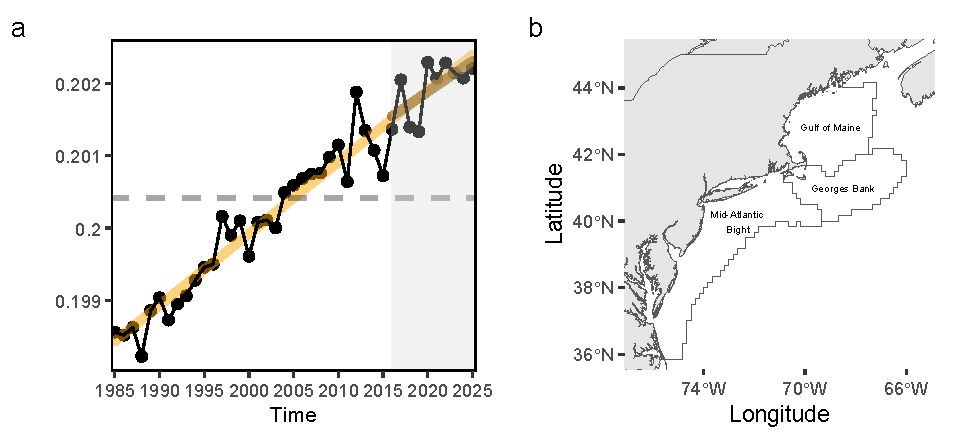
\includegraphics[width=1\linewidth,]{SOE2026_MAFMC_edits_files/figure-latex/docformat-1} 

}

\caption{Document orientation. a) Key to figures: orange line - significant long-term increasing trend (purple for decreasing), dark orange line - significant increasing short-term trend (dark purple for decreasing), dashed line - time-series mean. b)The Northeast Large Marine Ecosystem: Ecological production units (EPUs) defined for the Gulf of Maine (GOM), Georges Bank (GB), and the Mid-Atlantic Bight (MAB).}\label{fig:docformat}
\end{figure}

Fish and invertebrates are aggregated into similar feeding categories (Table \ref{tab:species-groupings}) to evaluate ecosystem level trends in predators and prey.

\global\setlength{\Oldarrayrulewidth}{\arrayrulewidth}

\global\setlength{\Oldtabcolsep}{\tabcolsep}

\setlength{\tabcolsep}{2pt}

\renewcommand*{\arraystretch}{1.5}



\providecommand{\ascline}[3]{\noalign{\global\arrayrulewidth #1}\arrayrulecolor[HTML]{#2}\cline{#3}}

\begin{longtable}[c]{|p{1.00in}|p{1.00in}|p{1.00in}|p{1.00in}|p{3.00in}}

\caption{Feeding\ guilds\ and\ management\ bodies.}\label{tab:species-groupings}\\

\ascline{1.5pt}{666666}{1-5}

\multicolumn{1}{>{\raggedright}m{\dimexpr 1in+0\tabcolsep}}{\textcolor[HTML]{000000}{\fontsize{8}{8}\selectfont{Guild}}} & \multicolumn{1}{>{\raggedright}m{\dimexpr 1in+0\tabcolsep}}{\textcolor[HTML]{000000}{\fontsize{8}{8}\selectfont{MAFMC}}} & \multicolumn{1}{>{\raggedright}m{\dimexpr 1in+0\tabcolsep}}{\textcolor[HTML]{000000}{\fontsize{8}{8}\selectfont{Joint}}} & \multicolumn{1}{>{\raggedright}m{\dimexpr 1in+0\tabcolsep}}{\textcolor[HTML]{000000}{\fontsize{8}{8}\selectfont{NEFMC}}} & \multicolumn{1}{>{\raggedright}m{\dimexpr 3in+0\tabcolsep}}{\textcolor[HTML]{000000}{\fontsize{8}{8}\selectfont{State\ or\ Other}}} \\

\ascline{1.5pt}{666666}{1-5}\endfirsthead \caption[]{Feeding\ guilds\ and\ management\ bodies.}\label{tab:species-groupings}\\

\ascline{1.5pt}{666666}{1-5}

\multicolumn{1}{>{\raggedright}m{\dimexpr 1in+0\tabcolsep}}{\textcolor[HTML]{000000}{\fontsize{8}{8}\selectfont{Guild}}} & \multicolumn{1}{>{\raggedright}m{\dimexpr 1in+0\tabcolsep}}{\textcolor[HTML]{000000}{\fontsize{8}{8}\selectfont{MAFMC}}} & \multicolumn{1}{>{\raggedright}m{\dimexpr 1in+0\tabcolsep}}{\textcolor[HTML]{000000}{\fontsize{8}{8}\selectfont{Joint}}} & \multicolumn{1}{>{\raggedright}m{\dimexpr 1in+0\tabcolsep}}{\textcolor[HTML]{000000}{\fontsize{8}{8}\selectfont{NEFMC}}} & \multicolumn{1}{>{\raggedright}m{\dimexpr 3in+0\tabcolsep}}{\textcolor[HTML]{000000}{\fontsize{8}{8}\selectfont{State\ or\ Other}}} \\

\ascline{1.5pt}{666666}{1-5}\endhead



\multicolumn{1}{>{\raggedright}m{\dimexpr 1in+0\tabcolsep}}{\textcolor[HTML]{000000}{\fontsize{8}{8}\selectfont{Apex\ Predator}}} & \multicolumn{1}{>{\raggedright}m{\dimexpr 1in+0\tabcolsep}}{\textcolor[HTML]{000000}{\fontsize{8}{8}\selectfont{}}} & \multicolumn{1}{>{\raggedright}m{\dimexpr 1in+0\tabcolsep}}{\textcolor[HTML]{000000}{\fontsize{8}{8}\selectfont{}}} & \multicolumn{1}{>{\raggedright}m{\dimexpr 1in+0\tabcolsep}}{\textcolor[HTML]{000000}{\fontsize{8}{8}\selectfont{}}} & \multicolumn{1}{>{\raggedright}m{\dimexpr 3in+0\tabcolsep}}{\textcolor[HTML]{000000}{\fontsize{8}{8}\selectfont{shark\ uncl,\ swordfish,\ yellowfin\ tuna,\ bluefin\ tuna}}} \\





\multicolumn{1}{>{\raggedright}m{\dimexpr 1in+0\tabcolsep}}{\textcolor[HTML]{000000}{\fontsize{8}{8}\selectfont{Piscivore}}} & \multicolumn{1}{>{\raggedright}m{\dimexpr 1in+0\tabcolsep}}{\textcolor[HTML]{000000}{\fontsize{8}{8}\selectfont{summer\ flounder,\ bluefish,\ northern\ shortfin\ squid,\ longfin\ squid}}} & \multicolumn{1}{>{\raggedright}m{\dimexpr 1in+0\tabcolsep}}{\textcolor[HTML]{000000}{\fontsize{8}{8}\selectfont{spiny\ dogfish,\ goosefish}}} & \multicolumn{1}{>{\raggedright}m{\dimexpr 1in+0\tabcolsep}}{\textcolor[HTML]{000000}{\fontsize{8}{8}\selectfont{winter\ skate,\ clearnose\ skate,\ thorny\ skate,\ offshore\ hake,\ silver\ hake,\ atlantic\ cod,\ pollock,\ white\ hake,\ red\ hake,\ atlantic\ halibut,\ windowpane,\ acadian\ redfish}}} & \multicolumn{1}{>{\raggedright}m{\dimexpr 3in+0\tabcolsep}}{\textcolor[HTML]{000000}{\fontsize{8}{8}\selectfont{sea\ lamprey,\ sandbar\ shark,\ atlantic\ angel\ shark,\ atlantic\ torpedo,\ conger\ eel,\ spotted\ hake,\ cusk,\ fourspot\ flounder,\ john\ dory,\ atlantic\ cutlassfish,\ blue\ runner,\ striped\ bass,\ weakfish,\ sea\ raven,\ northern\ stargazer,\ banded\ rudderfish,\ atlantic\ sharpnose\ shark,\ inshore\ lizardfish,\ atlantic\ brief\ squid,\ northern\ sennet,\ king\ mackerel,\ spanish\ mackerel}}} \\





\multicolumn{1}{>{\raggedright}m{\dimexpr 1in+0\tabcolsep}}{\textcolor[HTML]{000000}{\fontsize{8}{8}\selectfont{Planktivore}}} & \multicolumn{1}{>{\raggedright}m{\dimexpr 1in+0\tabcolsep}}{\textcolor[HTML]{000000}{\fontsize{8}{8}\selectfont{atlantic\ mackerel,\ chub\ mackerel,\ butterfish}}} & \multicolumn{1}{>{\raggedright}m{\dimexpr 1in+0\tabcolsep}}{\textcolor[HTML]{000000}{\fontsize{8}{8}\selectfont{}}} & \multicolumn{1}{>{\raggedright}m{\dimexpr 1in+0\tabcolsep}}{\textcolor[HTML]{000000}{\fontsize{8}{8}\selectfont{atlantic\ herring}}} & \multicolumn{1}{>{\raggedright}m{\dimexpr 3in+0\tabcolsep}}{\textcolor[HTML]{000000}{\fontsize{8}{8}\selectfont{harvestfishes,\ smelts,\ round\ herring,\ alewife,\ blueback\ herring,\ american\ shad,\ menhaden,\ bay\ anchovy,\ striped\ anchovy,\ rainbow\ smelt,\ atlantic\ argentine,\ slender\ snipe\ eel,\ atlantic\ silverside,\ northern\ pipefish,\ atlantic\ moonfish,\ lookdown,\ blackbelly\ rosefish,\ lumpfish,\ northern\ sand\ lance,\ atlantic\ saury,\ mackerel\ scad,\ bigeye\ scad,\ round\ scad,\ rough\ scad,\ silver\ rag,\ weitzmans\ pearlsides,\ atlantic\ soft\ pout,\ sevenspine\ bay\ shrimp,\ pink\ glass\ shrimp,\ polar\ lebbeid,\ friendly\ blade\ shrimp,\ bristled\ longbeak,\ aesop\ shrimp,\ norwegian\ shrimp,\ northern\ shrimp,\ brown\ rock\ shrimp,\ atlantic\ thread\ herring,\ spanish\ sardine,\ atlantic\ bumper,\ harvestfish,\ striated\ argentine,\ silver\ anchovy}}} \\





\multicolumn{1}{>{\raggedright}m{\dimexpr 1in+0\tabcolsep}}{\textcolor[HTML]{000000}{\fontsize{8}{8}\selectfont{Benthivore}}} & \multicolumn{1}{>{\raggedright}m{\dimexpr 1in+0\tabcolsep}}{\textcolor[HTML]{000000}{\fontsize{8}{8}\selectfont{black\ sea\ bass,\ scup,\ tilefish}}} & \multicolumn{1}{>{\raggedright}m{\dimexpr 1in+0\tabcolsep}}{\textcolor[HTML]{000000}{\fontsize{8}{8}\selectfont{}}} & \multicolumn{1}{>{\raggedright}m{\dimexpr 1in+0\tabcolsep}}{\textcolor[HTML]{000000}{\fontsize{8}{8}\selectfont{barndoor\ skate,\ rosette\ skate,\ little\ skate,\ smooth\ skate,\ haddock,\ american\ plaice,\ yellowtail\ flounder,\ winter\ flounder,\ witch\ flounder,\ atlantic\ wolffish,\ ocean\ pout,\ crab,red\ deepsea}}} & \multicolumn{1}{>{\raggedright}m{\dimexpr 3in+0\tabcolsep}}{\textcolor[HTML]{000000}{\fontsize{8}{8}\selectfont{crab,unc,\ hagfish,\ porgy,red,\ sea\ bass,nk,\ atlantic\ hagfish,\ roughtail\ stingray,\ smooth\ dogfish,\ chain\ dogfish,\ bluntnose\ stingray,\ bullnose\ ray,\ southern\ stingray,\ longfin\ hake,\ fourbeard\ rockling,\ marlin-spike,\ gulf\ stream\ flounder,\ longspine\ snipefish,\ blackmouth\ bass,\ threespine\ stickleback,\ smallmouth\ flounder,\ hogchoker,\ bigeye,\ atlantic\ croaker,\ pigfish,\ northern\ kingfish,\ silver\ perch,\ spot,\ deepbody\ boarfish,\ sculpin\ uncl,\ moustache\ sculpin,\ longhorn\ sculpin,\ alligatorfish,\ grubby,\ atlantic\ seasnail,\ northern\ searobin,\ striped\ searobin,\ armored\ searobin,\ cunner,\ tautog,\ snakeblenny,\ daubed\ shanny,\ radiated\ shanny,\ red\ goatfish,\ striped\ cusk-eel,\ wolf\ eelpout,\ wrymouth,\ fawn\ cusk-eel,\ northern\ puffer,\ striped\ burrfish,\ planehead\ filefish,\ gray\ triggerfish,\ shortnose\ greeneye,\ beardfish,\ cownose\ ray,\ american\ lobster,\ cancer\ crab\ uncl,\ jonah\ crab,\ atlantic\ rock\ crab,\ blue\ crab,\ spider\ crab\ uncl,\ horseshoe\ crab,\ coarsehand\ lady\ crab,\ lady\ crab,\ northern\ stone\ crab,\ snow\ crab,\ spiny\ butterfly\ ray,\ smooth\ butterfly\ ray,\ snakefish,\ atlantic\ midshipman,\ bank\ cusk-eel,\ red\ cornetfish,\ squid\ cuttlefish\ and\ octopod\ uncl,\ spoonarm\ octopus,\ bank\ sea\ bass,\ rock\ sea\ bass,\ sand\ perch,\ cobia,\ crevalle\ jack,\ vermilion\ snapper,\ tomtate,\ jolthead\ porgy,\ saucereye\ porgy,\ whitebone\ porgy,\ knobbed\ porgy,\ sheepshead\ porgy,\ littlehead\ porgy,\ silver\ porgy,\ pinfish,\ red\ porgy,\ porgy\ and\ pinfish\ uncl,\ banded\ drum,\ southern\ kingfish,\ atlantic\ spadefish,\ leopard\ searobin,\ dusky\ flounder,\ triggerfish\ filefish\ uncl,\ blackcheek\ tonguefish,\ orange\ filefish,\ queen\ triggerfish,\ ocean\ triggerfish}}} \\





\multicolumn{1}{>{\raggedright}m{\dimexpr 1in+0\tabcolsep}}{\textcolor[HTML]{000000}{\fontsize{8}{8}\selectfont{Benthos}}} & \multicolumn{1}{>{\raggedright}m{\dimexpr 1in+0\tabcolsep}}{\textcolor[HTML]{000000}{\fontsize{8}{8}\selectfont{atlantic\ surfclam,\ ocean\ quahog}}} & \multicolumn{1}{>{\raggedright}m{\dimexpr 1in+0\tabcolsep}}{\textcolor[HTML]{000000}{\fontsize{8}{8}\selectfont{}}} & \multicolumn{1}{>{\raggedright}m{\dimexpr 1in+0\tabcolsep}}{\textcolor[HTML]{000000}{\fontsize{8}{8}\selectfont{sea\ scallop}}} & \multicolumn{1}{>{\raggedright}m{\dimexpr 3in+0\tabcolsep}}{\textcolor[HTML]{000000}{\fontsize{8}{8}\selectfont{sea\ cucumber,\ sea\ urchins,\ snails(conchs),\ sea\ urchin\ and\ sand\ dollar\ uncl,\ channeled\ whelk,\ blue\ mussel}}} \\

\ascline{1.5pt}{666666}{1-5}



\end{longtable}



\arrayrulecolor[HTML]{000000}

\global\setlength{\arrayrulewidth}{\Oldarrayrulewidth}

\global\setlength{\tabcolsep}{\Oldtabcolsep}

\renewcommand*{\arraystretch}{1}

\newpage

\section{Performance Relative to Fishery Management Objectives}\label{performance-relative-to-fishery-management-objectives}

In this section, we examine indicators related to broad, ecosystem-level fishery management objectives. We also provide hypotheses on the implications of these trends---why we are seeing them, what's driving them, and potential or observed regime shifts or changes in ecosystem structure. Identifying multiple drivers, regime shifts, and potential changes to ecosystem structure, as well as identifying the most vulnerable resources, can help managers determine whether anything needs to be done differently to meet objectives and how to prioritize upcoming issues/risks.

\subsection{Seafood Production}\label{seafood-production}

\subsubsection{Indicators: Landings; commercial and recreational}\label{indicators-landings-commercial-and-recreational}

In the Mid-Atlantic, total \href{https://noaa-edab.github.io/catalog/comdat.html}{commercial landings} (includes bait and industrial landings) have declined over the long-term, and both total U.S. seafood (excludes bait and industrial uses) and MAFMC-managed seafood landings are at their all time low in 2024 (Fig. \ref{fig:total-landings}). Commercial landings by \href{https://noaa-edab.github.io/catalog/species_groupings.html}{guild} include all species and all uses caught within the MAB, and are reported in total and for MAFMC managed species only. Landings of benthos have been below the long-term average since 2010, primarily driven by surf clam, ocean quahog, and recently scallops. Planktivores show a long-term decline, primarily due to decreases in species not managed by the MAFMC (Atlantic herring and Atlantic menhaden; Fig. \ref{fig:comm-landings}).

\begin{figure}[T]

{\centering 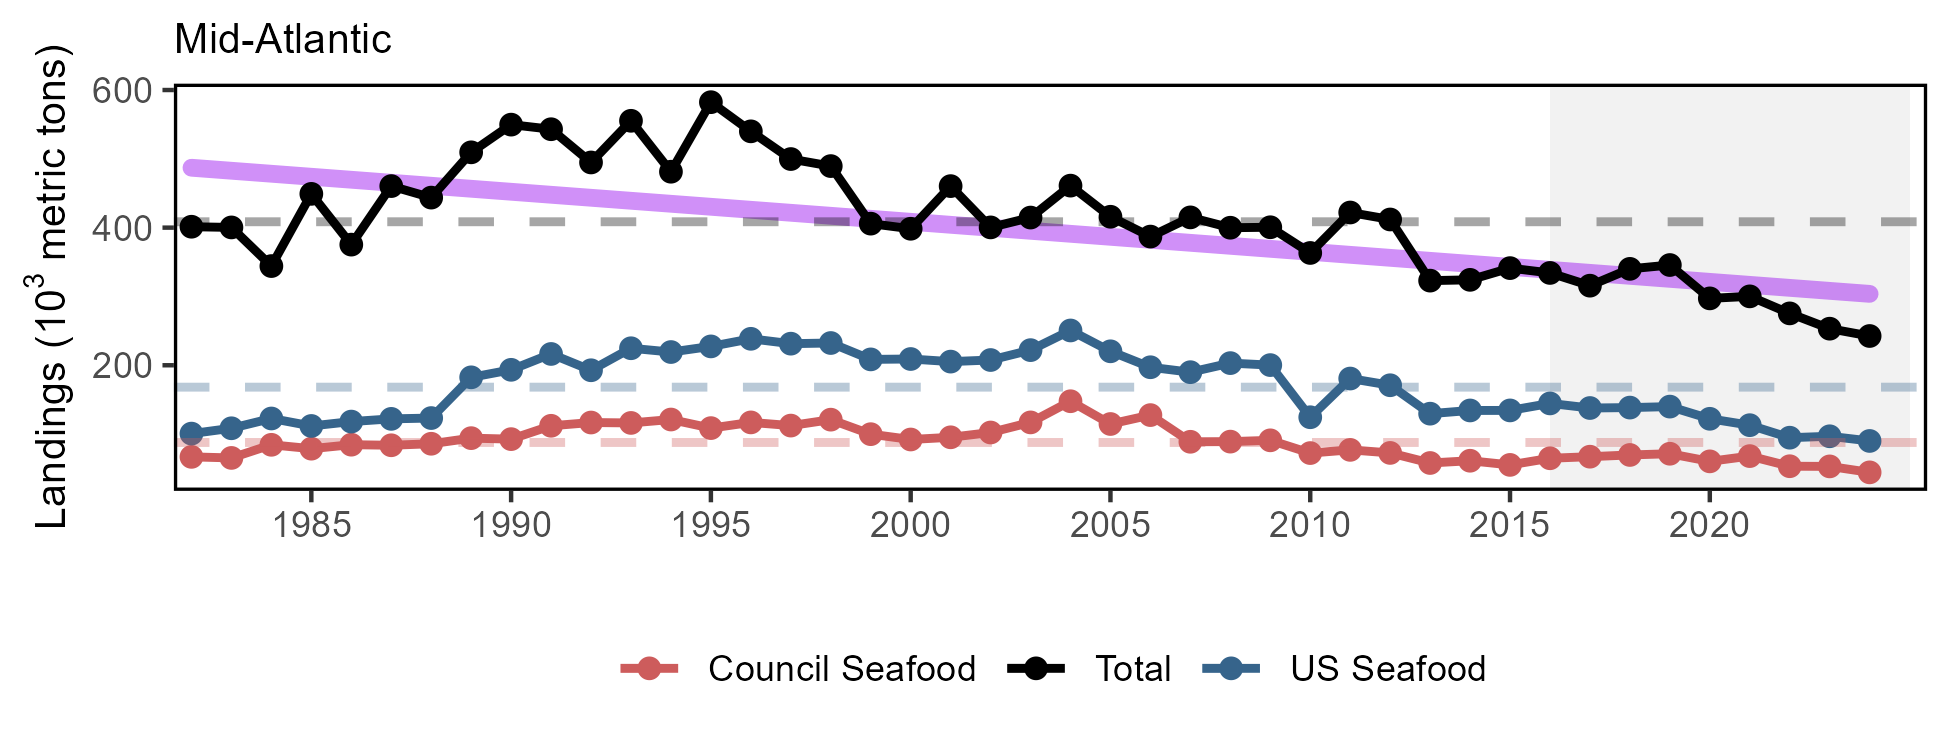
\includegraphics[width=1\linewidth,alt={This is sample alt text},]{images/MidAtlantic/total_landings_MidAtlantic_2026-03-26} 

}

\caption{Total commercial landings (black), total U.S. seafood landings (blue), and Mid-Atlantic managed U.S. seafood landings (red), with long-term significant decline (purple) in total landings.}\label{fig:total-landings}
\end{figure}

\begin{figure}[T]

{\centering 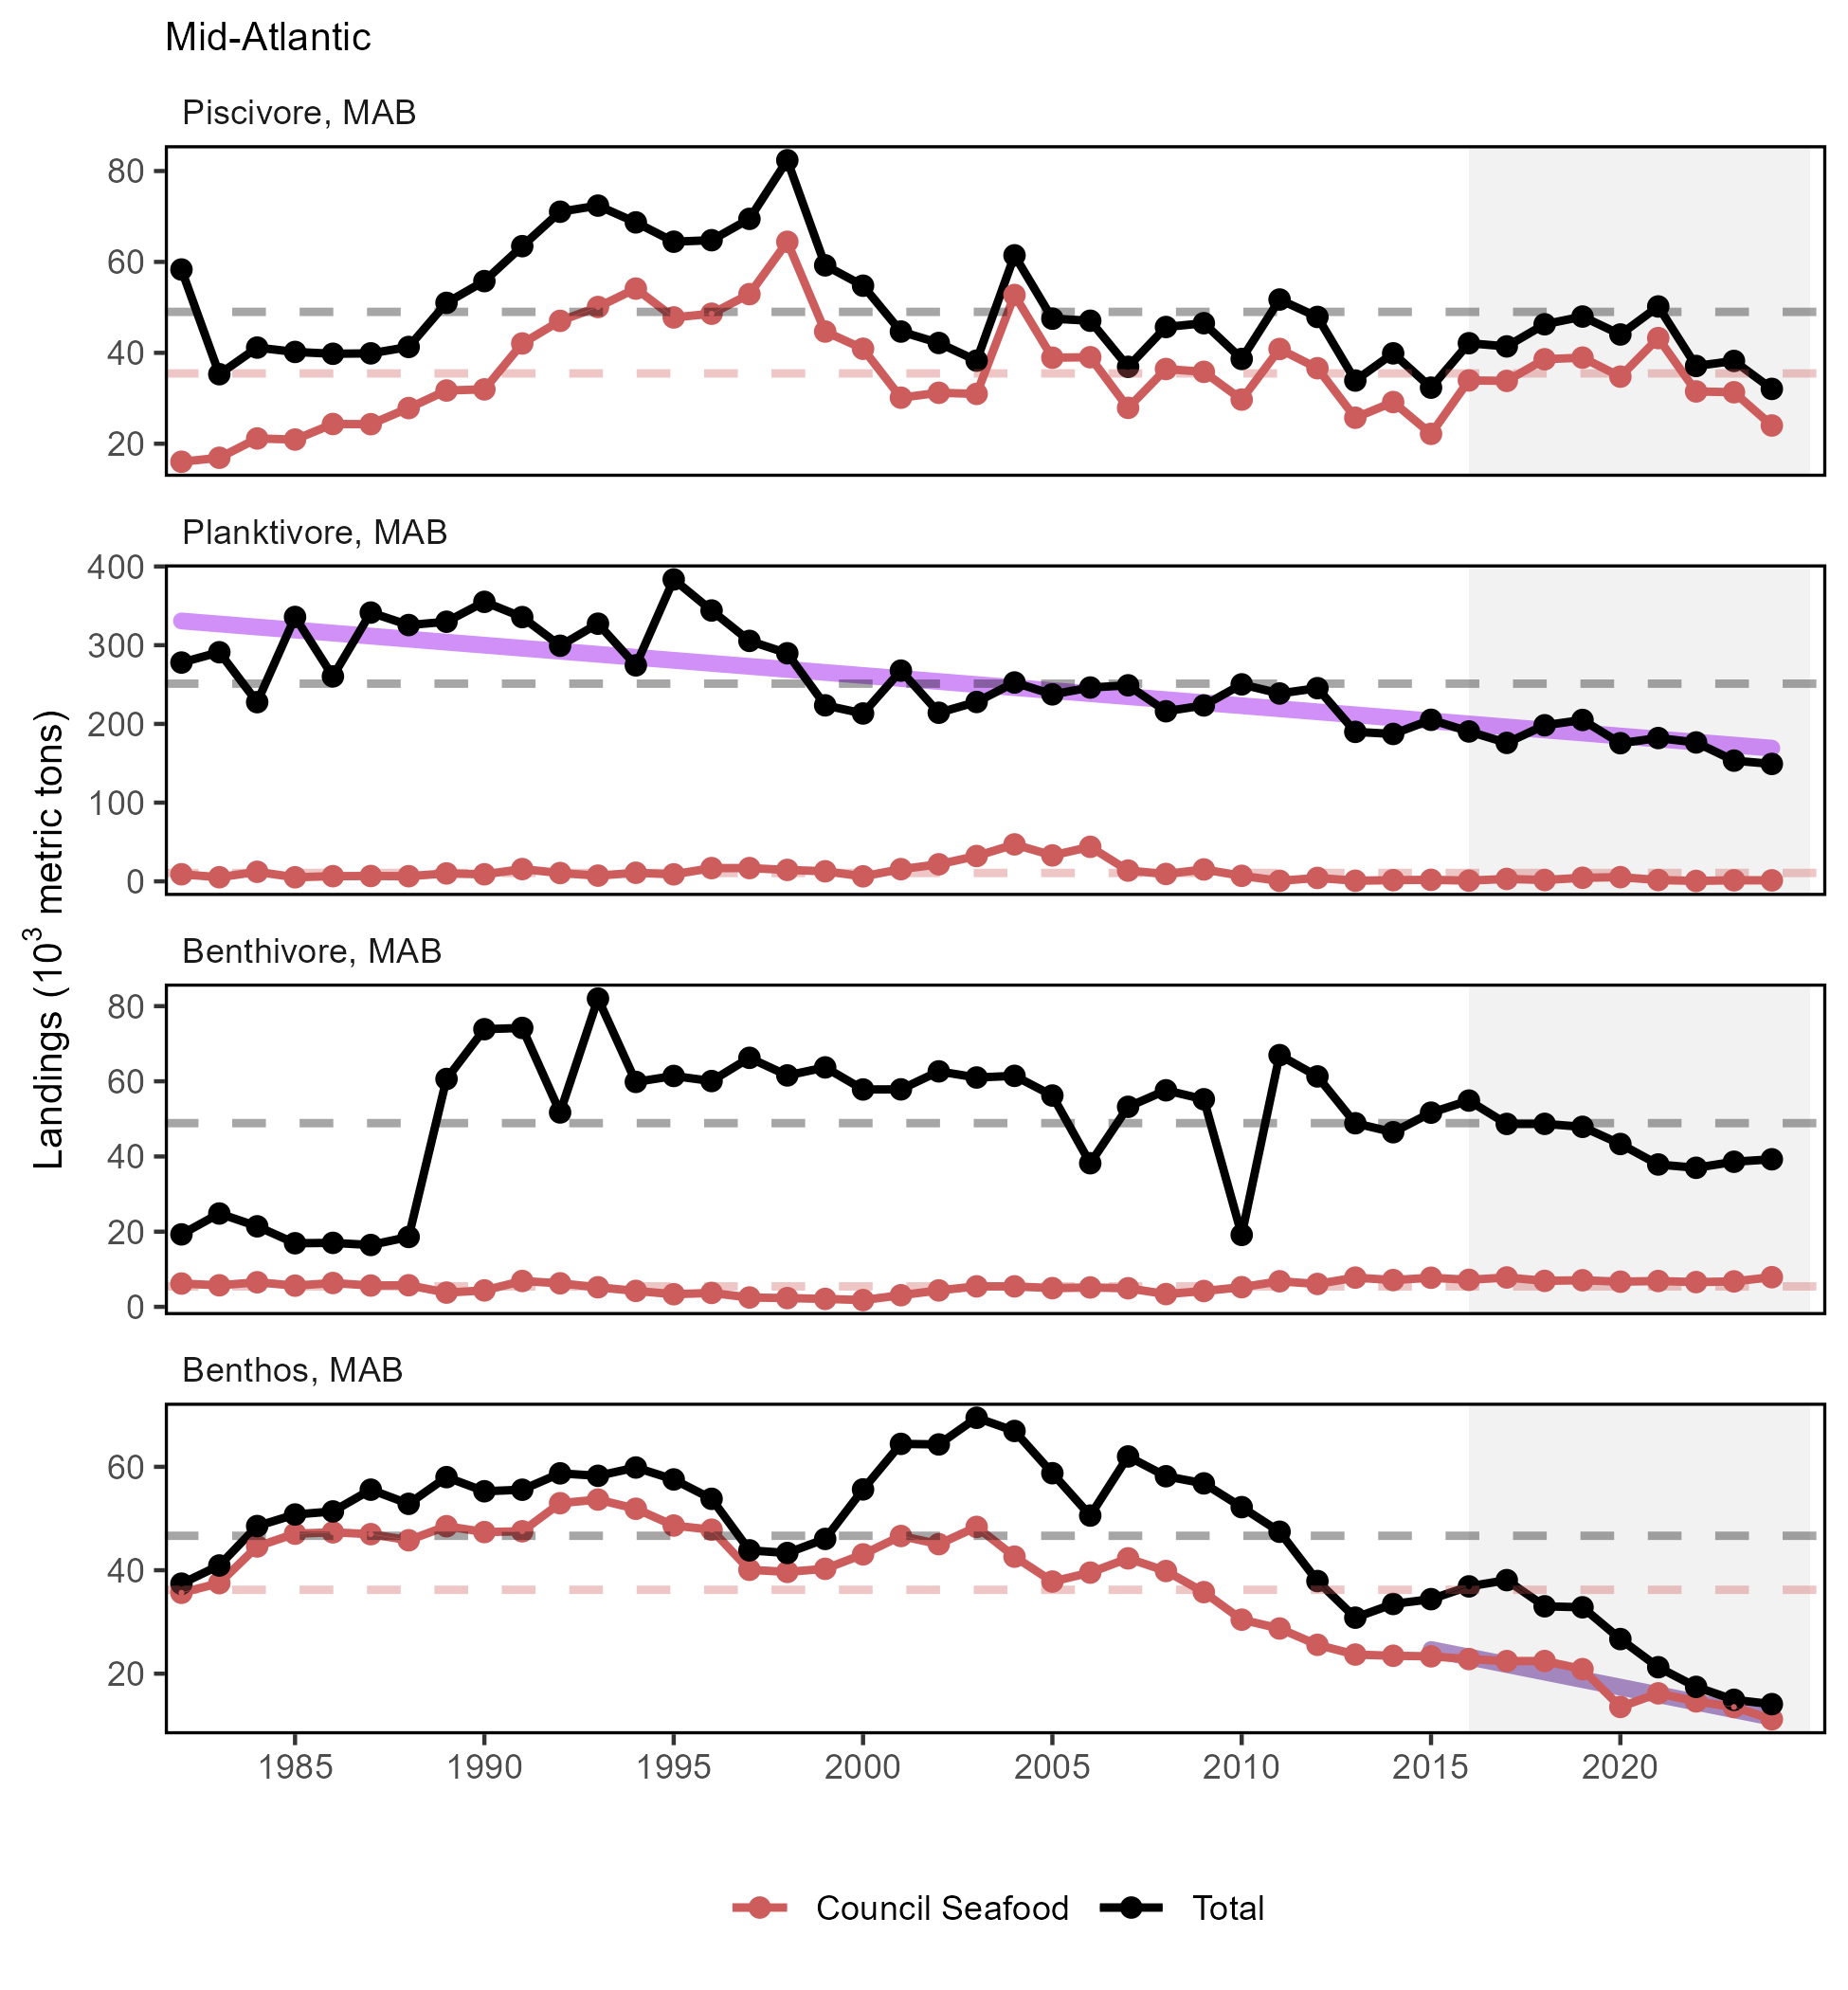
\includegraphics[width=1\linewidth,]{images/MidAtlantic/commercial_landings_MidAtlantic_2026-03-26} 

}

\caption{Total commercial landings in the Mid-Atlantic Bight (black) and Mid-Atlantic Fishery Management Council-managed U.S seafood landings (red) by feeding guild, with significant long-term declines (purple) in total planktivore landings and short-term declines (dark purple) in benthos landings.}\label{fig:comm-landings}
\end{figure}

Mid-Atlantic ports face a moderate to high risk from environmental variability, as evaluated by the 2025 \href{https://noaa-edab.github.io/catalog/community_climate_vulnerability.html}{Community Environmental Variability Risk Indicators} (Fig. \ref{fig:climatevul-land}). These \hyperref[community-social-and-climate-vulnerability]{indicators} assess port level risk to environmental variability based on dependence on species and their respective bioenvironmental vulnerabilities as assessed by regional experts. Total Vulnerability measures how much a region's landings (or revenue) is dependent on species that are sensitive to different climate and environmental change factors including temperature and acidification.

\begin{figure}[T]

{\centering 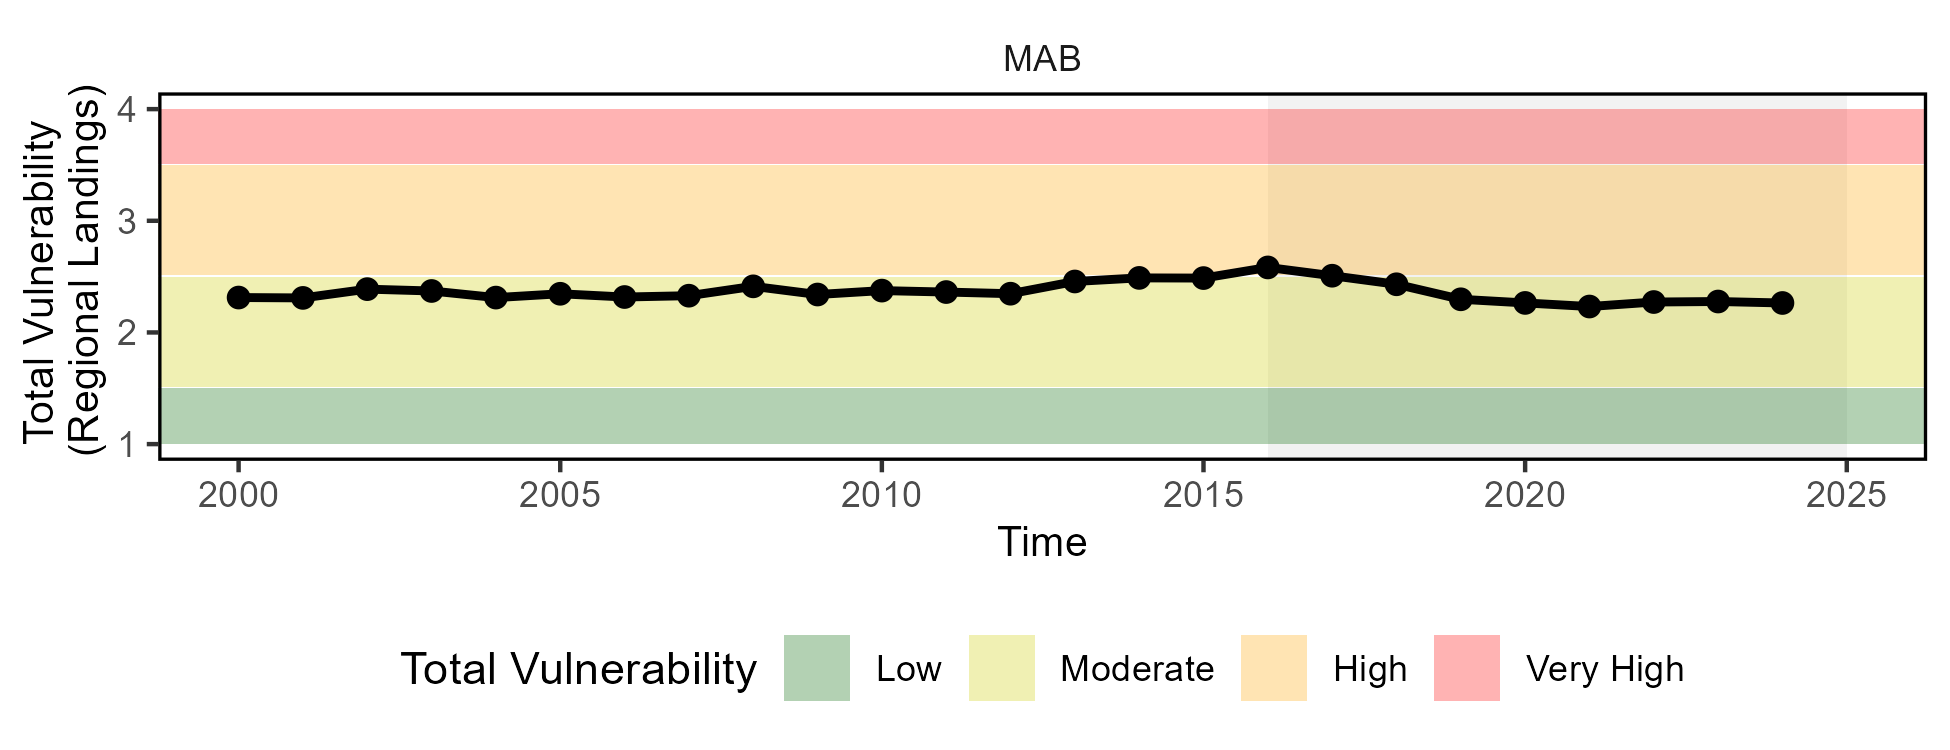
\includegraphics[width=1\linewidth,]{images/MidAtlantic/climatevul_land_MidAtlantic_2026-03-26} 

}

\caption{Mid-Atlantic region Total Vulnerability of commercial landings (sum of Mid-Atlantic port landings weighted by species vulnerability scores). Horizontal colored bars show different environmental variability risk levels. }\label{fig:climatevul-land}
\end{figure}

In the Mid-Atlantic, total \href{https://noaa-edab.github.io/catalog/recdat.html}{recreational harvest} (retained fish presumed to be eaten) shows a long-term decline with recent harvest remaining near a time series low (Fig. \ref{fig:rec-landings}). This pattern may indicate a shift towards catch-and-release strategies as opposed to catch for harvest. \href{https://noaa-edab.github.io/catalog/rec_hms.html}{Recreational shark landings} have generally decreased for most shark groups through 2024 (Fig \ref{fig:rec-hms}). The recent low in pelagic shark landings is largely driven by regulatory changes implemented in 2018, followed by the closure of the shortfin mako fishery in 2022. These actions were intended to rebuild the North Atlantic shortfin mako stock and comply with binding recommendations by the International Commission for the Conservation of Atlantic Tunas (ICCAT).

\begin{figure}[T]

{\centering 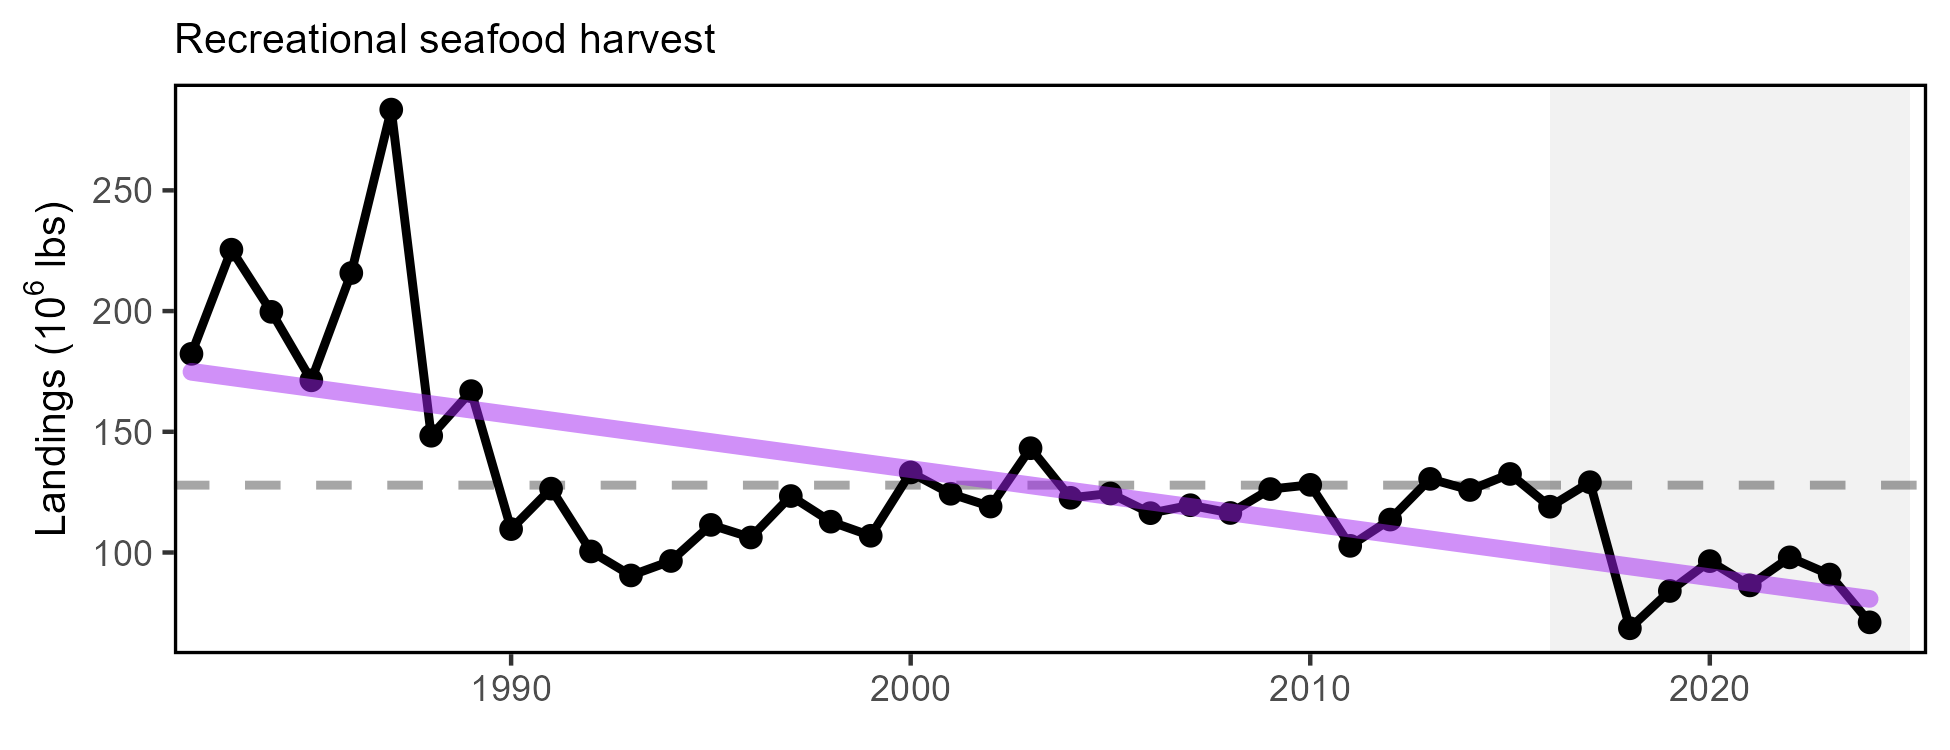
\includegraphics[width=1\linewidth,]{images/MidAtlantic/rec_landings_MidAtlantic_2026-03-26} 

}

\caption{Total recreational seafood harvest (millions of pounds, black, long-term significant decrease, purple) in the Mid-Atlantic region.}\label{fig:rec-landings}
\end{figure}

\begin{figure}[T]

{\centering 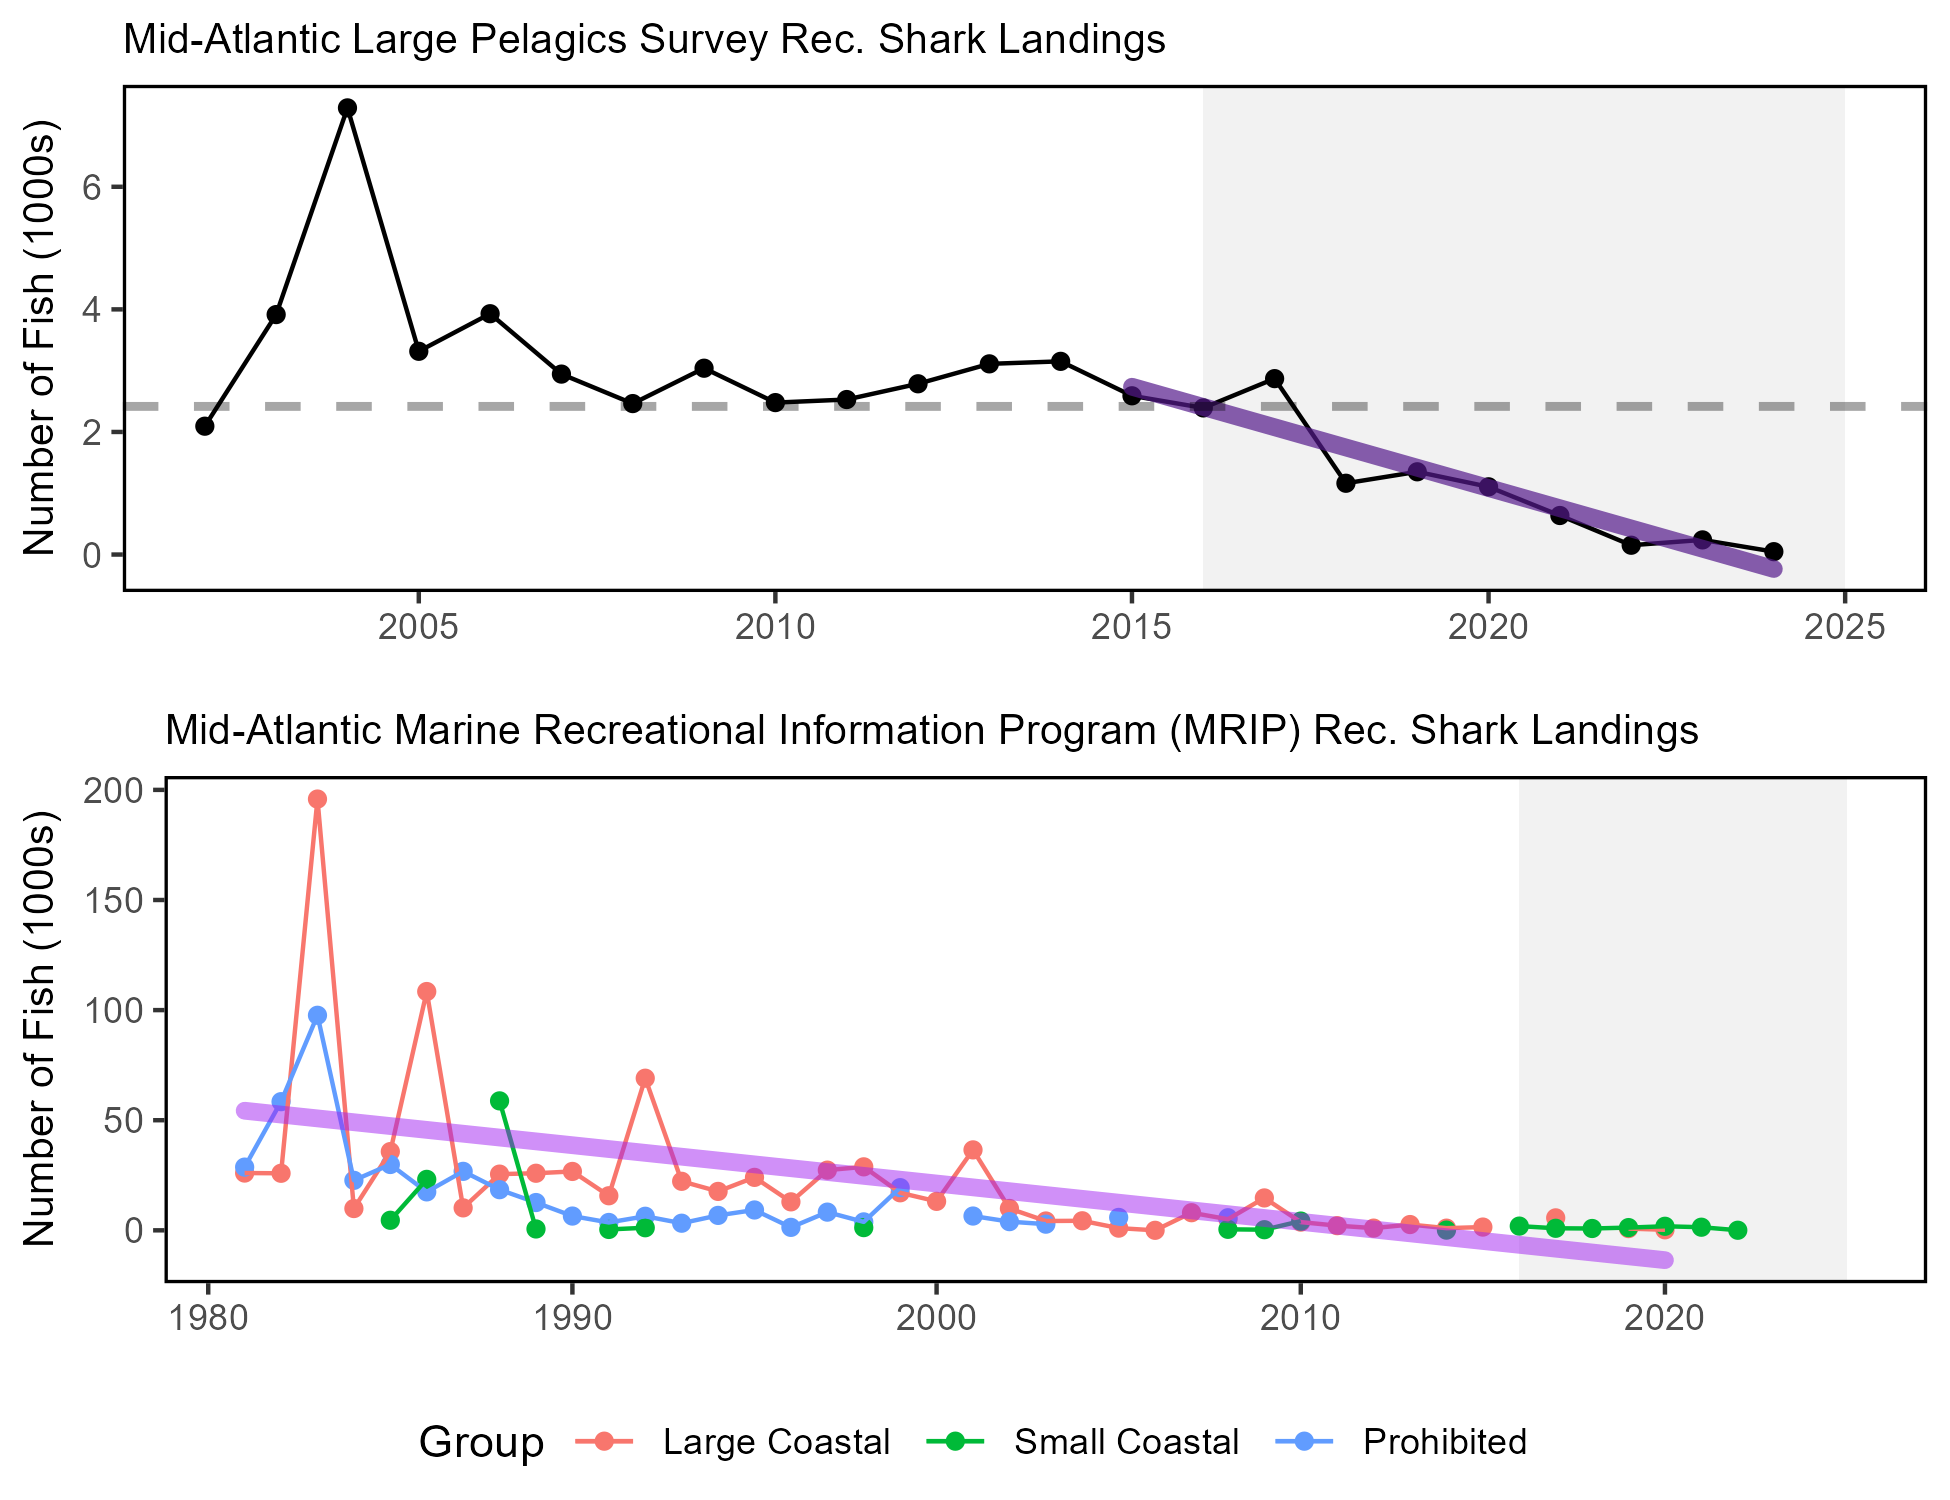
\includegraphics[width=1\linewidth,]{images/MidAtlantic/rec_hms_MidAtlantic_2026-03-26} 

}

\caption{Recreational shark landings in the Mid-Atlantic region from NOAA Fisheries Large Pelagics Survey (top, with short-term sigificant decline in dark purple) and Marine Recreational Information Program (MRIP, bottom) with long-term declining trend (purple). Note that the trend line is associated with the Large Coastal group, which has had no reported MRIP landings after 2020.}\label{fig:rec-hms}
\end{figure}

\href{https://noaa-edab.github.io/catalog/aquaculture.html?q=aqua\#aquaculture}{Aquaculture} can comprise a significant proportion of seafood production in specific communities, but not all aquaculture production is included in total seafood landings above. In 2022, the Northeast region produced approximately 6,300 metric tons of aquacultured shellfish, with revenue of \$133 million.

\subsubsection{Implications}\label{implications}

Declining commercial landings (total and seafood) and recreational harvest can be attributed to many interacting factors, including combinations of ecosystem and stock production, management actions, market conditions, and environmental change. While we cannot evaluate all possible drivers at present, here we evaluate the extent to which stock status, management, and system biomass trends may play a role.

\paragraph{Stock Status and Catch Limits}\label{stock-status-and-catch-limits}

Single species \href{https://noaa-edab.github.io/catalog/stock_status.html}{management objectives} (1. maintaining biomass above minimum thresholds and 2. maintaining fishing mortality below overfishing limits) are being met for all but two MAFMC-managed species (golden tilefish and Atlantic mackerel) (Fig. \ref{fig:stock-status}). However, the status of 5 stocks is unknown (northern shortfin squid, goosefish GOM/GB, goosefish southern GB/MAB, blueline tilefish, and chub mackerel), and longfin squid does not have an \(F/F_{MSY}\) estimate.

\begin{figure}[T]

{\centering 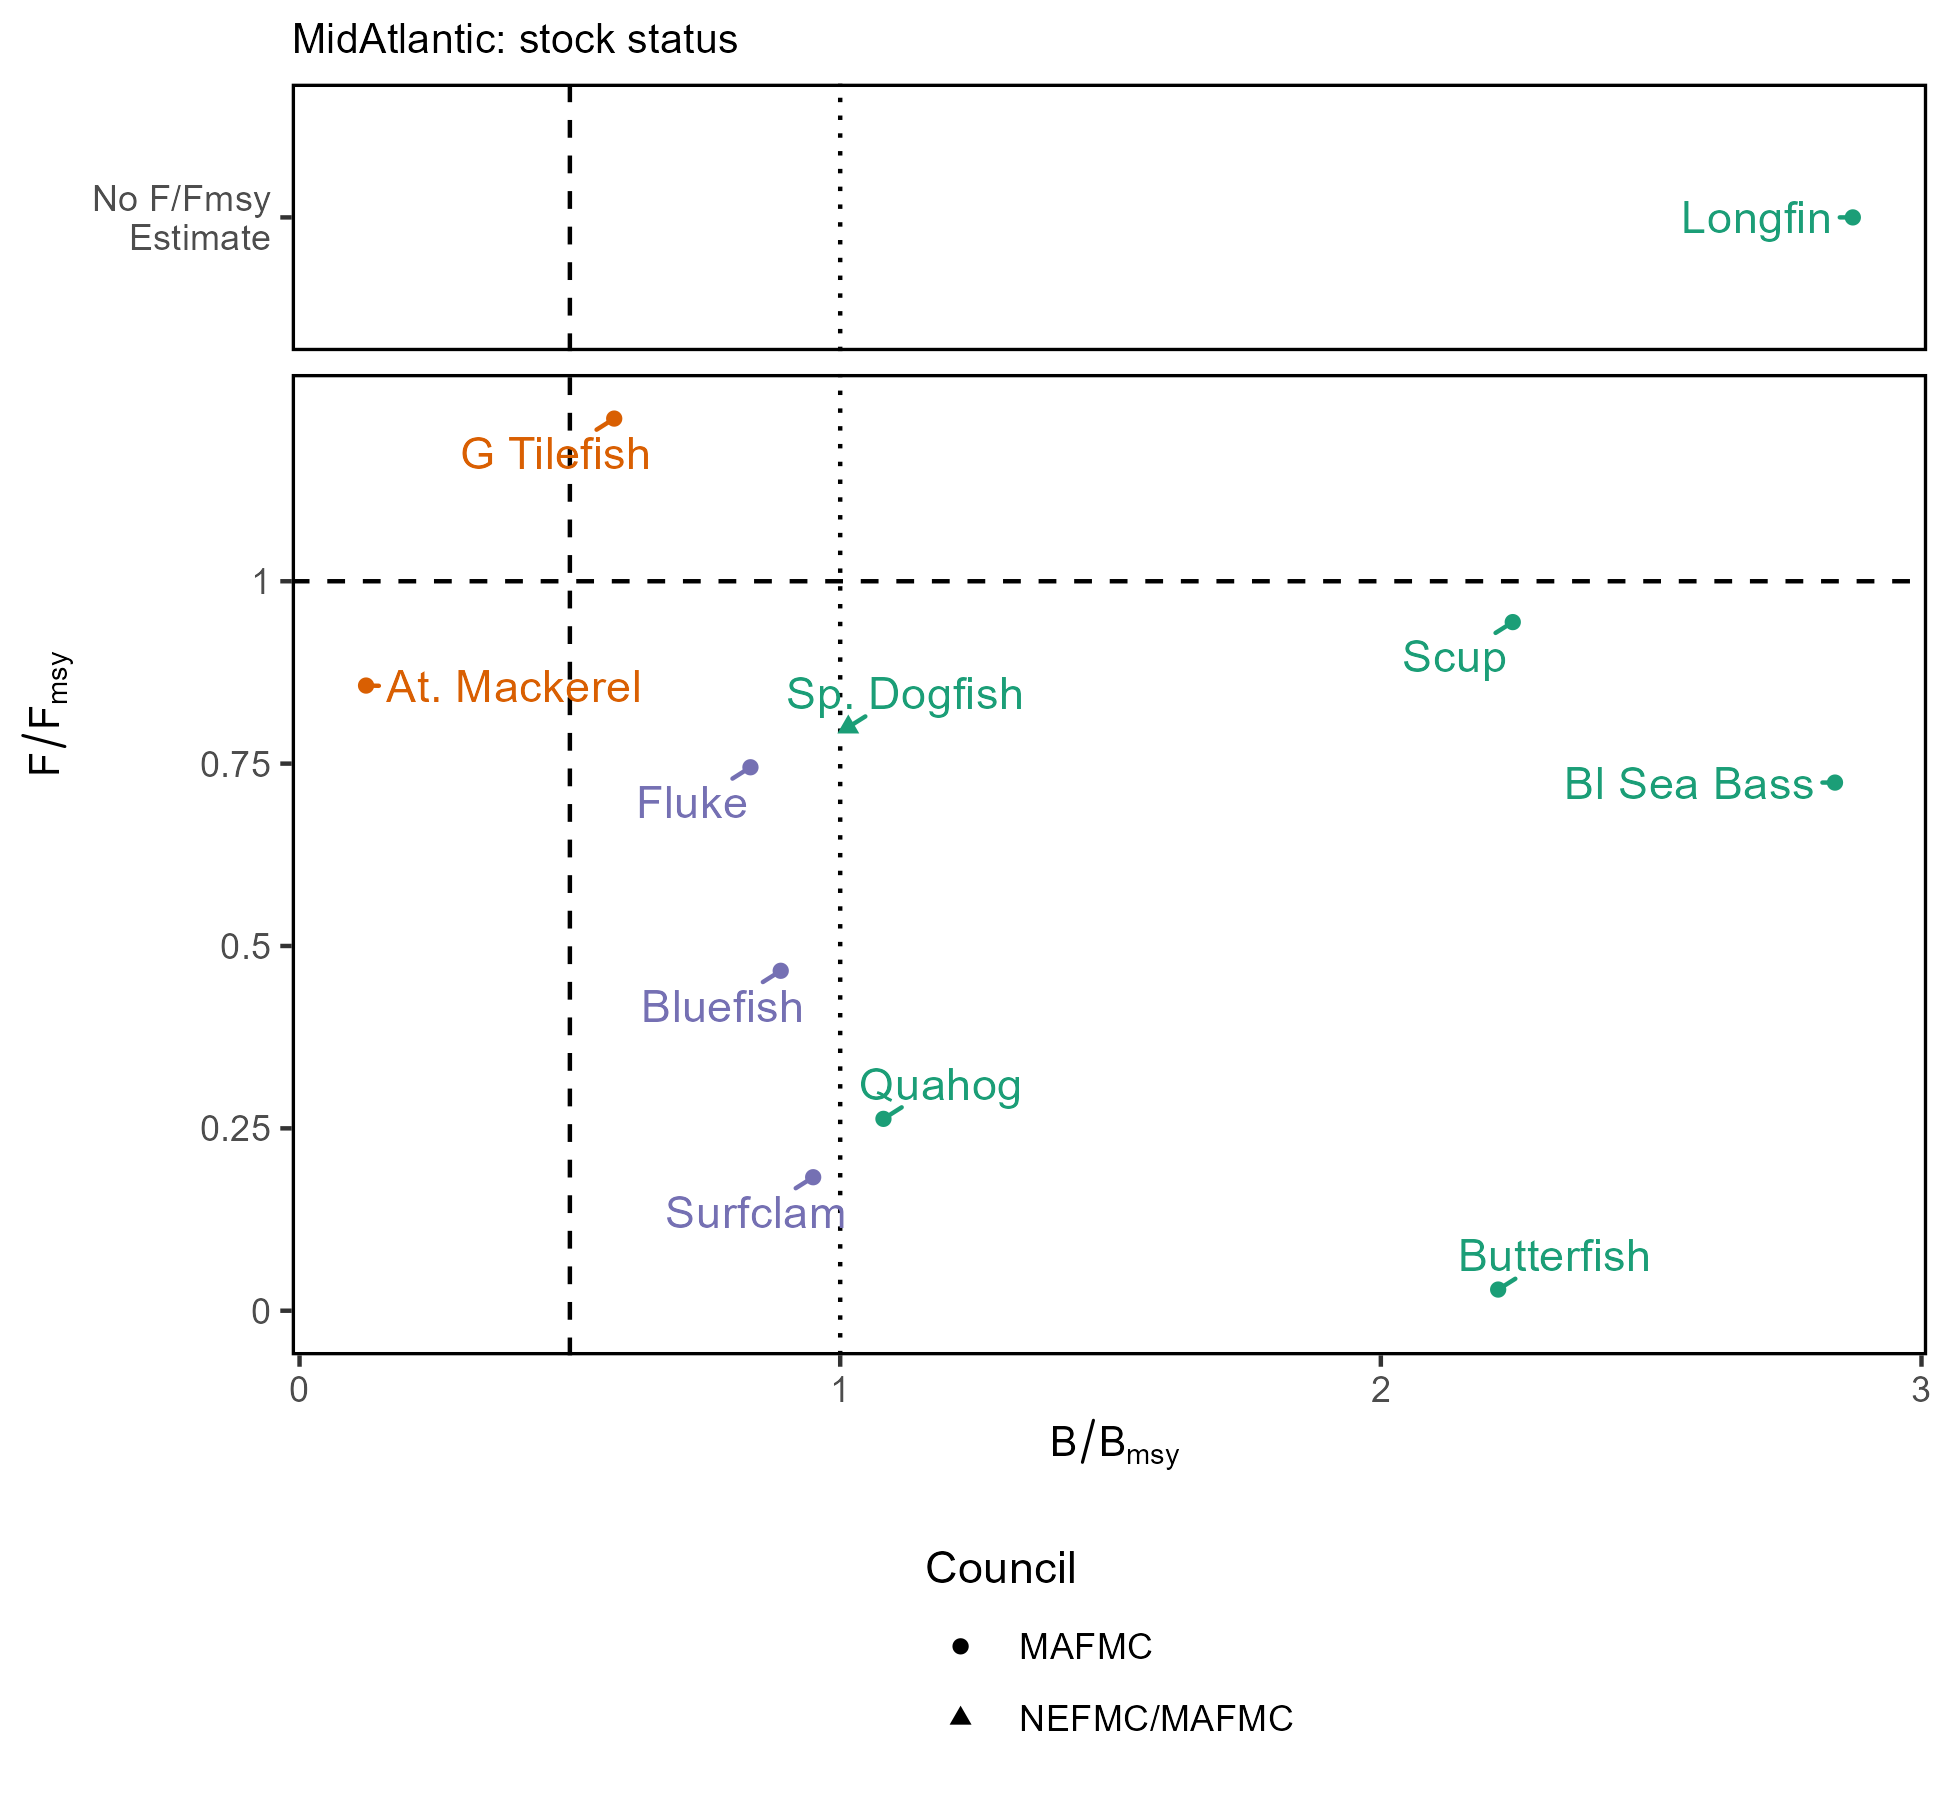
\includegraphics[width=1\linewidth,]{images/MidAtlantic/stock_status_MidAtlantic_2026-03-26} 

}

\caption{Summary of single species status for Mid-Atlantic Fishery Management Council and jointly federally managed stocks (spiny dogfish; goosefish has unknown status). The dotted vertical line is the target biomass reference point of $B_{MSY}$. The dashed lines are the management thresholds of one half $B_{MSY}$ (vertical) or $F_{MSY}$ (horizontal).  Stocks with a $B/B_{MSY}$ estimate but without an $F/F_{MSY}$ estimate are denoted in a separate box plot (top).  Colors denote stocks with $B/B_{MSY}$ < 0.5 or $F/F_{MSY}$>1 (orange), stocks 0.5<$B/B_{MSY}$<1 (blue), and stocks $B/B_{MSY}$>1 (green).}\label{fig:stock-status}
\end{figure}

Stock status and associated management constraints are unlikely to be driving decreased landings for some species, including quahog, surfclam, and northern shortfin squid. Most stocks are not fully utilizing their associated ABC or ACL, which includes landings and discards (Fig. \ref{fig:abcacl-stacked})(Fig. \ref{fig:abcacl-catch}). Quahog, surfclam, and northern shortfin squid have the largest ABC or ACLs but have low catch ratios, with less than 24\% of ABC or ACL caught in 2024. All other species except chub mackerel and longfin squid have catch ratios over 80\%, indicating that stock status and associated regulations are most likely constraining the landings of some species such as black sea bass, bluefish, and Atlantic mackerel. However, these management actions and regulations are enacted in response to biomass, such that less conservative regulations would not necessarily mean higher landings.

\begin{figure}[T]

{\centering 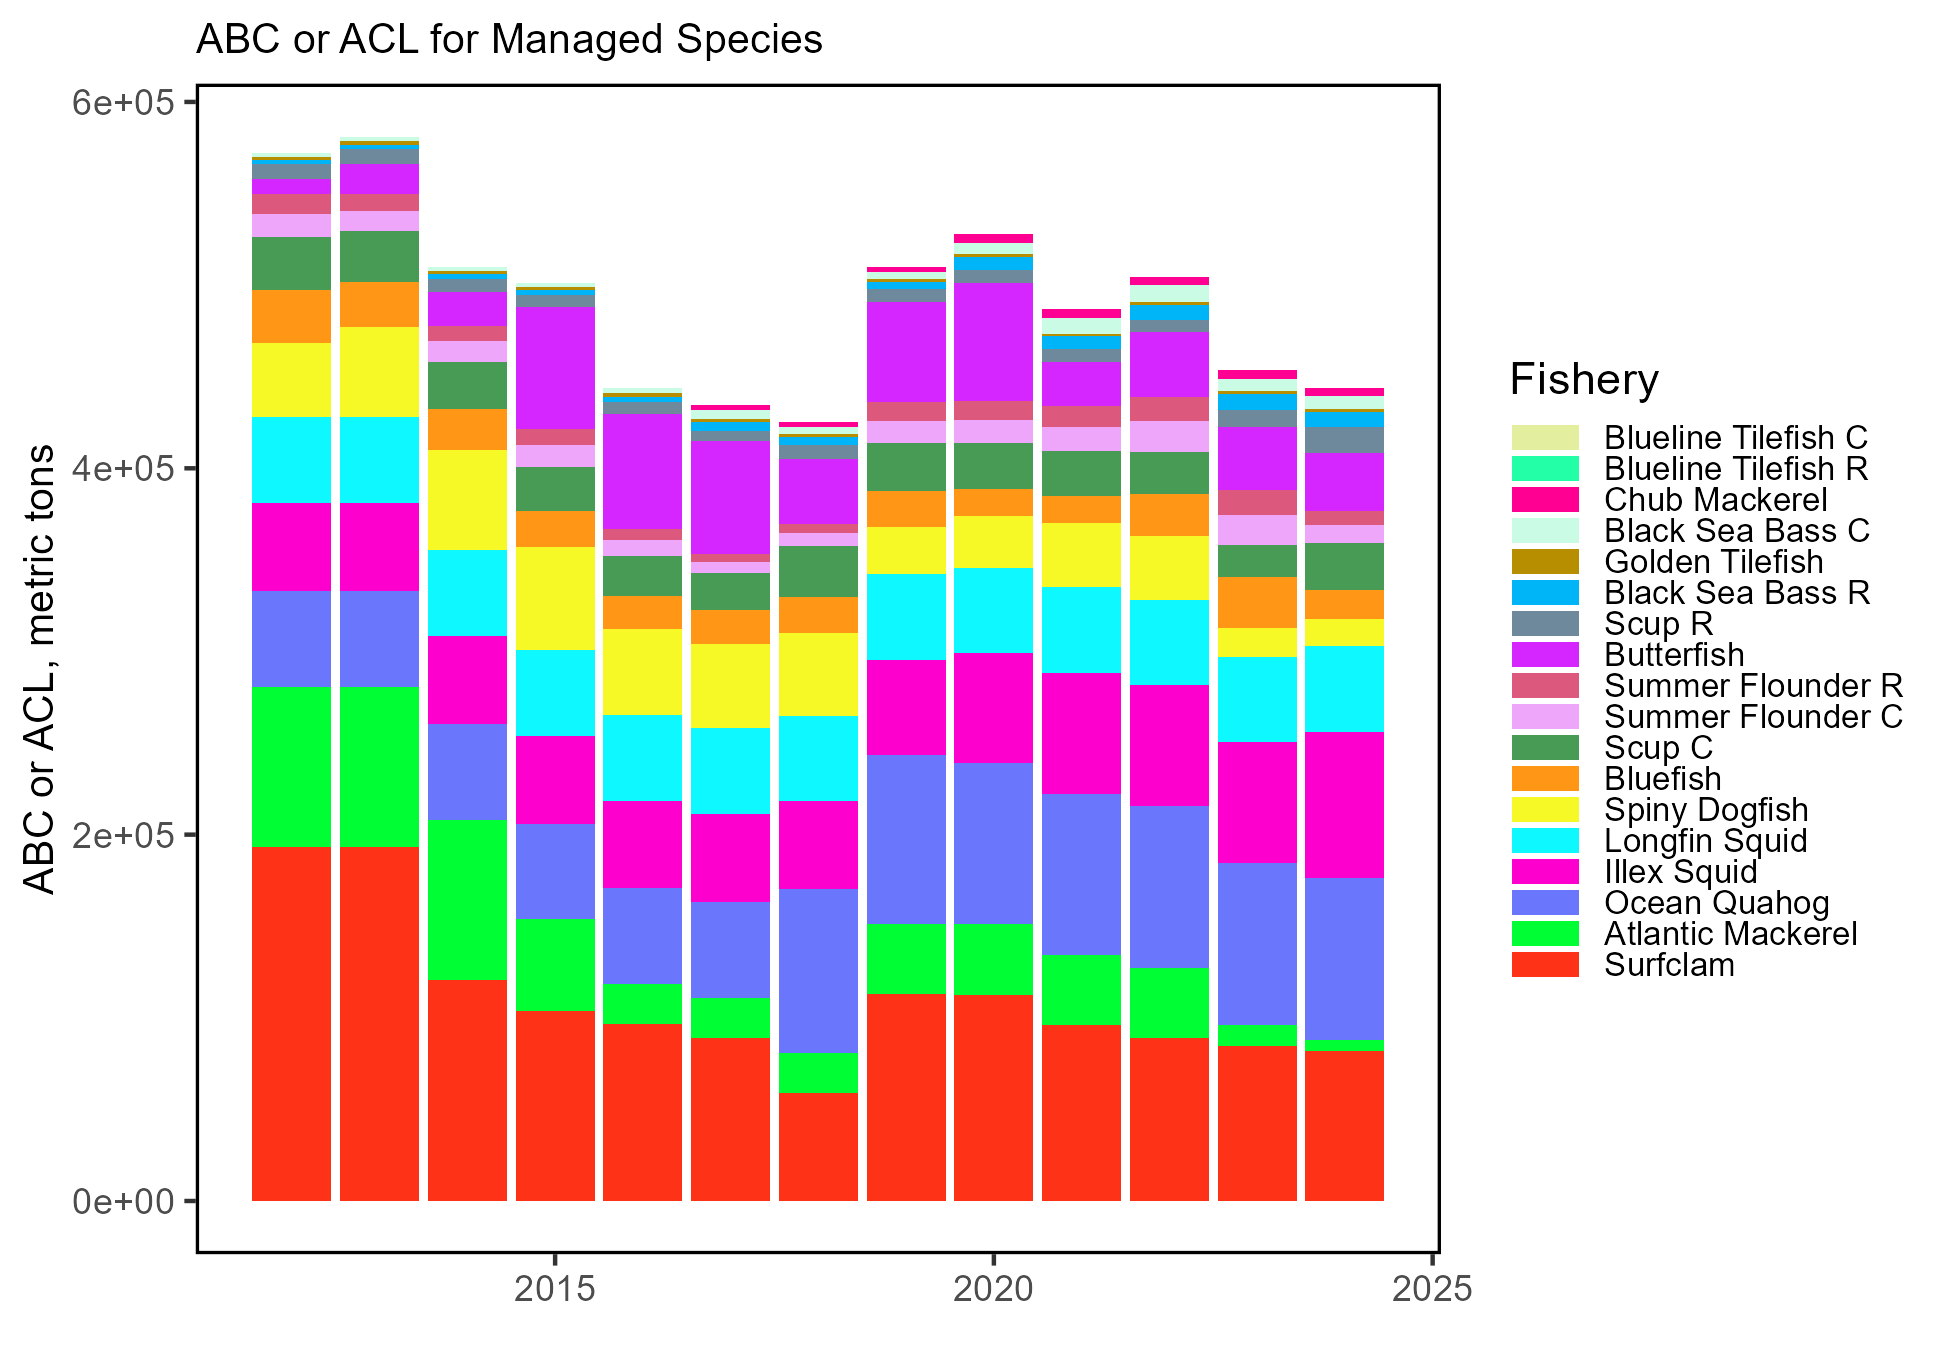
\includegraphics[width=1\linewidth,]{images/MidAtlantic/abcacl_stacked_MidAtlantic_2026-03-26} 

}

\caption{Sum of catch limits (in metric tons) across all Mid-Atlantic Fishery Management Council managed commercial (C) and recreational (R) fsheries.}\label{fig:abcacl-stacked}
\end{figure}

\begin{figure}[T]

{\centering 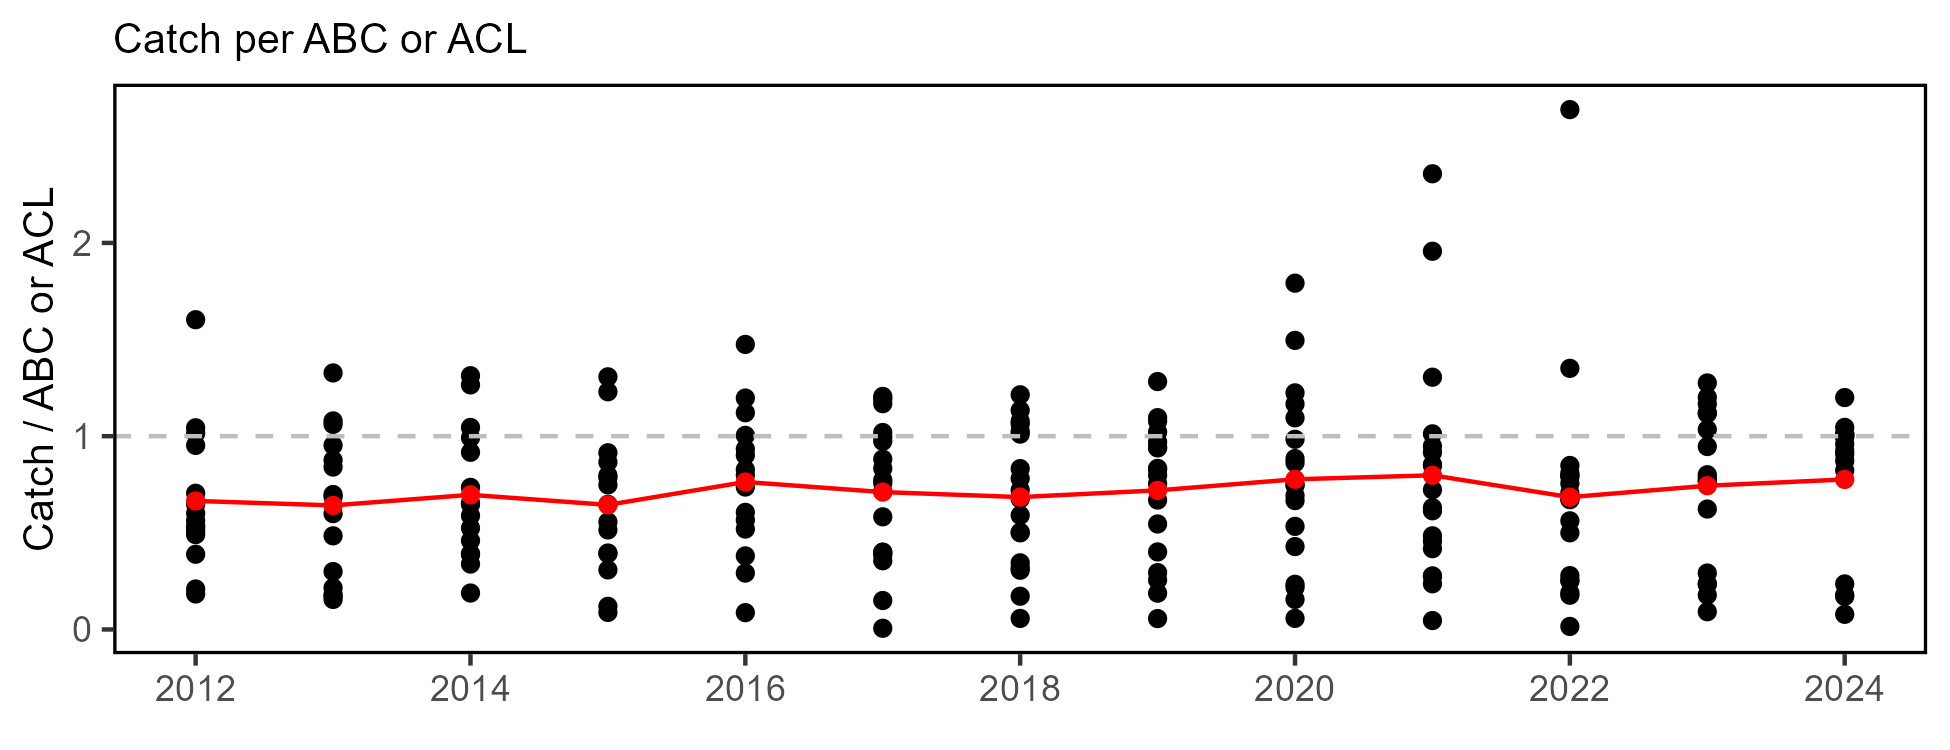
\includegraphics[width=1\linewidth,]{images/MidAtlantic/abcacl_catch_MidAtlantic_2026-03-26} 

}

\caption{Total catch divided by ABC/ACL for Mid-Atlantic Fishery Management Council managed fisheries. High points are recreational black sea bass (2021) and scup (2022). Red line indicates the median ratio across all fisheries.}\label{fig:abcacl-catch}
\end{figure}

\paragraph{System Biomass}\label{system-biomass}

Major shifts in feeding guilds or ecosystem trophic structure are unlikely to be driving the decline in landings. \href{https://noaa-edab.github.io/catalog/aggregate_biomass.html}{Aggregate biomass} trends derived from scientific resource surveys are mostly stable in the MAB, with long-term increases in spring piscivores, fall benthivores, and fall benthos (Fig. \ref{fig:nefsc-biomass-mab}). While managed species make up varying proportions of aggregate biomass, trends in landings are not mirroring shifts in the overall trophic structure of survey-sampled fish and invertebrates. Future study should investigate whether shifts in the relative abundance of targeted species may be playing a role.

\paragraph{Effect on Seafood Production}\label{effect-on-seafood-production}

Stock status is not likely driving declining seafood production in the MAB, as all but two stocks are above the minimum threshold, and aggregate biomass trends appear stable or increasing. The decline in managed commercial seafood landings of surfclams and quahogs is driven by a combination of population abundance, distribution changes, and market dynamics. Recent catch has been low relative to the quota for these species. The decrease in regional availability of scallops has contributed to the decline of benthos landings not managed by the MAFMC. The long-term declines in total and planktivore landings is driven in part by Atlantic menhaden fishery dynamics, including a consolidation of processors leading to reduced fishing capacity between the 1990s and mid-2000s.

Changes in the spatial distribution of surfclams and ocean quahogs may be constraining seafood production, as this results in areas with overlapping distributions and the potential for mixed landings. Mixed landings are currently prohibited by regulations, which could become problematic for harvesters. However, the MAFMC submitted an amendment in August 2025 to NOAA Fisheries to allow mixed surfclam and quahog trips; as of February 2026, the amendment remains under review by NOAA.

The recent decline in recreational seafood harvest is likely associated with a combination of targeted management actions, shifting social behaviors, and data collection changes. The decline in recreational shark landings can partially be attributed to management actions intended to reduce fishing mortality on mako sharks. The lower than average landings since 2018 for species other than sharks could be driven by either changes in fishing behavior or reflect the modified methodology in NOAA Fisheries' Marine Recreational Information Program survey in 2018.

Future commercial and recreational landings are likely to be driven by environmental changes that require continued monitoring. Overall, the majority of landings from Mid-Atlantic ports is increasingly dependent on species with moderate environmental vulnerability (Fig. \ref{fig:commvulex}). Fisheries and communities rely on different combinations of stocks, and individual stocks will respond differently to these drivers. Some key drivers include:

\begin{itemize}
\tightlist
\item
  \textbf{Unprecedented Climate Shifts}: Global ocean temperatures have reached record highs (see \hyperref[highlights]{2025 Highlights section}) and the Northeast US shelf has experienced long-term warming.
\item
  \textbf{Distribution Shifts}: Stocks are shifting towards the northeast and into deeper waters throughout the Northeast US Large Marine Ecosystem (see \hyperref[climate-and-ecosystem-change]{Climate Risks section}).
\item
  \textbf{Ecosystem production}: Changes in ecosystem composition and biological production are impacting the stability of the \hyperref[stability]{ecosystem} and pose \hyperref[risks-to-setting-catch-limits]{risks to setting catch limits}.
\item
  \textbf{Community Risks}: Changes in the ecosystem can affect the \hyperref[stability]{stability} of fisheries and pose \hyperref[community-social-and-climate-vulnerability]{risks to fishing communities}.
\end{itemize}

\begin{figure}[T]

{\centering 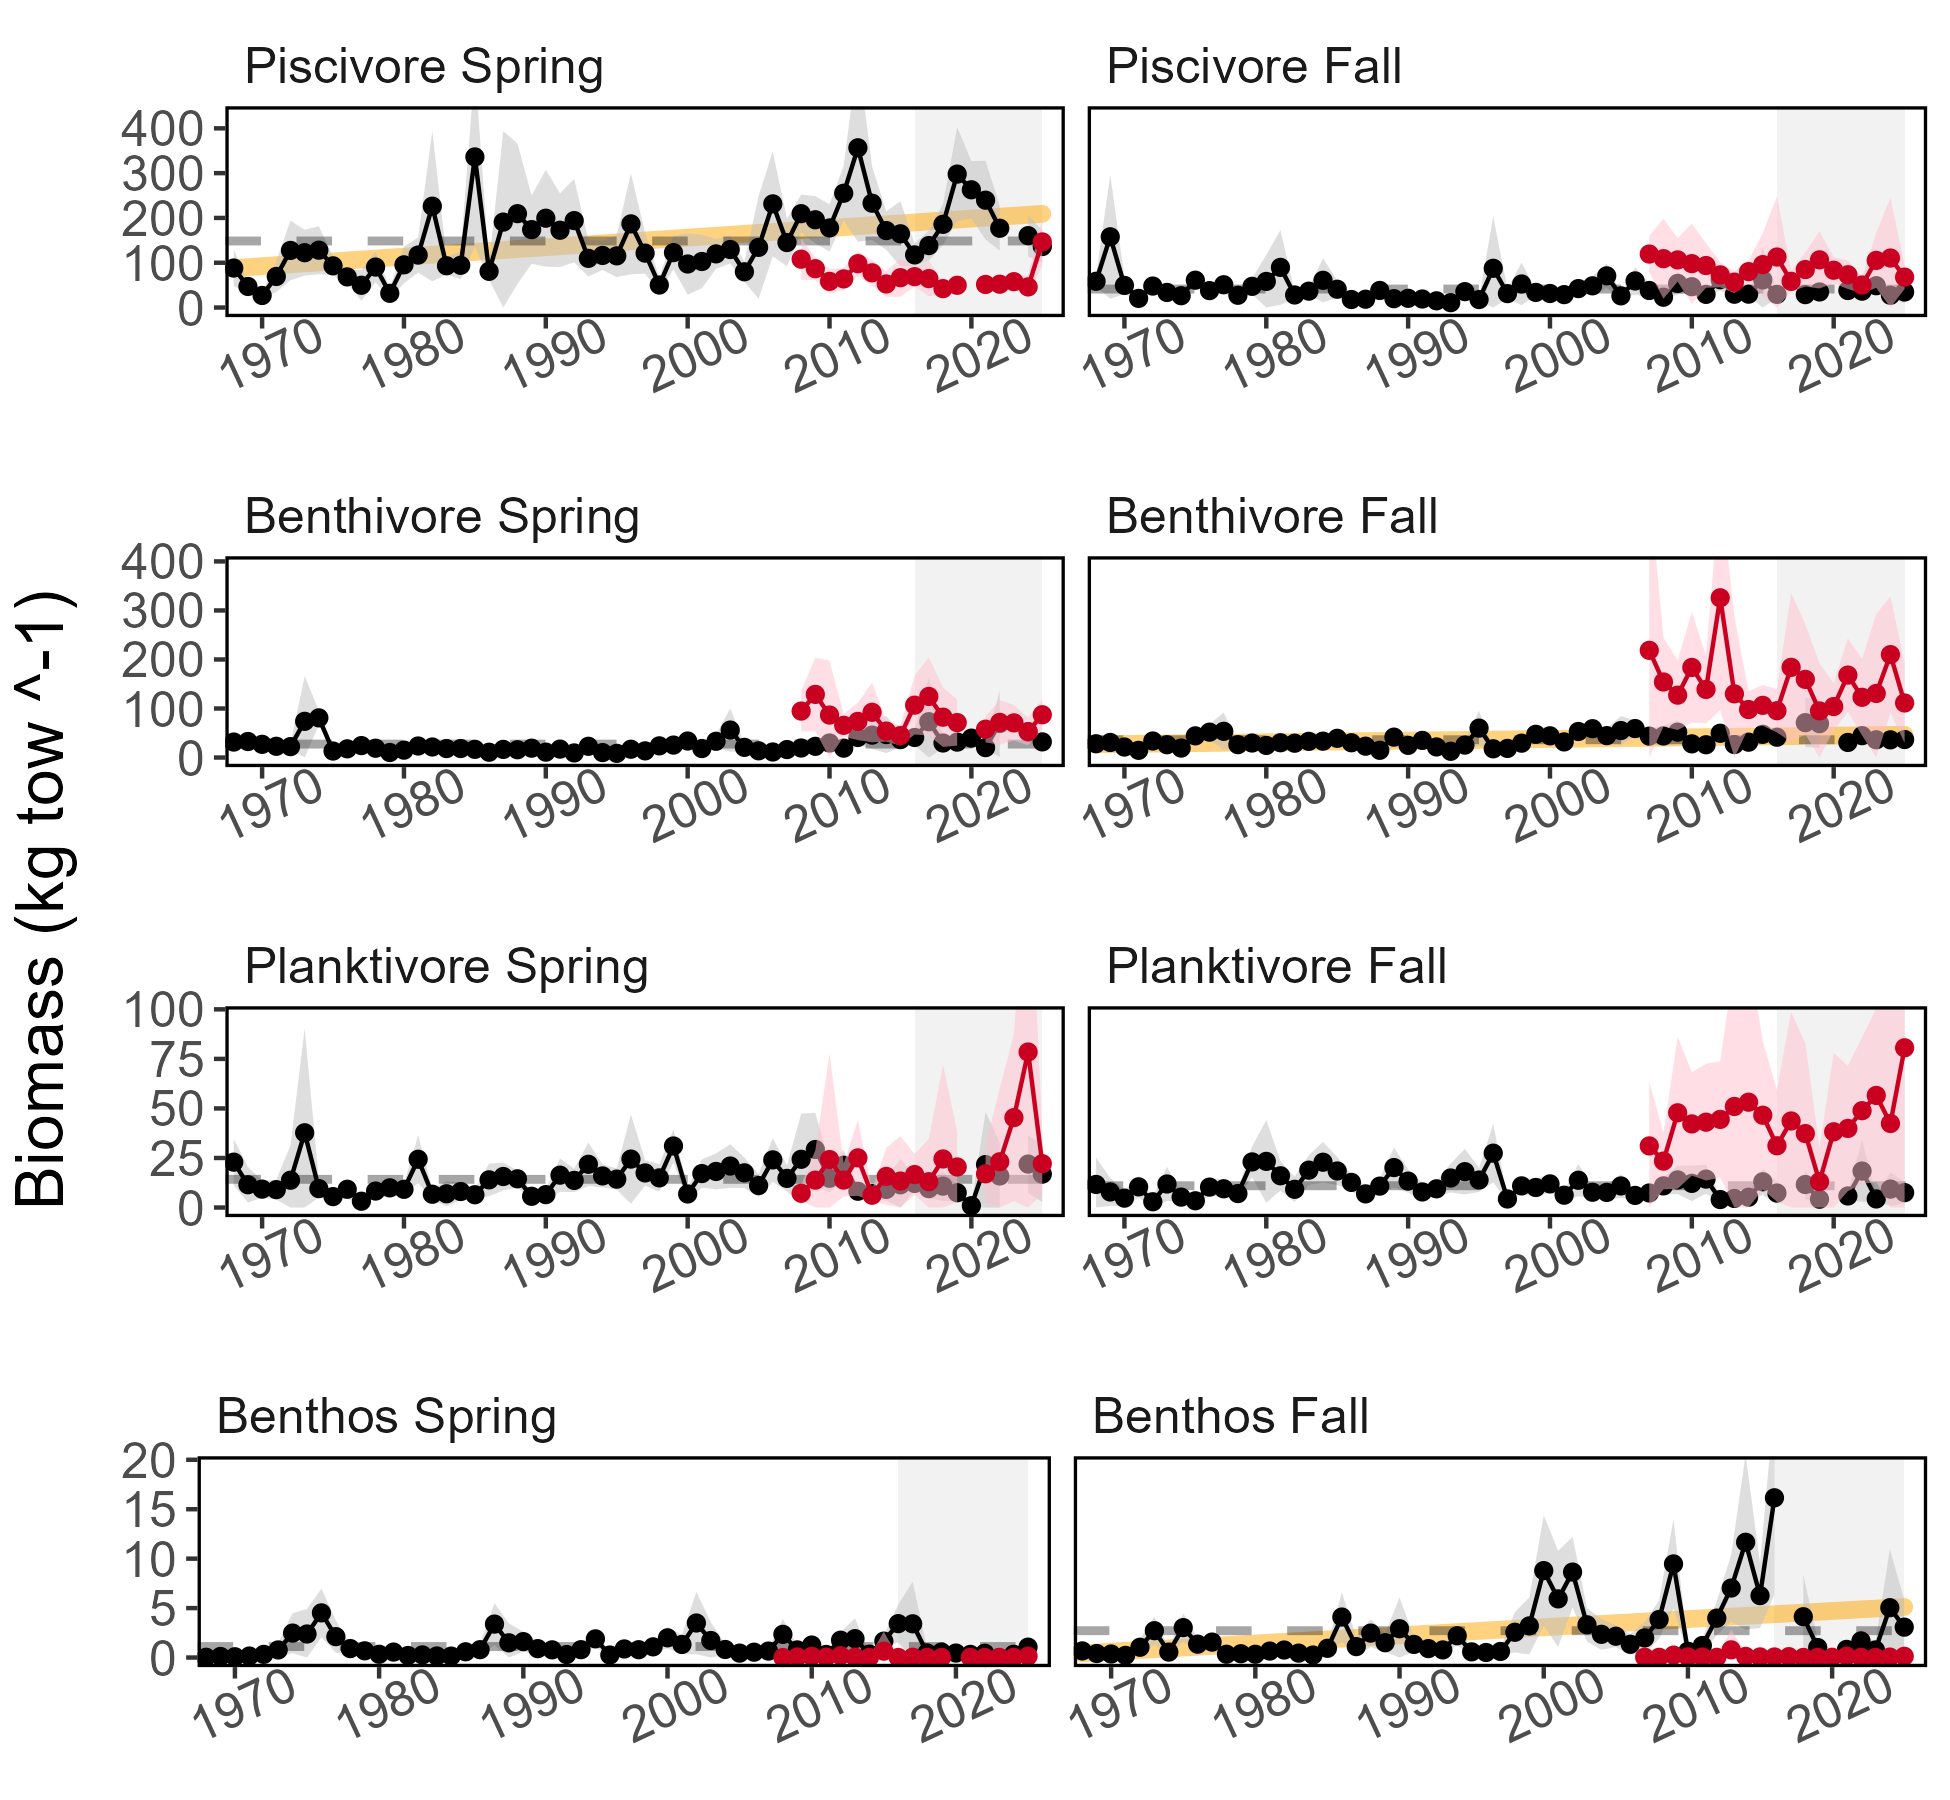
\includegraphics[width=1\linewidth,]{images/MidAtlantic/aggregate_biomass_mab_MidAtlantic_2026-03-26} 

}

\caption{Spring (left) and fall (right) surveyed biomass in the Mid-Atlantic Bight. Data from the Northeast Fisheries Science Center Bottom Trawl Survey are shown in black, with the nearshore Northeast Area Monitoring and Assessment Program (NEAMAP) survey shown in red. Long-term significant increases (orange lines) are present for spring piscivore, fall benthivore, and fall benthos biomass. The shaded area around each annual mean represents 2 standard deviations from the mean.}\label{fig:nefsc-biomass-mab}
\end{figure}

\newpage

\subsection{Commercial Profits}\label{commercial-profits}

\subsubsection{Indicators: revenue \& net revenue}\label{indicators-revenue-net-revenue}

Total \href{https://noaa-edab.github.io/catalog/comdat.html}{commercial revenue} and MAFMC managed species revenue (2024 USD) within the Mid-Atlantic Bight have declined over the past 20 years. In 2024, total revenue and MAFMC managed species revenue were both near an all-time low (Fig. \ref{fig:comm-revenue}).

\begin{figure}[T]

{\centering 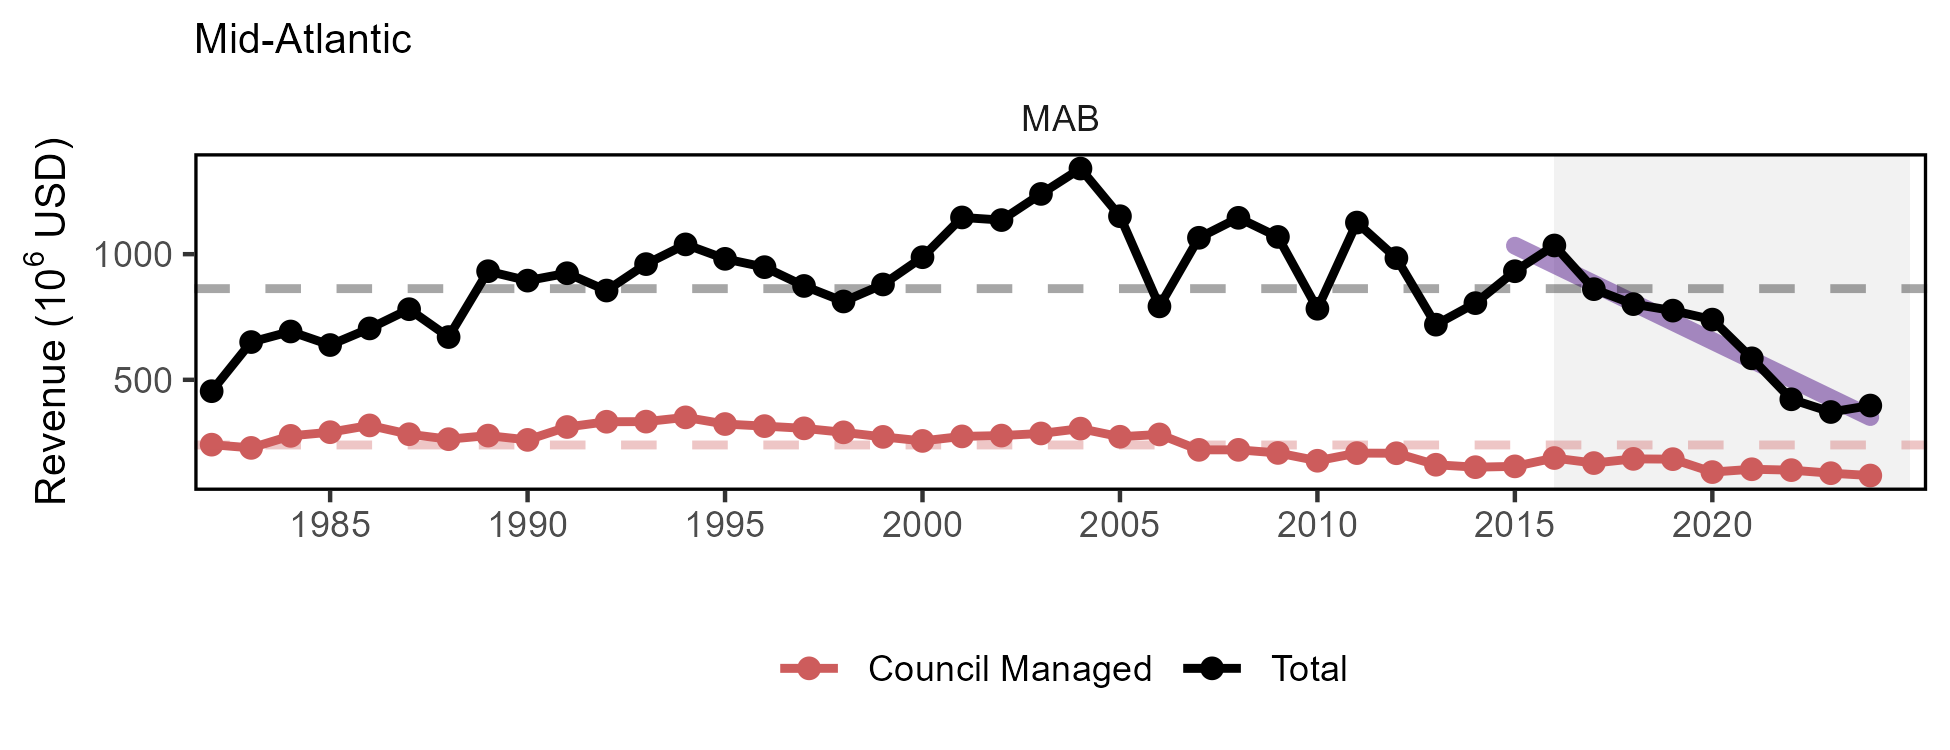
\includegraphics[width=1\linewidth,]{images/MidAtlantic/comm_revenue_MidAtlantic_2026-03-26} 

}

\caption{Commercial revenue (2024 USD) through 2024 for the Mid-Atlantic region: total (black) and from Mid-Atlantic Fishery Managment Councli managed species (red). Dashed lines represent the long-term annual mean. A short-term significant decrease is present for total revenue (purple).}\label{fig:comm-revenue}
\end{figure}

Revenue earned by harvesting resources is a function of both the quantity landed of each species and the prices paid for landings. Therefore, total revenue patterns can be driven by harvest levels, the mix of species landed, price changes, or a combination of these. The \href{https://noaa-edab.github.io/catalog/bennet.html}{Bennet Indicator} (BI) decomposes revenue change into two parts, one driven by changing quantities (volumes), and a second driven by changing prices. All changes are in relation to a base year (1982). The 1982 base year was selected because that is the first year the relevant data is available and it allows for an extended period of time to evaluate market trends and dynamics. The BI results demonstrate that relatively high revenues in 2014-2016 were somewhat equally due to higher landings and prices (Fig. \ref{fig:bennet}). In more recent years, both landings and prices have been closer to values from the reference year (1982). Low prices coupled with low volumes landed led to low revenue in 2024. Recent lower than baseline revenues are partially due to lower volumes and prices of benthos species (Fig. \ref{fig:bennet-all}).

\begin{figure}[T]

{\centering 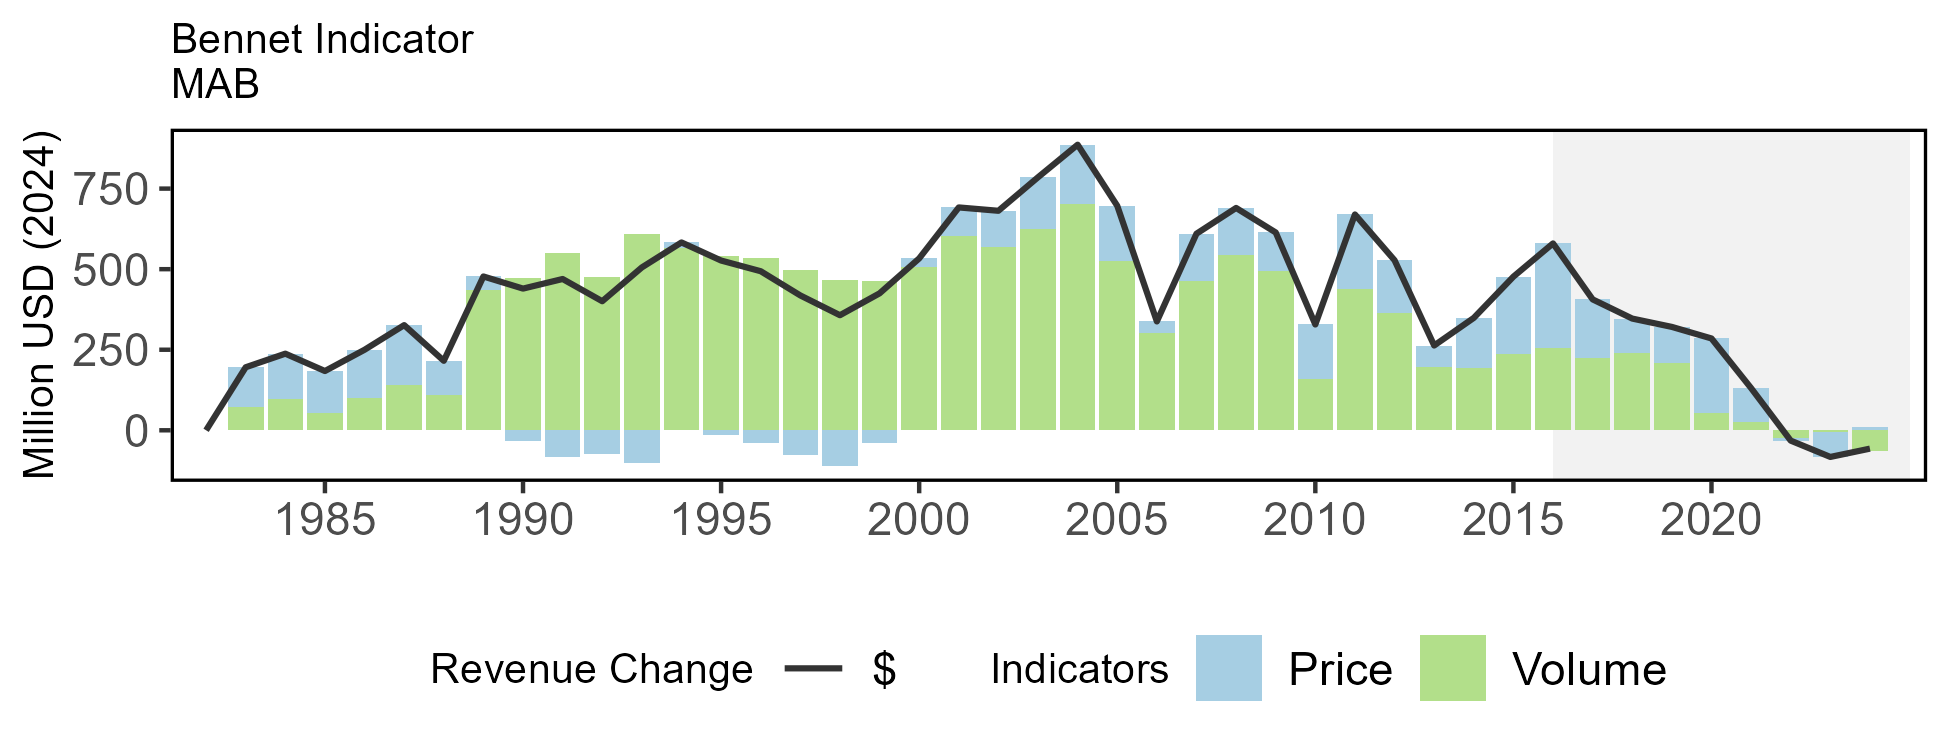
\includegraphics[width=1\linewidth,]{images/MidAtlantic/bennet_MidAtlantic_2026-03-26} 

}

\caption{Revenue change from 1982 values in 2024 dollars (black); Price (blue), and Volume Indicators (green) for total commercial landings in the Mid-Atlantic Bight.}\label{fig:bennet}
\end{figure}

\begin{figure}[T]

{\centering 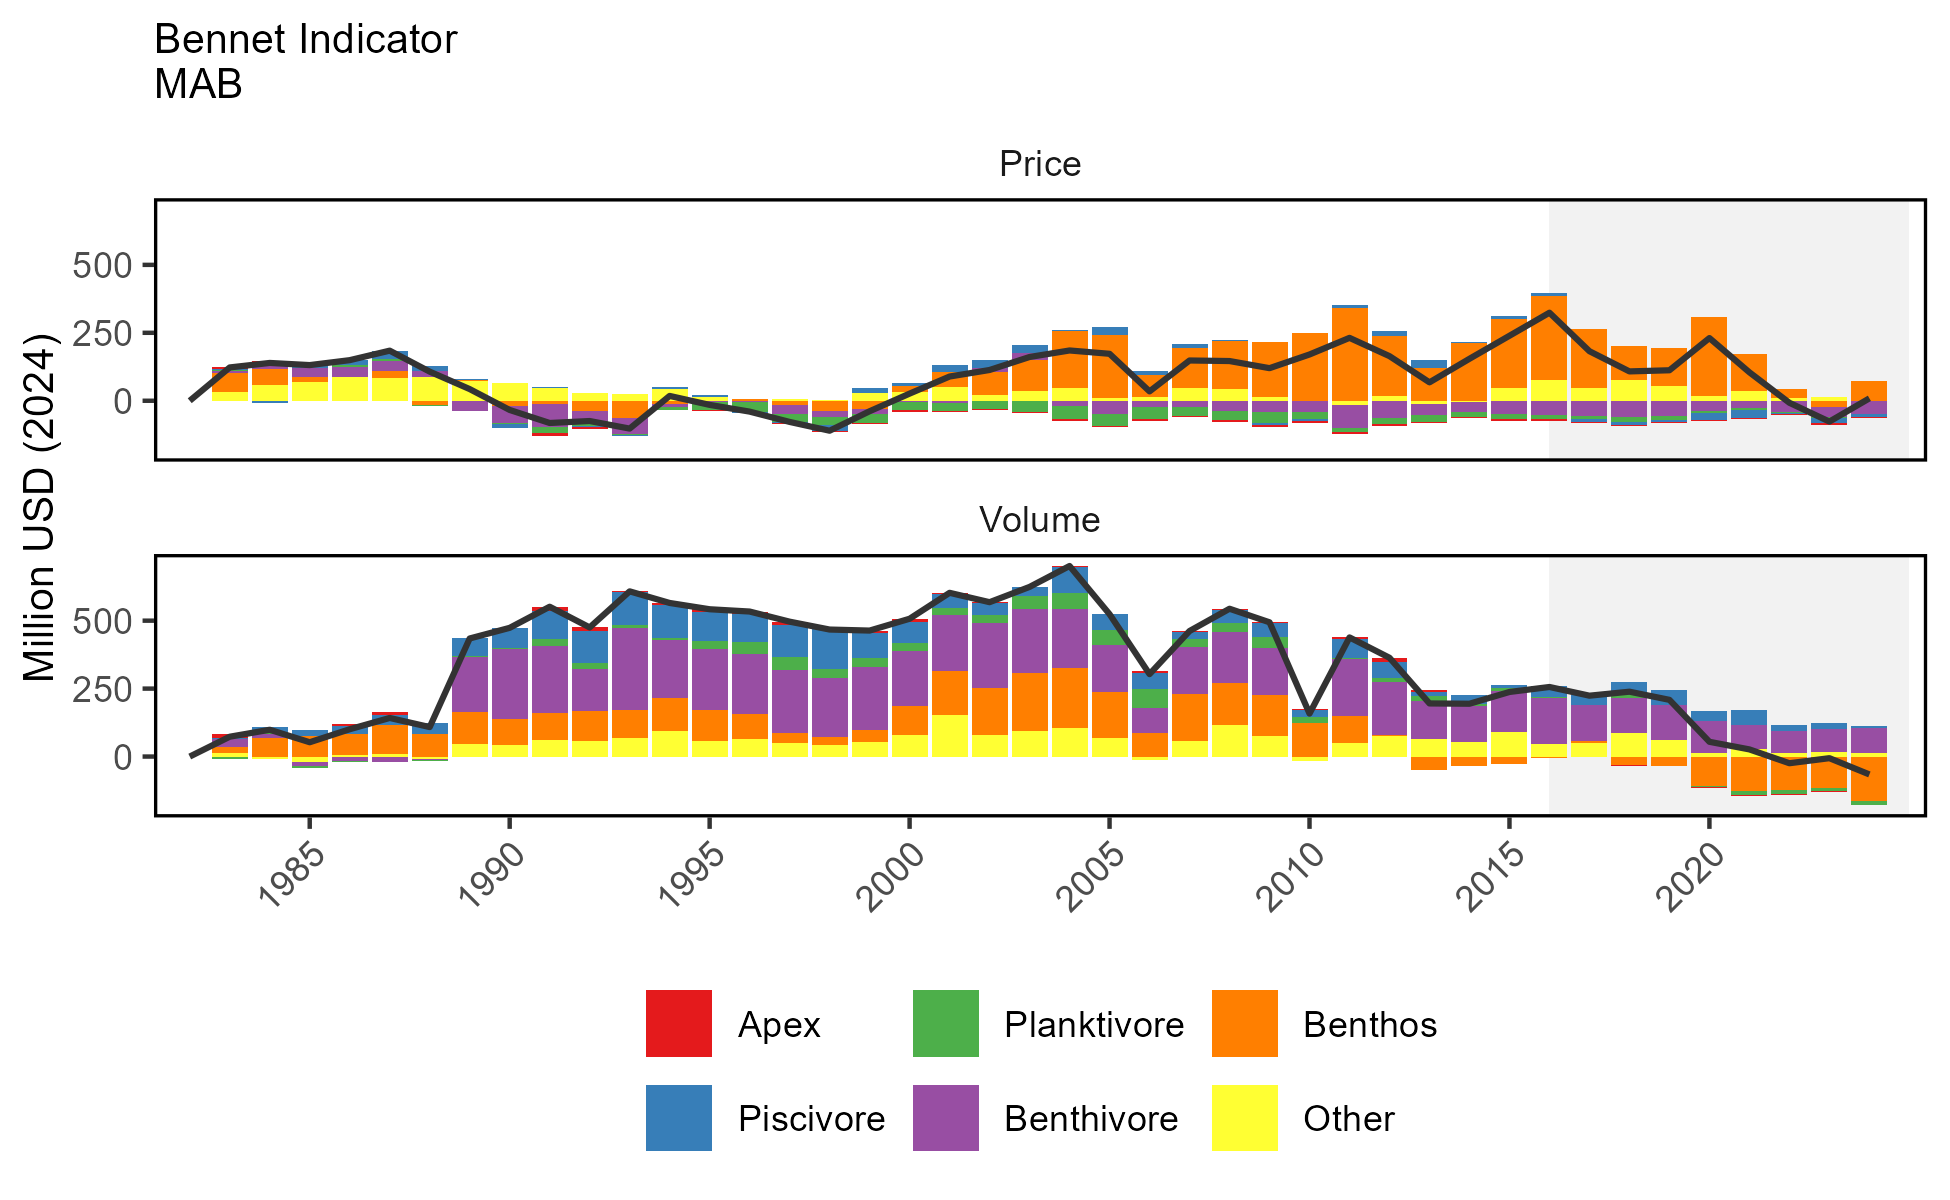
\includegraphics[width=1\linewidth,]{images/MidAtlantic/bennet_all_MidAtlantic_2026-03-27} 

}

\caption{Total price (top) and volume (bottom) indicators in 2024 dollars (black) for commercial landings, and individual guild contributions to each indicator, in the Mid-Atlantic Bight.}\label{fig:bennet-all}
\end{figure}

\begin{figure}[T]

{\centering 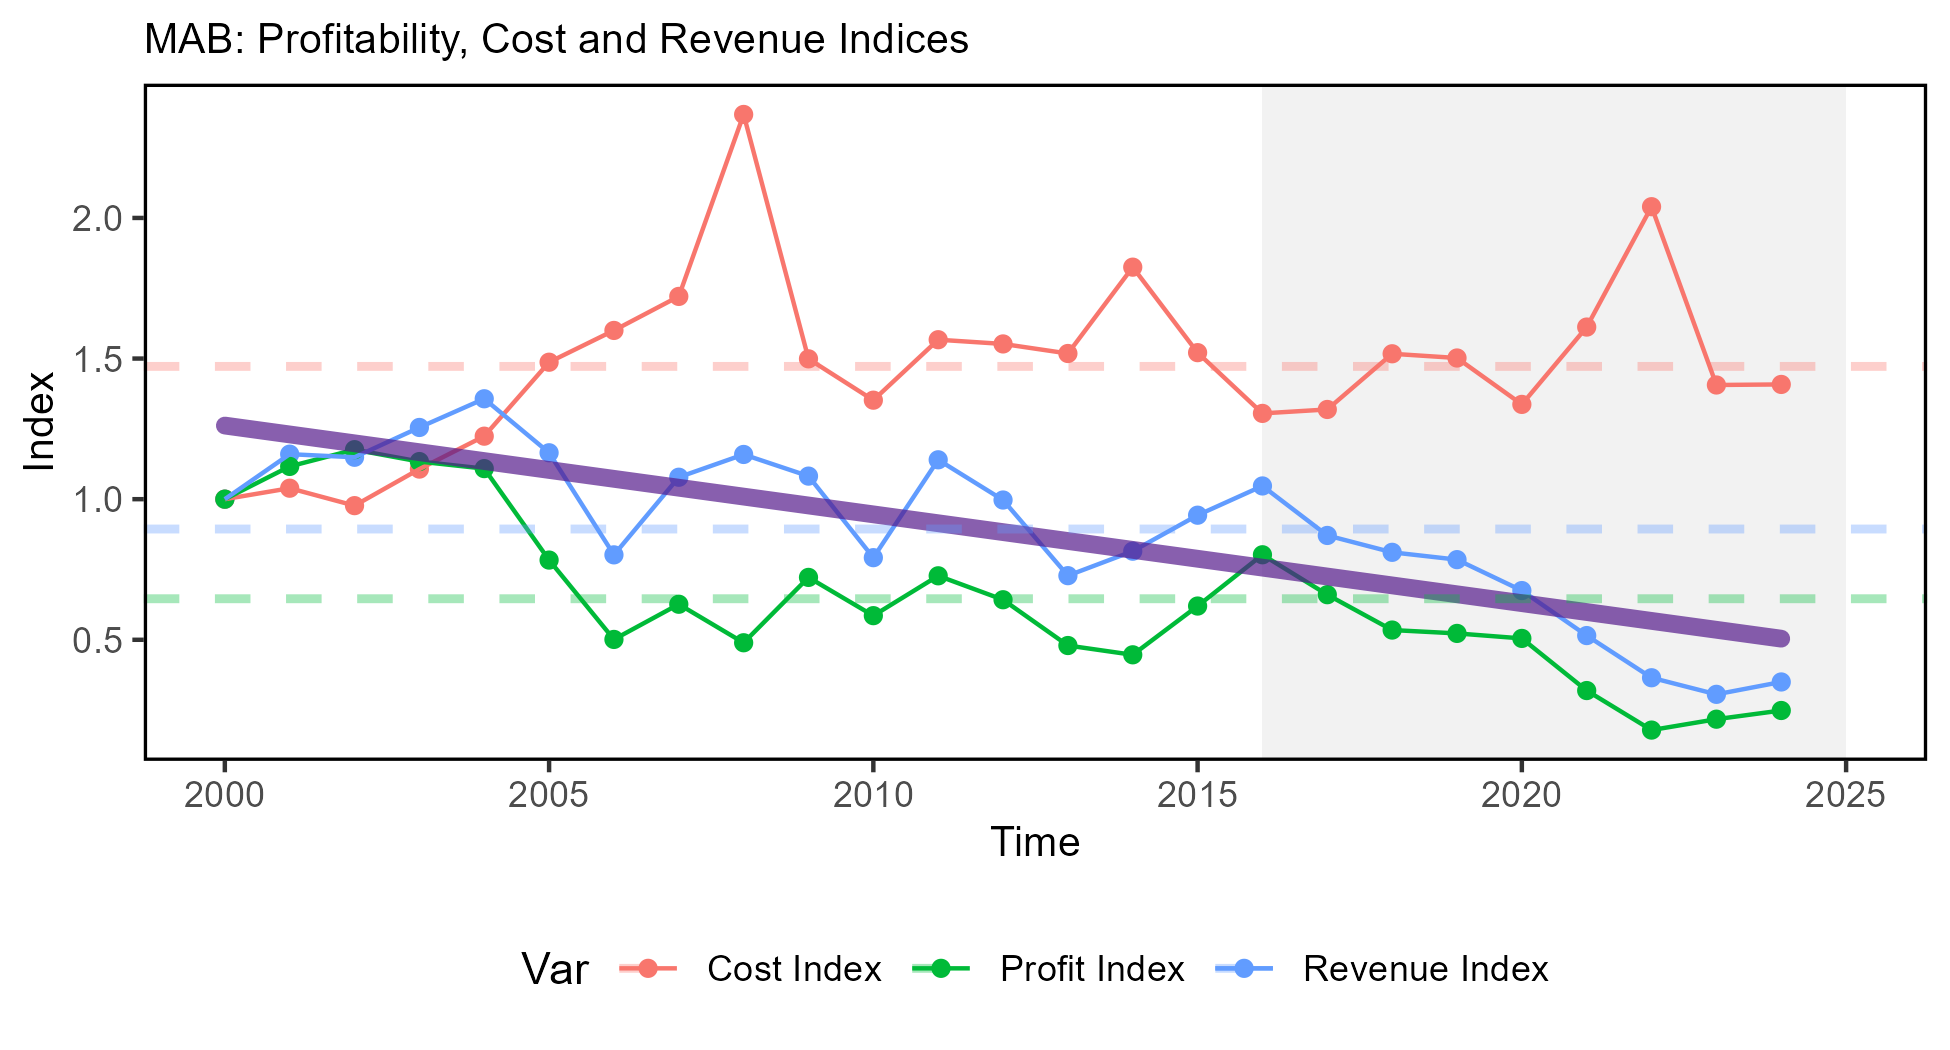
\includegraphics[width=1\linewidth,]{images/MidAtlantic/comdat_profit_MidAtlantic_2026-03-26} 

}

\caption{Profitability indices for Mid-Atlantic federally managed species: cost index (red), profit index (green), and revenue index (blue). Dashed lines represent the long-term annual means for each index. Long-term declining trend (purple) associated with revenue index.}\label{fig:comdat-profit}
\end{figure}

This year, we present new indicators of \href{https://noaa-edab.github.io/catalog/comdat_profit.html}{profitability}: indices of cost, revenue, and profit based on trips catching federally-managed species. In this index, costs pertain to trip costs, excluding labor, estimated for all federal trips in the region. The profit indicator is net-revenue, determined as the difference between trip revenue and trip costs. Trips were spatially allocated to compile regional indices. Indices are presented as values relative to 2000, the first year in the dataset. In the Mid-Atlantic, costs have fluctuated, but overall remain near the time series mean, despite some high costs in 2022, 2014 and 2008. The revenue index, however, has declined steadily since 2019 and is driving an overall decline in profits (Fig. \ref{fig:comdat-profit}).

For Mid-Atlantic ports, \href{https://noaa-edab.github.io/catalog/community_climate_vulnerability.html}{total vulnerability} of revenue is high for the entire time series \hyperref[social-and-community-risks]{(2000-2024)}, with no long-term trend. This suggests that Mid-Atlantic port commercial fishing revenue is highly reliant on climate-sensitive species for the entire time period assessed (Fig. \ref{fig:climatevul-rev}).

\begin{figure}[T]

{\centering 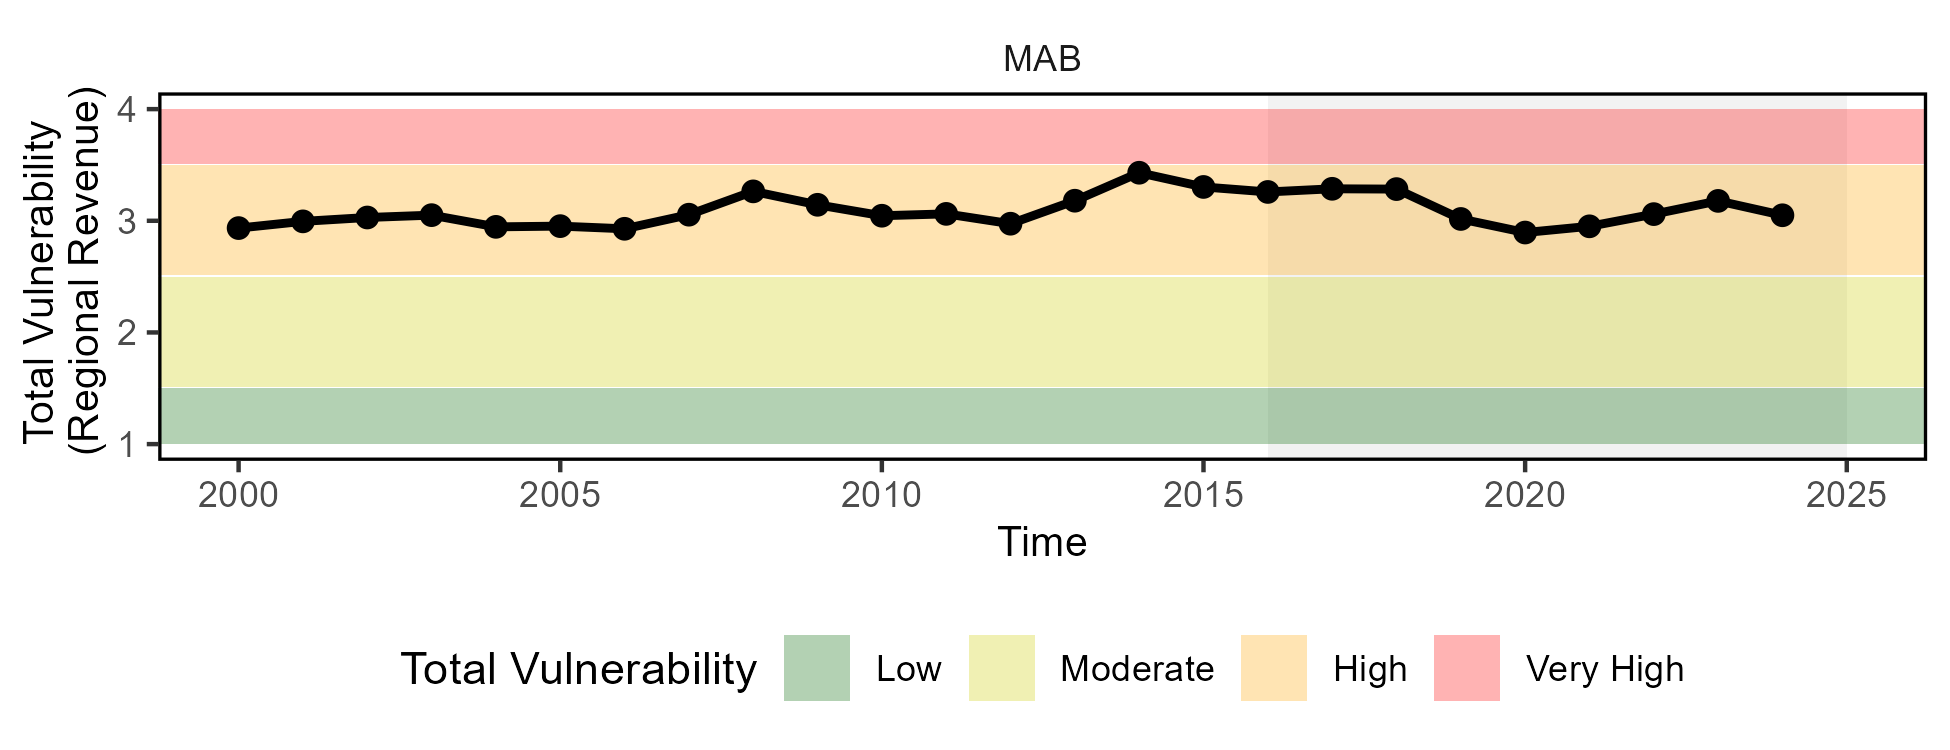
\includegraphics[width=1\linewidth,]{images/MidAtlantic/climatevul_rev_MidAtlantic_2026-03-26} 

}

\caption{Mid-Atlantic region total vulnerability of commercial revenue (sum of Mid-Atlantic port revenue weighted  by species vulnerability scores). Horizontal colored bars show different environmental variability risk levels. }\label{fig:climatevul-rev}
\end{figure}

\subsubsection{Implications}\label{implications-1}

Although the Mid-Atlantic region shows declining revenue since 2016 (Fig. \ref{fig:comm-revenue}), inflation-adjusted revenue from harvested species was still greater than 1982 levels until the past two years (Fig. \ref{fig:bennet}). However, revenue from MAFMC-managed species has been below 2000 levels in several of the past 24 years (Fig. \ref{fig:comdat-profit}). The Bennet Index demonstrates that this decline is driven by lower landing volumes, which were not offset by price increases. Declines in landings of surfclams and ocean quahogs since 2012 may reflect changes in surfclam and quahog aggregation or distribution patterns and/or changes to \href{https://noaa-edab.github.io/catalog/effective_sweptarea.html}{landings per unit effort}. Changes in other indicators, particularly those driving landings and those related to climate change, require monitoring as they may become important drivers of revenue in the future. Multiple stressors including \href{https://noaa-edab.github.io/catalog/bottom_temp_insitu.html}{warming} and \href{https://noaa-edab.github.io/catalog/ocean_acidification}{ocean acidification} are interacting in Mid-Atlantic shellfish habitats, particularly for surfclams, ocean quahogs, and scallops. This is reflected by the high environmental risk for landings from Mid-Atlantic ports.

\subsection{Recreational Opportunities}\label{recreational-opportunities}

\subsubsection{Indicators: Angler trips, fleet diversity}\label{indicators-angler-trips-fleet-diversity}

\href{https://noaa-edab.github.io/catalog/recdat.html}{Recreational effort} (angler trips) in the MAB increased from 1982 to 2010, but has since declined to near the long-term average (Fig. \ref{fig:rec-op}). However, there is a long-term declining trend in recreational fleet diversity (i.e., effort by shoreside, private boat, and for-hire anglers) (Fig. \ref{fig:rec-div}). Billfish landings were notably high in 2025 (See \href{https://noaa-edab.github.io/catalog/observation_synthesis_2025.html}{2025 Highlights} Section), and indicator time series are in development.

\begin{figure}[T]

{\centering 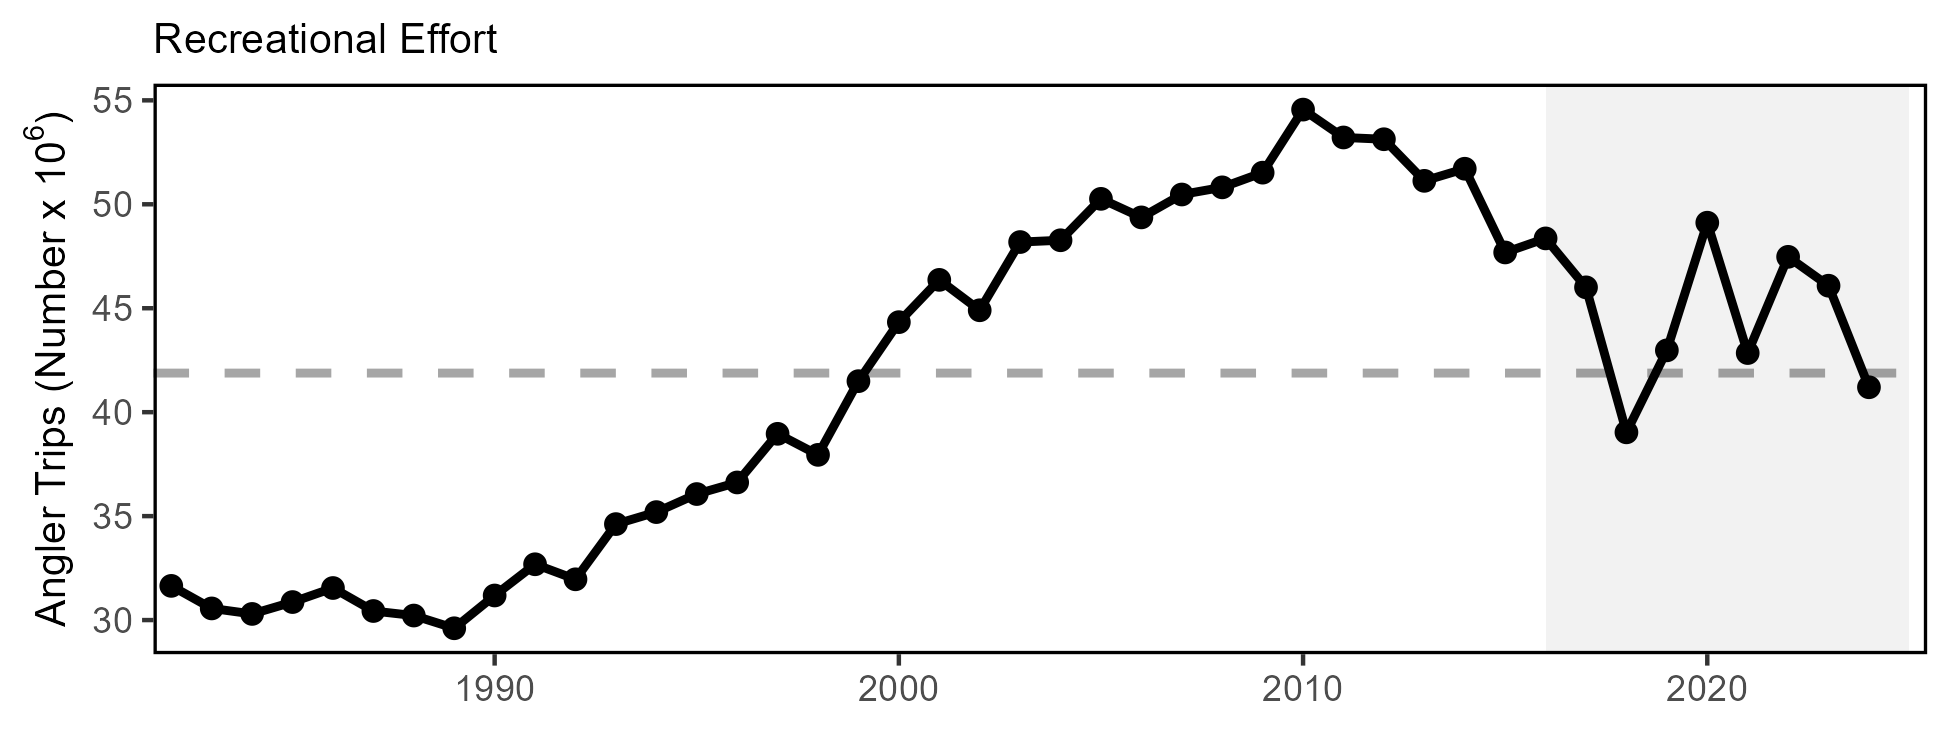
\includegraphics[width=1\linewidth,]{images/MidAtlantic/rec_op_MidAtlantic_2026-03-26} 

}

\caption{Recreational effort (total number of recreational angler trips from 1980-2024) in the Mid-Atlantic. Derived from NOAA Fisheries Marine Recreational Information Program Effort Time Series Query.}\label{fig:rec-op}
\end{figure}

\begin{figure}[T]

{\centering 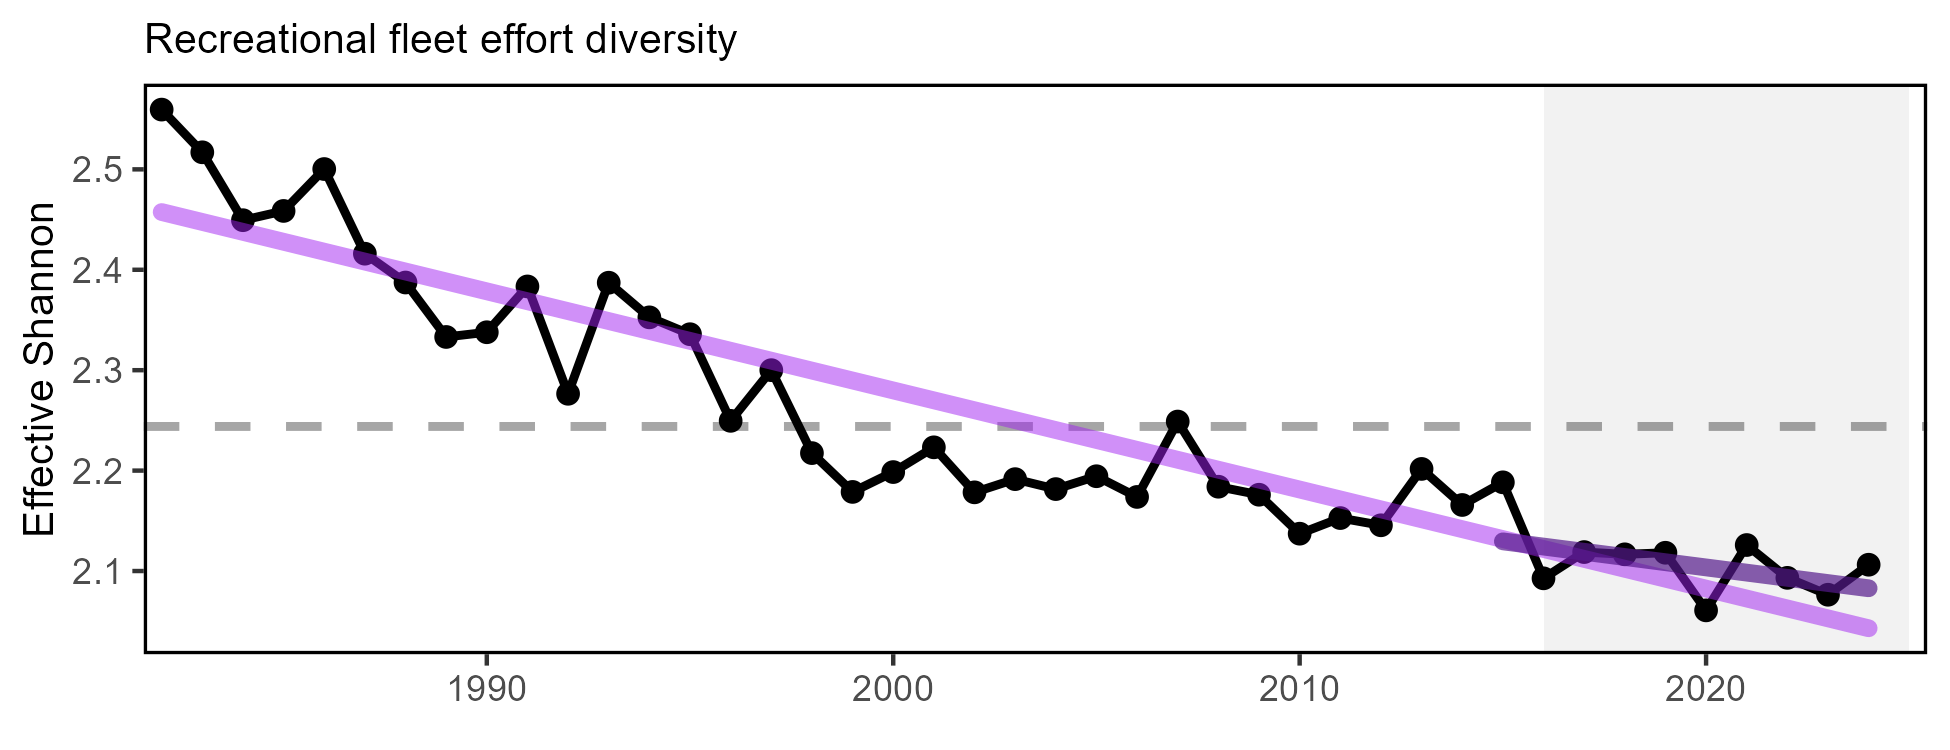
\includegraphics[width=1\linewidth,]{images/MidAtlantic/rec_div_MidAtlantic_2026-03-26} 

}

\caption{Recreational fleet effort diversity from 1980-2024 in the Mid-Atlantic, with significant decrease in long-term (light purple) and short-term (dark purple) trends.}\label{fig:rec-div}
\end{figure}

\subsubsection{Implications}\label{implications-2}

While the overall number of recreational trips in the MAB is above the long-term average, the continuing decline in recreational fleet effort diversity suggests, at least in part, changes in angler behavior. Future study is required to determine whether and to what extent the range and availability of recreational fishing options may drive these changes as well.

A contraction of party/charter trips (dropping from 2.2\% of trips in 2021 to 1.3\% in 2023) is the primary driver of the downward effort diversity trend, alongside a shift toward shorebased angling, which now makes up 60\% of trips. Private boat effort has remained consistent to 2022 values.

Managers should consider the differing species and fish sizes for shore-based and vessel-based anglers. Some species use inshore regions as nursery grounds while other species only come inshore as adults. Many states have developed shore-based regulations where the minimum size is lower than in other areas and sectors to maintain opportunities in the shore angling sector. The MAFMC is currently considering recreational sector separation which might establish different options for managing the for-hire sector from other modes.

\subsection{Social and Community Risks}\label{social-and-community-risks}

Fisheries management seeks to provide for sustained participation of fishing communities and to avoid adverse economic impacts to fishing communities. A new \href{https://noaa-edab.github.io/catalog/engagement.html?q=engage\#introduction-to-indicator-72}{composite indicator} (Port Commercial Fishing Activity Indicator or PCFA) utilizes NOAA data on dealers, fish landings, and commercial permits to explore trends in commercial fishing activity over time in top ports. This information can be used to understand how changes in fish stocks, regulations, and other social-ecological factors may have disparately impacted ports throughout the Greater Atlantic region.

The recreational engagement index has not been updated from last year and will be updated with similar methods as PCFA in future reports. The recreational \href{https://noaa-edab.github.io/catalog/engagement.html}{engagement} index demonstrates participation levels in recreational fishing in a given community relative to other coastal communities in a region.

The Community Social Vulnerability Indicators (CSVI) utilize U.S. Census American Community Survey data to describe social characteristics at the municipality level (i.e., not just the fishing community) and provide context for the municipalities utilized by commercial fishing industry participants. Fishing industry participants that live in and/or utilize resources in municipalities with relatively concerning socio-demographic conditions may be more vulnerable to changes. The personal disruption index addresses factors that reduce adaptability to change such as unemployment and educational level. The poverty index is a composite index that indicates a community's financial standing relative to other communities. The population composition index characterizes groups within communities that may be more vulnerable to change. CSVI information for communities highlighted in the PCFA and recreational engagement index have been updated with the most recent census data from 2023.

Coastal fishing communities worldwide have or are likely to experience social, economic, and cultural impacts from climate change, both negative (e.g., loss of infrastructure, fish stock decline) and positive (e.g., increased abundance of valuable species). Changes in marine fisheries as a consequence of climate change will require adaptation by coastal fishing communities and fisheries managers alike. The Community Environmental Variability Risk Indicators (CEVRI) were developed to help examine trends in risk related to dependence on species vulnerable to climate and environmental changes.

\subsubsection{Indicators: Port Commercial Fishing Activity and Community Social Vulnerability}\label{indicators-port-commercial-fishing-activity-and-community-social-vulnerability}

The \href{https://noaa-edab.github.io/catalog/engagement.html?q=engage\#introduction-to-indicator-72}{Port Commercial Fishing Activity Indicator (PCFA)} (Fig. \ref{fig:commercial-engagement}) highlights significant shifts in industry engagement across major regional ports. Newport News, VA, Ocean City, MD, Bronx, NY, and Point Pleasant Beach, Cape May, and Barnegat Light, NJ have lower fishing activity compared to their 2007--2011 averages. Because Bronx, NY and Newport News, VA also rank medium-high for socio-demographic vulnerability, industry participants in these municipalities face a higher risk from these changing conditions. The other four top communities show higher port activity since 2007-2011; most notably Hampton Bays/Shinnecock, NY showed an increase of 84\%. Currently North Carolina communities are not presented due to data limitations.

\begin{figure}[T]

{\centering 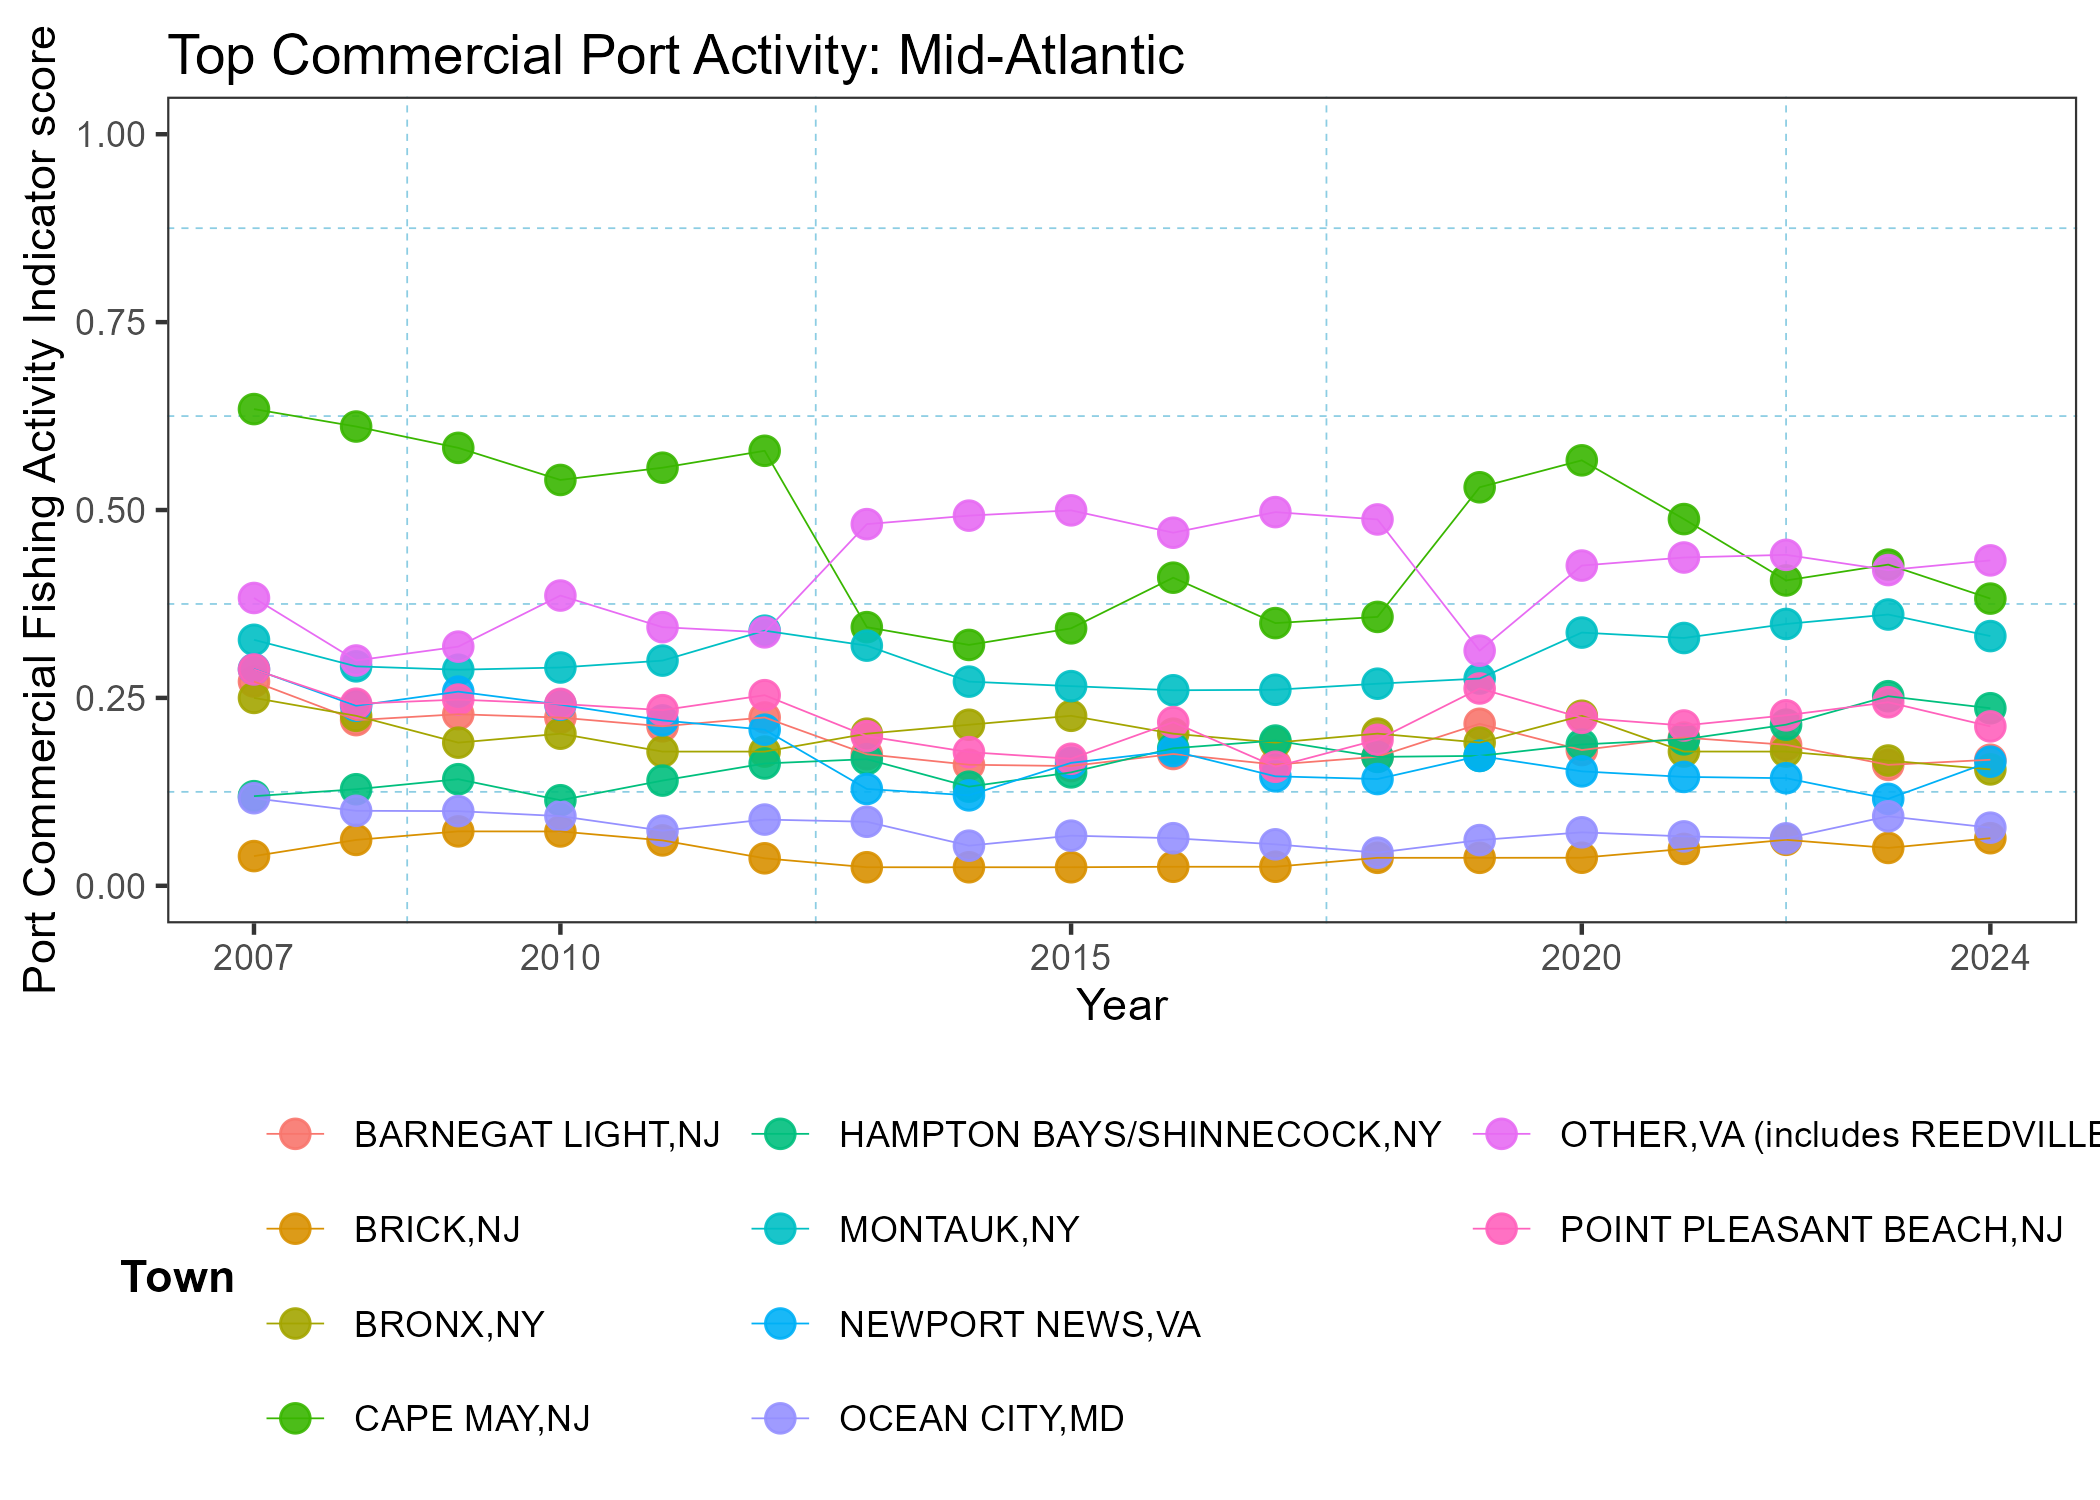
\includegraphics[width=1\linewidth,]{images/MidAtlantic/commercial_engagement_MidAtlantic_2026-03-26} 

}

\caption{Port Commercial Fishing Activity Indicator scores over time in the top 10 commercially active fishing ports in the Mid-Atlantic.}\label{fig:commercial-engagement}
\end{figure}

\global\setlength{\Oldarrayrulewidth}{\arrayrulewidth}

\global\setlength{\Oldtabcolsep}{\tabcolsep}

\setlength{\tabcolsep}{2pt}

\renewcommand*{\arraystretch}{1.5}



\providecommand{\ascline}[3]{\noalign{\global\arrayrulewidth #1}\arrayrulecolor[HTML]{#2}\cline{#3}}

\begin{longtable}[c]{|p{2.03in}|p{1.38in}|p{1.61in}|p{0.71in}}

\caption{Community\ Vulnerability\ factor\ rankings\ for\ the\ municipalities\ housing\ the\ top\ 10\ commercially\ active\ Mid-Atlantic\ ports}\label{tab:comvultab}\\

\ascline{1.5pt}{666666}{1-4}

\multicolumn{1}{>{\raggedright}m{\dimexpr 2.03in+0\tabcolsep}}{\textcolor[HTML]{000000}{\fontsize{9}{9}\selectfont{Community}}} & \multicolumn{1}{>{\raggedright}m{\dimexpr 1.38in+0\tabcolsep}}{\textcolor[HTML]{000000}{\fontsize{9}{9}\selectfont{Personal\ Disruption}}} & \multicolumn{1}{>{\raggedright}m{\dimexpr 1.61in+0\tabcolsep}}{\textcolor[HTML]{000000}{\fontsize{9}{9}\selectfont{Population\ Composition}}} & \multicolumn{1}{>{\raggedright}m{\dimexpr 0.71in+0\tabcolsep}}{\textcolor[HTML]{000000}{\fontsize{9}{9}\selectfont{Poverty}}} \\

\ascline{1.5pt}{666666}{1-4}\endfirsthead \caption[]{Community\ Vulnerability\ factor\ rankings\ for\ the\ municipalities\ housing\ the\ top\ 10\ commercially\ active\ Mid-Atlantic\ ports}\label{tab:comvultab}\\

\ascline{1.5pt}{666666}{1-4}

\multicolumn{1}{>{\raggedright}m{\dimexpr 2.03in+0\tabcolsep}}{\textcolor[HTML]{000000}{\fontsize{9}{9}\selectfont{Community}}} & \multicolumn{1}{>{\raggedright}m{\dimexpr 1.38in+0\tabcolsep}}{\textcolor[HTML]{000000}{\fontsize{9}{9}\selectfont{Personal\ Disruption}}} & \multicolumn{1}{>{\raggedright}m{\dimexpr 1.61in+0\tabcolsep}}{\textcolor[HTML]{000000}{\fontsize{9}{9}\selectfont{Population\ Composition}}} & \multicolumn{1}{>{\raggedright}m{\dimexpr 0.71in+0\tabcolsep}}{\textcolor[HTML]{000000}{\fontsize{9}{9}\selectfont{Poverty}}} \\

\ascline{1.5pt}{666666}{1-4}\endhead



\multicolumn{1}{>{\raggedright}m{\dimexpr 2.03in+0\tabcolsep}}{\textcolor[HTML]{000000}{\fontsize{9}{9}\selectfont{Bronx,\ NY}}} & \multicolumn{1}{>{\raggedright}m{\dimexpr 1.38in+0\tabcolsep}}{\textcolor[HTML]{000000}{\fontsize{9}{9}\selectfont{high}}} & \multicolumn{1}{>{\raggedright}m{\dimexpr 1.61in+0\tabcolsep}}{\textcolor[HTML]{000000}{\fontsize{9}{9}\selectfont{high}}} & \multicolumn{1}{>{\raggedright}m{\dimexpr 0.71in+0\tabcolsep}}{\textcolor[HTML]{000000}{\fontsize{9}{9}\selectfont{high}}} \\





\multicolumn{1}{>{\raggedright}m{\dimexpr 2.03in+0\tabcolsep}}{\textcolor[HTML]{000000}{\fontsize{9}{9}\selectfont{Newport\ News,\ VA}}} & \multicolumn{1}{>{\raggedright}m{\dimexpr 1.38in+0\tabcolsep}}{\textcolor[HTML]{000000}{\fontsize{9}{9}\selectfont{med}}} & \multicolumn{1}{>{\raggedright}m{\dimexpr 1.61in+0\tabcolsep}}{\textcolor[HTML]{000000}{\fontsize{9}{9}\selectfont{med\ high}}} & \multicolumn{1}{>{\raggedright}m{\dimexpr 0.71in+0\tabcolsep}}{\textcolor[HTML]{000000}{\fontsize{9}{9}\selectfont{med}}} \\





\multicolumn{1}{>{\raggedright}m{\dimexpr 2.03in+0\tabcolsep}}{\textcolor[HTML]{000000}{\fontsize{9}{9}\selectfont{Hampton\ Bays/Shinnecock,\ NY}}} & \multicolumn{1}{>{\raggedright}m{\dimexpr 1.38in+0\tabcolsep}}{\textcolor[HTML]{000000}{\fontsize{9}{9}\selectfont{low}}} & \multicolumn{1}{>{\raggedright}m{\dimexpr 1.61in+0\tabcolsep}}{\textcolor[HTML]{000000}{\fontsize{9}{9}\selectfont{med\ high}}} & \multicolumn{1}{>{\raggedright}m{\dimexpr 0.71in+0\tabcolsep}}{\textcolor[HTML]{000000}{\fontsize{9}{9}\selectfont{low}}} \\





\multicolumn{1}{>{\raggedright}m{\dimexpr 2.03in+0\tabcolsep}}{\textcolor[HTML]{000000}{\fontsize{9}{9}\selectfont{Ocean\ City,\ MD}}} & \multicolumn{1}{>{\raggedright}m{\dimexpr 1.38in+0\tabcolsep}}{\textcolor[HTML]{000000}{\fontsize{9}{9}\selectfont{med}}} & \multicolumn{1}{>{\raggedright}m{\dimexpr 1.61in+0\tabcolsep}}{\textcolor[HTML]{000000}{\fontsize{9}{9}\selectfont{low}}} & \multicolumn{1}{>{\raggedright}m{\dimexpr 0.71in+0\tabcolsep}}{\textcolor[HTML]{000000}{\fontsize{9}{9}\selectfont{low}}} \\





\multicolumn{1}{>{\raggedright}m{\dimexpr 2.03in+0\tabcolsep}}{\textcolor[HTML]{000000}{\fontsize{9}{9}\selectfont{Barnegat\ Light,\ NJ}}} & \multicolumn{1}{>{\raggedright}m{\dimexpr 1.38in+0\tabcolsep}}{\textcolor[HTML]{000000}{\fontsize{9}{9}\selectfont{low}}} & \multicolumn{1}{>{\raggedright}m{\dimexpr 1.61in+0\tabcolsep}}{\textcolor[HTML]{000000}{\fontsize{9}{9}\selectfont{low}}} & \multicolumn{1}{>{\raggedright}m{\dimexpr 0.71in+0\tabcolsep}}{\textcolor[HTML]{000000}{\fontsize{9}{9}\selectfont{low}}} \\





\multicolumn{1}{>{\raggedright}m{\dimexpr 2.03in+0\tabcolsep}}{\textcolor[HTML]{000000}{\fontsize{9}{9}\selectfont{Cape\ May,\ NJ}}} & \multicolumn{1}{>{\raggedright}m{\dimexpr 1.38in+0\tabcolsep}}{\textcolor[HTML]{000000}{\fontsize{9}{9}\selectfont{low}}} & \multicolumn{1}{>{\raggedright}m{\dimexpr 1.61in+0\tabcolsep}}{\textcolor[HTML]{000000}{\fontsize{9}{9}\selectfont{low}}} & \multicolumn{1}{>{\raggedright}m{\dimexpr 0.71in+0\tabcolsep}}{\textcolor[HTML]{000000}{\fontsize{9}{9}\selectfont{low}}} \\





\multicolumn{1}{>{\raggedright}m{\dimexpr 2.03in+0\tabcolsep}}{\textcolor[HTML]{000000}{\fontsize{9}{9}\selectfont{Point\ Pleasant\ Beach,\ NJ}}} & \multicolumn{1}{>{\raggedright}m{\dimexpr 1.38in+0\tabcolsep}}{\textcolor[HTML]{000000}{\fontsize{9}{9}\selectfont{low}}} & \multicolumn{1}{>{\raggedright}m{\dimexpr 1.61in+0\tabcolsep}}{\textcolor[HTML]{000000}{\fontsize{9}{9}\selectfont{low}}} & \multicolumn{1}{>{\raggedright}m{\dimexpr 0.71in+0\tabcolsep}}{\textcolor[HTML]{000000}{\fontsize{9}{9}\selectfont{low}}} \\





\multicolumn{1}{>{\raggedright}m{\dimexpr 2.03in+0\tabcolsep}}{\textcolor[HTML]{000000}{\fontsize{9}{9}\selectfont{Brick,\ NJ}}} & \multicolumn{1}{>{\raggedright}m{\dimexpr 1.38in+0\tabcolsep}}{\textcolor[HTML]{000000}{\fontsize{9}{9}\selectfont{low}}} & \multicolumn{1}{>{\raggedright}m{\dimexpr 1.61in+0\tabcolsep}}{\textcolor[HTML]{000000}{\fontsize{9}{9}\selectfont{low}}} & \multicolumn{1}{>{\raggedright}m{\dimexpr 0.71in+0\tabcolsep}}{\textcolor[HTML]{000000}{\fontsize{9}{9}\selectfont{low}}} \\





\multicolumn{1}{>{\raggedright}m{\dimexpr 2.03in+0\tabcolsep}}{\textcolor[HTML]{000000}{\fontsize{9}{9}\selectfont{Montauk,\ NY}}} & \multicolumn{1}{>{\raggedright}m{\dimexpr 1.38in+0\tabcolsep}}{\textcolor[HTML]{000000}{\fontsize{9}{9}\selectfont{low}}} & \multicolumn{1}{>{\raggedright}m{\dimexpr 1.61in+0\tabcolsep}}{\textcolor[HTML]{000000}{\fontsize{9}{9}\selectfont{low}}} & \multicolumn{1}{>{\raggedright}m{\dimexpr 0.71in+0\tabcolsep}}{\textcolor[HTML]{000000}{\fontsize{9}{9}\selectfont{low}}} \\





\multicolumn{1}{>{\raggedright}m{\dimexpr 2.03in+0\tabcolsep}}{\textcolor[HTML]{000000}{\fontsize{9}{9}\selectfont{Reedville,\ VA}}} & \multicolumn{1}{>{\raggedright}m{\dimexpr 1.38in+0\tabcolsep}}{\textcolor[HTML]{000000}{\fontsize{9}{9}\selectfont{low}}} & \multicolumn{1}{>{\raggedright}m{\dimexpr 1.61in+0\tabcolsep}}{\textcolor[HTML]{000000}{\fontsize{9}{9}\selectfont{low}}} & \multicolumn{1}{>{\raggedright}m{\dimexpr 0.71in+0\tabcolsep}}{\textcolor[HTML]{000000}{\fontsize{9}{9}\selectfont{low}}} \\

\ascline{1.5pt}{666666}{1-4}



\end{longtable}



\arrayrulecolor[HTML]{000000}

\global\setlength{\arrayrulewidth}{\Oldarrayrulewidth}

\global\setlength{\tabcolsep}{\Oldtabcolsep}

\renewcommand*{\arraystretch}{1}

Of those included in the top-ranked recreational communities, both Morehead City, NC and Virginia Beach, VA had medium or higher ranks for at least one socio-demographic indicator (Table \ref{tab:recvultab}) (Fig. \ref{recreational-engagement}). This suggests that future changes to recreational fishing conditions may disproportionately impact these places.

\begin{figure}[T]

{\centering 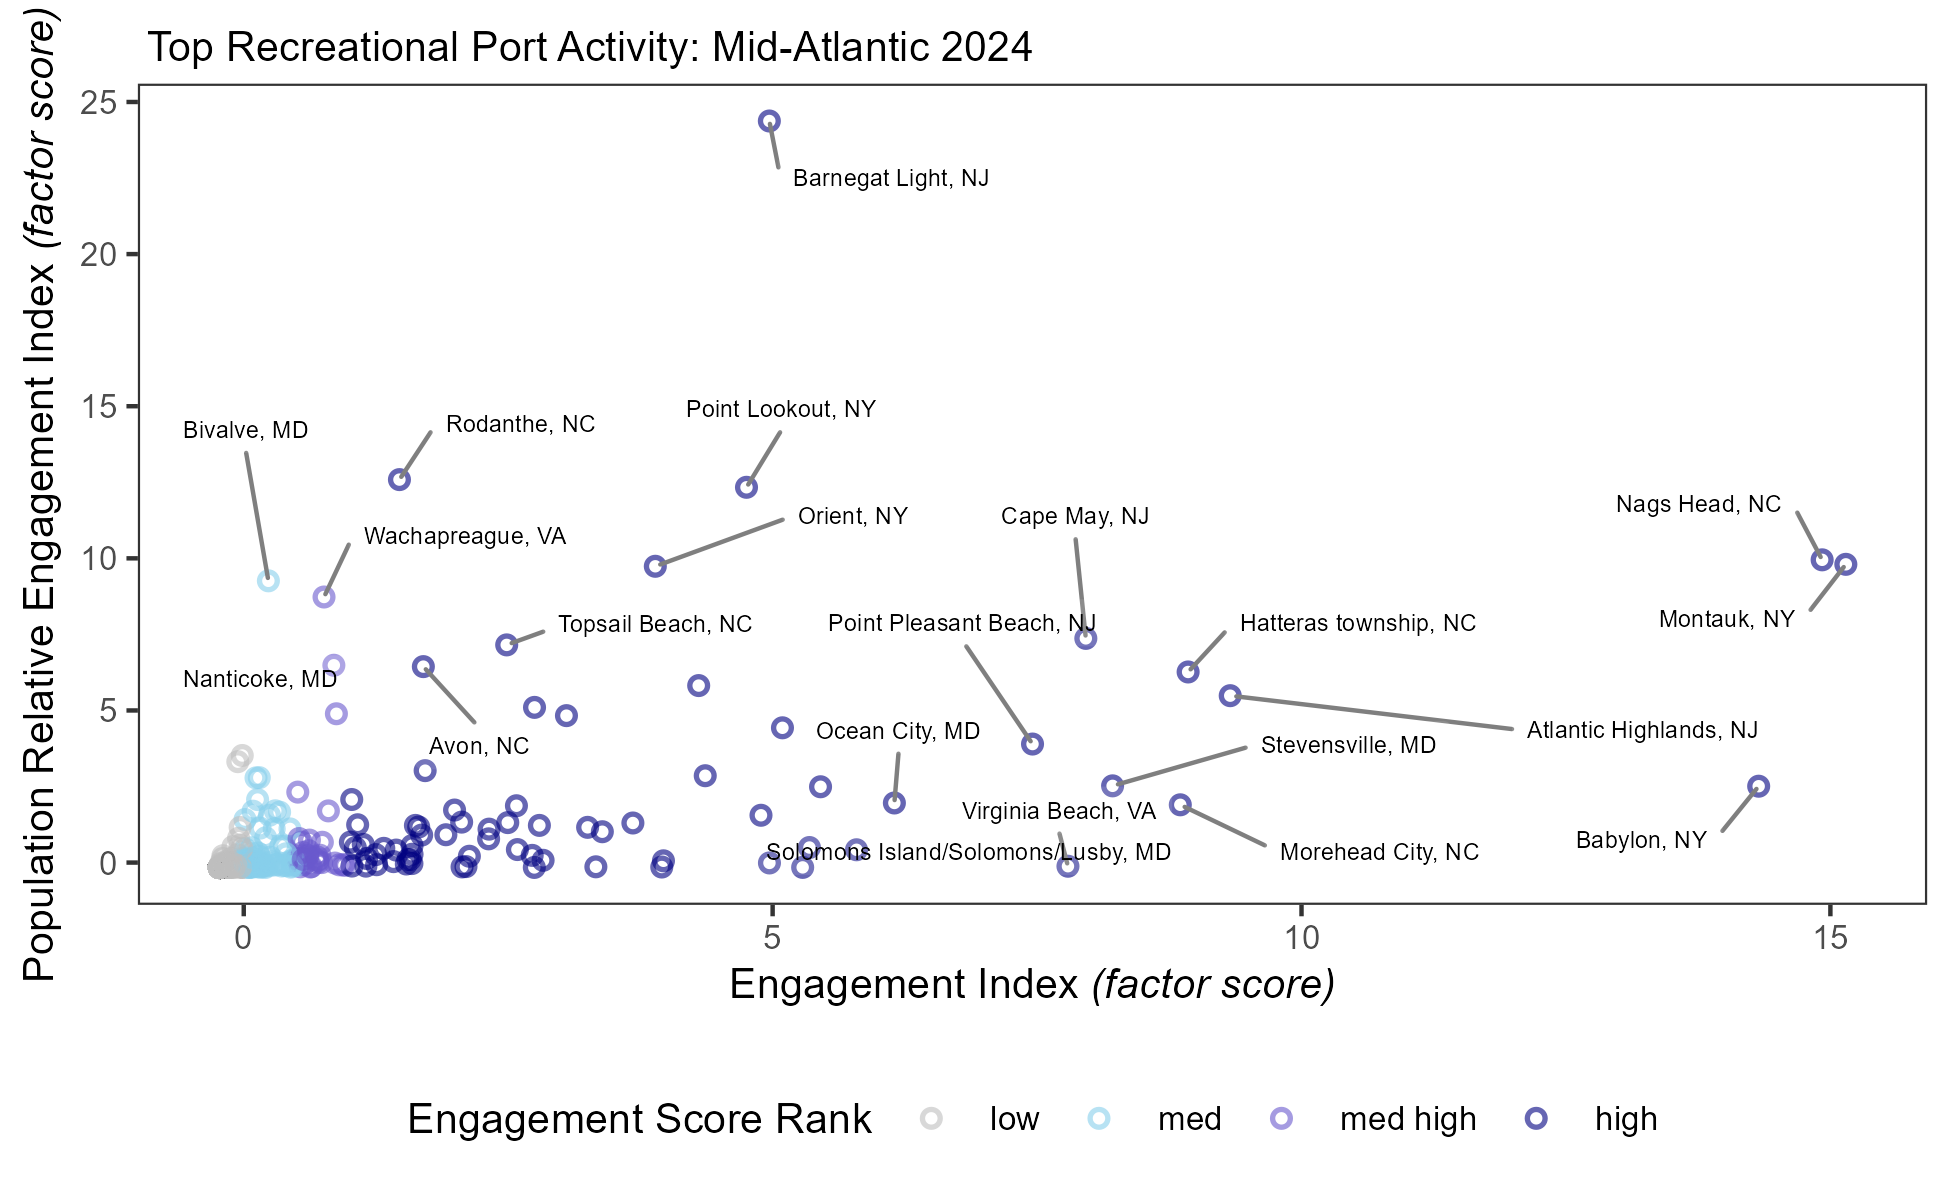
\includegraphics[width=1\linewidth,]{images/MidAtlantic/recreational_engagement_MidAtlantic_2026-03-26} 

}

\caption{Recreational engagement and population relative engagement with labels for the top recreationally engaged fishing communities in the Mid-Atlantic (last updated 2024).}\label{fig:recreational-engagement}
\end{figure}

\global\setlength{\Oldarrayrulewidth}{\arrayrulewidth}

\global\setlength{\Oldtabcolsep}{\tabcolsep}

\setlength{\tabcolsep}{2pt}

\renewcommand*{\arraystretch}{1.5}



\providecommand{\ascline}[3]{\noalign{\global\arrayrulewidth #1}\arrayrulecolor[HTML]{#2}\cline{#3}}

\begin{longtable}[c]{|p{1.70in}|p{1.38in}|p{1.61in}|p{0.80in}}

\caption{Community\ Vulnerability\ factor\ rankings\ for\ the\ top\ 10\ recreationally\ engaged\ Mid-Atlantic\ Ports}\label{tab:recvultab}\\

\ascline{1.5pt}{666666}{1-4}

\multicolumn{1}{>{\raggedright}m{\dimexpr 1.7in+0\tabcolsep}}{\textcolor[HTML]{000000}{\fontsize{9}{9}\selectfont{Community}}} & \multicolumn{1}{>{\raggedright}m{\dimexpr 1.38in+0\tabcolsep}}{\textcolor[HTML]{000000}{\fontsize{9}{9}\selectfont{Personal\ Disruption}}} & \multicolumn{1}{>{\raggedright}m{\dimexpr 1.61in+0\tabcolsep}}{\textcolor[HTML]{000000}{\fontsize{9}{9}\selectfont{Population\ Composition}}} & \multicolumn{1}{>{\raggedright}m{\dimexpr 0.8in+0\tabcolsep}}{\textcolor[HTML]{000000}{\fontsize{9}{9}\selectfont{Poverty}}} \\

\ascline{1.5pt}{666666}{1-4}\endfirsthead \caption[]{Community\ Vulnerability\ factor\ rankings\ for\ the\ top\ 10\ recreationally\ engaged\ Mid-Atlantic\ Ports}\label{tab:recvultab}\\

\ascline{1.5pt}{666666}{1-4}

\multicolumn{1}{>{\raggedright}m{\dimexpr 1.7in+0\tabcolsep}}{\textcolor[HTML]{000000}{\fontsize{9}{9}\selectfont{Community}}} & \multicolumn{1}{>{\raggedright}m{\dimexpr 1.38in+0\tabcolsep}}{\textcolor[HTML]{000000}{\fontsize{9}{9}\selectfont{Personal\ Disruption}}} & \multicolumn{1}{>{\raggedright}m{\dimexpr 1.61in+0\tabcolsep}}{\textcolor[HTML]{000000}{\fontsize{9}{9}\selectfont{Population\ Composition}}} & \multicolumn{1}{>{\raggedright}m{\dimexpr 0.8in+0\tabcolsep}}{\textcolor[HTML]{000000}{\fontsize{9}{9}\selectfont{Poverty}}} \\

\ascline{1.5pt}{666666}{1-4}\endhead



\multicolumn{1}{>{\raggedright}m{\dimexpr 1.7in+0\tabcolsep}}{\textcolor[HTML]{000000}{\fontsize{9}{9}\selectfont{Morehead\ City,\ NC}}} & \multicolumn{1}{>{\raggedright}m{\dimexpr 1.38in+0\tabcolsep}}{\textcolor[HTML]{000000}{\fontsize{9}{9}\selectfont{med}}} & \multicolumn{1}{>{\raggedright}m{\dimexpr 1.61in+0\tabcolsep}}{\textcolor[HTML]{000000}{\fontsize{9}{9}\selectfont{low}}} & \multicolumn{1}{>{\raggedright}m{\dimexpr 0.8in+0\tabcolsep}}{\textcolor[HTML]{000000}{\fontsize{9}{9}\selectfont{med\ high}}} \\





\multicolumn{1}{>{\raggedright}m{\dimexpr 1.7in+0\tabcolsep}}{\textcolor[HTML]{000000}{\fontsize{9}{9}\selectfont{Virginia\ Beach,\ VA}}} & \multicolumn{1}{>{\raggedright}m{\dimexpr 1.38in+0\tabcolsep}}{\textcolor[HTML]{000000}{\fontsize{9}{9}\selectfont{low}}} & \multicolumn{1}{>{\raggedright}m{\dimexpr 1.61in+0\tabcolsep}}{\textcolor[HTML]{000000}{\fontsize{9}{9}\selectfont{med}}} & \multicolumn{1}{>{\raggedright}m{\dimexpr 0.8in+0\tabcolsep}}{\textcolor[HTML]{000000}{\fontsize{9}{9}\selectfont{low}}} \\





\multicolumn{1}{>{\raggedright}m{\dimexpr 1.7in+0\tabcolsep}}{\textcolor[HTML]{000000}{\fontsize{9}{9}\selectfont{Stevensville,\ MD}}} & \multicolumn{1}{>{\raggedright}m{\dimexpr 1.38in+0\tabcolsep}}{\textcolor[HTML]{000000}{\fontsize{9}{9}\selectfont{low}}} & \multicolumn{1}{>{\raggedright}m{\dimexpr 1.61in+0\tabcolsep}}{\textcolor[HTML]{000000}{\fontsize{9}{9}\selectfont{low}}} & \multicolumn{1}{>{\raggedright}m{\dimexpr 0.8in+0\tabcolsep}}{\textcolor[HTML]{000000}{\fontsize{9}{9}\selectfont{low}}} \\





\multicolumn{1}{>{\raggedright}m{\dimexpr 1.7in+0\tabcolsep}}{\textcolor[HTML]{000000}{\fontsize{9}{9}\selectfont{Nags\ Head,\ NC}}} & \multicolumn{1}{>{\raggedright}m{\dimexpr 1.38in+0\tabcolsep}}{\textcolor[HTML]{000000}{\fontsize{9}{9}\selectfont{low}}} & \multicolumn{1}{>{\raggedright}m{\dimexpr 1.61in+0\tabcolsep}}{\textcolor[HTML]{000000}{\fontsize{9}{9}\selectfont{low}}} & \multicolumn{1}{>{\raggedright}m{\dimexpr 0.8in+0\tabcolsep}}{\textcolor[HTML]{000000}{\fontsize{9}{9}\selectfont{low}}} \\





\multicolumn{1}{>{\raggedright}m{\dimexpr 1.7in+0\tabcolsep}}{\textcolor[HTML]{000000}{\fontsize{9}{9}\selectfont{Hatteras\ Township,\ NC}}} & \multicolumn{1}{>{\raggedright}m{\dimexpr 1.38in+0\tabcolsep}}{\textcolor[HTML]{000000}{\fontsize{9}{9}\selectfont{low}}} & \multicolumn{1}{>{\raggedright}m{\dimexpr 1.61in+0\tabcolsep}}{\textcolor[HTML]{000000}{\fontsize{9}{9}\selectfont{low}}} & \multicolumn{1}{>{\raggedright}m{\dimexpr 0.8in+0\tabcolsep}}{\textcolor[HTML]{000000}{\fontsize{9}{9}\selectfont{low}}} \\





\multicolumn{1}{>{\raggedright}m{\dimexpr 1.7in+0\tabcolsep}}{\textcolor[HTML]{000000}{\fontsize{9}{9}\selectfont{Atlantic\ Highlands,\ NJ}}} & \multicolumn{1}{>{\raggedright}m{\dimexpr 1.38in+0\tabcolsep}}{\textcolor[HTML]{000000}{\fontsize{9}{9}\selectfont{low}}} & \multicolumn{1}{>{\raggedright}m{\dimexpr 1.61in+0\tabcolsep}}{\textcolor[HTML]{000000}{\fontsize{9}{9}\selectfont{low}}} & \multicolumn{1}{>{\raggedright}m{\dimexpr 0.8in+0\tabcolsep}}{\textcolor[HTML]{000000}{\fontsize{9}{9}\selectfont{low}}} \\





\multicolumn{1}{>{\raggedright}m{\dimexpr 1.7in+0\tabcolsep}}{\textcolor[HTML]{000000}{\fontsize{9}{9}\selectfont{Cape\ May,\ NJ}}} & \multicolumn{1}{>{\raggedright}m{\dimexpr 1.38in+0\tabcolsep}}{\textcolor[HTML]{000000}{\fontsize{9}{9}\selectfont{low}}} & \multicolumn{1}{>{\raggedright}m{\dimexpr 1.61in+0\tabcolsep}}{\textcolor[HTML]{000000}{\fontsize{9}{9}\selectfont{low}}} & \multicolumn{1}{>{\raggedright}m{\dimexpr 0.8in+0\tabcolsep}}{\textcolor[HTML]{000000}{\fontsize{9}{9}\selectfont{low}}} \\





\multicolumn{1}{>{\raggedright}m{\dimexpr 1.7in+0\tabcolsep}}{\textcolor[HTML]{000000}{\fontsize{9}{9}\selectfont{Point\ Pleasant\ Beach,\ NJ}}} & \multicolumn{1}{>{\raggedright}m{\dimexpr 1.38in+0\tabcolsep}}{\textcolor[HTML]{000000}{\fontsize{9}{9}\selectfont{low}}} & \multicolumn{1}{>{\raggedright}m{\dimexpr 1.61in+0\tabcolsep}}{\textcolor[HTML]{000000}{\fontsize{9}{9}\selectfont{low}}} & \multicolumn{1}{>{\raggedright}m{\dimexpr 0.8in+0\tabcolsep}}{\textcolor[HTML]{000000}{\fontsize{9}{9}\selectfont{low}}} \\





\multicolumn{1}{>{\raggedright}m{\dimexpr 1.7in+0\tabcolsep}}{\textcolor[HTML]{000000}{\fontsize{9}{9}\selectfont{Babylon,\ NY}}} & \multicolumn{1}{>{\raggedright}m{\dimexpr 1.38in+0\tabcolsep}}{\textcolor[HTML]{000000}{\fontsize{9}{9}\selectfont{low}}} & \multicolumn{1}{>{\raggedright}m{\dimexpr 1.61in+0\tabcolsep}}{\textcolor[HTML]{000000}{\fontsize{9}{9}\selectfont{low}}} & \multicolumn{1}{>{\raggedright}m{\dimexpr 0.8in+0\tabcolsep}}{\textcolor[HTML]{000000}{\fontsize{9}{9}\selectfont{low}}} \\





\multicolumn{1}{>{\raggedright}m{\dimexpr 1.7in+0\tabcolsep}}{\textcolor[HTML]{000000}{\fontsize{9}{9}\selectfont{Montauk,\ NY}}} & \multicolumn{1}{>{\raggedright}m{\dimexpr 1.38in+0\tabcolsep}}{\textcolor[HTML]{000000}{\fontsize{9}{9}\selectfont{low}}} & \multicolumn{1}{>{\raggedright}m{\dimexpr 1.61in+0\tabcolsep}}{\textcolor[HTML]{000000}{\fontsize{9}{9}\selectfont{low}}} & \multicolumn{1}{>{\raggedright}m{\dimexpr 0.8in+0\tabcolsep}}{\textcolor[HTML]{000000}{\fontsize{9}{9}\selectfont{low}}} \\

\ascline{1.5pt}{666666}{1-4}



\end{longtable}



\arrayrulecolor[HTML]{000000}

\global\setlength{\arrayrulewidth}{\Oldarrayrulewidth}

\global\setlength{\tabcolsep}{\Oldtabcolsep}

\renewcommand*{\arraystretch}{1}

\subsubsection{Indicators: Community Environmental Variability Risk in the Mid-Atlantic}\label{indicators-community-environmental-variability-risk-in-the-mid-atlantic}

\href{https://noaa-edab.github.io/catalog/community_climate_vulnerability.html}{Community Environmental Variability Risk Indicators} (CEVRI) measure risk by linking commercial landings and revenue to specific climate sensitivity factors, including temperature, ocean acidification, and stock status using the Climate Vulnerability Assessment (CVA) scores. These indicators calculate total sensitivity and vulnerability scores based on a community's dependence on species vulnerable to climate change. Risk scores range from low (1) to high (4), increasing as a community relies more heavily on species at higher risk from environmental shifts.

While long-term risk trends across the Mid-Atlantic remain stable, most individual fishing communities currently rank as high or very high risk (Fig. \ref{fig:commvulex}). This high ranking demonstrates that a majority of regional communities depend on species that are highly vulnerable to changing ocean conditions for their commercial revenue. Strategies for management should account for this widespread reliance on climate-sensitive stocks.

\begin{figure}[T]

{\centering 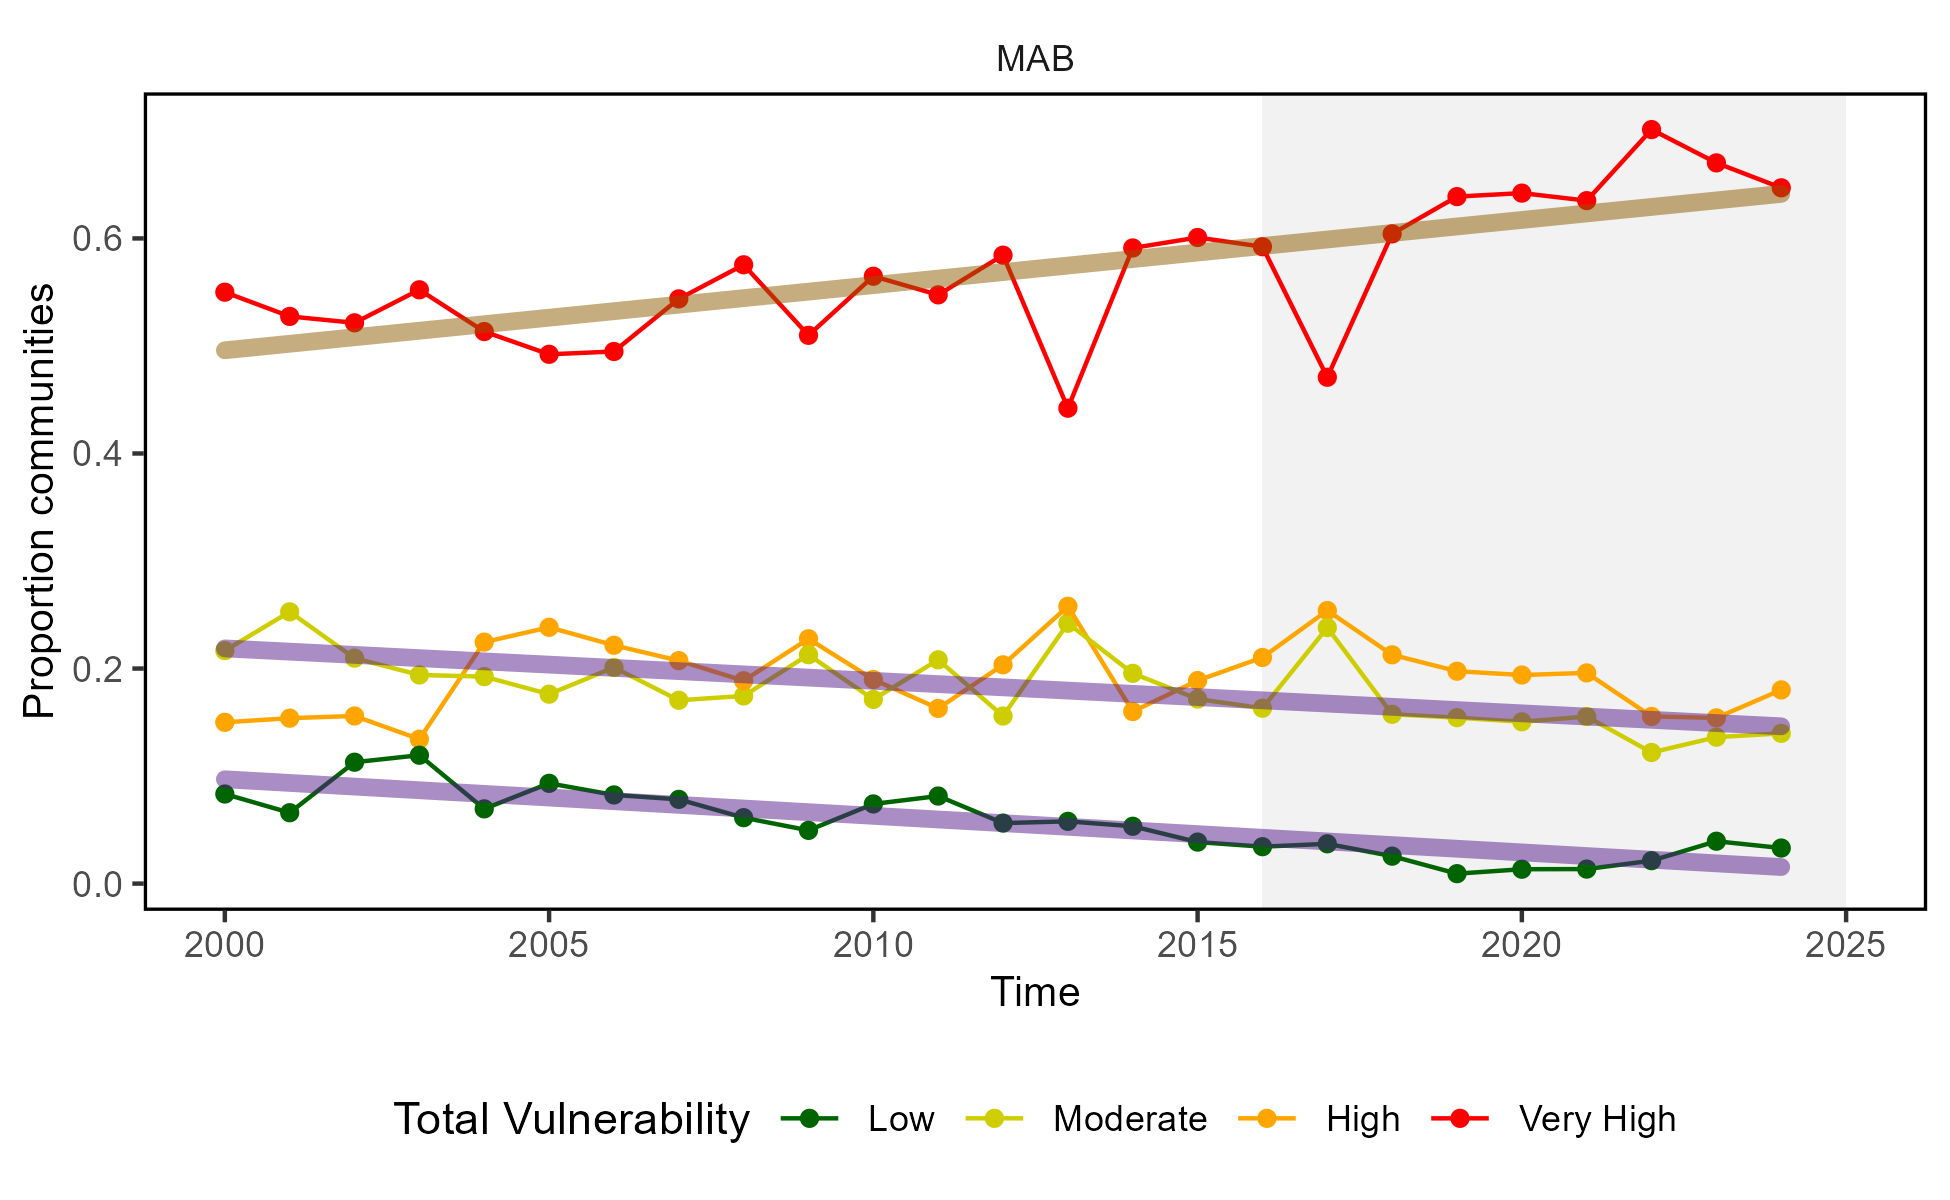
\includegraphics[width=1\linewidth,]{images/MidAtlantic/commvulex_MidAtlantic_2026-03-26} 

}

\caption{Proportion of Mid-Atlantic communities at each revenue environmental variability risk level over time. Total vulnerability ranges from low (green), moderate (yellow), high (orange), to very high (red), with a long-term increase (orange) in very high risk communities and long-term declines (purple) in moderate and low risk communities.}\label{fig:commvulex}
\end{figure}

\subsubsection{Implications}\label{implications-3}

A range of socioeconomic and environmental variability risk concerns are found throughout Mid-Atlantic fishing communities, and the CSVI and CEVRI indicate socio-demographic concerns in the most active commercial Mid-Atlantic fishing ports. Fishing industry participants that utilize more vulnerable ports may be at increased relative risk to changes in fishing patterns due to regulations and/or ecosystem changes.

A majority of Mid-Atlantic communities have high to very high total environmental variability risk based on revenue. Coastal fishing communities are greatly affected by environmental change, both because of their physical location and because of their frequent social, cultural, and economic dependence on fishing. These impacts are expected to become more pressing as changes become more extensive. Changes in \href{https://noaa-edab.github.io/catalog/bottom_temp_insitu.html}{ocean temperature} and \href{https://noaa-edab.github.io/catalog/ocean_acidification.html}{acidification} affecting marine life have the potential to directly impact fisheries and fishery dependent livelihoods.

\subsection{Protected Species}\label{protected-species}

Fishery management objectives for protected species generally focus on reducing threats and on habitat conservation/restoration. Specific actions include managing bycatch to remain below potential biological removal (PBR) thresholds, recovering endangered populations, and monitoring unusual mortality events (UMEs). Protected species include marine mammals protected under the Marine Mammal Protection Act, endangered and threatened species protected under the Endangered Species Act, and migratory birds protected under the Migratory Bird Treaty Act. In the Northeast U.S., endangered/threatened species include Atlantic salmon, Atlantic and shortnose sturgeon, 5 sea turtle species, giant manta ray, oceanic whitetip shark, and 5 baleen whales. Here we report on performance relative to these objectives, as well as how observed and predicted ecosystem changes in the Northeast U.S may impact these objectives in the future.

\subsubsection{Indicators: bycatch, population (adult and juvenile) numbers, mortalities}\label{indicators-bycatch-population-adult-and-juvenile-numbers-mortalities}

The management objective for \href{https://noaa-edab.github.io/catalog/harborporpoise.html}{harbor porpoise} has been met, as the average index (Fig. \ref{fig:harborporpoise}) remains below the current PBR threshold.

\begin{figure}[T]

{\centering 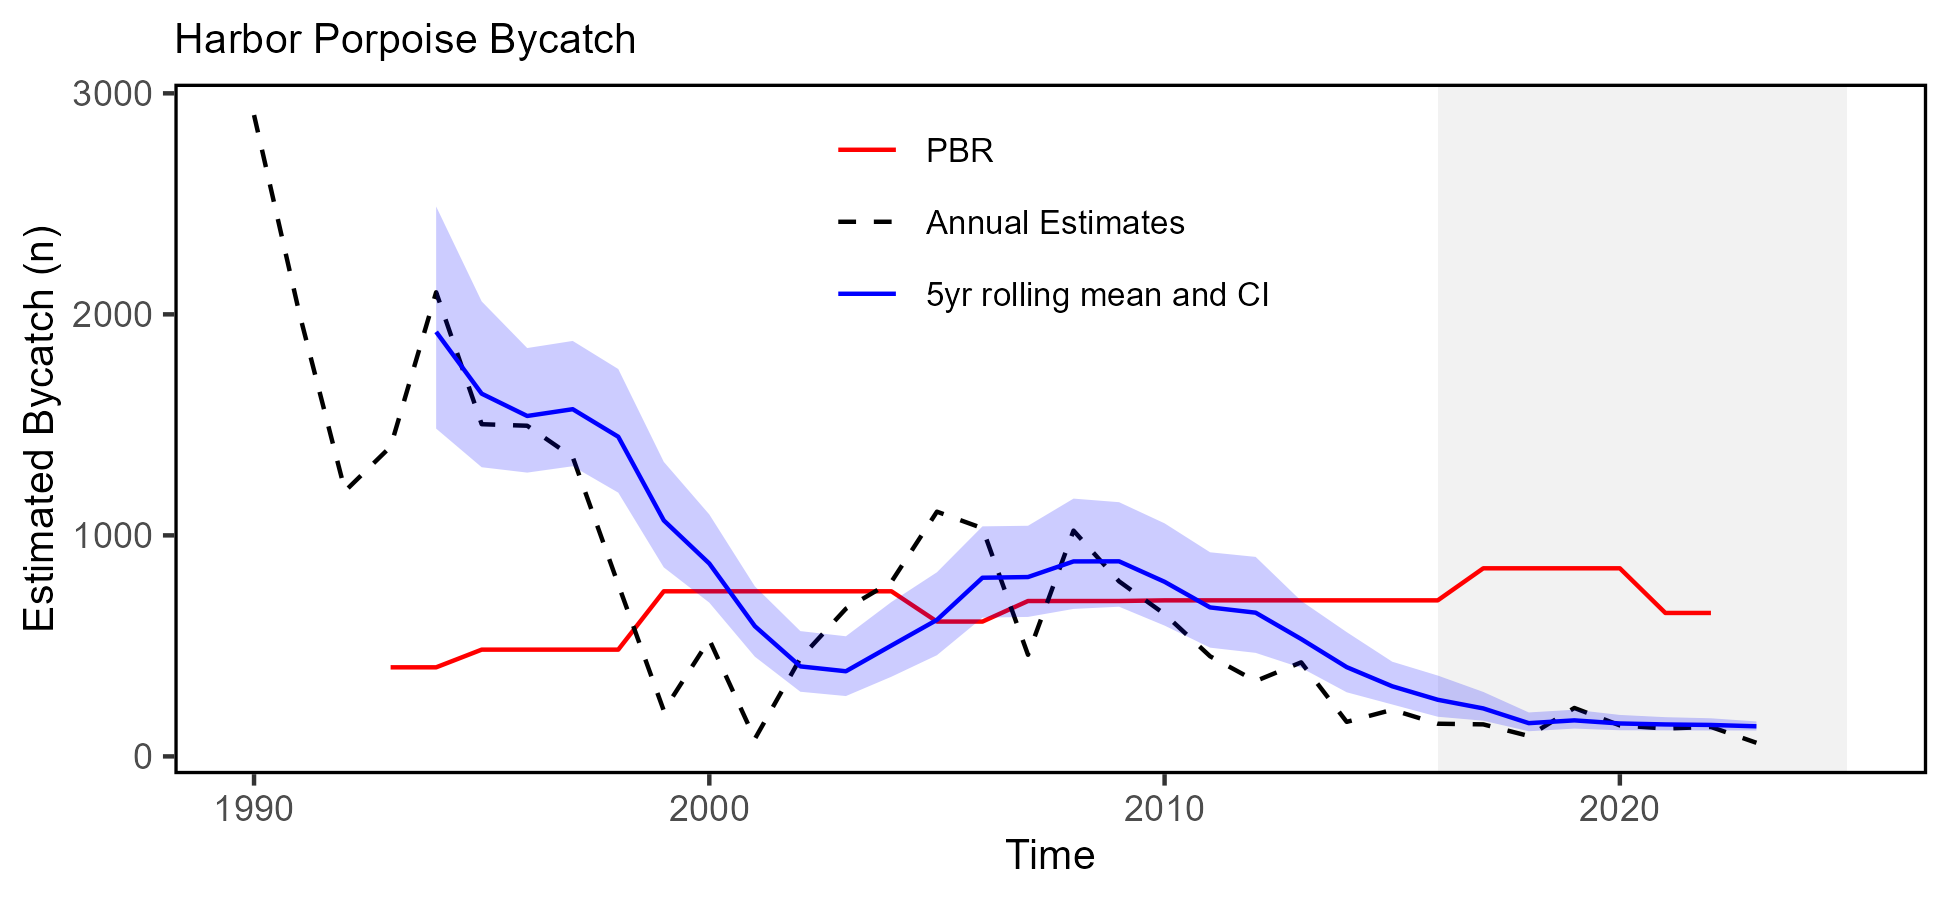
\includegraphics[width=1\linewidth,]{images/BothReports/harborporpoise_BothReports_2026-03-26} 

}

\caption{Harbor porpoise average bycatch estimate for Mid-Atlantic and New England gillnet fisheries (blue, confidence interval shaded) and the potential biological removal (red). The dashed line (black) represents the annual estimated bycatch. }\label{fig:harborporpoise}
\end{figure}

The annual estimate for gray seal bycatch, most of which occurs in New England, has generally declined since 2019, in part driven by declining gillnet landings, although post-2019 estimates have greater uncertainty stemming from low observer coverage. The U.S. and Canadian range-wide PBR for \href{https://noaa-edab.github.io/catalog/grayseal.html}{gray seals} is 12,052. While the PBR for the U.S. portion of this stock was reduced to 756 animals (Fig. \ref{fig:grayseal}), bycatch is unlikely to exceed the range-wide PBR due to incomplete data on anthropogenic mortality and serious injury. Thus the bycatch management objective for gray seals has been met.

\begin{figure}[T]

{\centering 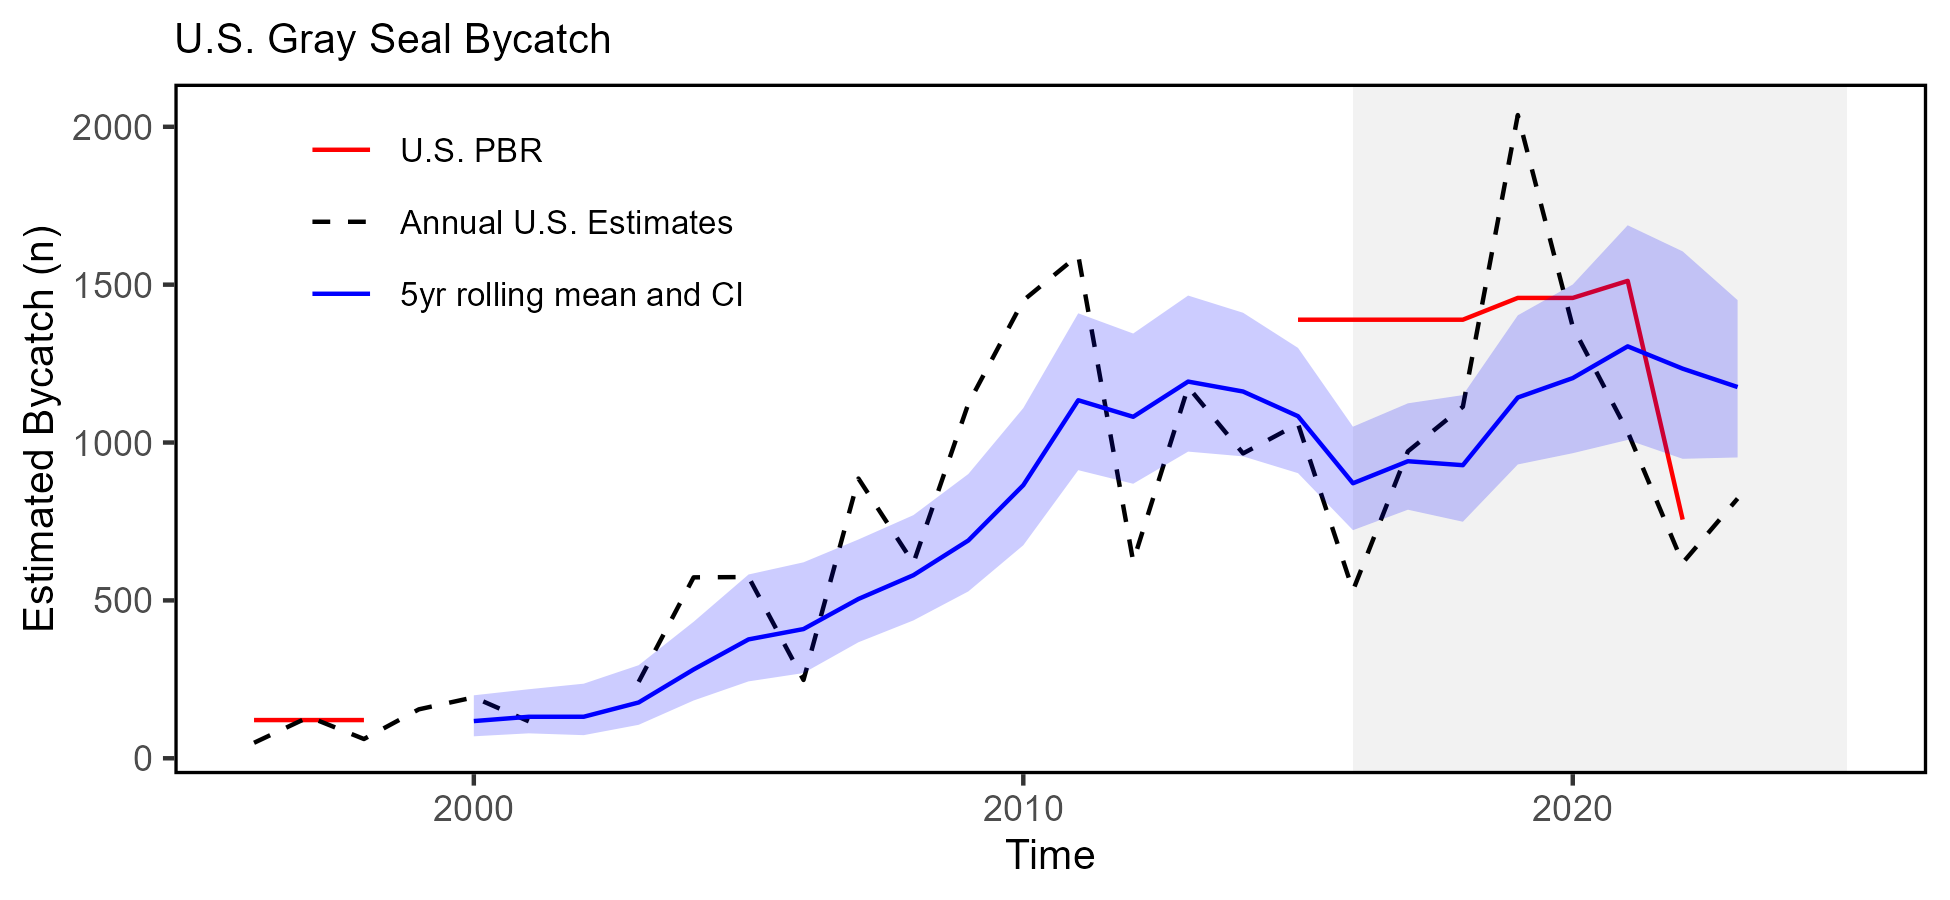
\includegraphics[width=1\linewidth,]{images/BothReports/grayseal_BothReports_2026-03-26} 

}

\caption{Gray seal five-year average bycatch estimate for New England and Mid-Atlantic U.S. gillnet fisheries (blue, with confidence interval shaded) and the potential U.S. biological removal (red). The range-wide potential biological removal (PBR), including both U.S. and Canadian portions of the population, is 12,052 in the draft 2024 SAR. The dashed line (black) represents the annual estimated bycatch.}\label{fig:grayseal}
\end{figure}

The \href{https://noaa-edab.github.io/catalog/narw.html}{North Atlantic right whale population} was on a recovery trajectory until a steep decline after 2010 (Fig. \ref{fig:narw-abundance}). While the right whale population has exhibited slow growth since 2020, it continues to experience annual mortalities above recovery thresholds. Reduced survival rates of adult females lead to diverging abundance trends between sexes. It is estimated that there are approximately 70 reproductively active adult females remaining in the population.

\begin{figure}[T]

{\centering 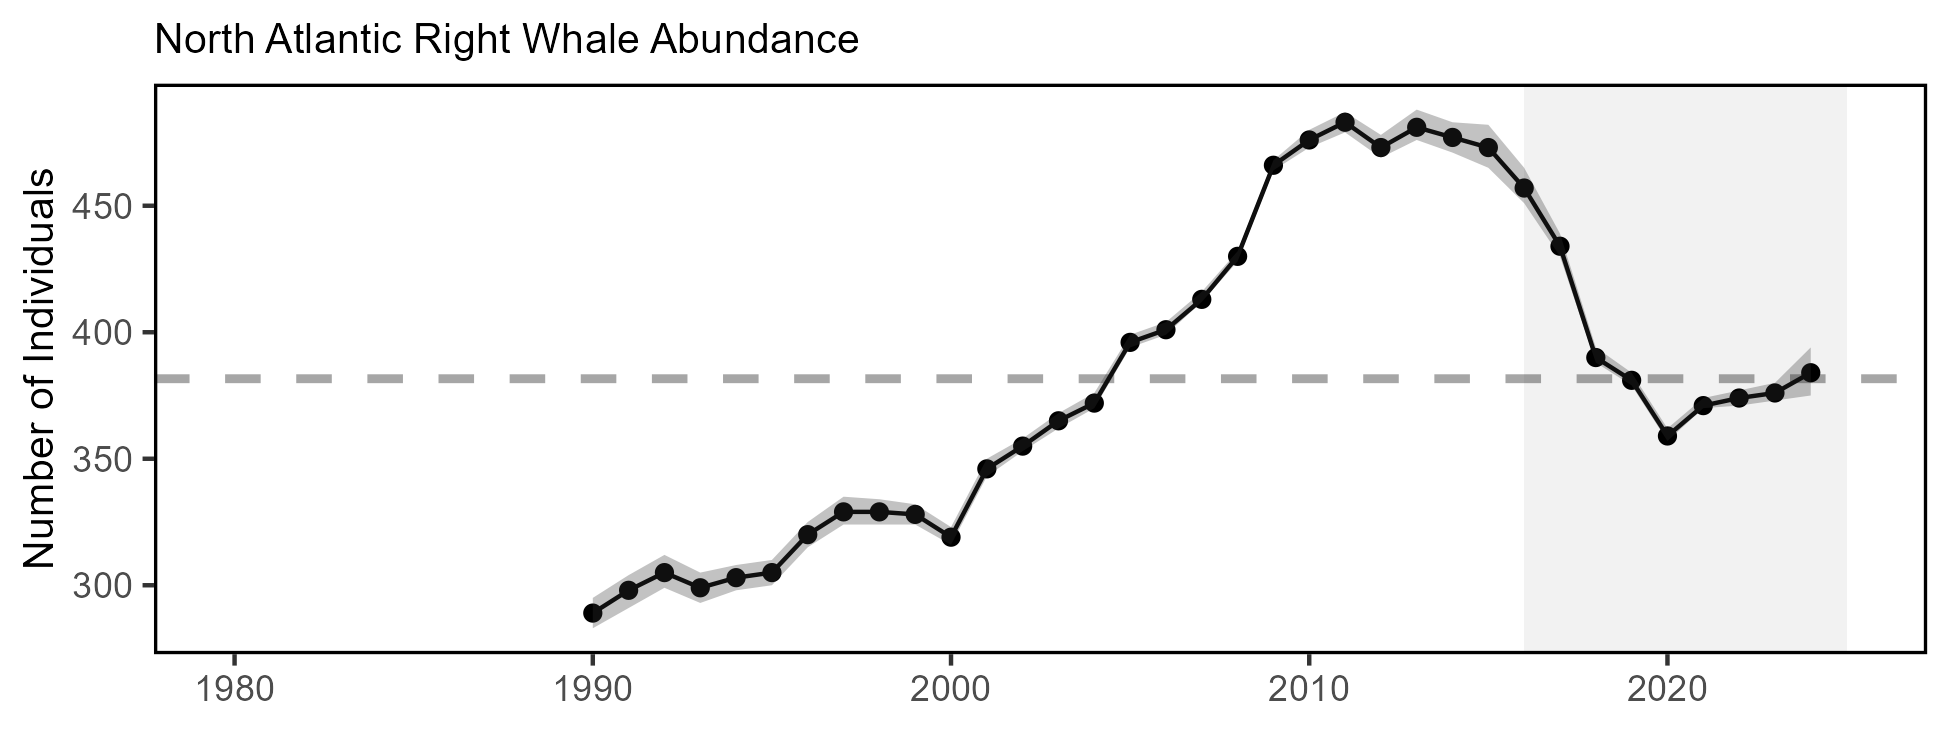
\includegraphics[width=1\linewidth,]{images/BothReports/narw_abundance_BothReports_2026-03-26} 

}

\caption{Estimated North Atlantic right whale abundance on the Northeast Shelf. 95\% confidence interval shaded in gray around the line. }\label{fig:narw-abundance}
\end{figure}

North Atlantic right whale \href{https://noaa-edab.github.io/catalog/narw.html}{calf counts} have generally declined after 2009 to the point of having zero new calves observed in 2018 (Fig. \ref{fig:NARW-calf-abundance}). However, since 2020, calf births have been closer to the long-term average, with 11 calves born in 2025.

\begin{figure}[T]

{\centering 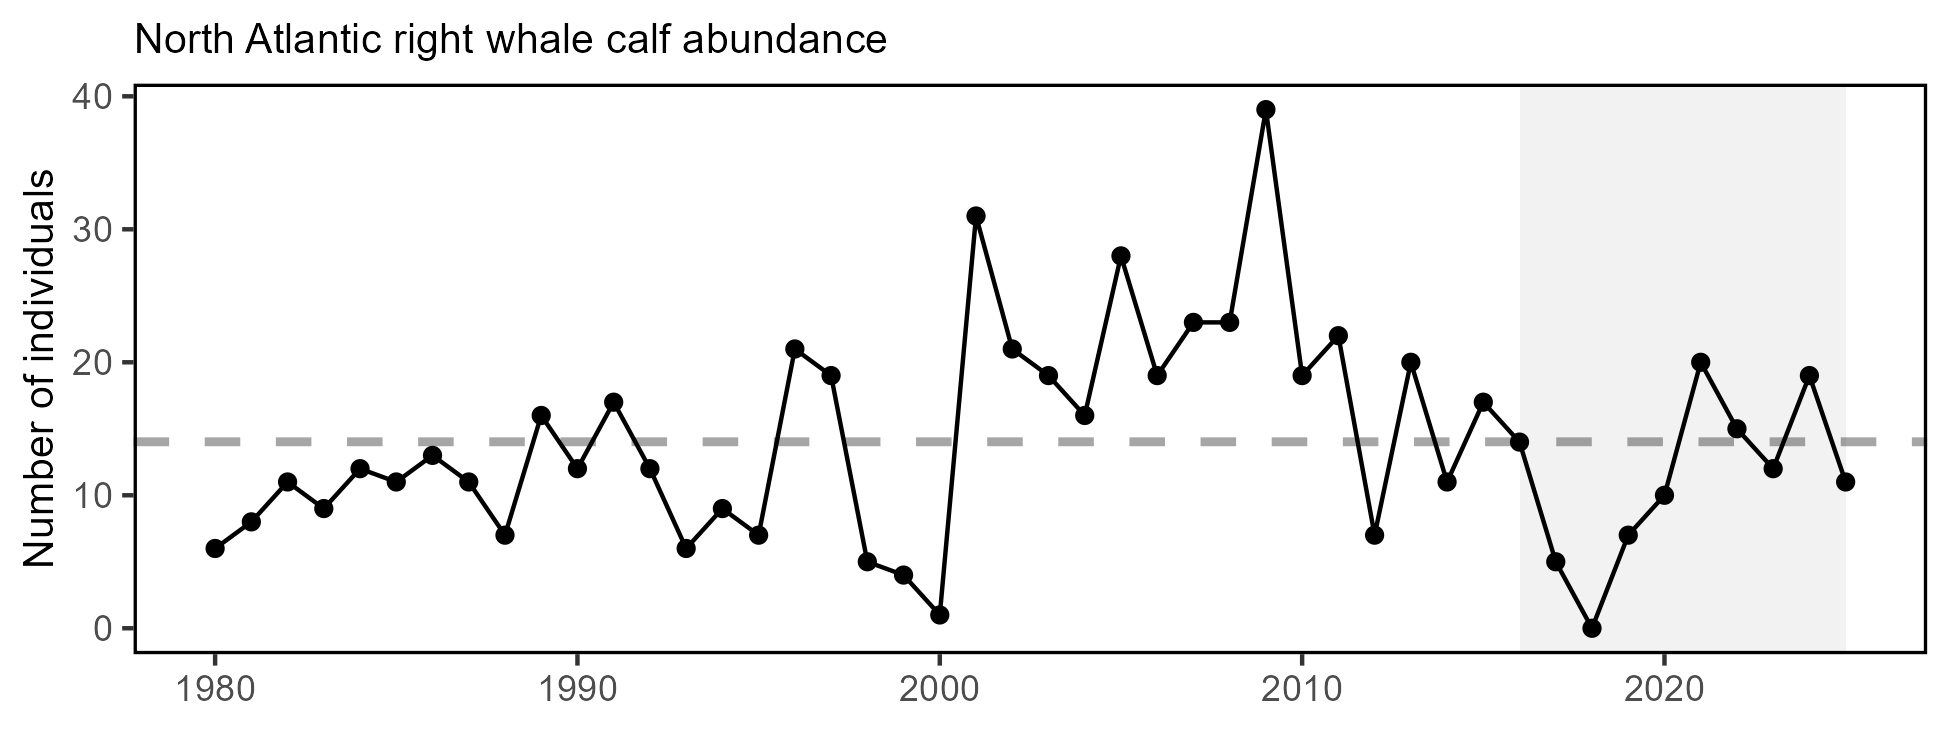
\includegraphics[width=1\linewidth,]{images/BothReports/narw_calves_BothReports_2026-03-26} 

}

\caption{Number of North Atlantic right whale calf births since 1980. }\label{fig:NARW-calf-abundance}
\end{figure}

Human interaction from entanglements or vessel strikes remains the primary cause of death in an ongoing North Atlantic right whale Unusual Mortality Event (UME) since 2017. As of January 5, 2026, \href{https://www.fisheries.noaa.gov/national/marine-life-distress/2017-2026-north-atlantic-right-whale-unusual-mortality-event}{the UME} includes 168 individual whales: 41 confirmed mortalities (19 US; 22 Canada), 40 serious injuries, and 87 sublethal injuries or illnesses. Recent research suggests that many mortalities go unobserved and the true number of mortalities are about three times the count of the observed mortalities.

There is an ongoing UME for humpback whales (2016-present) and Atlantic minke whales (2018-present); suspected causes include human interactions. A UME for Northeast pinnipeds that began in 2018 for infectious disease is non-active pending closure as of February 2026.

\subsubsection{Implications}\label{implications-4}

Bycatch management measures have been implemented to maintain bycatch below PBR thresholds. The downward trend in harbor porpoise bycatch could also be due to a decrease in harbor porpoise abundance in U.S. waters, reducing their overlap with fisheries, and a decrease in gillnet effort. The increasing trend in 5-year average gray seal bycatch may be related to an increase in the gray seal population (\href{https://noaa-edab.github.io/catalog/seal_pups.html}{U.S. pup counts}; Fig. \ref{fig:seals}), supported by the dramatic rise over the last three decades in observed numbers of gray seal pups born at U.S. breeding sites plus an increase in adult seals at the breeding sites, some of which are supplemented by Canadian adults.

Strong evidence exists to suggest that interactions between right whales and both the fixed gear fisheries in the U.S. and Canada and vessel strikes in the U.S. are contributing substantially to the decline of the species. Further, right whale distribution has changed since 2010. \href{https://noaa-edab.github.io/catalog/narw.html}{Recent research} suggests that recent climate driven changes in ocean circulation have resulted in right whale distribution changes driven by increased warm water influx through the Northeast Channel, which has reduced the \href{https://noaa-edab.github.io/catalog/preyfield_energy.html}{primary right whale prey} (the copepod \emph{Calanus finmarchicus}) in the central and eastern portions of the Gulf of Maine. Additional potential stressors include offshore wind development, which overlaps with important habitat areas used year-round by right whales, including mother and calf migration corridors and foraging habitat. Additional information can be found in the \hyperref[other-ocean-uses-offshore-wind]{offshore wind risks section}.

The UMEs are under investigation and are likely the result of multiple drivers. For all large whale UMEs, human interaction appears to have contributed to increased mortalities, although investigations are not complete.

\href{https://journals.plos.org/plosone/article?id=10.1371/journal.pone.0290643}{A climate vulnerability assessment} is published for Atlantic and Gulf marine mammal populations.

\newpage

\subsection{Stability}\label{stability}

This year, we have updated the definition of stability for fisheries and ecosystems to represent how consistent we expect the system to be over time. Three components of stability are considered for the purpose of this report: volatility, adaptive capacity, and a shift from baseline. Volatility is a measure of predictability, where volatile conditions indicate that future years are more likely to be different than the recent past. Adaptive capacity refers to a system's ability to respond to changes without fundamentally changing its composition or structure. A shift from baseline refers to a systemic shift in a system towards a new status, where prior conditions may no longer be the norm. Measures of volatility are currently being developed. Therefore, we assess fisheries and ecosystem stability as ``stable'' if there is no notable change in adaptive capacity or shifts from a historic baseline, and ``not stable'' if there are changes in either of these components.

This year, we have updated the definition of stability for fisheries and ecosystems as a measure of how consistent we expect the system to be over time. Three components of stability are considered for the purpose of this report: volatility, adaptive capacity, and a shift from baseline. Volatility is a measure of predictability, where volatile conditions indicate that future years are more likely to be different than the recent past. Adaptive capacity refers to a system's ability to respond to changes without fundamentally changing its composition or structure. A shift from baseline refers to a systemic shift in a system towards a new status, where prior conditions may no longer be the norm. Measures of volatility are currently being developed. Therefore, we assess fisheries and ecosystem stability as ``stable'' if there is no notable change in adaptive capacity or shifts from a historic baseline, and ``not stable'' if there are changes in either of these components.

\paragraph{Fishery Stability}\label{fishery-stability}

Indicators suggest that Mid-Atlantic fisheries have broadly shifted from the historic baseline. Commercial fishery fleet count has declined while fleet revenue diversity has been stable over time in the MAB, but current fleet revenue diversity is above the long-term average (Fig. \ref{fig:comm-div-fleet}). This indicates that the commercial fleet composition has changed, but the portfolio of species targeted is similar over time (Fig. \ref{fig:commercial-div-species-div}). \href{https://noaa-edab.github.io/catalog/effective_sweptarea.html}{Revenue per unit effort} remains steady or increasing over time for most gear types, indicating financial viability of current fishing operations. Target species such as Atlantic mackerel and quahog have had reduced catch limits in recent years, resulting in reduced landings in these fisheries, and a decline in scallop catch within the MAB has severely reduced the total revenue generated in the region. Because non-MAFMC managed landings and revenue have declined, a larger share of the regional landings and revenue come from Council-managed fisheries.

The \href{https://noaa-edab.github.io/catalog/crew_survey.html}{Crew Survey} shows that specific aspects pertaining to sustainability and resilience of the fishing lifestyle are declining: predictability of earnings, the amount of time away from home, the physical fatigue of the job, and the personal health impacts have all been cited as dissatisfaction rates increase. Overall job satisfaction remains relatively stable over time, but unveils vulnerability as additional survey results show an aging population, particularly an increase in the 55+ crew cohort, and fewer individuals entering the fishery. This suggests a reduced capacity for Mid-Atlantic commercial fisheries to adapt to future uncertainties and change. New \href{https://noaa-edab.github.io/catalog/communities_at_sea.html}{Communities at Sea} indicators that assess fishing communities' ability to adapt to change are in development and will provide additional fishing industry indicators in future reports.

Despite reduced \href{https://noaa-edab.github.io/catalog/recdat.html}{recreational landings} (Fig. \ref{fig:rec-landings}), the number of recreational trips is near average (Fig. \ref{fig:rec-op}), suggesting a shift to catch-and-release fishing. Billfish (i.e., white marlin) catch-and-release was especially high, possibly due to shifting effort due to the closure of the recreational bluefin tuna fishery in August 2025. Shark and large sport fish regulations and environmental conditions, among other circumstances, may also contribute to reduced recreational landings. As noted above, \href{https://noaa-edab.github.io/catalog/recdat.html}{recreational fleet effort diversity} is declining (Fig. \ref{fig:rec-div}), suggesting a shift in modes of recreational fishery participation. The Mid-Atlantic has experienced a contraction of the party and charter sectors, with more recreational angling occurring from shore. Recreational species catch diversity has no long-term trend and has been at or above the long-term average since 2016 (Fig. \ref{fig:recdat-div-catch}), indicating that anglers continue to catch a mix of species.

\begin{figure}[T]

{\centering 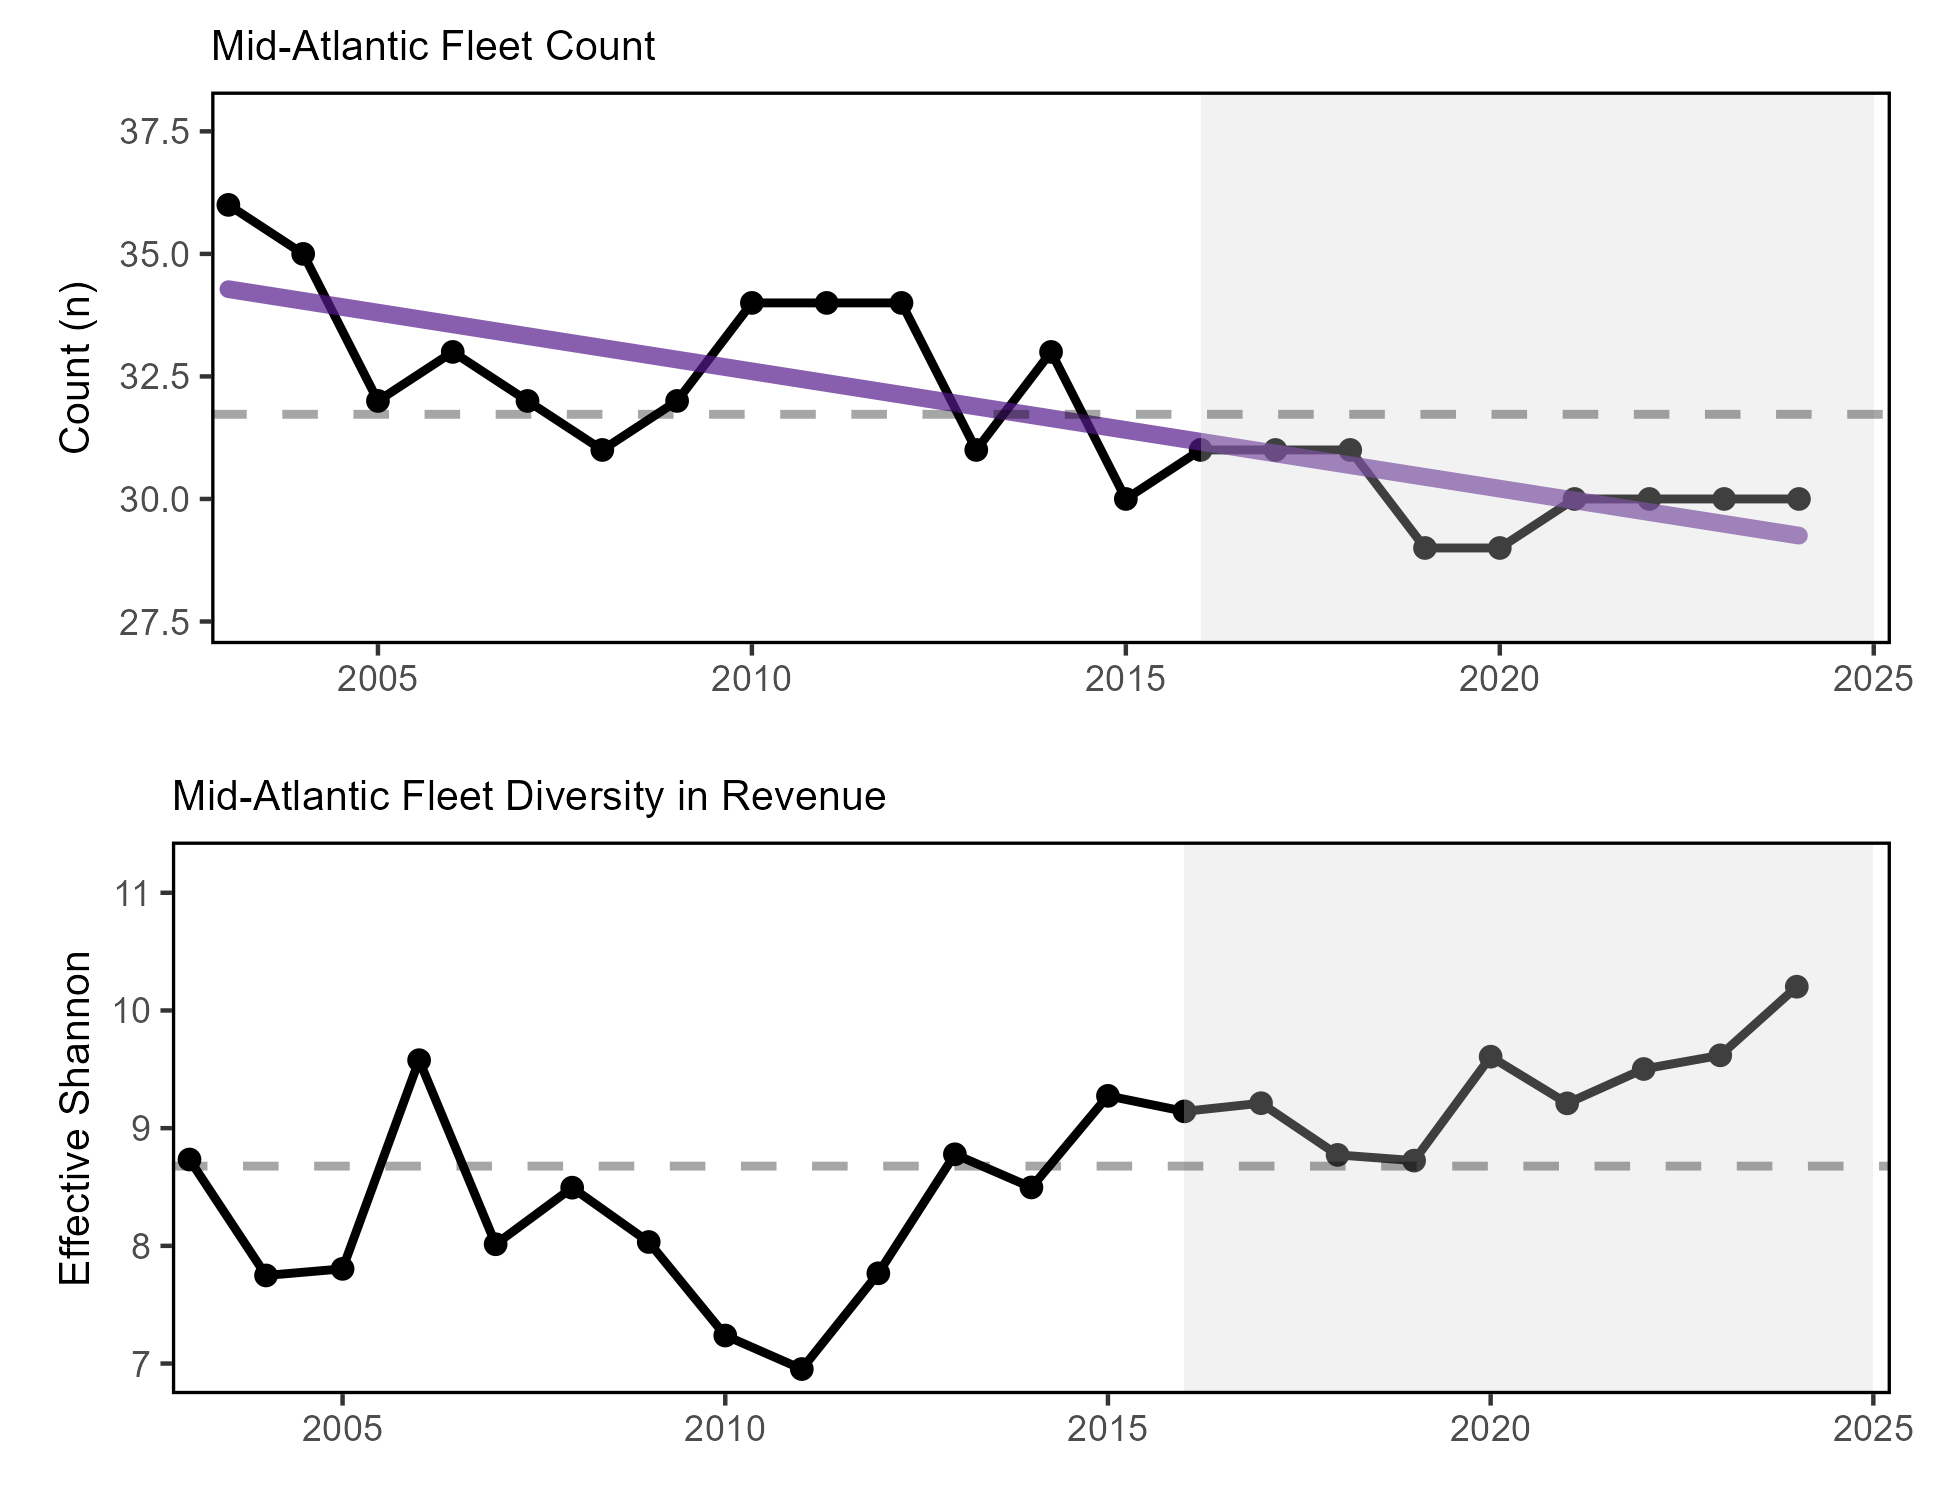
\includegraphics[width=1\linewidth,]{images/MidAtlantic/comm_div_fleet_MidAtlantic_2026-03-26} 

}

\caption{Commercial fleet count (top) and fleet diversity in revenue (bottom) in the Mid-Atlantic  with significant long-term decline in fleet count (purple line).}\label{fig:comm-div-fleet}
\end{figure}

\begin{figure}[T]

{\centering 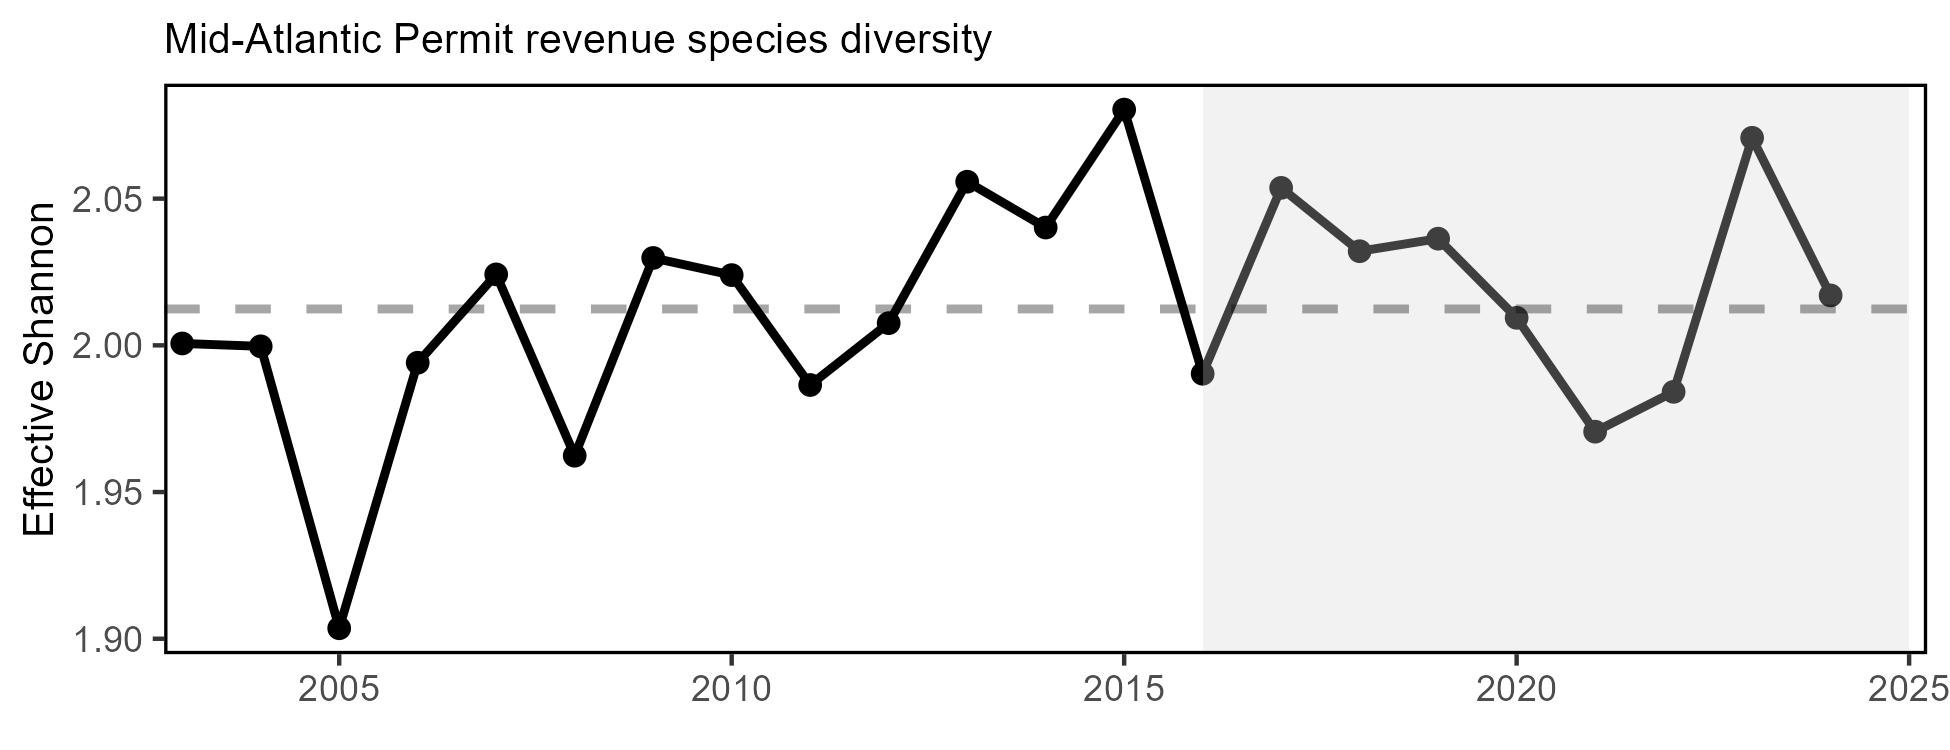
\includegraphics[width=1\linewidth,]{images/MidAtlantic/commercial_div_species_div_MidAtlantic_2026-03-26} 

}

\caption{Species revenue diversity (permit-level species effective Shannon index) in the Mid-Atlantic.}\label{fig:commercial-div-species-div}
\end{figure}

\begin{figure}[T]

{\centering 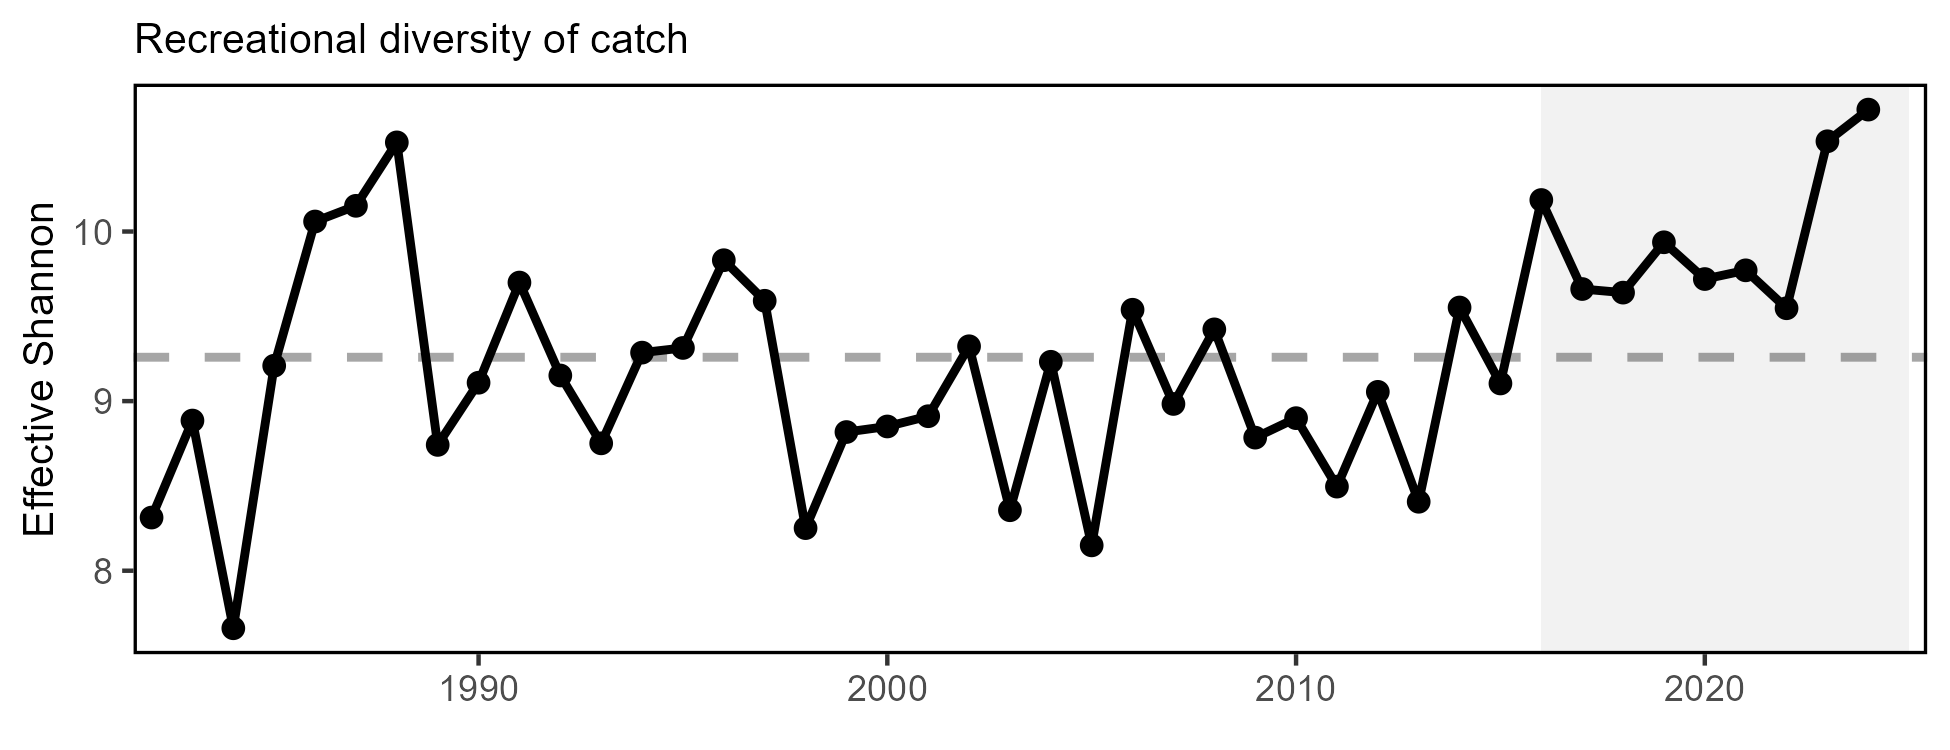
\includegraphics[width=1\linewidth,]{images/MidAtlantic/recdat_div_catch_MidAtlantic_2026-03-26} 

}

\caption{Diversity of recreational catch in the Mid-Atlantic. Derived from NOAA Fisheries Marine Recreational Information Program's Catch Time Series Query.}\label{fig:recdat-div-catch}
\end{figure}

\paragraph{Ecological Stability}\label{ecological-stability}

Long-term changes in biological processes suggest the Mid-Atlantic ecosystem is experiencing a systemic shift. Total annual \href{https://noaa-edab.github.io/catalog/chl_pp.html}{primary production}, a measure of the total amount of carbon (i.e., energy) produced by phytoplankton per year, has no clear trend (Fig. \ref{fig:totpp}), suggesting stability in energy at the base of the food web. However, we are monitoring for shifts in the phytoplankton community, which can affect the amount of primary production available to higher trophic levels. \href{https://noaa-edab.github.io/catalog/zoo_diversity.html}{Zooplankton diversity} is increasing in the MAB, and measures of zooplankton community composition also indicate a long-term shift in \href{https://noaa-edab.github.io/catalog/zoo_community.html}{zooplankton communities} (Fig. \ref{fig:zoo-community}). Together, these indicators show a gradual but systemic change in lower trophic levels towards a community with a higher proportion of euphausiids and less dominated by copepods, which would not be expected in a stable ecosystem.

There are long-term increases in the biomass of the euphausid, benthivore, and benthos \href{https://noaa-edab.github.io/catalog/aggregate_biomass.html}{guilds} (Fig. \ref{fig:nefsc-biomass-mab}). These lower trophic groups have similar roles within the ecosystem and these changes indicate a shift towards an ecosystem with a higher representation of those functional groups. \href{https://noaa-edab.github.io/catalog/exp_n.html}{Adult fish diversity}, the expected number of species in a standard number of individuals sampled from the NEFSC bottom trawl survey, had no trend when the Albatross vessel was used for sampling, but shows a short-term declining trend since switching to the Bigelow vessel in 2008. However, the expected number of species observed is currently within one standard deviation from most historic estimates (Fig. \ref{fig:exp-n}). This suggests that biomass increases in some guilds is due to an overall producivity increase rather than an influx of new species.

\begin{figure}[T]

{\centering 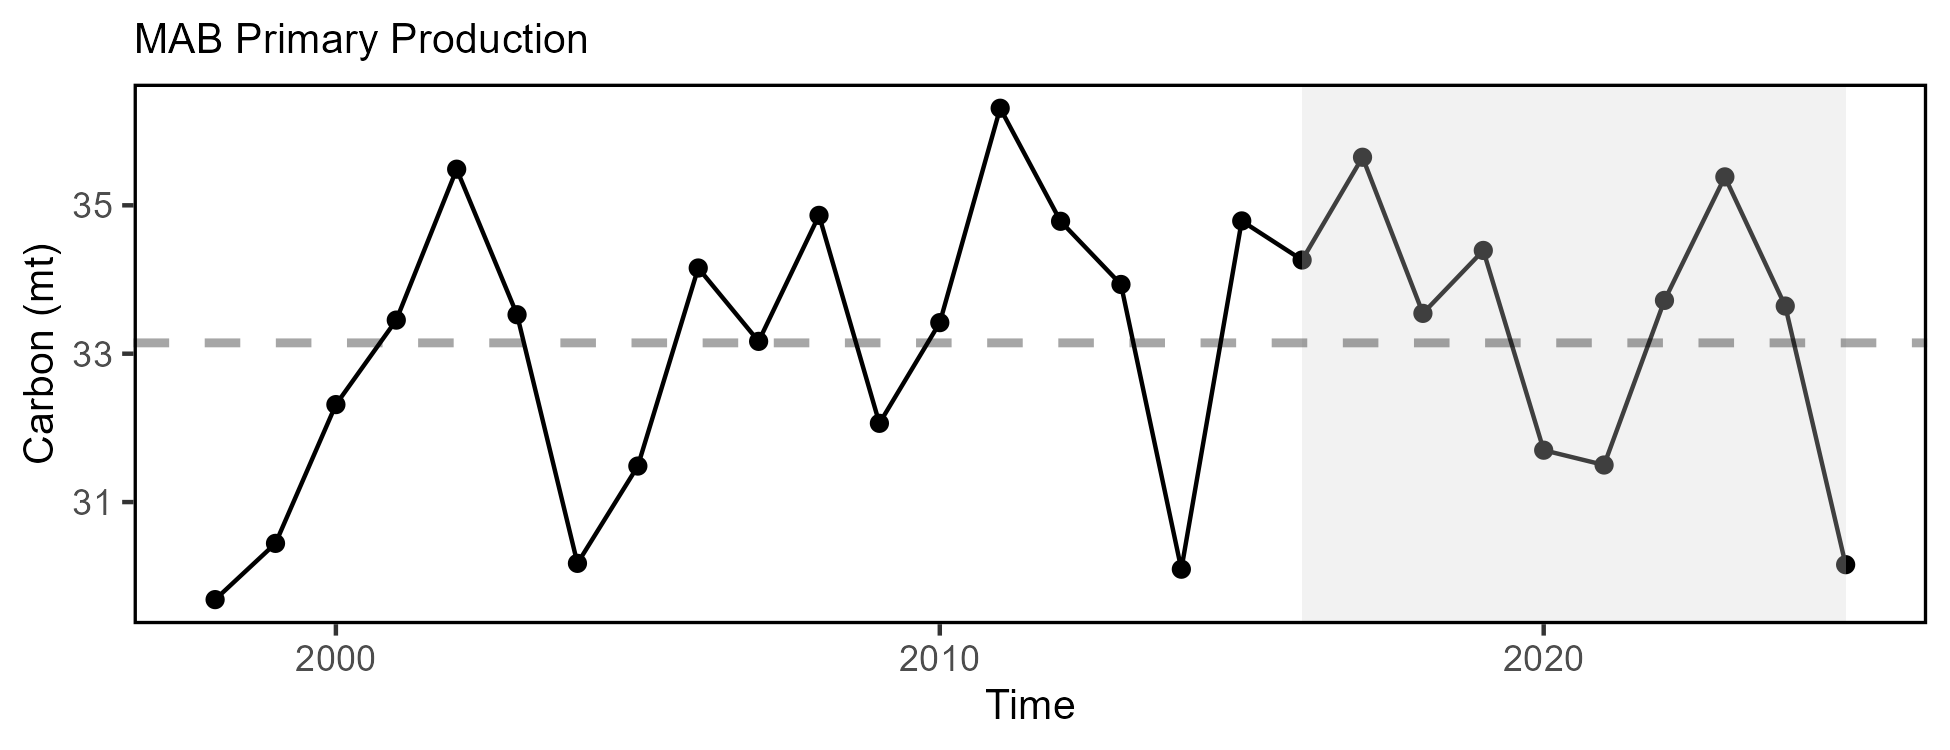
\includegraphics[width=1\linewidth,]{images/MidAtlantic/totpp_MidAtlantic_2026-03-26} 

}

\caption{Total areal annual primary production for the Mid-Atlantic Bight. The dashed line represents the long-term (1998-2025) annual mean.}\label{fig:totpp}
\end{figure}

\begin{figure}[T]

{\centering 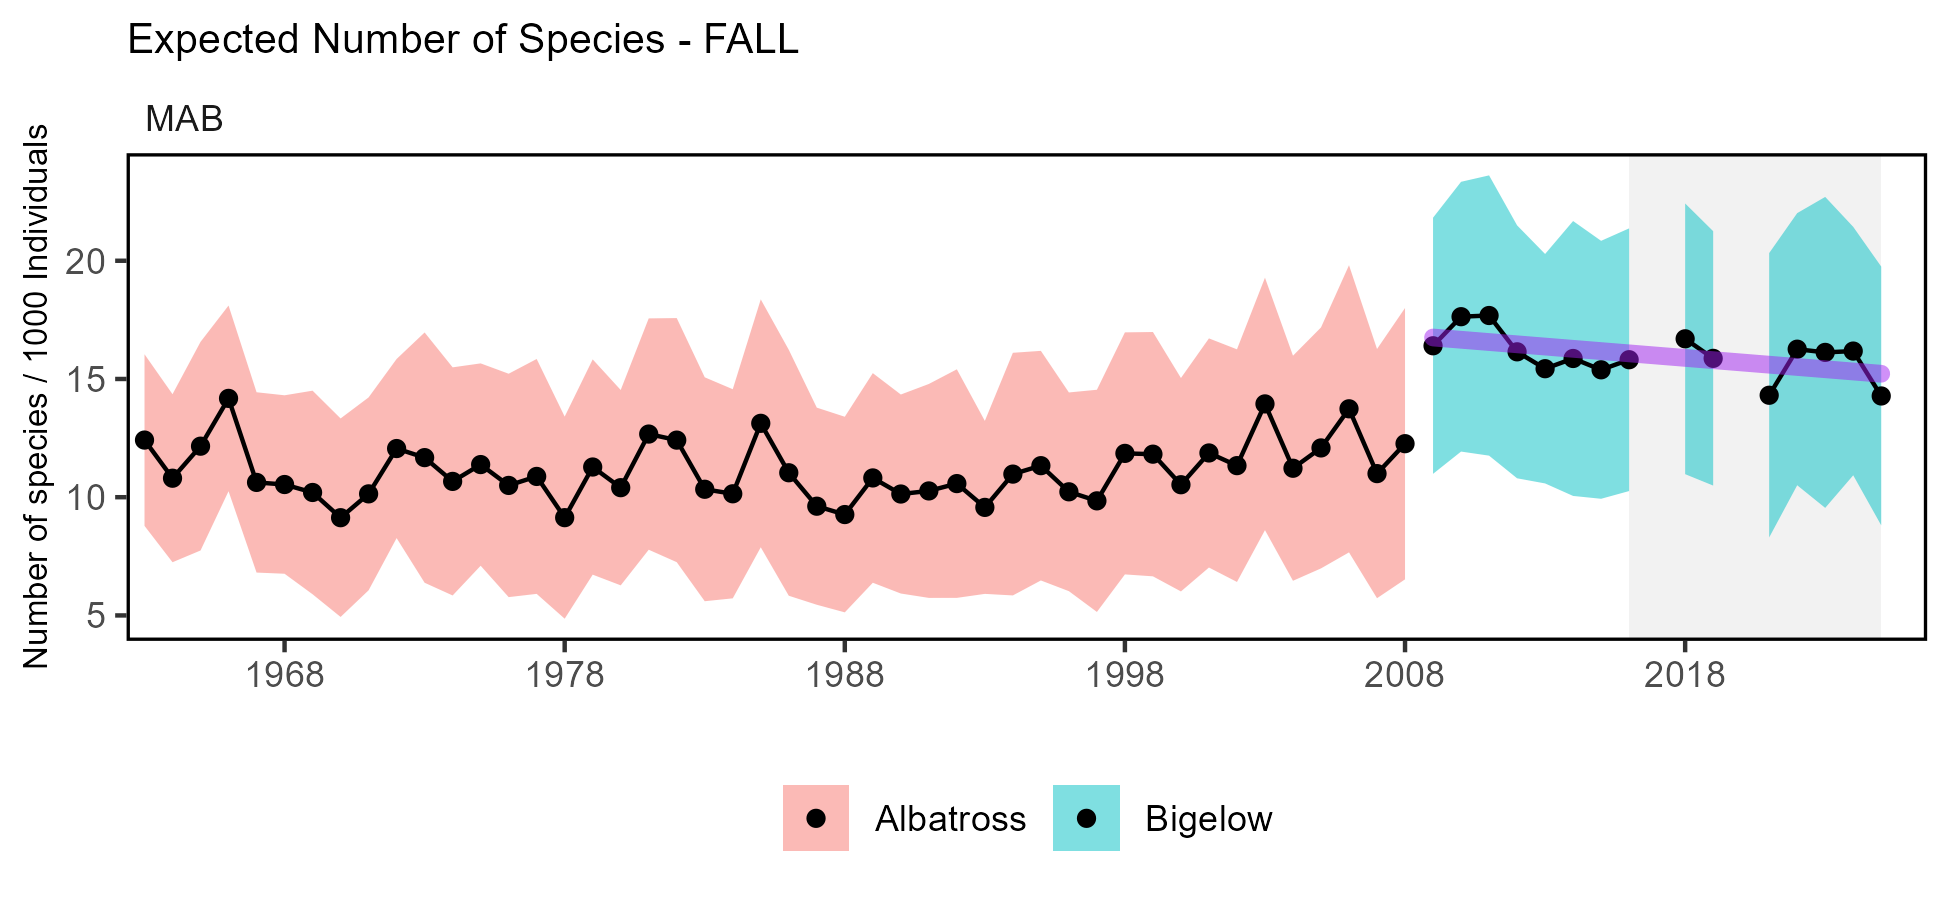
\includegraphics[width=1\linewidth,]{images/MidAtlantic/exp_n_MidAtlantic_2026-03-26} 

}

\caption{Adult fish diversity in the Mid-Atlantic Bight, based on expected number of species in a standard number of individuals. Results from survey vessels Albatross (red) and Bigelow (blue) are reported separately due to catchability differences. A long-term significant decrease is present in the Bigelow time series (purple).}\label{fig:exp-n}
\end{figure}

\begin{figure}[T]

{\centering 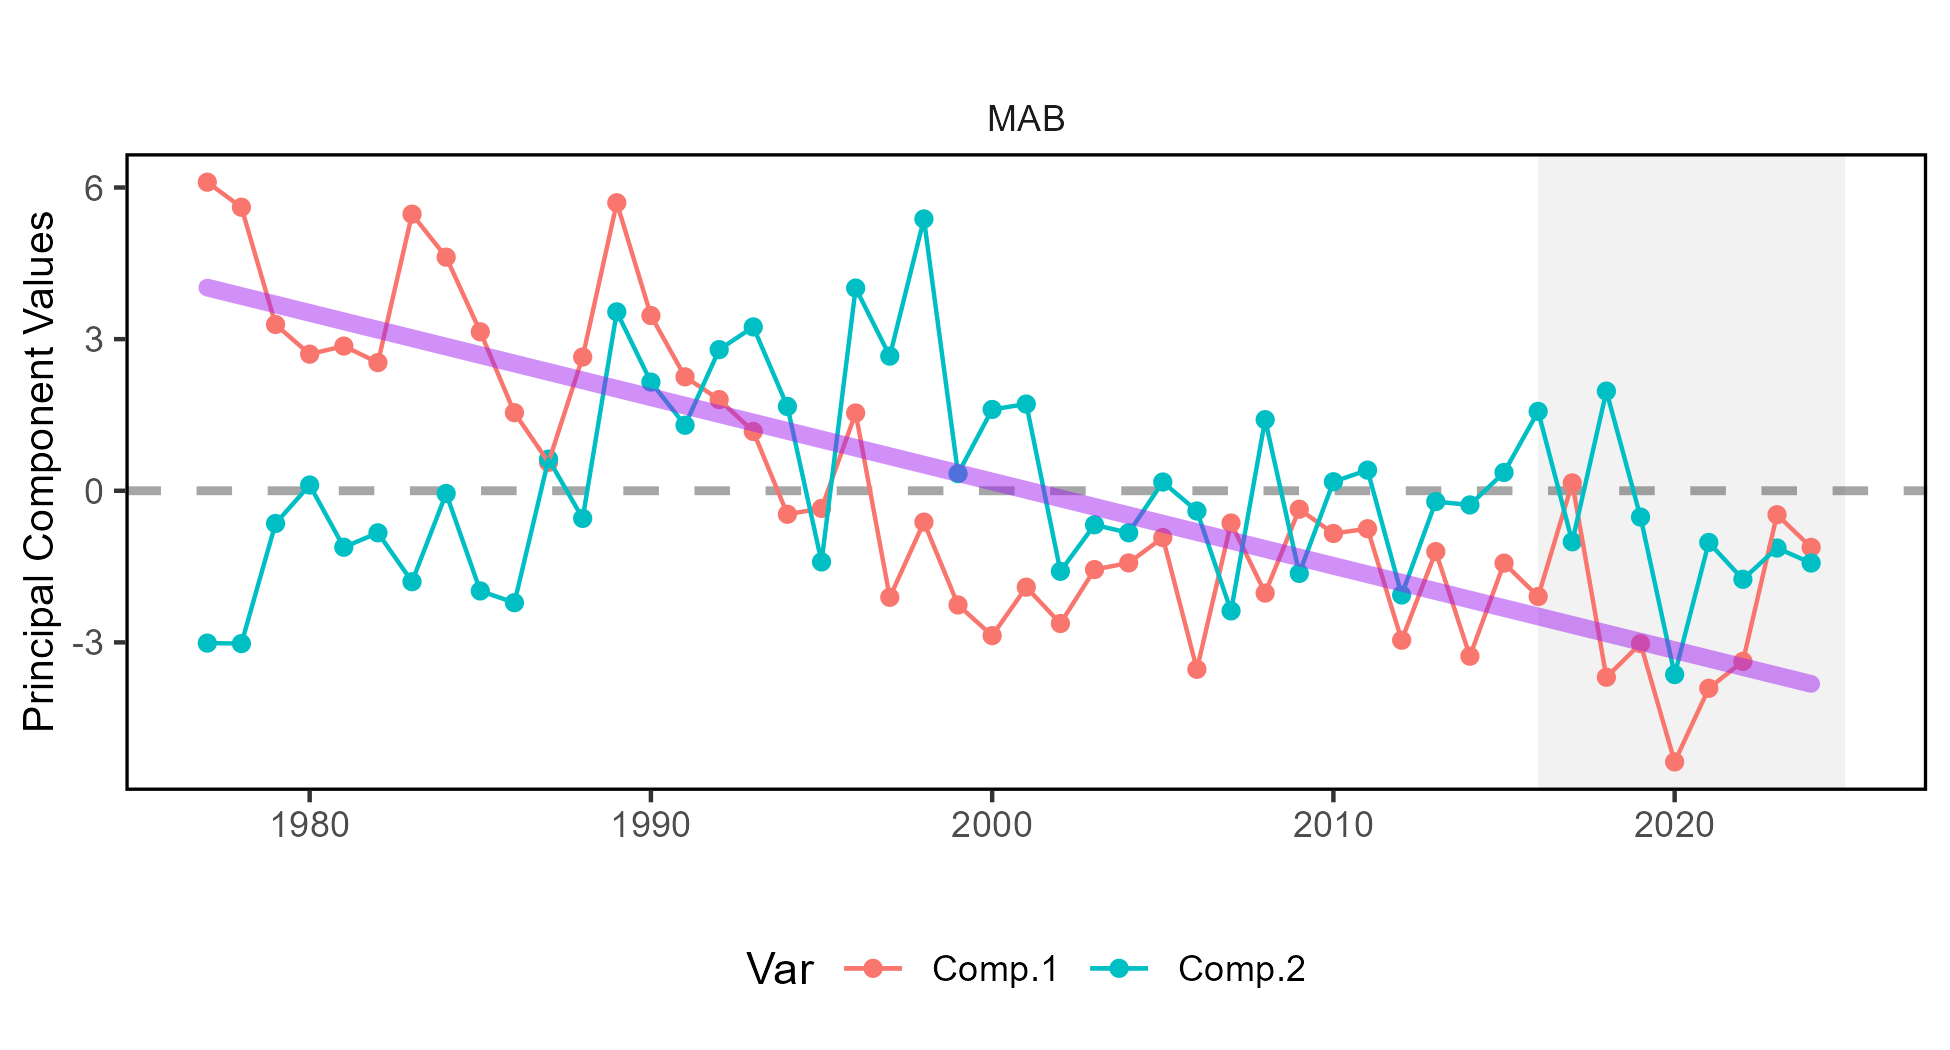
\includegraphics[width=1\linewidth,]{images/MidAtlantic/zoo_community_MidAtlantic_2026-03-26} 

}

\caption{Principal component analysis of zooplankton community composition in the Mid-Atlantic Bight. Lines show the first two principal components (colors). The long-term declining trendline (purple) is associated with the first principal component. This trend is driven by an increasing abundance of sea butterflies, hyperiid amphipods, echinoderm larvae, arrow worms, and the copepod \textit{Calanus minor}, and a decreasing abundance of the copepods \textit{Pseudocalanus spp.}, \textit{Centropages hamatus}, \textit{Acartia spp.}, and \textit{Temora longicornis}.}\label{fig:zoo-community}
\end{figure}

\href{https://noaa-edab.github.io/catalog/finfish_traits.html}{Functional traits}, such as length at maturity, maximum body size, and fecundity, serve to synthesize change in complex, diverse communities by looking beyond species-specific trends. Furthermore, shifts in functional trait distributions for the fish community can indicate changes in ecosystem-scale resilience. There is evidence of long-term change in trait distributions in the MAB, particularly in the fall season (Fig. \ref{fig:traits-k}, \ref{fig:traits-tl}). The fall finfish community in the MAB is showing long-term shifts towards faster life history strategies with lower trophic levels, smaller offspring, younger age and shorter length at maturity, and faster growth rates. This indicates shifts in a system increasingly composed of smaller, fast-growing species. The long-term trends in the spring season are, however, more equivocal, with some evidence in shifts towards slower life history strategies, including larger length-at-maturity and offspring size. The lack of trend in finfish diversity suggests that these changes in fish communities are not due to a change in the total number of species.

\begin{figure}[T]

{\centering 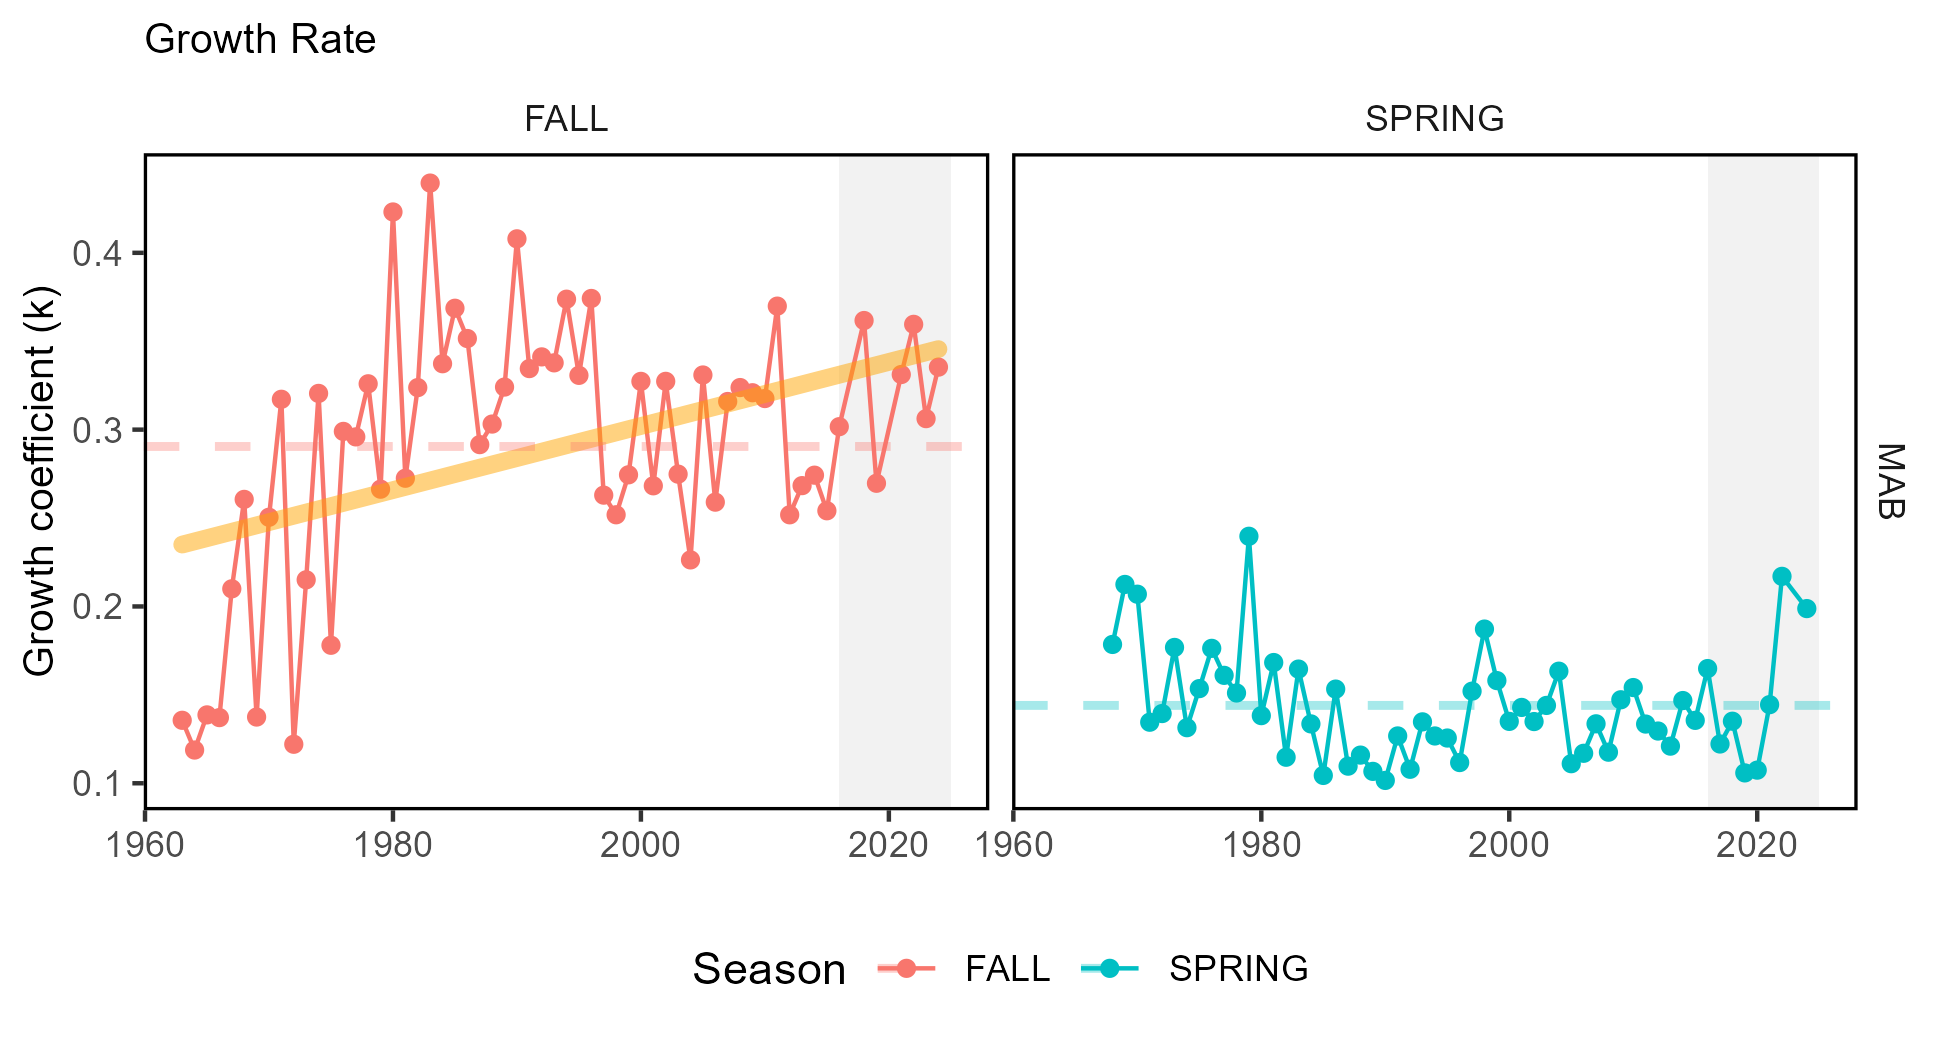
\includegraphics[width=1\linewidth,]{images/MidAtlantic/traits_k_MidAtlantic_2026-03-27} 

}

\caption{Fish community functional traits (growth rate) in the Mid-Atlantic Bight based on Fall (red) and Spring (blue) survey data with a significant long-term increase (orange) present in the fall. Dashed lines represent the long-term annual mean for each survey.}\label{fig:traits-k}
\end{figure}

\begin{figure}[T]

{\centering 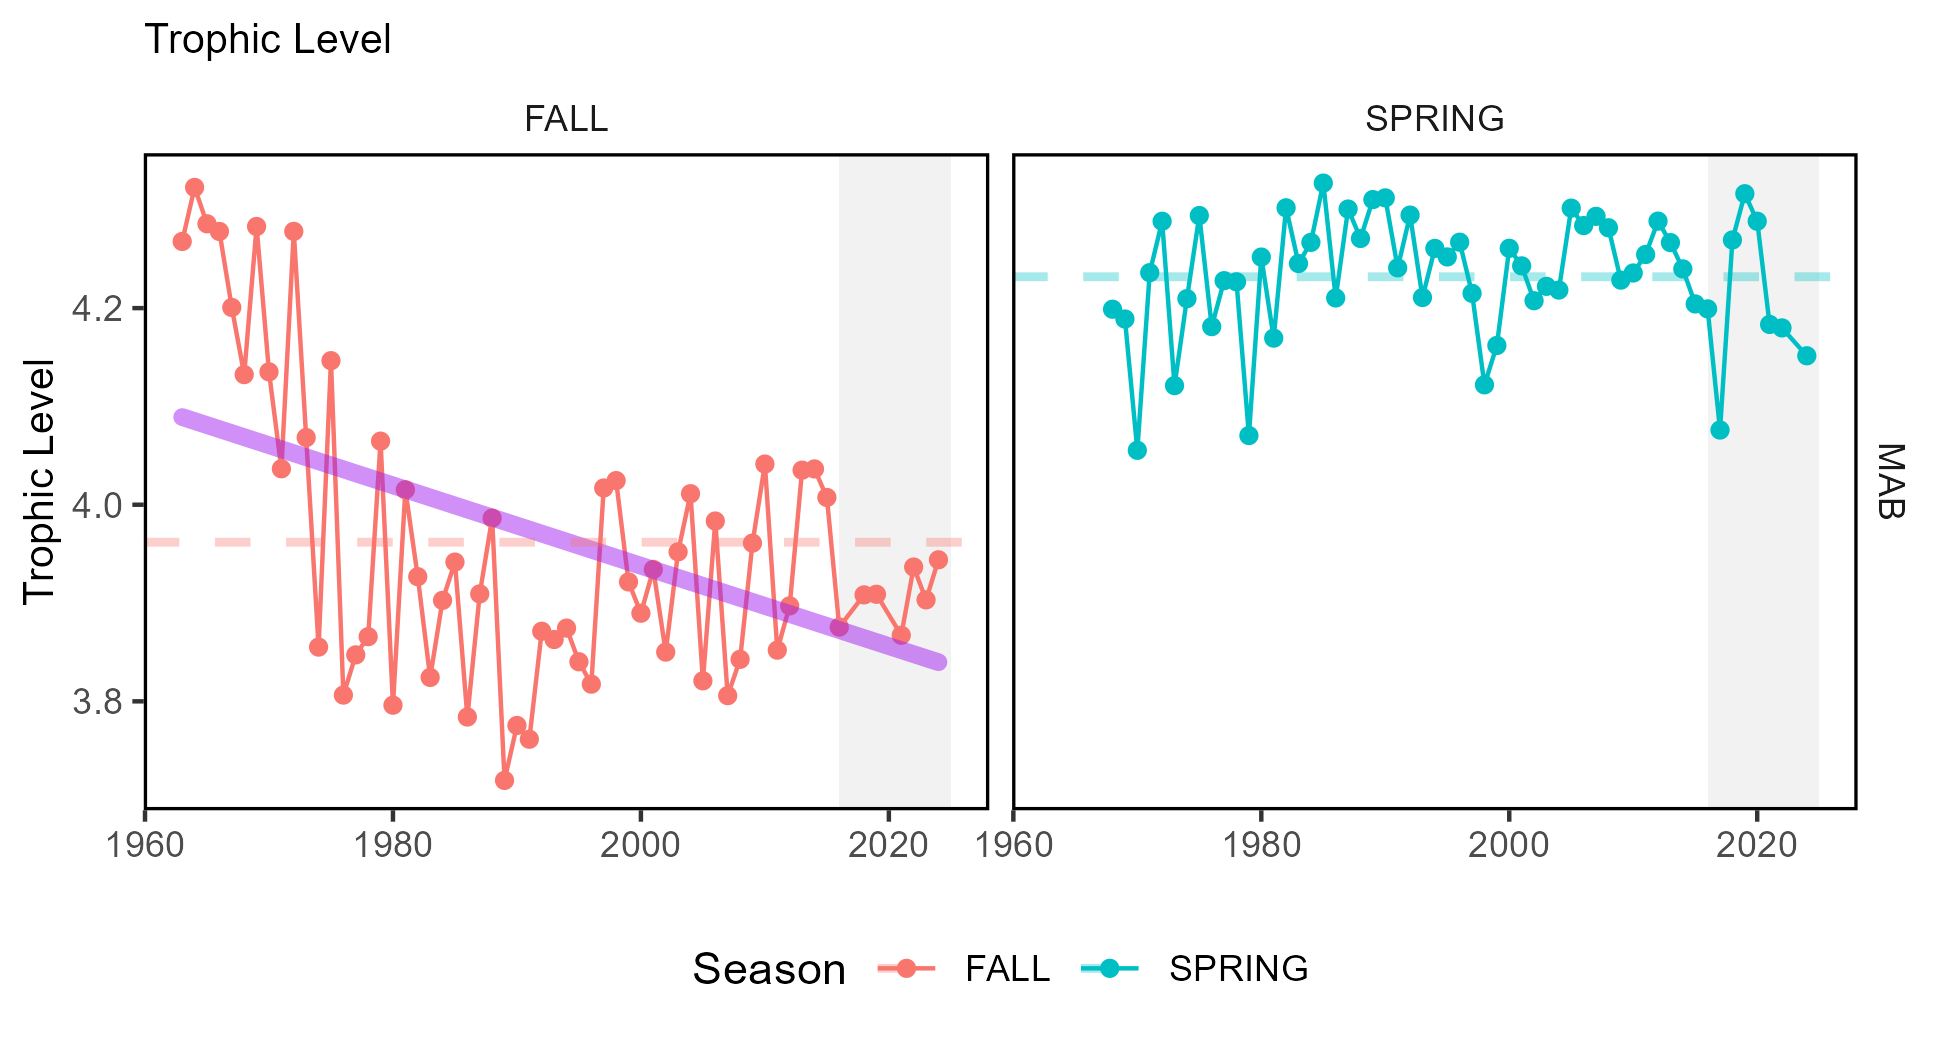
\includegraphics[width=1\linewidth,]{images/MidAtlantic/traits_tl_MidAtlantic_2026-03-27} 

}

\caption{Fish community functional traits (trophic level) in the Mid-Atlantic Bight based on Fall (red) and Spring (blue) survey data with a significant long-term decrease (purple) present in the fall. Dashed lines represent the long-term annual mean for each survey.}\label{fig:traits-tl}
\end{figure}

\subsubsection{Implications}\label{implications-5}

Fleet diversity indices are used by the MAFMC in their EAFM risk assessment to evaluate stability objectives, as well as risks to fishery resilience and maintaining equity in access to fishery resources. Instability in the commercial fleet count metric suggests lower capacity to respond to the current range of fishing opportunities. Commercial species permit revenue diversity is relatively stable (Fig. \ref{fig:commercial-div-species-div}) but comparisons are limited by missing historical (pre-2003) clam fishery data.

Declining recreational fleet effort diversity indicates that the party/charter boat sector continues to contract, with shoreside angling becoming a greater percentage of recreational angler trips. Stability in recreational species catch diversity has been maintained by a different set of species over time. Since the 1990s, there has been an increase in Atlantic States Marine Fisheries Commission (ASMFC) and South Atlantic Fishery Management Council (SAFMC) managed species in recreational catch, concomitant with a decline in MAFMC and New England Fishery Management Council (NEFMC) managed species. These changes in effort and species trends may necessitate new or changing management considerations to ensure effective tools and opportunities are in place to support recreational fisheries.

Production at the base of the food web is variable but stable over time. Mid-Atlantic species composition is changing, shifting towards a higher proportion of benthic and demersal fish. Stable adult fish diversity indicates the same overall number and evenness over time, but doesn't rule out species substitutions (e.g., warm-water species replacing cold-water species). There is evidence for long-term change in finfish trait distributions in the Mid-Atlantic. Future research should consider how changes in single species abundances may influence ecosystem stability.

In the MAB, both the fisheries and ecosystem are exhibiting long-term systemic shifts away from historical norms. While these changes don't appear abrupt like one would expect during a regime shift, they do indicate a potential change in baseline conditions.

\section{Risks to Meeting Fishery Management Objectives}\label{risks-to-meeting-fishery-management-objectives}

\subsection{Climate and Ecosystem Change}\label{climate-and-ecosystem-change}

\subsubsection{Risks to managing spatially}\label{risks-to-managing-spatially}

Shifting species distributions, including changes in spatial extent or center of distribution, alter both species and fishery interactions. In particular, shifting species distributions can affect expected management outcomes when spatial allocations and bycatch measures are based on historical fish and protected species distributions. Species availability to surveys can also change as distributions shift within or outside of survey footprints, complicating the interpretation of survey trends.

Coastwide indicators are reviewed in this section to evaluate spatial change throughout the Northeast US shelf. Indicators are identical between the Mid-Atlantic and New England reports.

\paragraph{Indicators: Fish and protected species distribution shifts}\label{indicators-fish-and-protected-species-distribution-shifts}

As noted in the \hyperref[implications]{Seafood Production Implications section}, the combined center of \href{https://noaa-edab.github.io/catalog/species_dist.html}{distribution} for 48 Northeast Shelf commercially or ecologically important fish species continues to show movement towards the northeast and generally into deeper water (Fig. \ref{fig:species-dist}). An analysis of recreational landings data from 2002 to 2019 found evidence of distribution shifts for several \href{https://noaa-edab.github.io/catalog/species_dist.html}{highly migratory species}, including sharks, billfish and tunas.

\href{https://noaa-edab.github.io/catalog/habitat_diversity.html}{Habitat model-based species richness} suggests shifts of both cooler and warmer water species to the northeast. Similar patterns have been found for \href{https://noaa-edab.github.io/catalog/cetacean_dist.html}{marine mammals}, with multiple species shifting northeast between 2010 and 2017 in most seasons (Fig. \ref{fig:protectedspp-dist-shifts}).

\begin{figure}[T]

{\centering 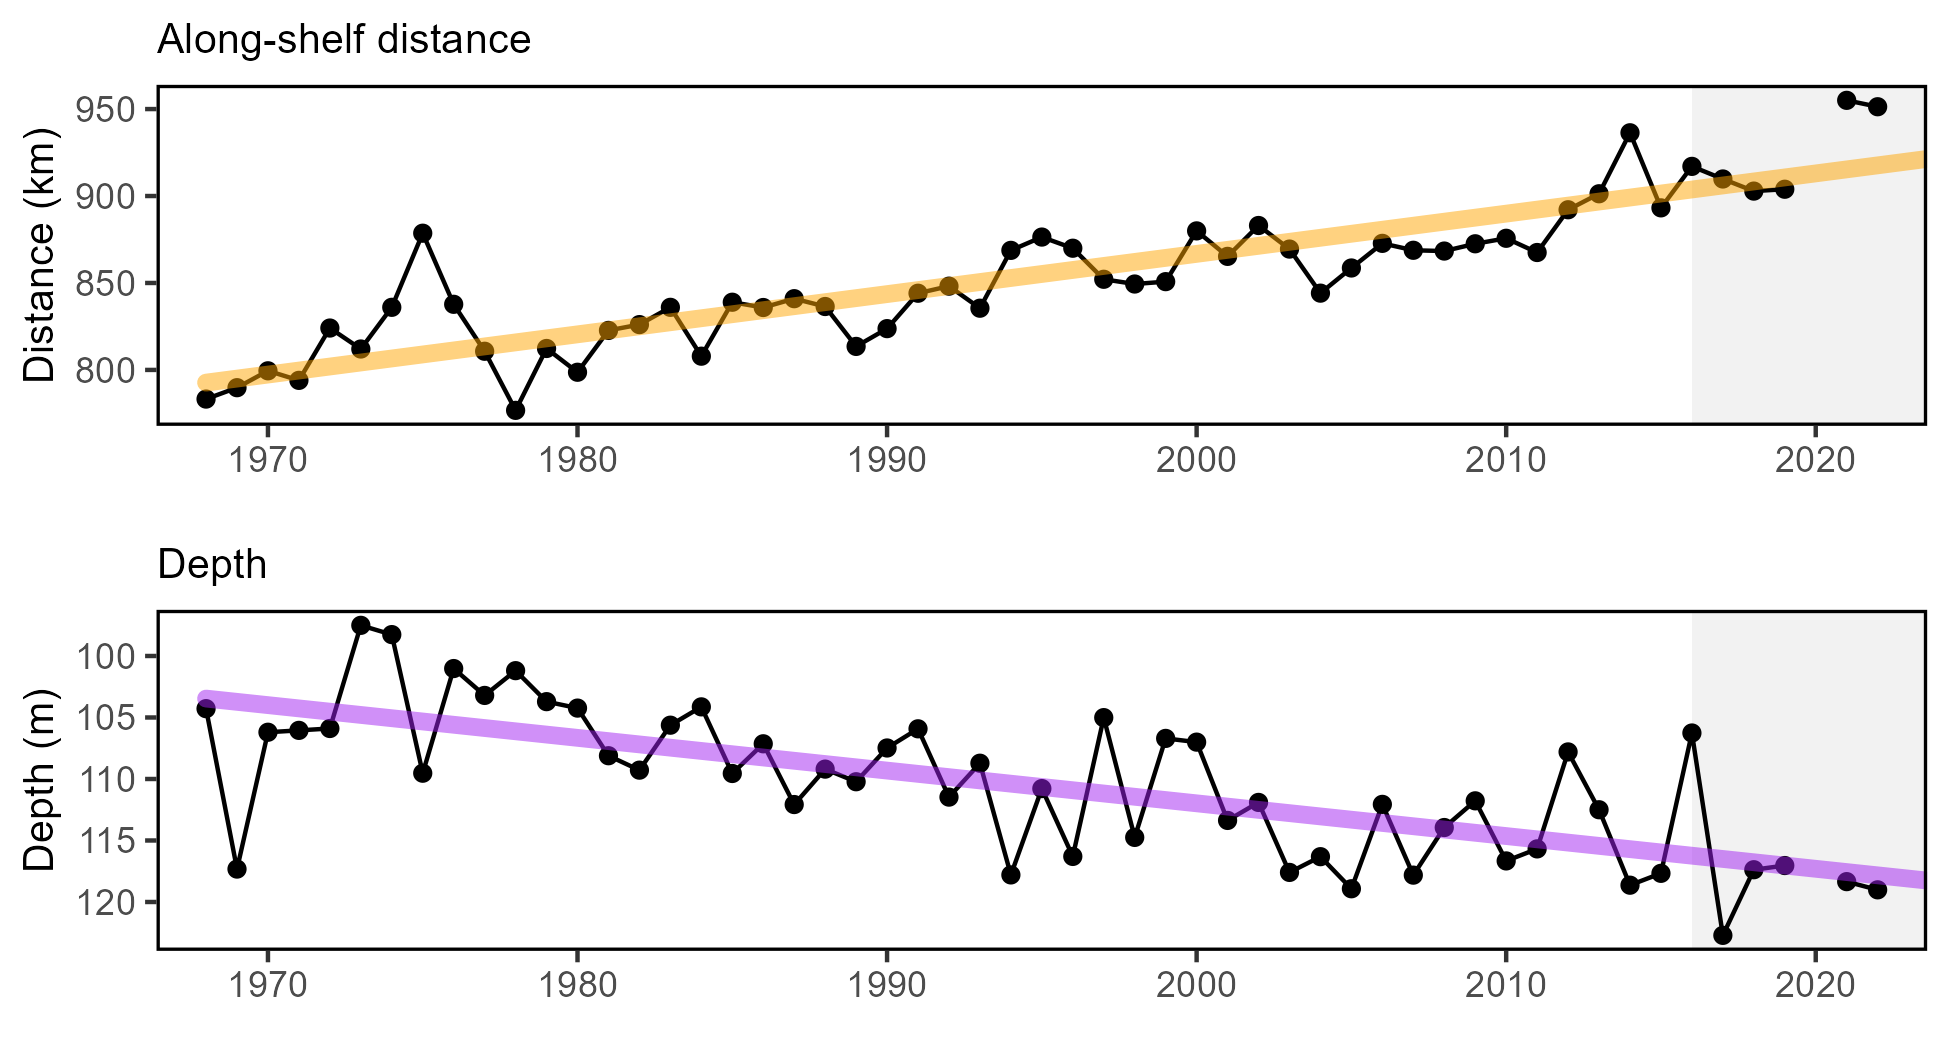
\includegraphics[width=1\linewidth,]{images/BothReports/species_dist_BothReports_2026-03-26} 

}

\caption{Aggregate species distribution metrics for species in the Northeast Large Marine Ecosystem: along shelf distance with long-term increasing trend (orange), and depth with long-term decreasing trend indicating deeper water (purple).}\label{fig:species-dist}
\end{figure}

\begin{figure}[T]

{\centering 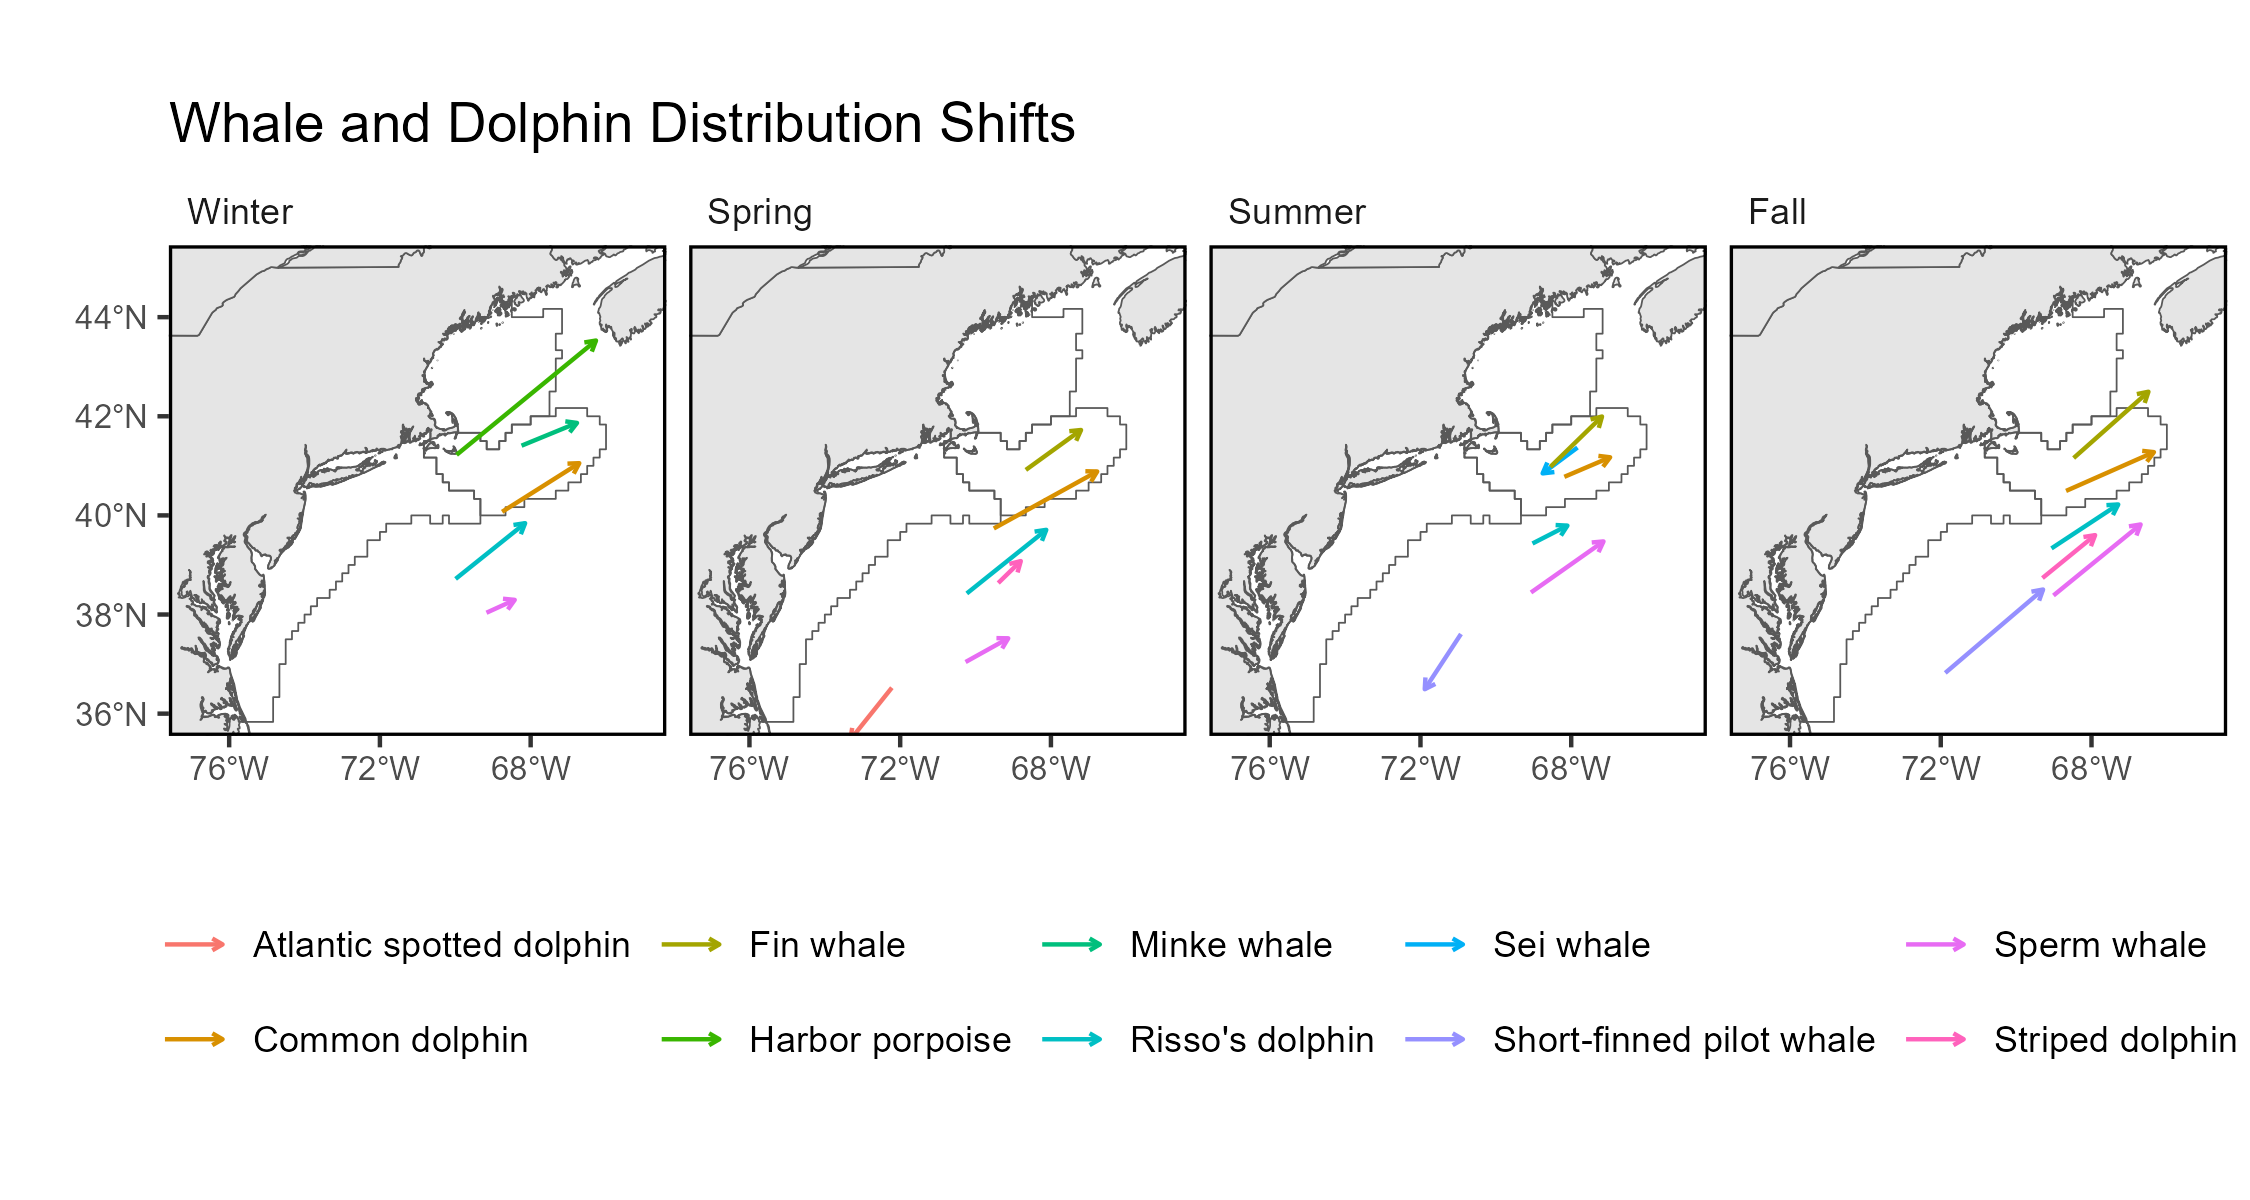
\includegraphics[width=1\linewidth,]{images/BothReports/cetacean_dist_BothReports_2026-03-26} 

}

\caption{Direction and magnitude of core habitat shifts, represented by the length of the line of the seasonal weighted centroid for species with more than 70 km difference between 2010 and 2017 (tip of arrow).}\label{fig:protectedspp-dist-shifts}
\end{figure}

\paragraph{Drivers:}\label{drivers}

Mobile populations shift distributions to maintain suitable habitat and prey fields, possibly expanding ranges if new suitable habitat exists. Changes in managed species distribution is partially related to the \href{https://noaa-edab.github.io/catalog/forage_index.html}{distribution of forage biomass}. Since 1982, the fall center of gravity of forage fish (20 species combined) has moved to the north and east (Fig. \ref{fig:forageshifts}). Spring forage fish center of gravity has moved northward but without an eastward trend. Some of the whale and dolphin distribution shifts (Fig. \ref{fig:protectedspp-dist-shifts}) are likely in response to these forage fish shifts. \href{https://noaa-edab.github.io/catalog/zooplankton_index.html\#key-results-and-visualizations-4}{Small copepods}, widespread prey of many larval and juvenile fish, show a similar shift in center of gravity as forage fish, to the north and east in the fall, as well as northward in spring (Fig. \ref{fig:smallcopeall-cog}.

\begin{figure}[T]

{\centering 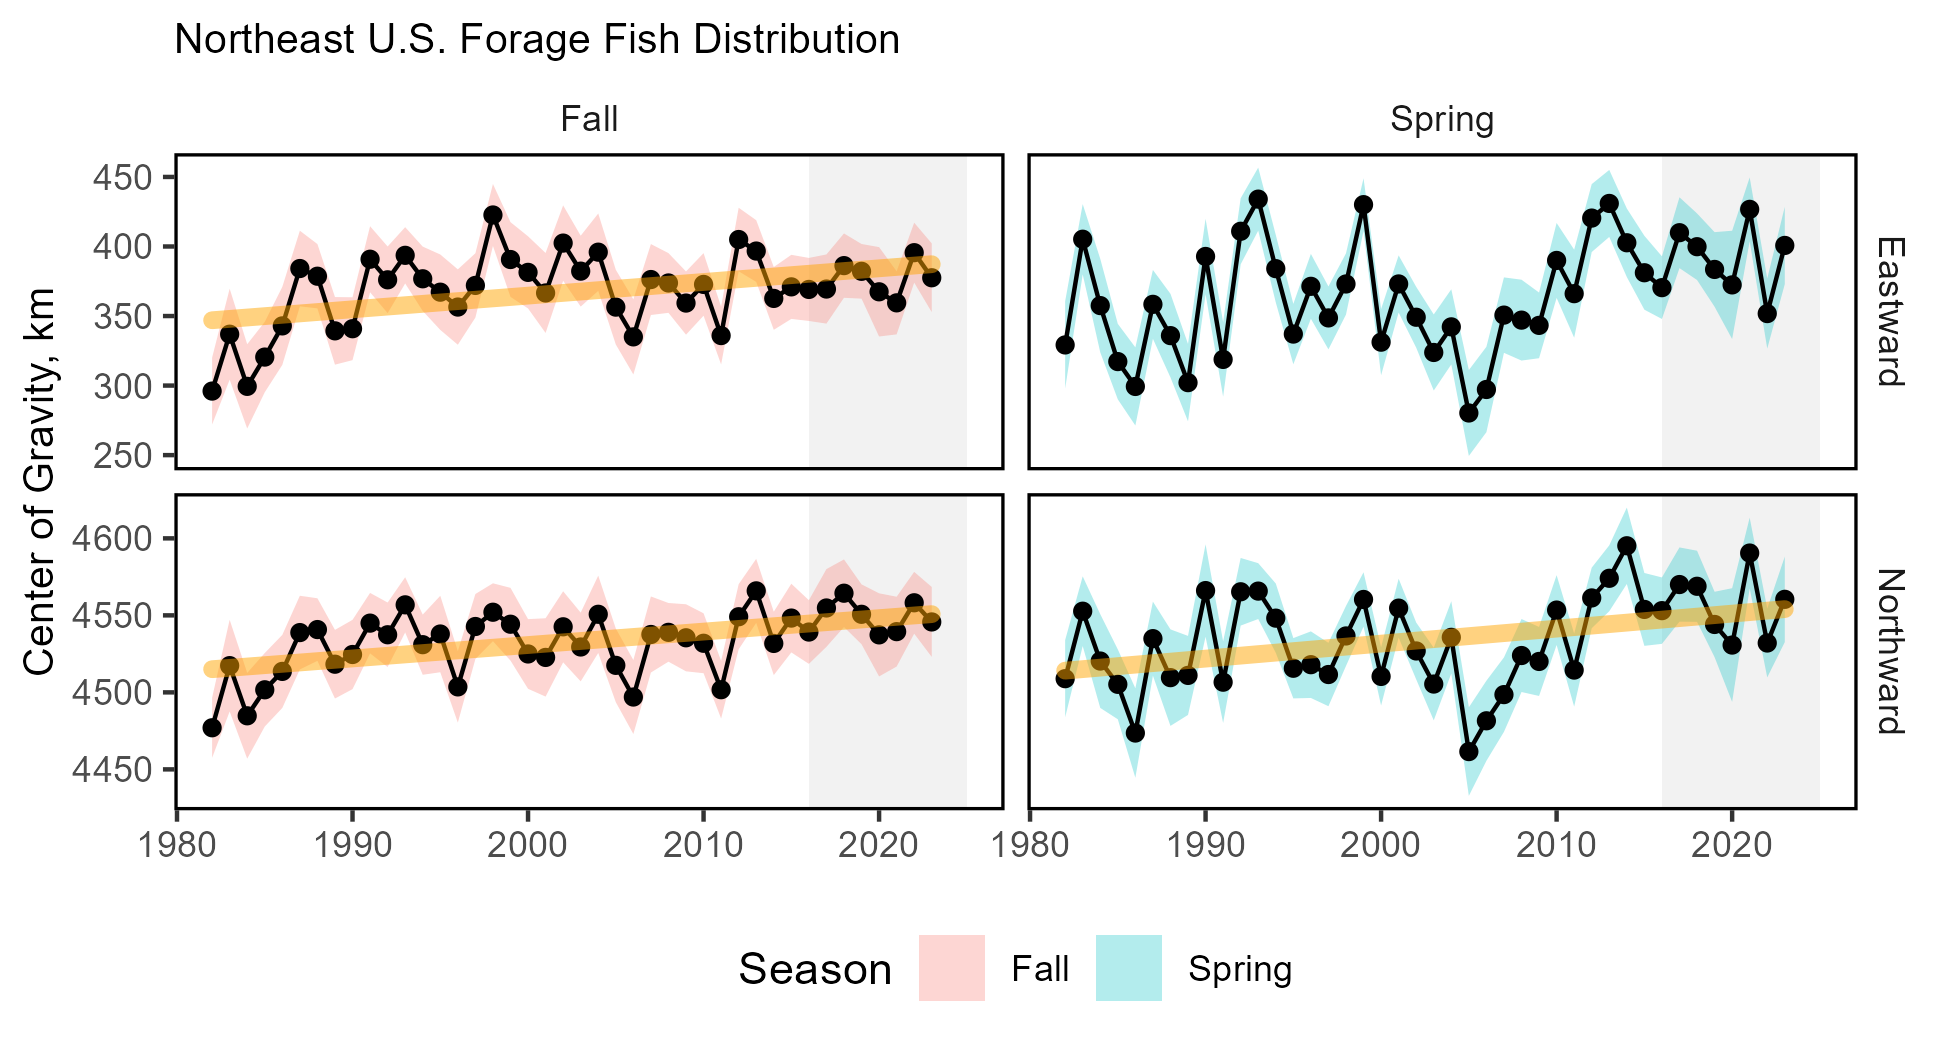
\includegraphics[width=1\linewidth,]{images/BothReports/forage_dist_BothReports_2026-03-27} 

}

\caption{Eastward (top) and northward (bottom) shifts in the center of gravity for 20 forage fish species on the Northeast U.S. Shelf in fall (left) and spring (right), with long-term increasing trends (orange) for fall eastward and northward and spring northward center of gravity.}\label{fig:forageshifts}
\end{figure}

\begin{figure}[T]

{\centering 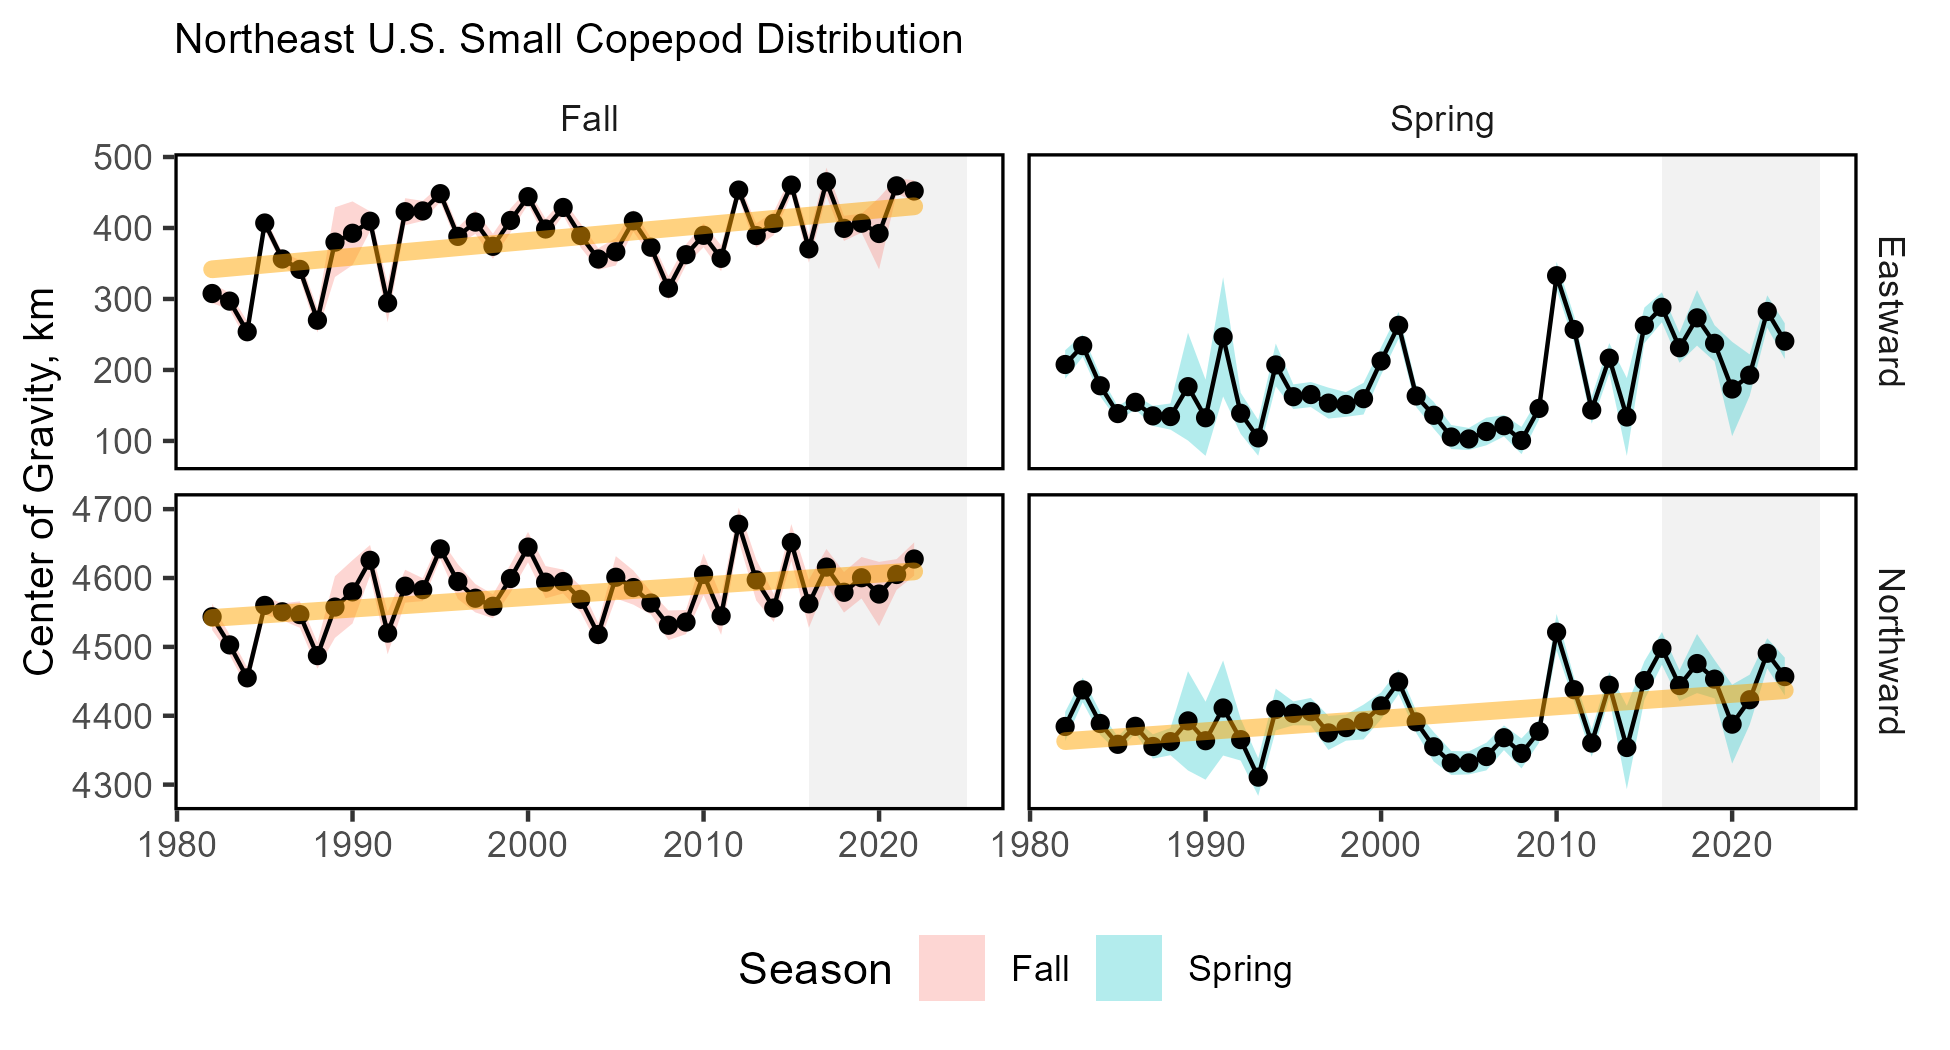
\includegraphics[width=1\linewidth,]{images/BothReports/smallcopeall_cog_BothReports_2026-03-27} 

}

\caption{Eastward (top) and northward (bottom) shifts in the center of gravity for small copepod species on the Northeast U.S. Shelf in fall (left) and spring (right), with long-term increasing trends (orange)  in fall eastward and fall and spring northward center of gravity}\label{fig:smallcopeall-cog}
\end{figure}

Megabenthos center of gravity shows a short-term eastward trend in spring (Fig. \ref{fig:megabenthosshifts}). Megabenthos are large, non-federally-managed benthic invertebrates sampled by scallop dredge, otter trawl, and the Campbell grab. These include crabs, decapods, and sea stars, which are often prey for many managed species.

\begin{figure}[T]

{\centering 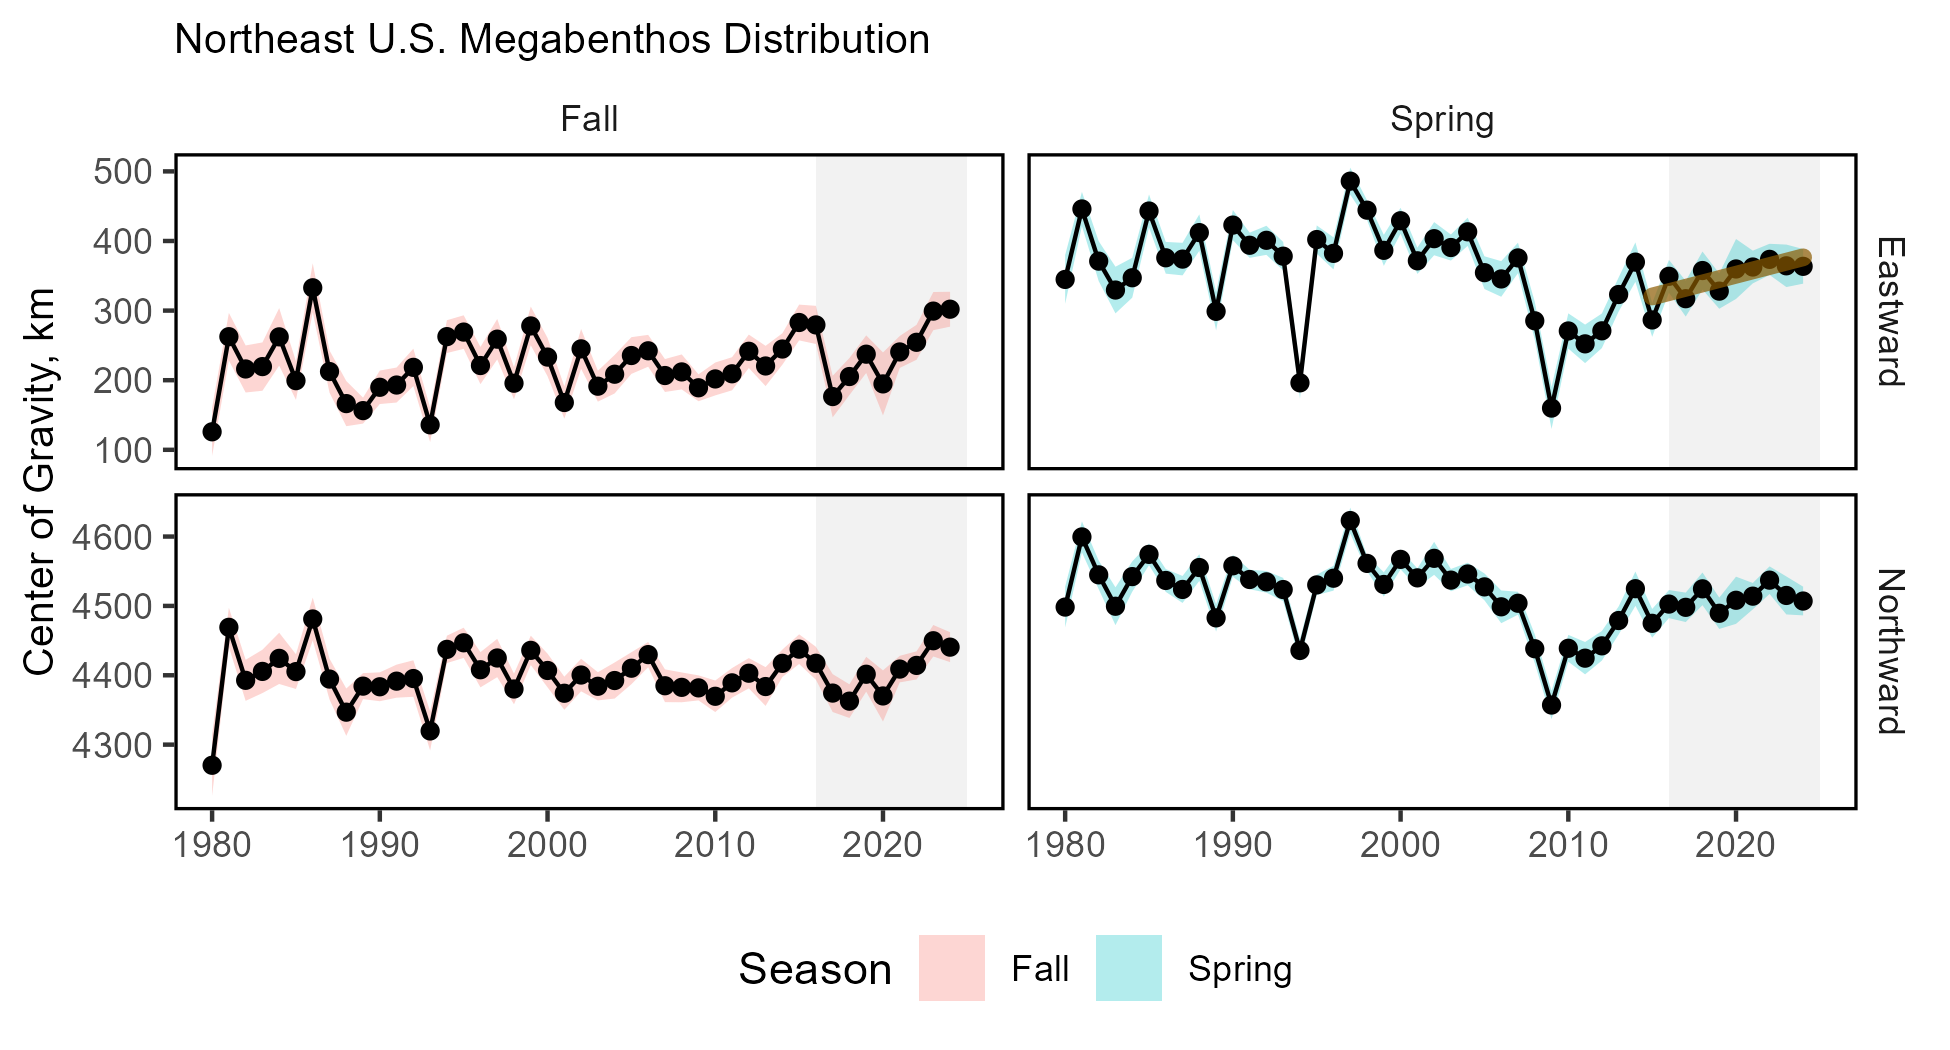
\includegraphics[width=1\linewidth,]{images/BothReports/megabenthos_dist_BothReports_2026-03-27} 

}

\caption{Eastward (top) and northward (bottom) shifts in the center of gravity for megabenthos species on the Northeast U.S. Shelf in fall (left) and spring (right), with short-term increasing trend (orange) for spring eastward center of gravity.}\label{fig:megabenthosshifts}
\end{figure}

In contrast, \href{https://noaa-edab.github.io/catalog/benthos_index.html}{macrobenthos} center of gravity has shifted west and south in the spring (Fig. \ref{fig:macrobenthosshifts}). Macrobenthos are small bottom-dwelling invertebrates including polychaete worms, small crustaceans, bivalves (non-commercial), gastropods, nemerteans, tunicates, cnidarians, brittle stars, sea cucumbers, and sand dollars, and are prey for many managed species.

\href{https://noaa-edab.github.io/catalog/zooplankton_index.html\#key-results-and-visualizations-4}{Large copepods} (including \emph{Calanus finmarchicus}) and euphausiids do not have long-term trends in their centers of gravity (Fig. \ref{fig:lgcopeall-cog}, \ref{fig:euph-cog}). Some targeted species distributions may shift in response to these shifts in forage, copepod, and macrobenthos distributions.

\begin{figure}[T]

{\centering 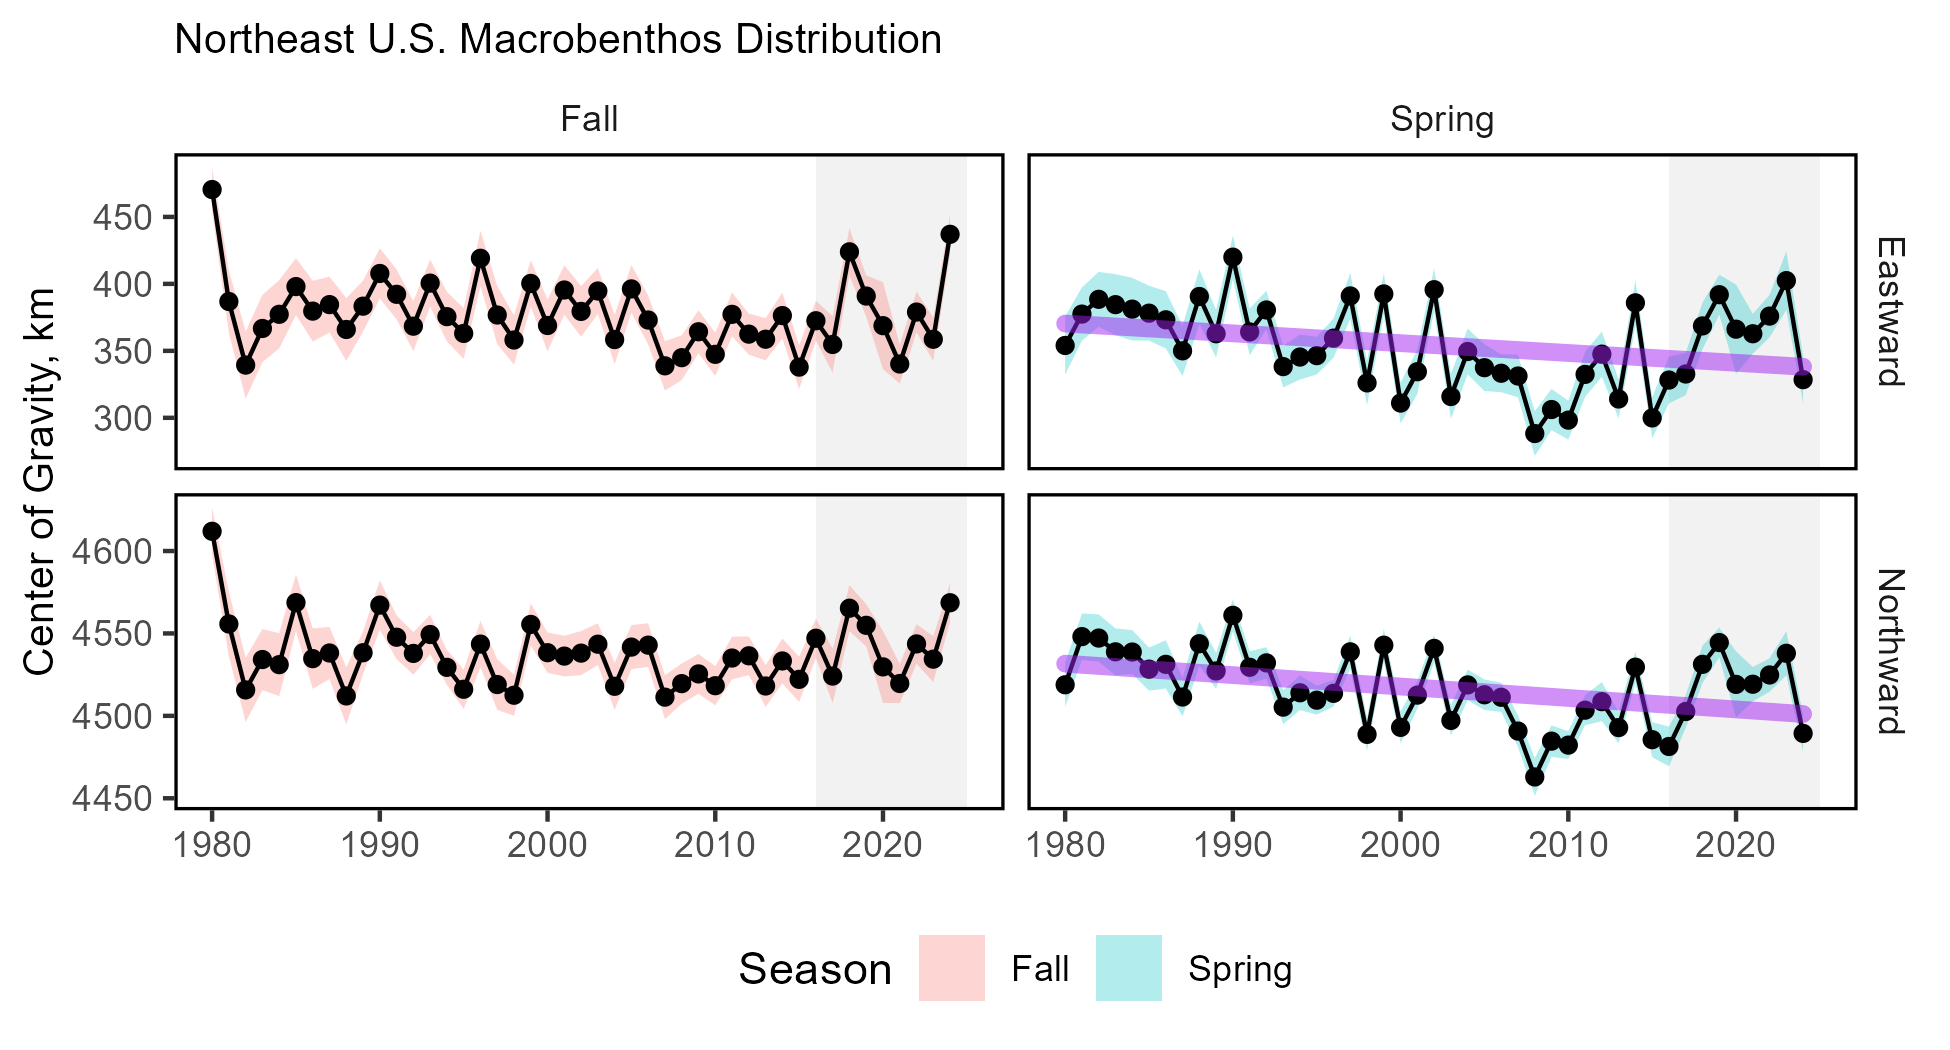
\includegraphics[width=1\linewidth,]{images/BothReports/macrobenthos_dist_BothReports_2026-03-27} 

}

\caption{Eastward (top) and northward (bottom) shifts in the center of gravity for macrobenthos species on the Northeast U.S. Shelf in fall (left) and spring (right), with long-term decreasing trends (purple) for spring eastward and northward center of gravity.}\label{fig:macrobenthosshifts}
\end{figure}

\begin{figure}[T]

{\centering 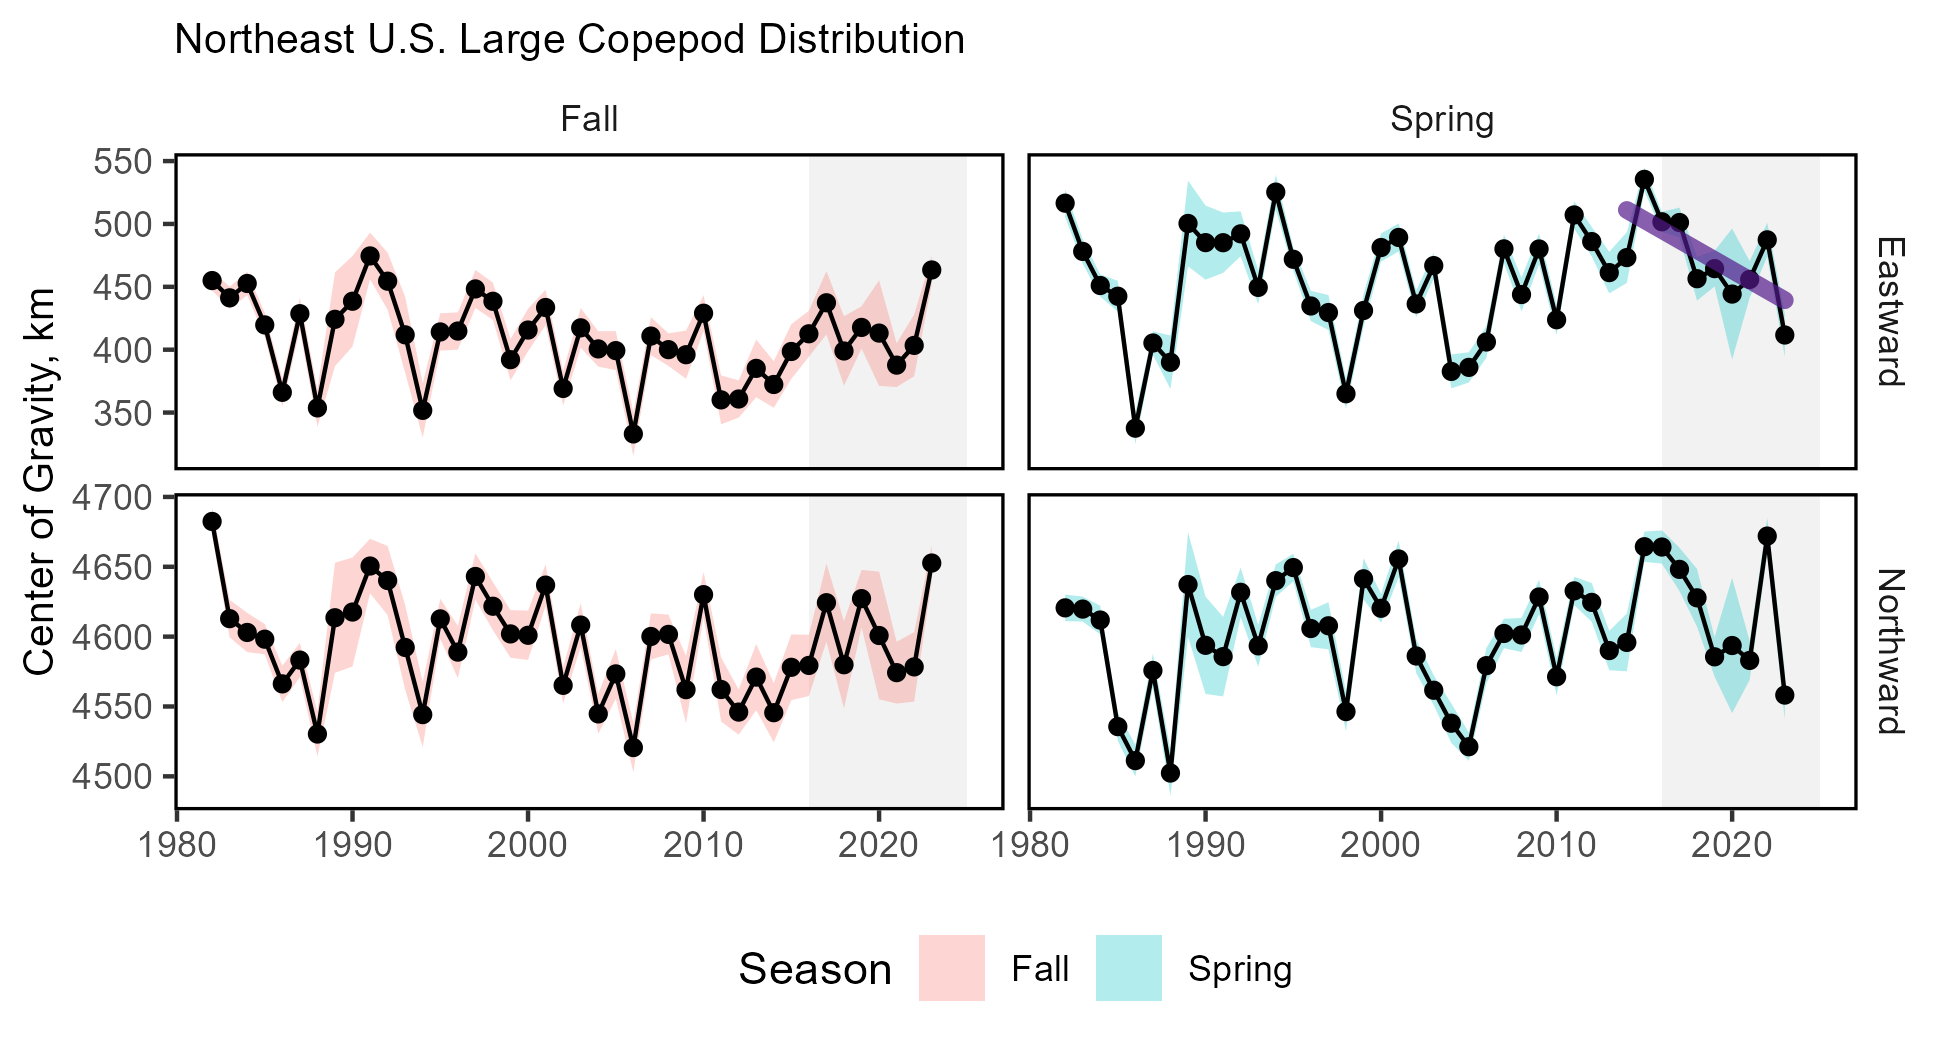
\includegraphics[width=1\linewidth,]{images/BothReports/lgcopeall_cog_BothReports_2026-03-27} 

}

\caption{Eastward (top) and northward (bottom) shifts in the center of gravity for large copepod species (\textit{Calanus finmarchicus}, \textit{Metridia lucens}, \textit{Calanus minor}, \textit{Eucalanus sp.}, \textit{Calanus spp.}) on the Northeast U.S. Shelf in fall (left) and spring (right). }\label{fig:lgcopeall-cog}
\end{figure}

\begin{figure}[T]

{\centering 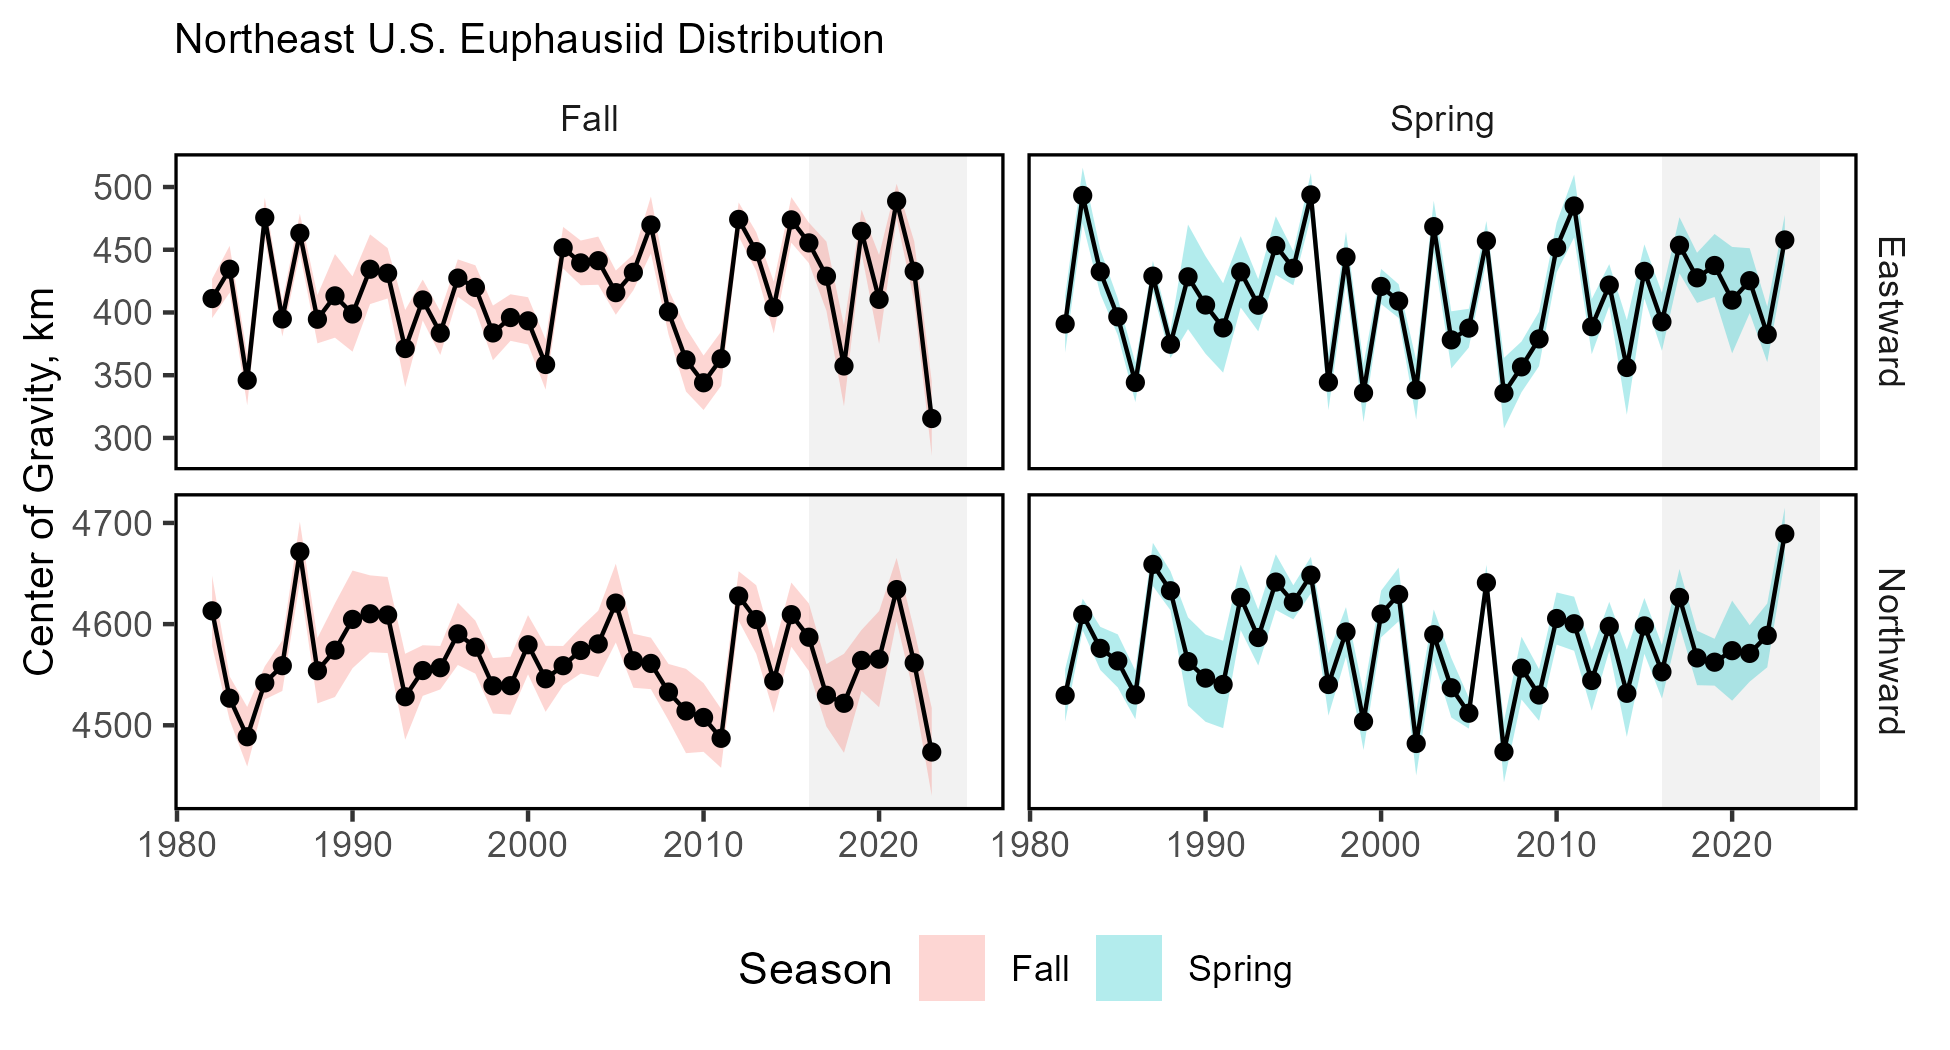
\includegraphics[width=1\linewidth,]{images/BothReports/euph_cog_BothReports_2026-03-27} 

}

\caption{Eastward (top) and northward (bottom) shifts in the center of gravity for Euphausiid species on the Northeast U.S. Shelf in fall (left) and spring (right). }\label{fig:euph-cog}
\end{figure}

Ocean temperatures influence the distribution, seasonal timing, and productivity of managed species (see sections below). The Northeast US shelf, including the Mid-Atlantic, has experienced a continued warming trend for both the \href{https://noaa-edab.github.io/catalog/long_term_sst.html}{long term annual sea surface} (Fig. \ref{fig:long-term-sst}) and \href{https://noaa-edab.github.io/catalog/seasonal_oisst_anom.html}{seasonal surface} (Fig. \ref{fig:seasonal-oisst-anom}) and \href{https://noaa-edab.github.io/catalog/bottom_temp_model_anom.html}{bottom temperature} (Fig. \ref{fig:bottom-temp-anom}, ef\{fig:bottom-temp-insitu\}). However, 2025 surface and bottom temperatures were near normal to cooler than normal conditions in most seasons in the MAB (see also the \hyperref[highlights]{2025 Highlights section}). In 2025, surface temperatures in the MAB were cooler than average in winter and fall, and slightly warmer than average in spring and summer (Fig. \ref{fig:seasonal-oisst-anom}). Bottom temperatures in the MAB were cooler than average or near average in winter, spring, and summer, and warmer than average in fall (Fig. \ref{fig:bottom-temp-anom}). In situ bottom temperature was above average (Fig. ef\{fig:bottom-temp-insitu\}).

\begin{figure}[T]

{\centering 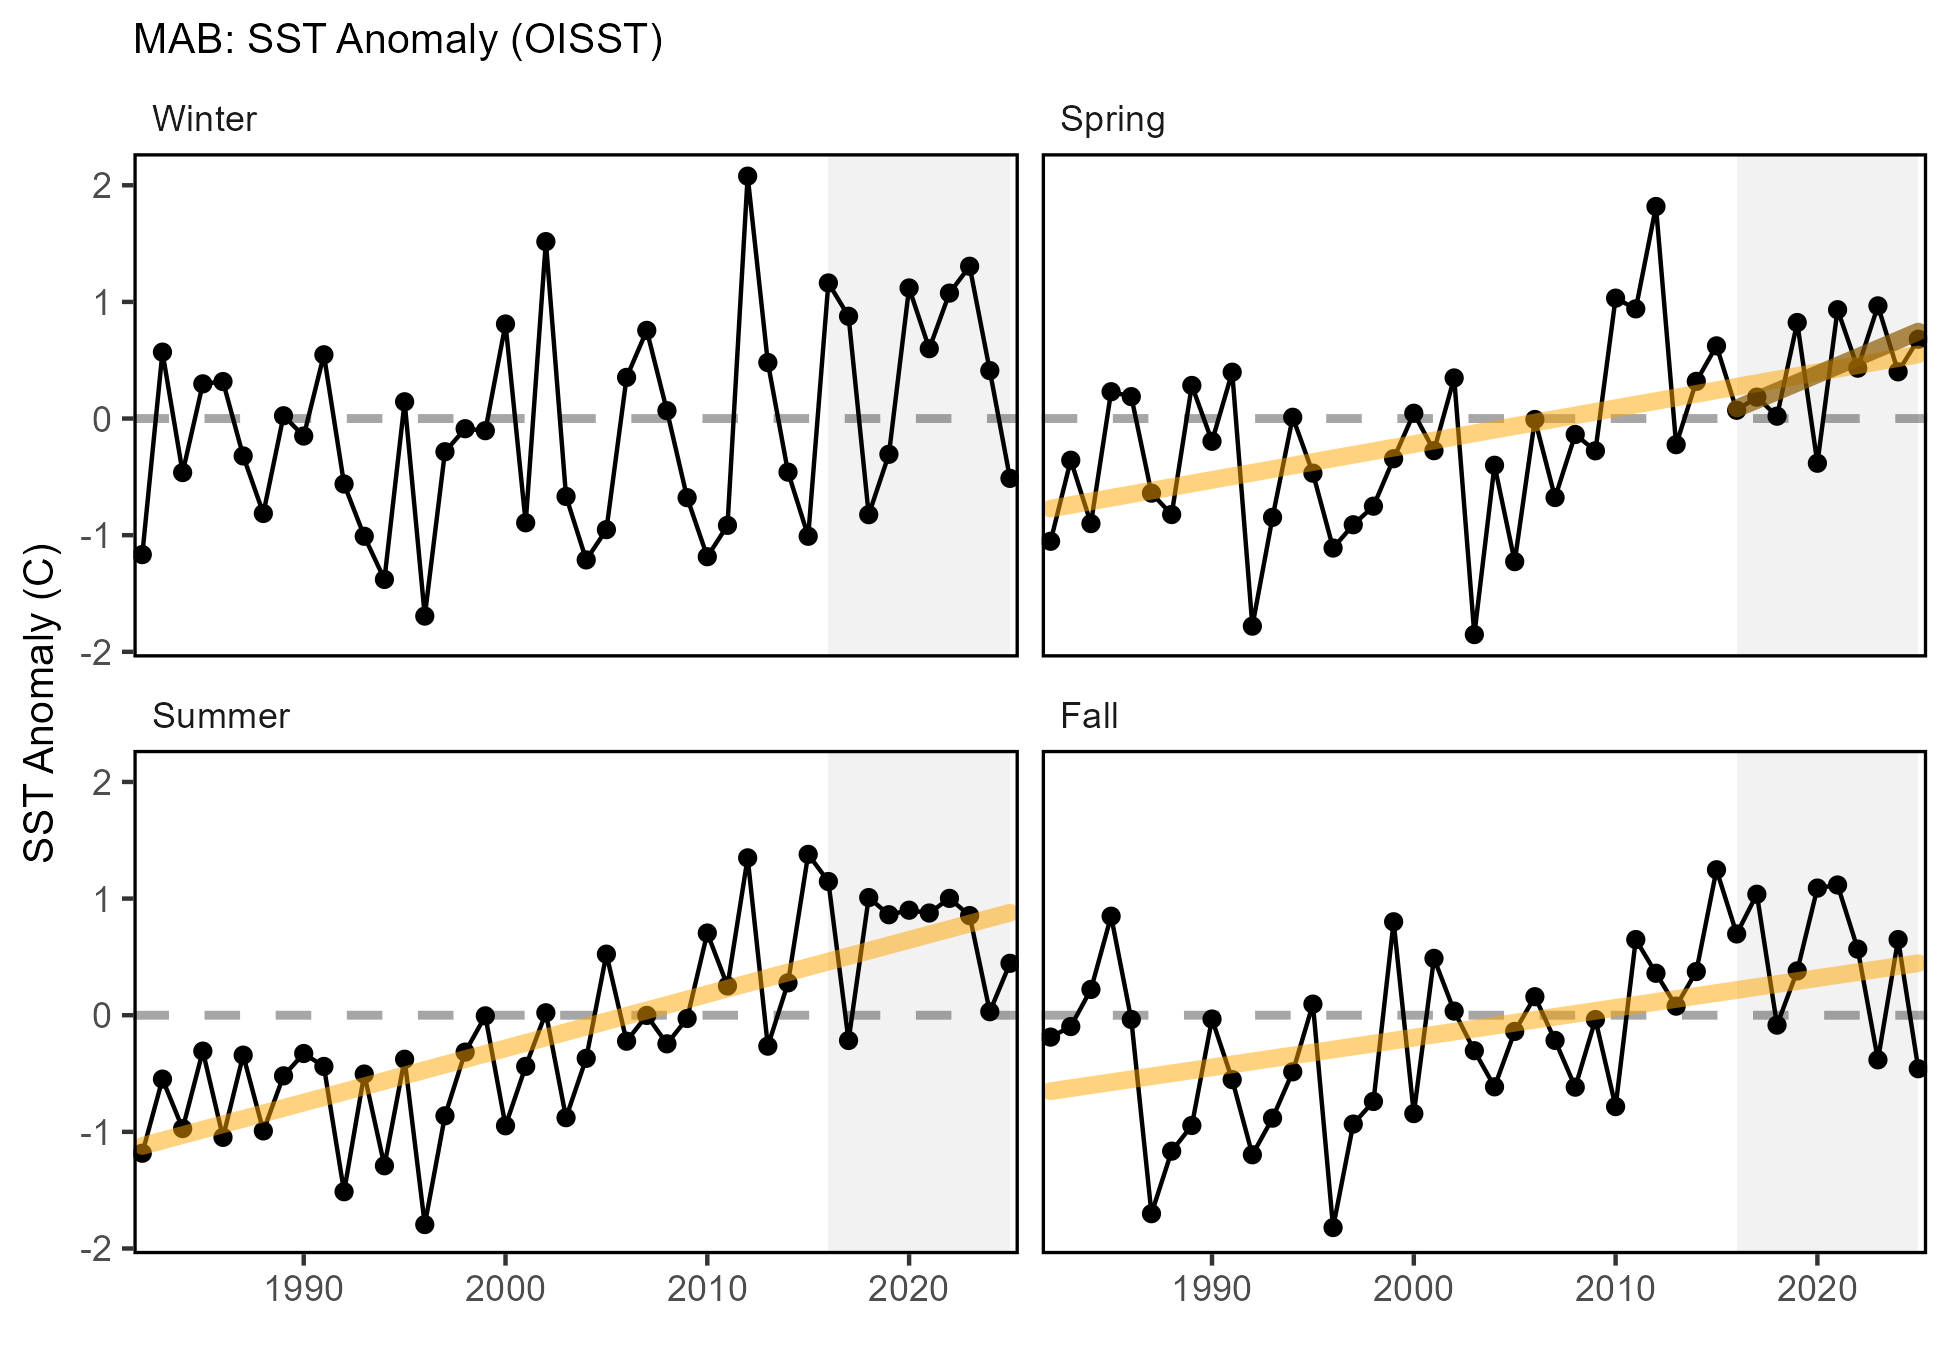
\includegraphics[width=1\linewidth,]{images/MidAtlantic/seasonal_oisst_anom_MidAtlantic_2026-03-26} 

}

\caption{Seasonal Optimum Interpolation Sea Surface Temperature (OISST) anomaly by season for the Mid-Atlantic Bight, with long-term increasing trends (orange) in spring, summer, and fall, and short-term increasing trend in spring.}\label{fig:seasonal-oisst-anom}
\end{figure}

\begin{figure}[T]

{\centering 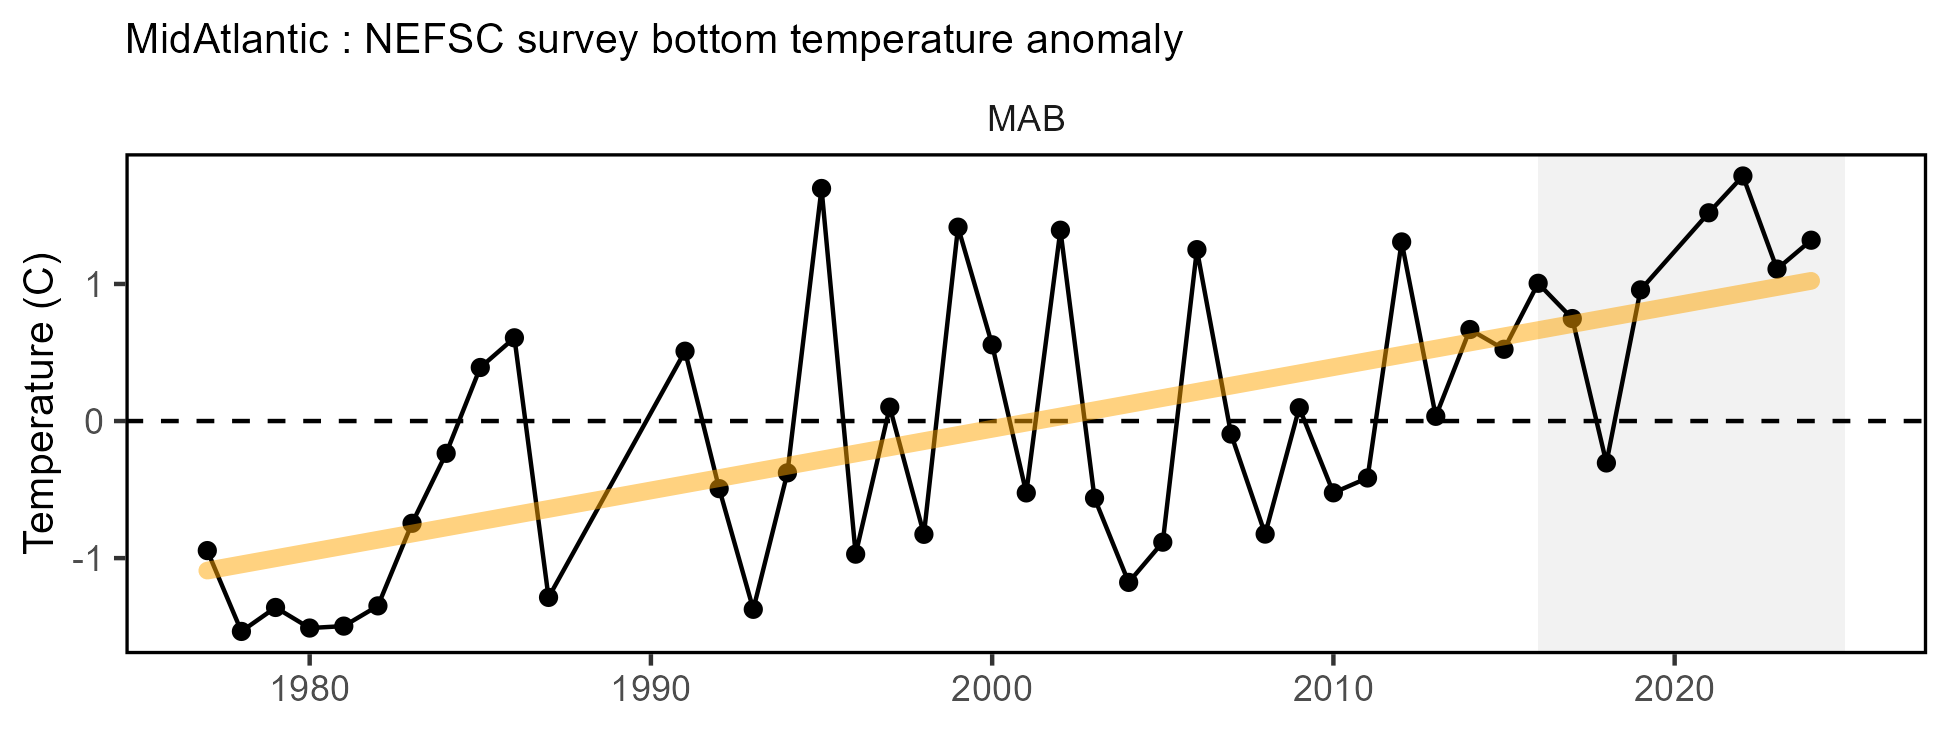
\includegraphics[width=1\linewidth,]{images/MidAtlantic/bottom_temp_insitu_MidAtlantic_2026-03-26} 

}

\caption{Annual in situ bottom temperature anomaly in the Mid-Atlantic, with long-term increasing trends (orange).}\label{fig:bottom-temp-insitu}
\end{figure}

\begin{figure}[T]

{\centering 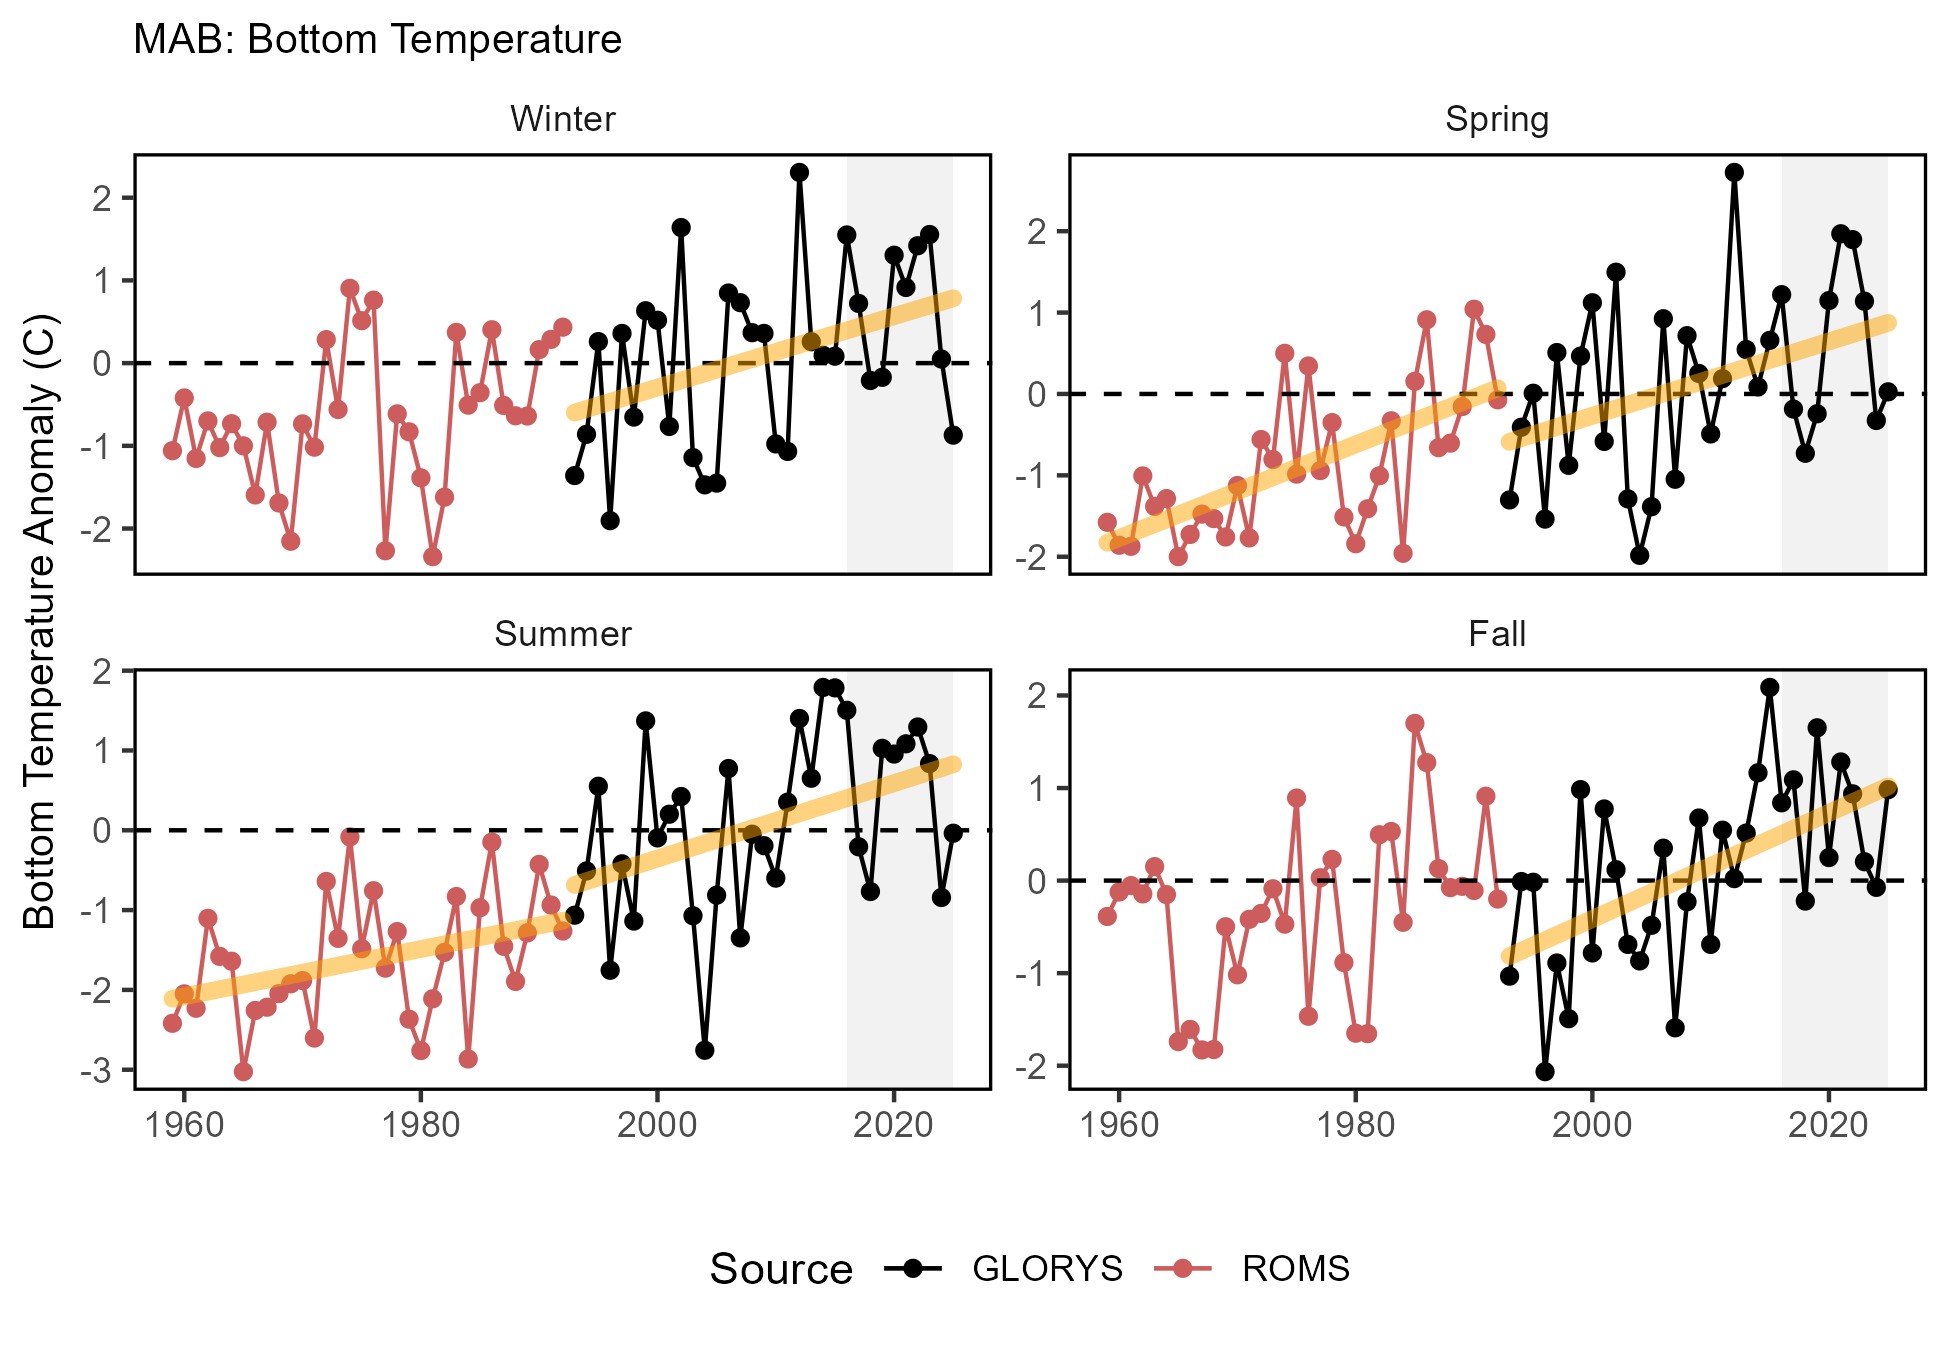
\includegraphics[width=1\linewidth,]{images/MidAtlantic/bottom_temp_anom_MidAtlantic_2026-03-26} 

}

\caption{GLORYS (black) and debiased Regional Ocean Modeling System (ROMS) (red) seasonal bottom temperature anomaly in the Mid-Atlantic Bight, with long-term increasing trends (orange).}\label{fig:bottom-temp-anom}
\end{figure}

Species suitable habitat can expand or contract when changes in temperature and major oceanographic conditions alter distinct water mass habitats. The variability of the Gulf Stream is a major driver of the predominant oceanographic conditions of the Northeast U.S. continental shelf.

The \href{https://noaa-edab.github.io/catalog/gsi.html}{Gulf Stream} has been shifted north of its long-term mean position over much of the last decade (Fig. \ref{fig:GSI}). However, since 2023 the Gulf Stream has shifted southward and remained close to its mean position. With this shift, the supply of Labrador Slope Water has increased along the Northwest Atlantic Shelf. These changes are linked to the cooler water temperatures observed in 2024 and 2025 and shifts in the composition of source waters entering the Gulf of Maine through the Northeast Channel (see \hyperref[highlights]{2025 Highlights}).

\begin{figure}[T]

{\centering 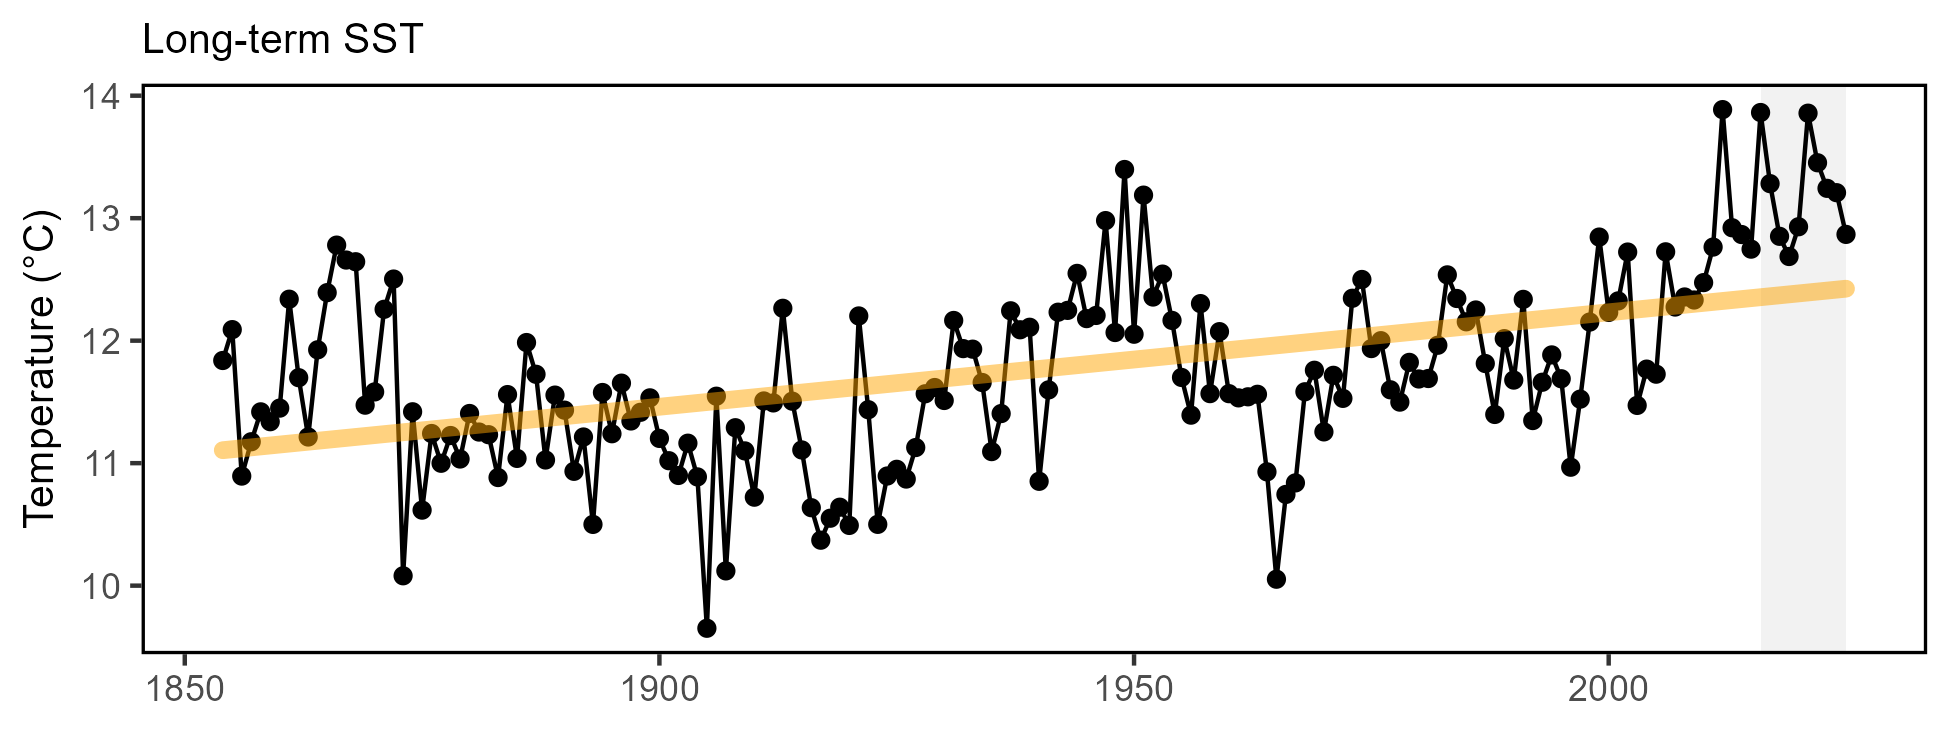
\includegraphics[width=1\linewidth,]{images/BothReports/long_term_sst_BothReports_2026-03-26} 

}

\caption{Northeast U.S. annual sea surface temperature (SST, black), with long-term increasing trend (orange).}\label{fig:long-term-sst}
\end{figure}

\begin{figure}[T]

{\centering 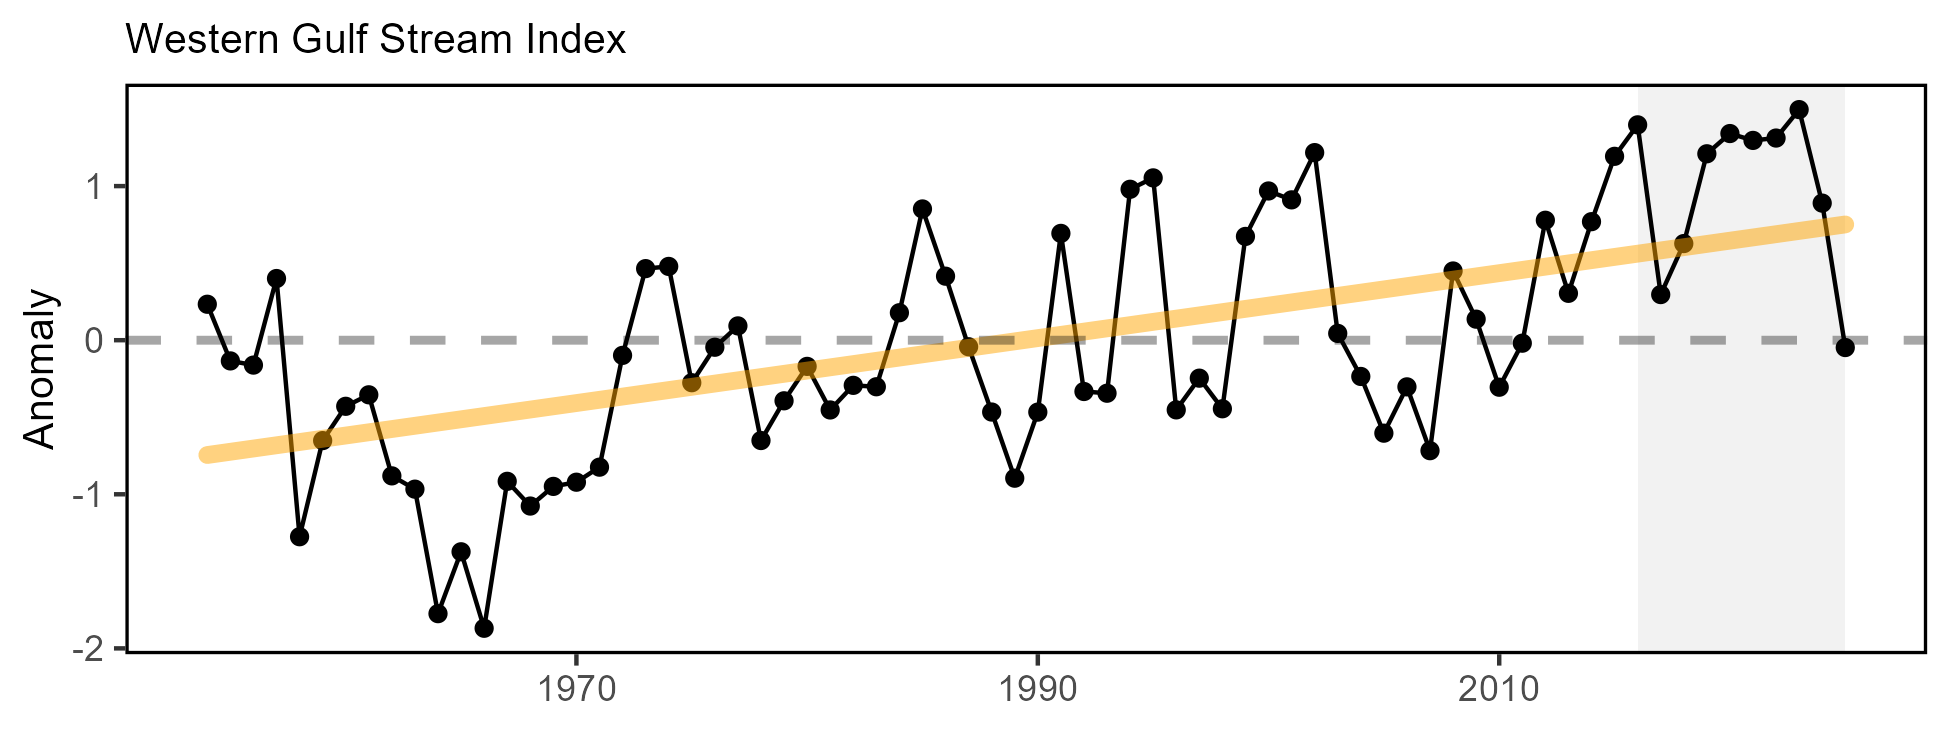
\includegraphics[width=1\linewidth,]{images/BothReports/west_gsi_BothReports_2026-03-26} 

}

\caption{Index representing changes in the location of the western (between 64 and 55 degrees W) Gulf Stream north wall (black). Positive values represent a more northerly Gulf Stream position, with long-term increasing trend (orange).}\label{fig:GSI}
\end{figure}

Changes in ocean temperature and circulation alter habitat features such as the Mid-Atlantic Bight \href{https://noaa-edab.github.io/catalog/cold_pool.html}{Cold Pool}, a band of relatively cold near-bottom water present from spring to fall over the northern MAB. The Cold Pool represents essential fish spawning and nursery habitat, and affects fish distribution and behavior. The Cold Pool has been getting warmer and its areal extent has been shrinking over time (Fig. \ref{fig:cold-pool-size}). In 2025, however, the Cold Pool temperature and extent were above the long-term average, likely due to the influx of Labrador Slope and Scotian Shelf waters into the system. Mobile target species that track a preferred temperature range can show increased interannual variability in their distributions as regional temperatures fluctuate over short periods of time.

\begin{figure}[T]

{\centering 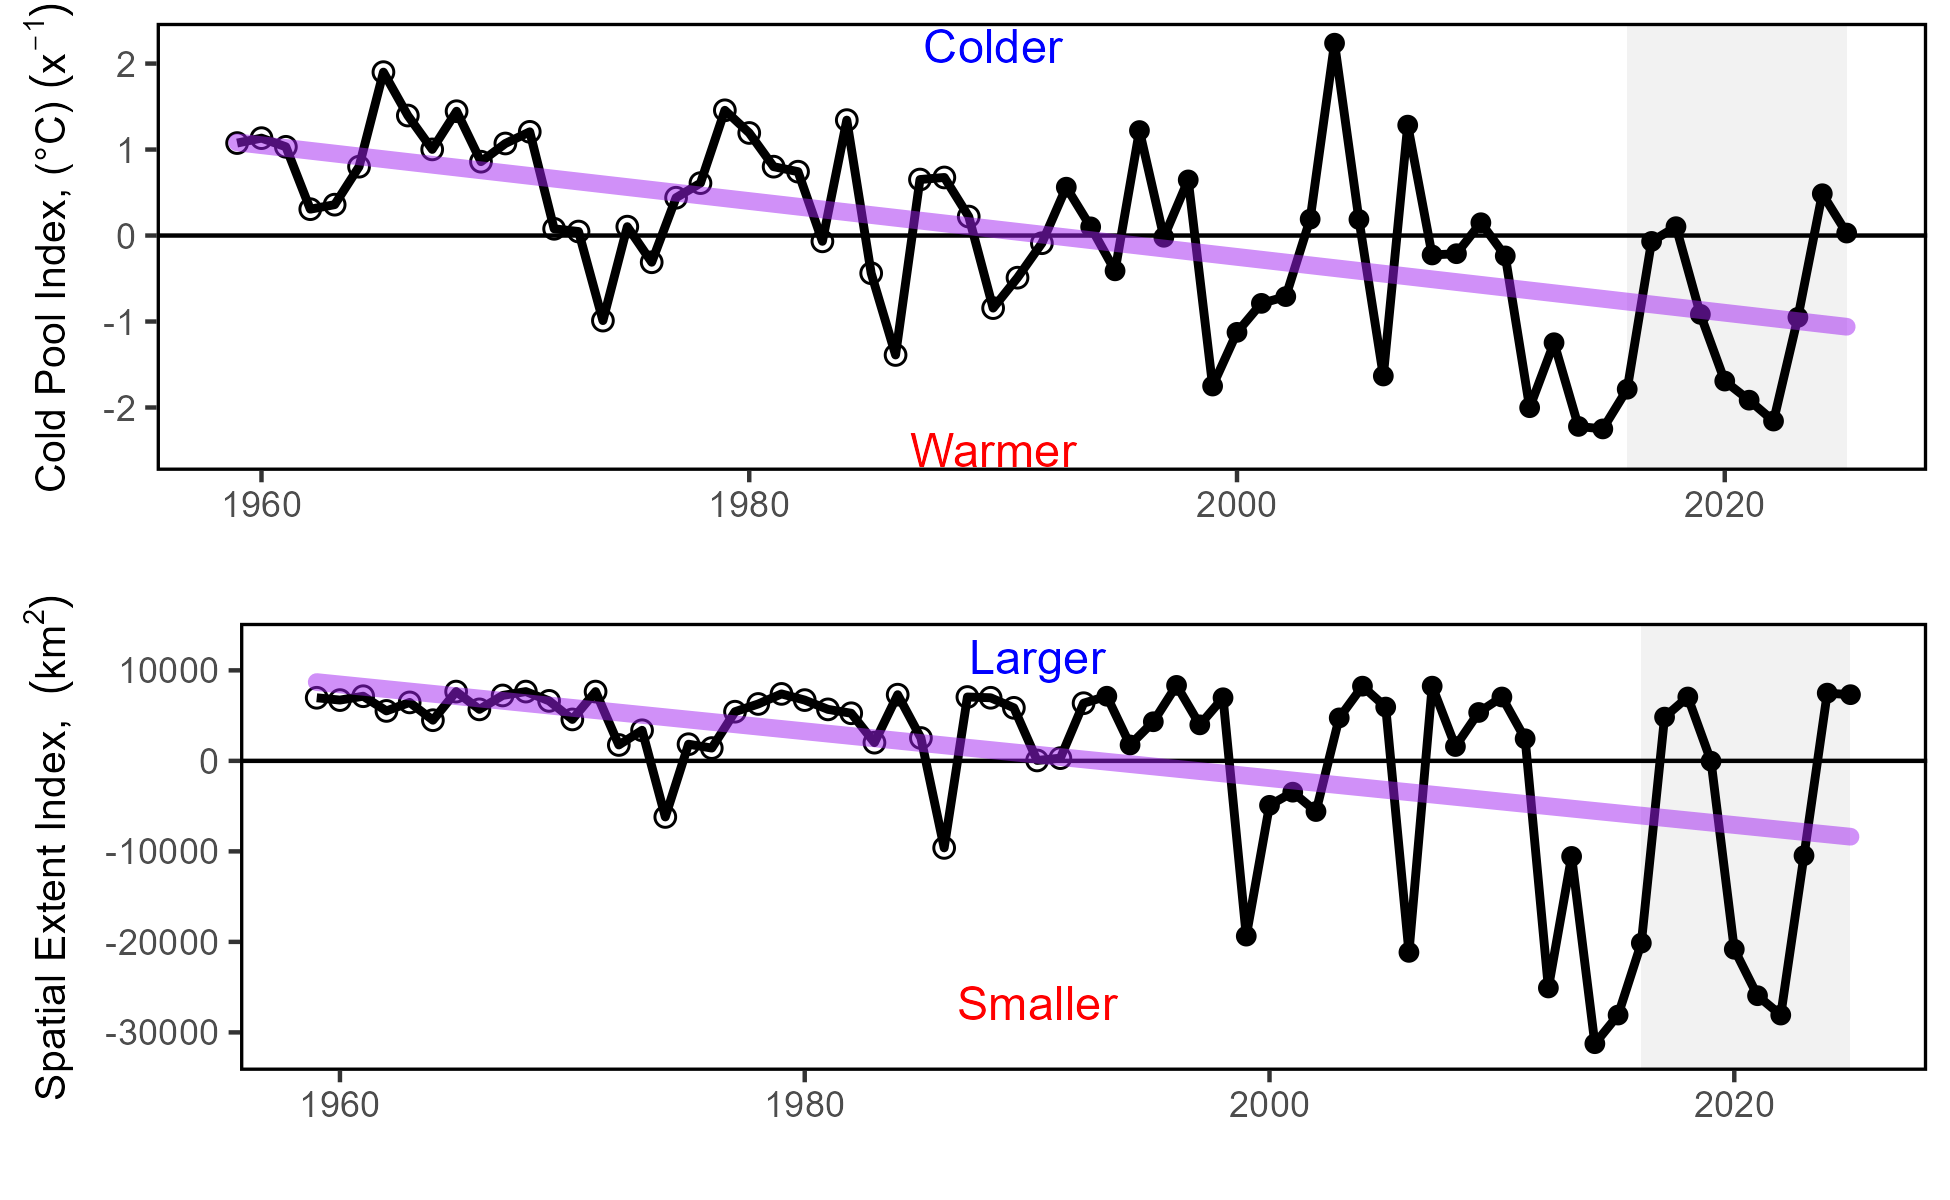
\includegraphics[width=1\linewidth,]{images/BothReports/cold_pool_BothReports_2026-03-18} 

}

\caption{Seasonal cold pool mean temperature (top) and spatial extent index (bottom), based on bias-corrected Regional Ocean Modeling System-Northwest Atlantic (ROMS-NWA) (open circles) and GLORYS (closed circles), with long-term declining trends (purple).}\label{fig:cold-pool-size}
\end{figure}

\paragraph{Future Considerations}\label{future-considerations}

Distribution shifts caused by changes in thermal habitat and ocean circulation are likely to continue as long as long-term trends persist. Episodic and short-term events (see \href{https://noaa-edab.github.io/catalog/observation_synthesis_2024.html}{2024 Highlights} and \hyperref[highlights]{2025 Highlights}) may increase variability in the trends, however species distributions are unlikely to reverse to historical ranges in the short term. Increased mechanistic understanding of distribution drivers is needed to better understand future distribution shifts: species with high mobility or short lifespans react differently from immobile or long-lived species.

\href{https://noaa-edab.github.io/catalog/MOM6_forecasts.html}{MOM6 decadal oceanographic forecasts} suggest a tendency towards near-normal temperatures over the next decade due to decadal variability in regional circulation. 2026 seasonal forecasts show a high probability of below average surface and bottom temperatures in the winter months. Forecast uncertainty is higher during the spring and summer seasons, and above average conditions are predicted for the fall. These forecasts will continue to be evaluated to determine how well they are able to predict episodic and anomalous events that are outside of the long-term patterns.

Adapting management to changing stock distributions and dynamic ocean processes will require continued monitoring of populations in space and time while evaluating management measures against a range of possible future spatial distributions. The upcoming Climate Vulnerability Assessment 2.0 will also be incorporating MOM6 output and forecasts to help predict changes in species distributions and quantify species exposure to predicted future change. Processes like the \href{https://www.mafmc.org/e3cg}{East Coast Coordination Group} and the HMS Climate Vulnerability Assessment can help coordinate management.

\subsubsection{Risks to managing seasonally}\label{risks-to-managing-seasonally}

The effectiveness of seasonal management actions (fishing seasons or area opening/closing periods) depends on a proper alignment with the seasonal life cycle events (phenology) of fish stocks (e.g., migration and spawning timing). If not accounted for, changes in the timing of these biological cycles can reduce the effectiveness of seasonal management measures. The timing of seasonal patterns can also change the interactions between fisheries and non-target species thus influencing bycatch and the availability of species to surveys.

\paragraph{Indicators: Timing shifts}\label{indicators-timing-shifts}

Indicators of phenological changes in fish populations require regular sampling and observations, and therefore a limited number of these indicators are currently available. One indicator shows shifts in \href{https://noaa-edab.github.io/catalog/spawn_timing.html}{spawning timing} of haddock and yellowtail flounder. Spawning of both haddock stocks occurred earlier in the year, as indicated by more resting (post-spawning) stage fish in recent years compared to earlier in the time series (Fig. \ref{fig:spawntiming}). The high percentage of northern stock (Cape Cod/GOM) yellowtail flounder females in the resting maturity stage shown earlier in the time series is reflective of spring surveys sampling them well before spawning, which peaked in June for the northern stock (Fig. \ref{fig:spawntiming}). More recently, the females are much closer to spawning, indicating that yellowtail flounder are spawning earlier in the year. Similarly, increased catch of post-spawning fish in Southern New England indicates that the peak spawning of the southern stock could have also shifted to earlier in the year. Yellowtail flounder spawning is related to bottom temperature, week of year, and decade sampled for each of the three stocks. Changes to spawning times could impact the survival of early life stages of fish, subsequently affecting the population size, health, and market value.

\begin{figure}[T]

{\centering 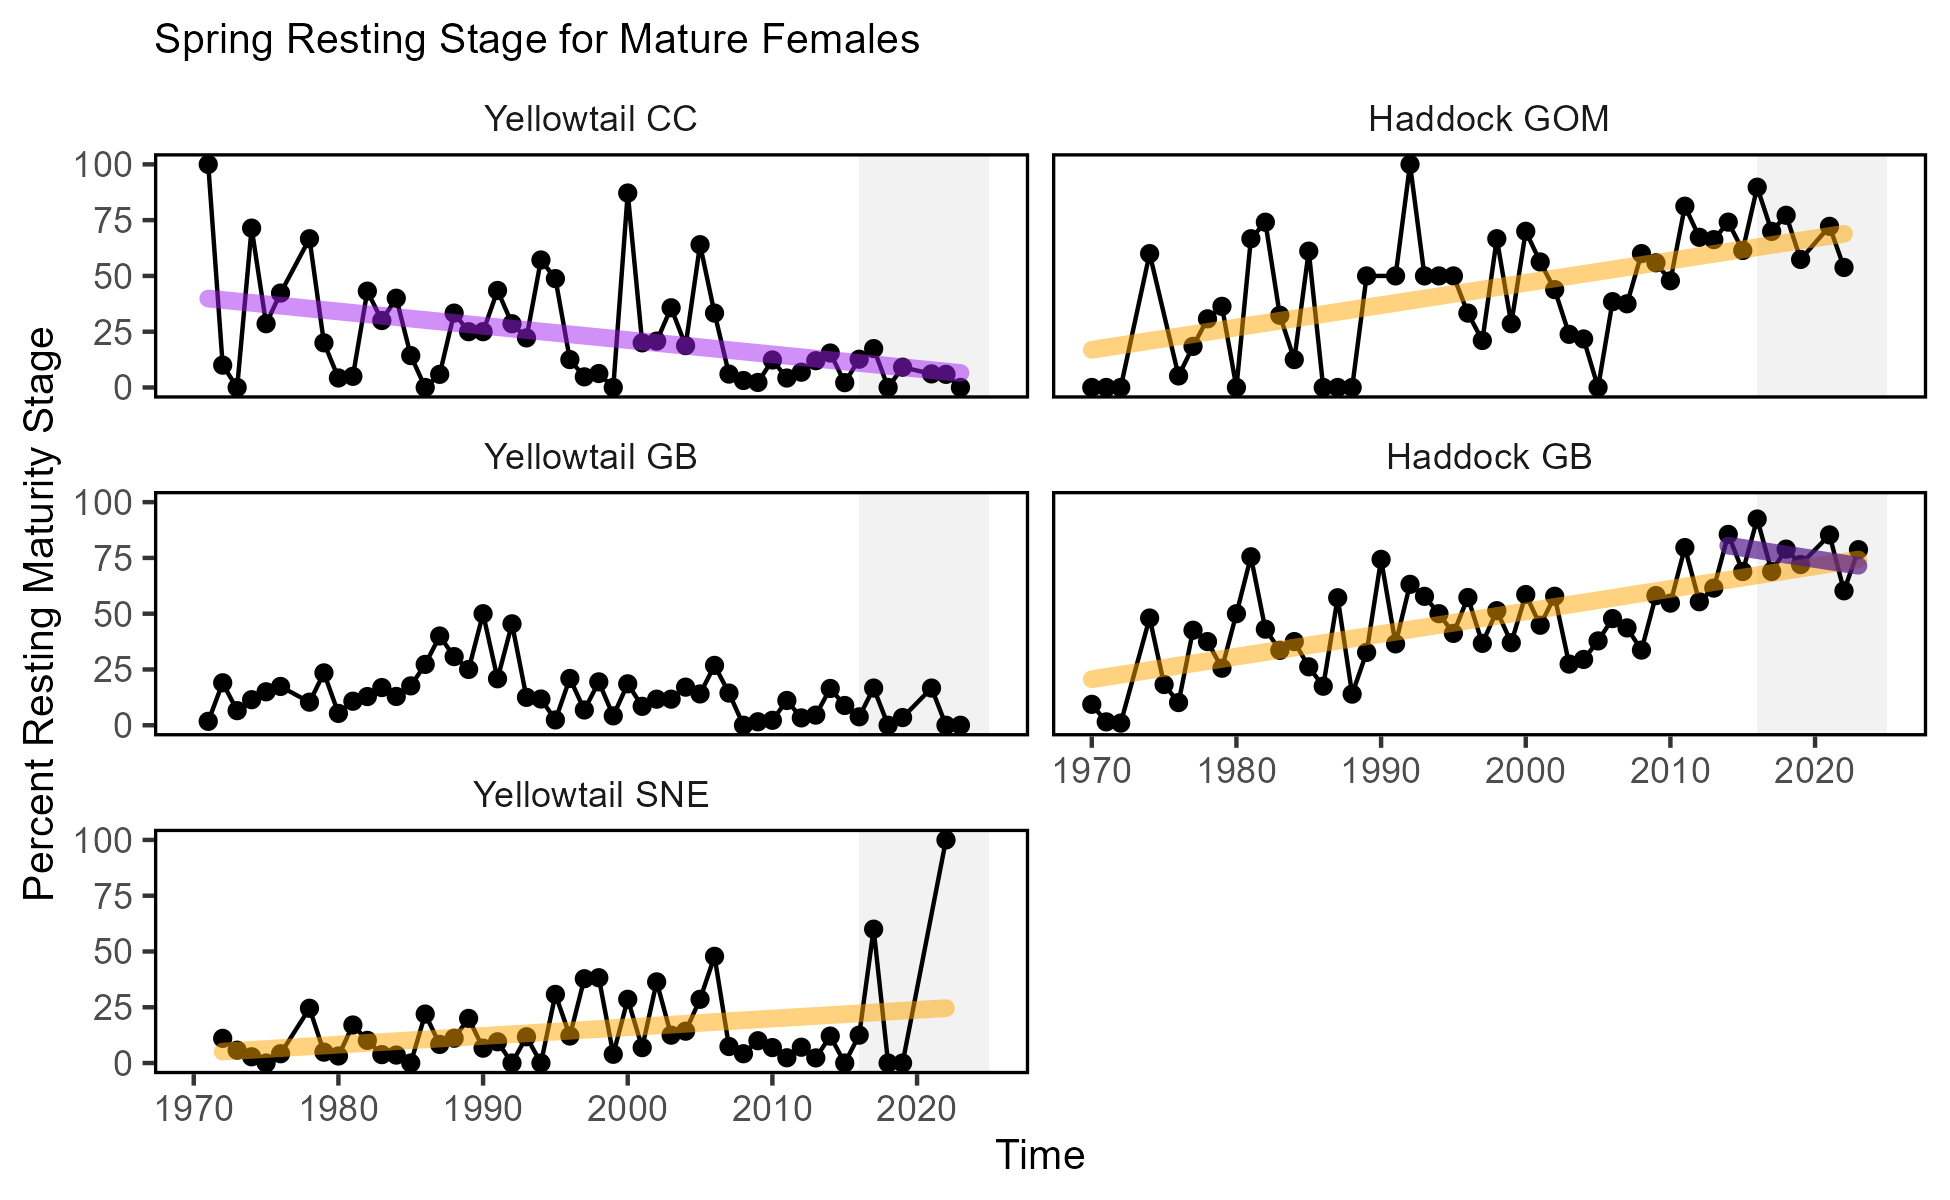
\includegraphics[width=1\linewidth,]{images/BothReports/spawn_timing_BothReports_2026-03-26} 

}

\caption{Percent resting stage (non-spawning) mature female fish (black) from spring Northeast Fisheries Science Center bottom trawl survey with significant long-term increases (orange), short-term decreases (dark purple), and long-term decreases (purple) from two haddock and three yellowtail flounder stocks: CC = Cape Cod, Gulf of Maine, GOM = Gulf of Maine, GB = Georges Bank, SNE = Southern New England.}\label{fig:spawntiming}
\end{figure}

\href{https://noaa-edab.github.io/catalog/timing_shifts.html}{Migration timing} of some tuna and large whales has changed. An analysis of recreational fishing data between 2019 and 2022 identified multiple shifts in important HMS species. For example, bigeye tuna were caught 50 days earlier; small and large bluefin tuna were caught 38 and 80 days earlier respectively in Massachusetts; and blue marlin in New York were caught 27 days earlier. A separate analysis of acoustic telemetry data predicted delayed departure of southward-migrating sharks from the northeast region under future sea surface temperatures. These results are further supported by the Atlantic Highly Migratory Species Climate Vulnerability Assessment, which found that 57 of 58 highly migratory species and stocks have high or very high potential to shift distributions. In Cape Cod Bay, \href{https://noaa-edab.github.io/catalog/timing_shifts.html}{peak spring habitat use} by right and humpback whales has shifted 18-19 days later between 1998 and 2018.

Understanding whether seasonal patterns are changing for stocks requires regular observations throughout the year. For example, baseline work on \href{https://noaa-edab.github.io/catalog/cetacean_acoustic.html}{cetacean presence in Southern New England} shows different seasonal use patterns for whale and dolphin species. Despite the importance of understanding seasonal patterns, we have few indicators that directly assess timing shifts of species. We plan on incorporating more indicators of timing shifts and phenology in future reports.

\paragraph{Drivers:}\label{drivers-1}

The drivers of timing shifts in managed stocks are generally coupled to shifts in environmental or biological conditions, since these can result in changes in habitat quality or food availability within the year. Changes in the timing of fall phytoplankton blooms and seasonal shifts in zooplankton communities are indicators of changes in seasonal food availability to stocks.

Along with the overall warming trends in the Mid-Atlantic Bight, ocean summer conditions have been lasting longer (Fig. \ref{fig:transition}) due to the earlier \href{https://noaa-edab.github.io/catalog/trans_dates.html}{transition} from cool spring conditions to warm summer conditions and the later transition from warm summer conditions to cooler fall temperatures. These transition dates relate how daily temperatures compare to the seasonal norm. Changes in the timing of seasonal environmental cycles can alter biological processes (migrations, spawning, etc.) that are triggered by seasonal events.

\begin{figure}[T]

{\centering 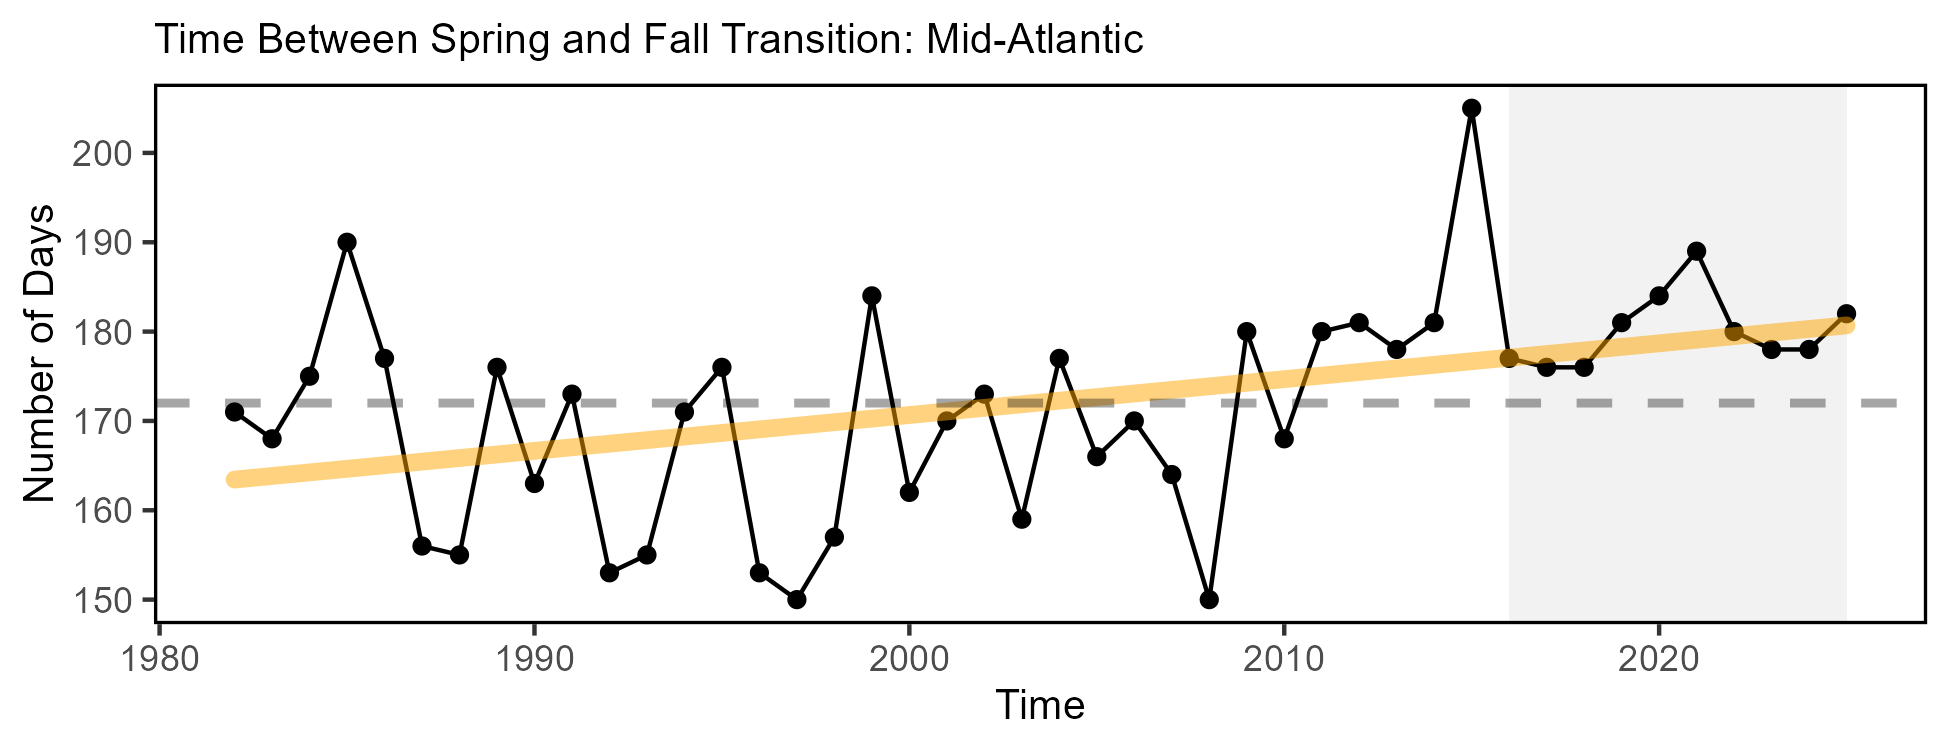
\includegraphics[width=1\linewidth,]{images/MidAtlantic/transition_date_MidAtlantic_2026-03-26} 

}

\caption{Ocean summer length in the Mid-Atlantic Bight: the annual total number of days between the spring thermal transition date and the fall thermal transition date (black), with a long-term increasing trend (orange). Transition dates are based on sea surface temperatures.}\label{fig:transition}
\end{figure}

\hyperref[climate-and-ecosystem-change]{As noted above}, the Mid-Atlantic \href{https://noaa-edab.github.io/catalog/cold_pool.html}{Cold Pool} is a summer to early fall feature that creates seasonally suitable habitat for some species. Cold Pool persistence has decreased; the average duration of the Cold Pool habitat is now shorter compared to the 1960s (Fig. \ref{fig:cold-pool-time}). However, all Cold Pool indices were near or above the long-term average in 2025 and likely related to the influx of northern waters into the system (see \href{https://noaa-edab.github.io/catalog/observation_synthesis_2024.html}{2024 Highlights} ). A change in the timing of the autumn breakdown of the Cold Pool may impact the recruitment of species that rely on it for seasonal cues and habitat. Southern New England-Mid-Atlantic yellowtail flounder recruitment and settlement are related to the strength of the MAB Cold Pool (a factor of extent and persistence). The correlation of pre-recruit settlers to the Cold Pool is thought to represent a bottleneck in yellowtail flounder life history, whereby a local and temporary increase in bottom temperature can negatively impact the survival of settlers. Including the effect of Cold Pool variations on yellowtail recruitment reduced retrospective patterns and improved predictive skill in a stock assessment model. This connection is especially important given the long-term decline in the duration of the Cold Pool.

\begin{figure}[T]

{\centering 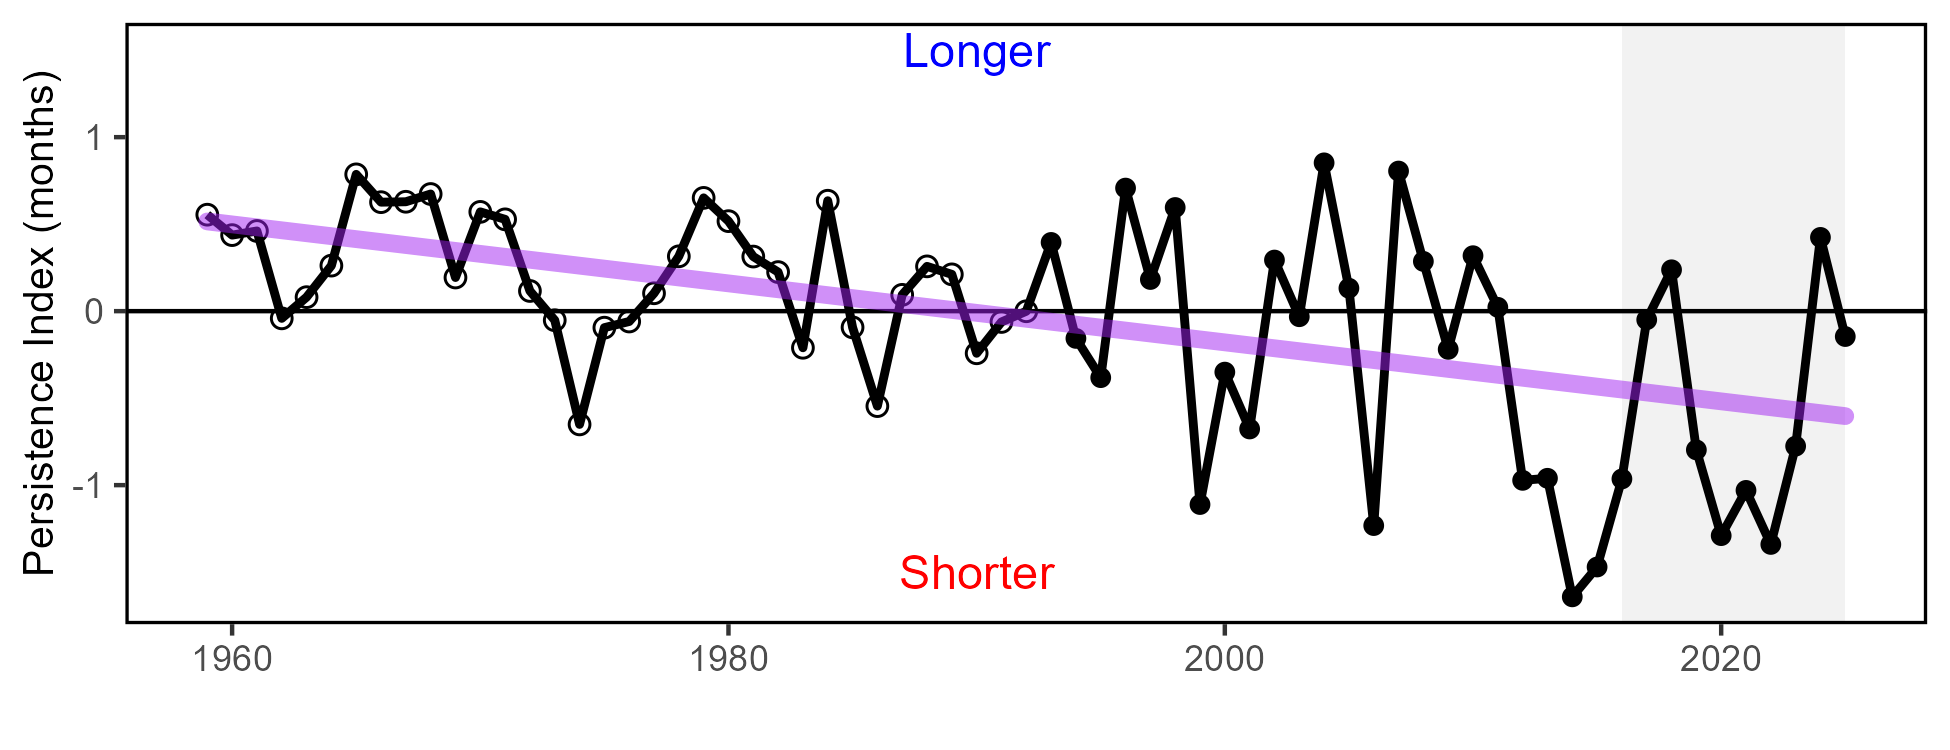
\includegraphics[width=1\linewidth,]{images/BothReports/cold_pool_time_BothReports_2026-03-26} 

}

\caption{The Mid-Atlantic Bight Cold Pool persistence index based on bias-corrected Regional Ocean Modeling System-Northwest Atlantic(open circles) and GLORYS (closed circles), with significant long-term decline (purple).}\label{fig:cold-pool-time}
\end{figure}

The seasonal timing of Mid-Atlantic \href{https://noaa-edab.github.io/catalog/chl_pp.html}{phytoplankton} blooms shows high interannual variability during the fall bloom period (October-December, Fig. \ref{fig:chl-month}). The significant increase in January chlorophyll suggests that the fall bloom period is continuing into the winter, with higher phytoplankton concentrations now than in the late 1990s. The significant decrease of chlorophyll in September could be related to warmer temperatures persisting into early fall and nutrient limitation causing a delay in the fall bloom. Changes to bloom timing can create a mismatch with the timing of larval fish development and may impact recruitment.

\begin{figure}[T]

{\centering 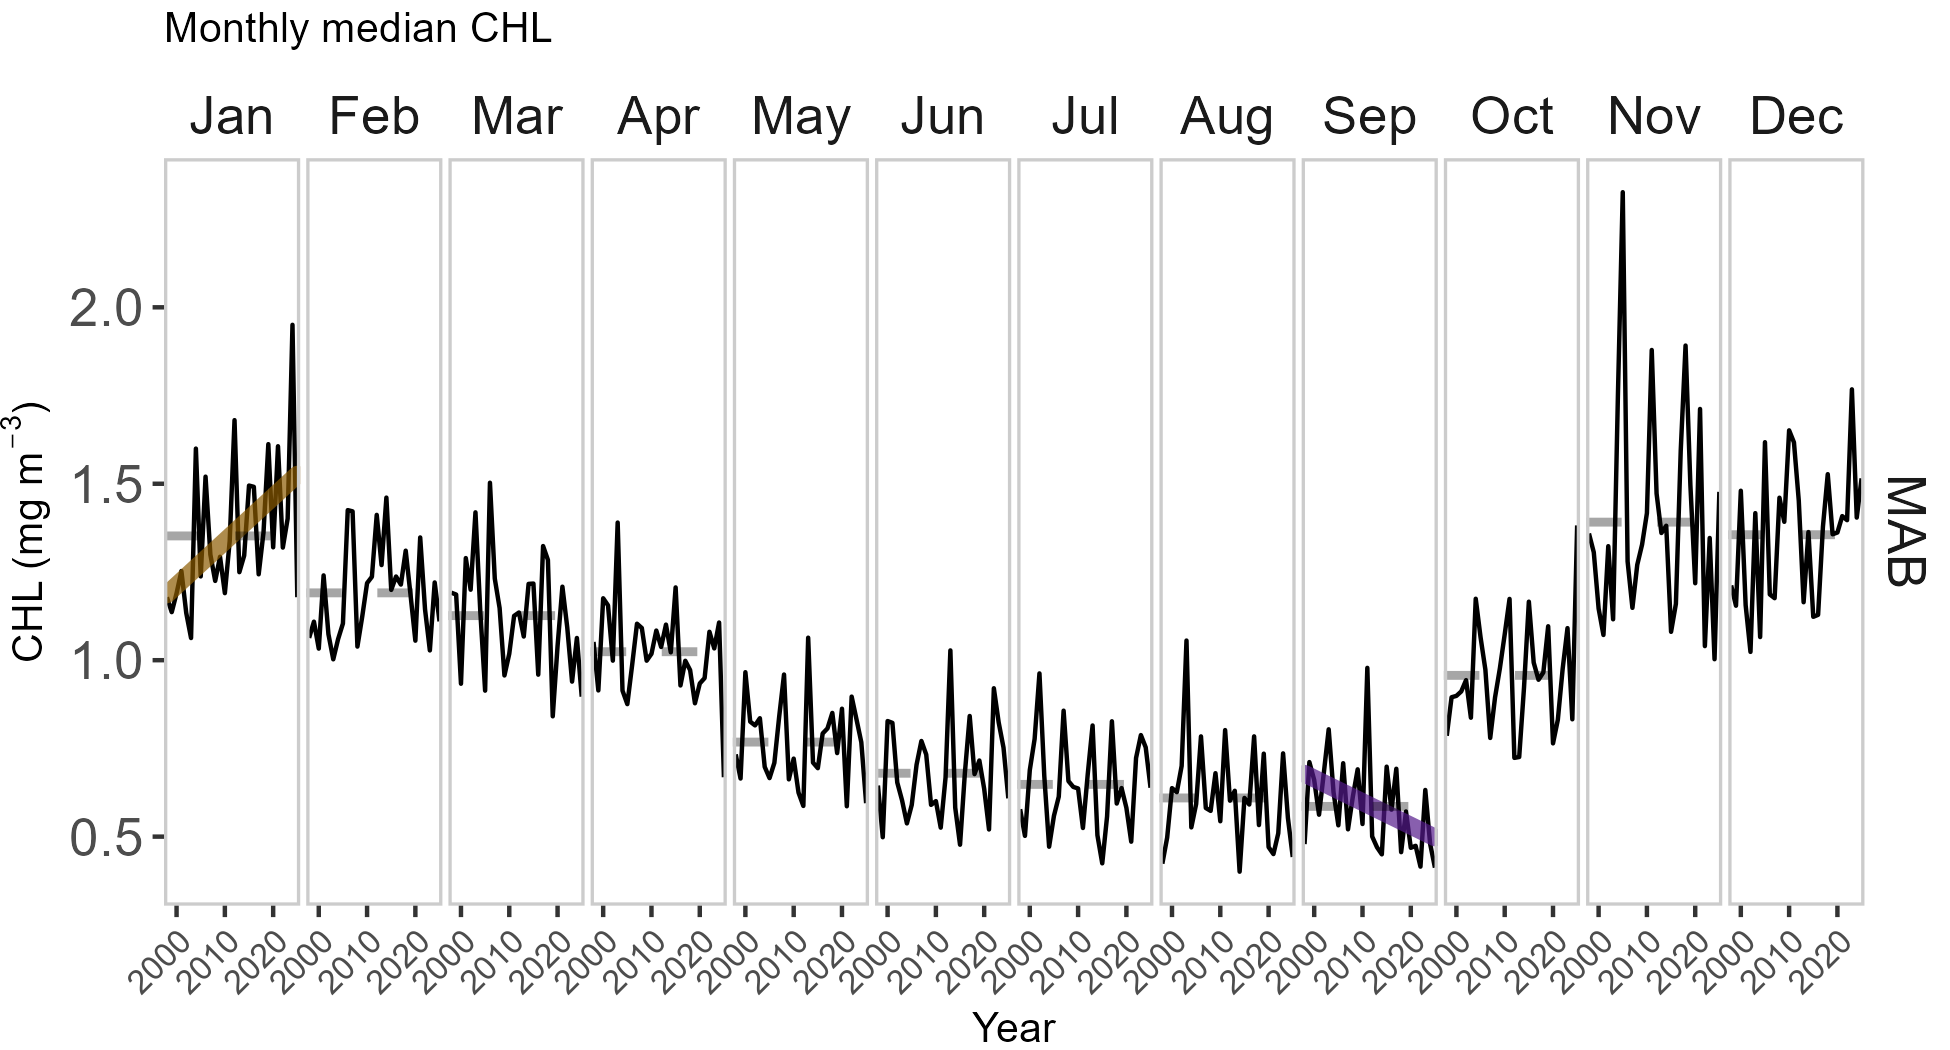
\includegraphics[width=1\linewidth,]{images/MidAtlantic/monthly_chl_MidAtlantic_2026-03-27} 

}

\caption{Monthly median chlorophyll a concentration in the Mid-Atlantic Bight (black) with a significant long-term increase present in January (orange) and a significant long-term decline in September (purple).}\label{fig:chl-month}
\end{figure}

\paragraph{Future Considerations}\label{future-considerations-1}

Species are reliant on environmental processes (e.g., phytoplankton bloom timing, thermal transition, or the duration of the Cold Pool) to dictate the timing of their behavior. Some changes are episodic and have interannual variability, while others may be shifting away from a historic baseline on the scales of years to decades. Other species may rely on the general seasonal succession of environmental drivers (e.g., the timing of the fall turnover) to cue biological processes, and long-term trends in seasonal transitions are unlikely to reverse in coming years. Thus, timing shifts in migration or spawning may continue. Management actions that rely on effective alignment of fisheries availability and biological processes should continue to evaluate whether prior assumptions on seasonal timings still hold, and new indicators should be developed to monitor timing shifts for stocks.

\subsubsection{Risks to setting catch limits}\label{risks-to-setting-catch-limits}

The efficacy of short-term stock projections and rebuilding plans rely on accurate understanding of processes affecting stock growth, reproduction, and natural mortality. These biological processes are often driven by underlying environmental change. If not considered in management, environmental change may increase the risk that established stock-level biological reference points no longer reflect the current population and increase projection uncertainty, both of which can contribute to quota misspecification.

\paragraph{Indicators: Fish productivity and condition shifts}\label{indicators-fish-productivity-and-condition-shifts}

Indicators of \href{https://noaa-edab.github.io/catalog/productivity_anomaly.html}{fish productivity} are derived from observations (surveys) or models (stock assessments). Fish productivity declined during the 1990s and 2000s with declining production of summer flounder and has been variable since, as described by the small-fish-per-large-fish anomaly indicator (derived from NEFSC bottom trawl survey) (Fig. \ref{fig:productivity-anomaly}). Bluefish, black sea bass, and goosefish have sporadic years with large positive anomalies, but most years have small negative anomalies. This decline in fish productivity is also shown by a similar analysis based on stock assessment model outputs (recruitment per spawning stock biomass anomaly). Most species had positive recruitment anomalies in the 1990s and 2000s and are currently showing negative anomalies, indicating a decline in productivity. Fish productivity can be affected by parental condition, environmental conditions, timing and availability of prey for recruits, as well as retention of recruits within favorable habitat. High offshore advection during spawning seasons can reduce recruitment success and affect overall fish productivity.

The health of individual fish (i.e., fish condition, measured as weight for a given length) can contribute to population productivity through improved growth, reproduction and survival. Mid-Atlantic \href{https://noaa-edab.github.io/catalog/condition.html}{fish condition} was generally high to very high prior to 2000, low to very low from 2001-2010 (concurrent with declines in productivity, Fig. \ref{fig:productivity-anomaly}), and mixed since 2011. In 2025, condition continued to be mixed, with general improvement since a relatively low condition year in 2021 (Fig. \ref{fig:mab-cf}). Preliminary analyses show that years dominated by small copepods and warmer spring temperatures may improve fish condition for Atlantic mackerel and butterfish. Similar environmental drivers may be important to other species.

\begin{figure}[T]

{\centering 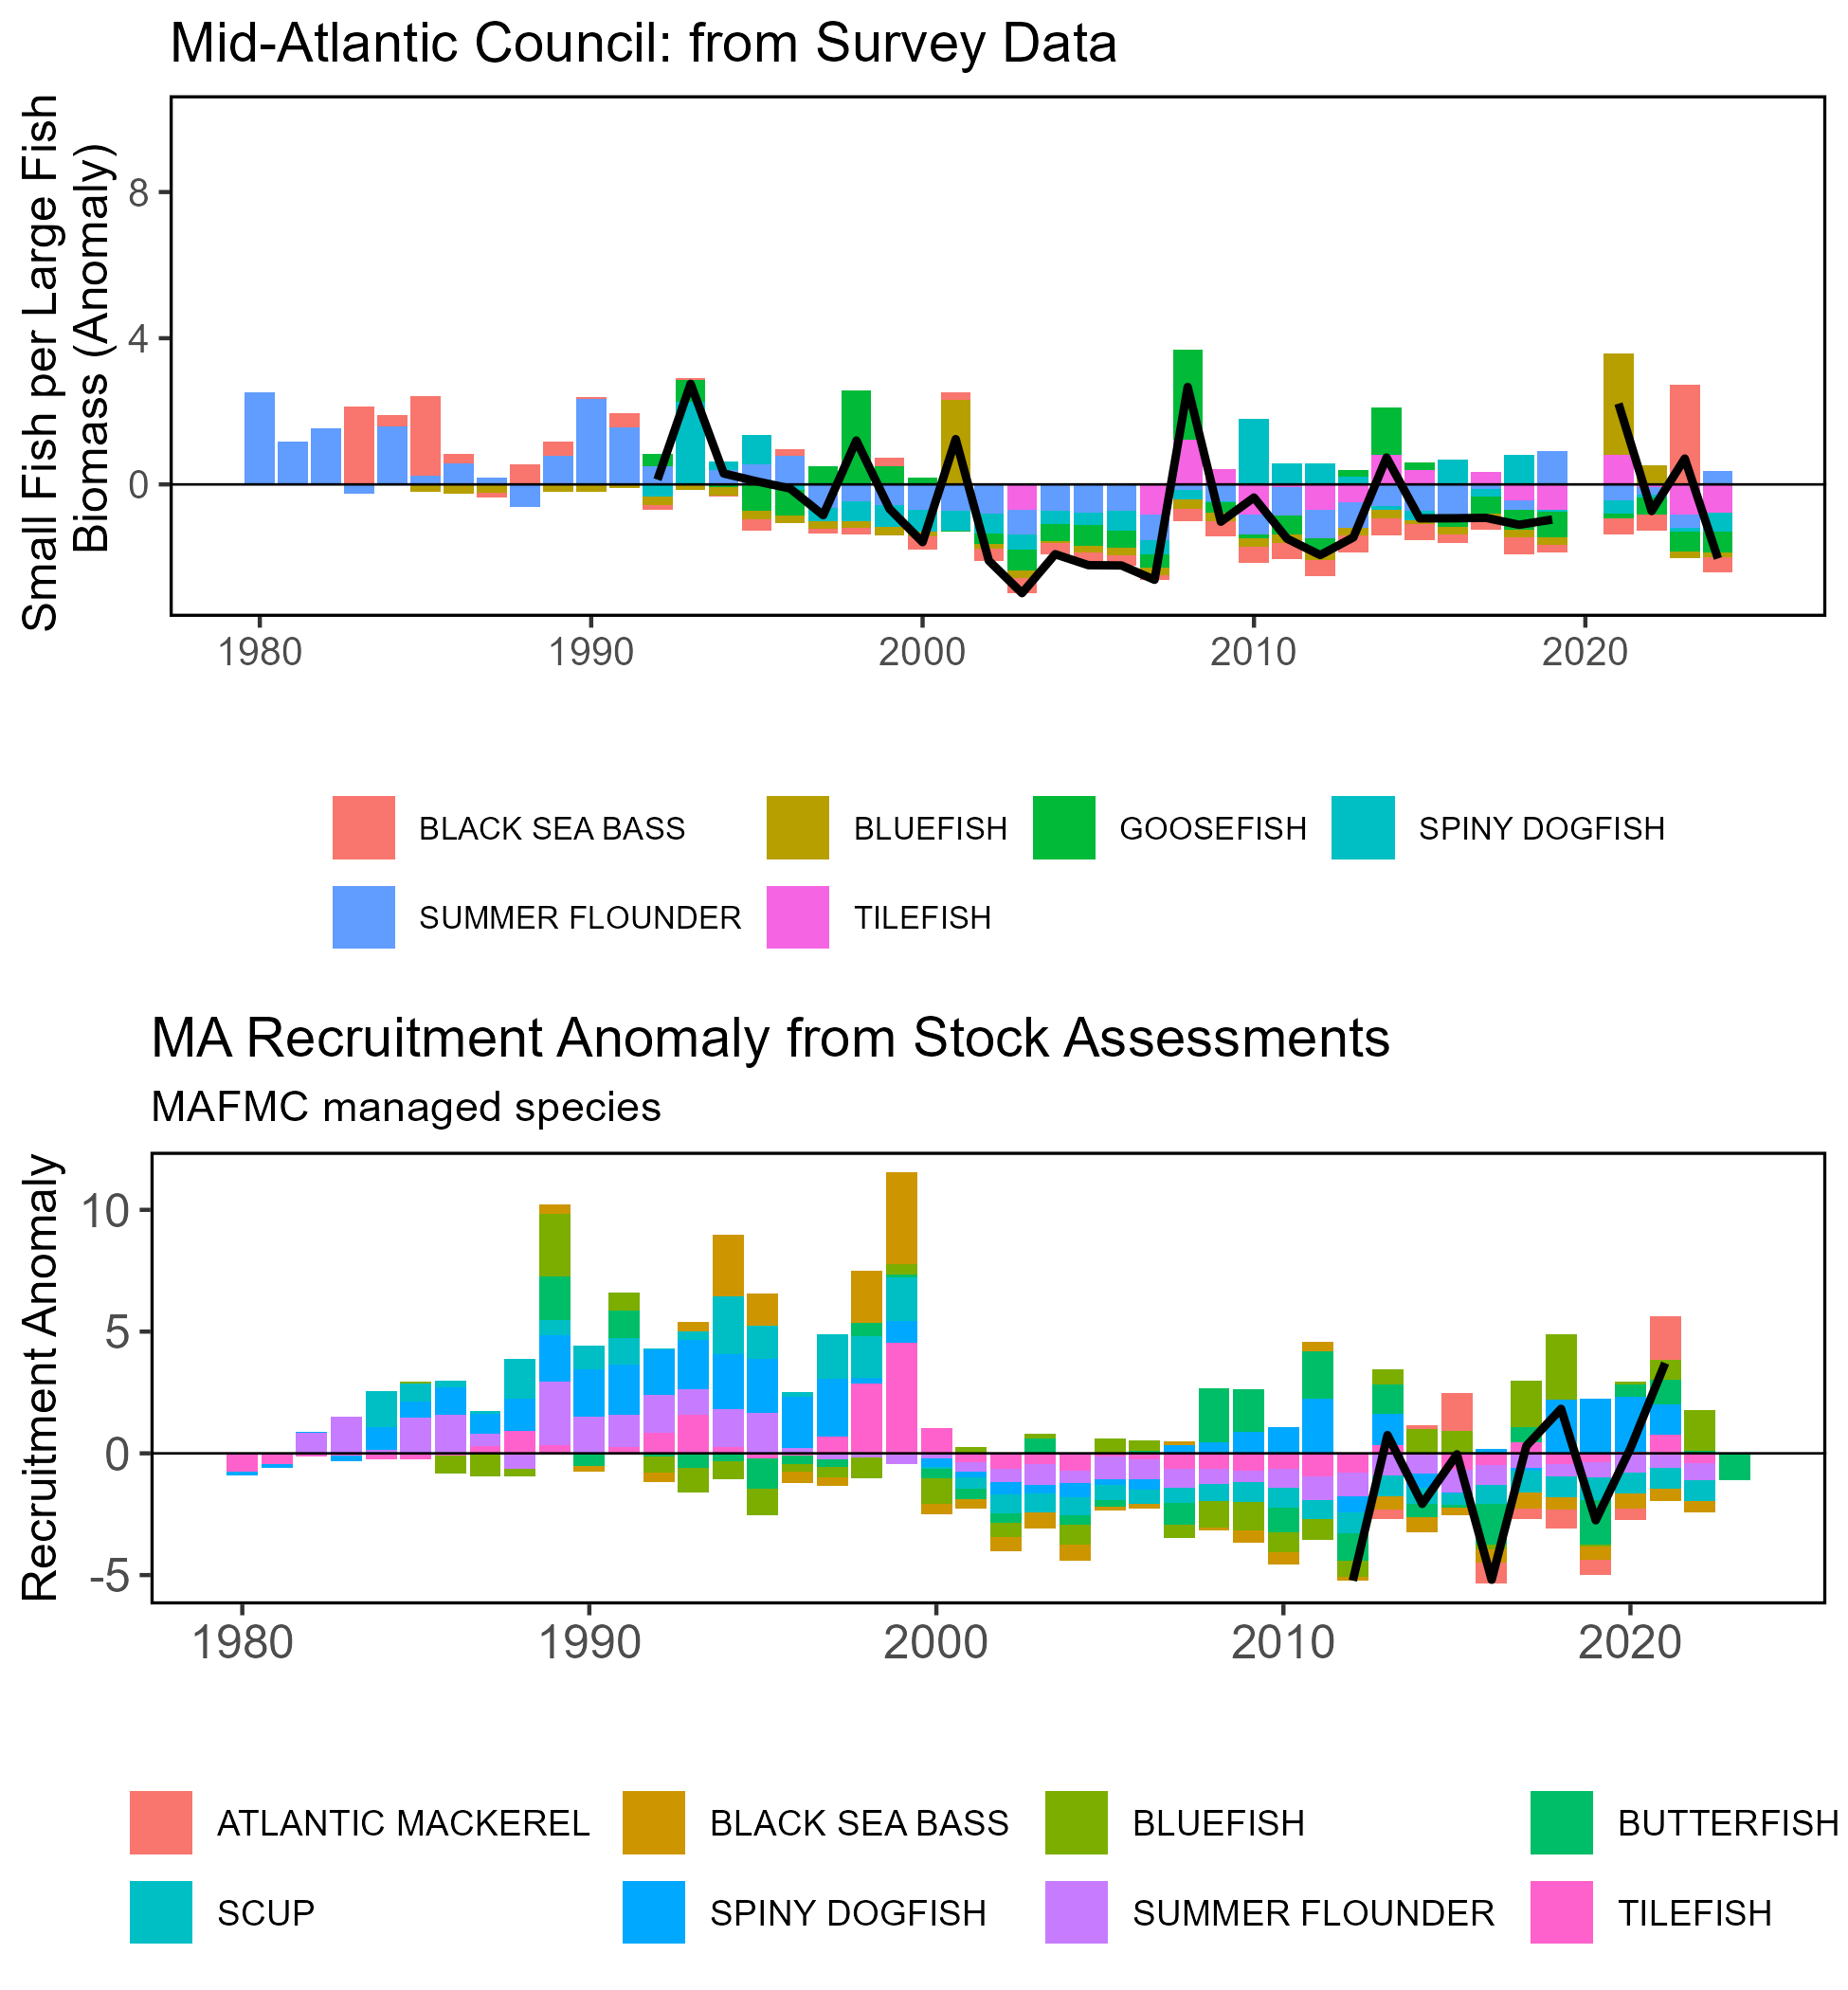
\includegraphics[width=1\linewidth,]{images/MidAtlantic/productivity_anomaly_MidAtlantic_2026-03-26} 

}

\caption{Fish productivity measures. Top: Small fish per large fish survey biomass anomaly of Mid-Atlantic Fishery Management Council (MAFMC) managed species in the Mid-Atlantic Bight. Bottom: assessment recruitment per spawning stock biomass anomaly for stocks managed by the MAFMC. The summed anomaly across species is shown by the black line, drawn across all years with the same number of stocks analyzed.}\label{fig:productivity-anomaly}
\end{figure}

\begin{figure}[T]

{\centering 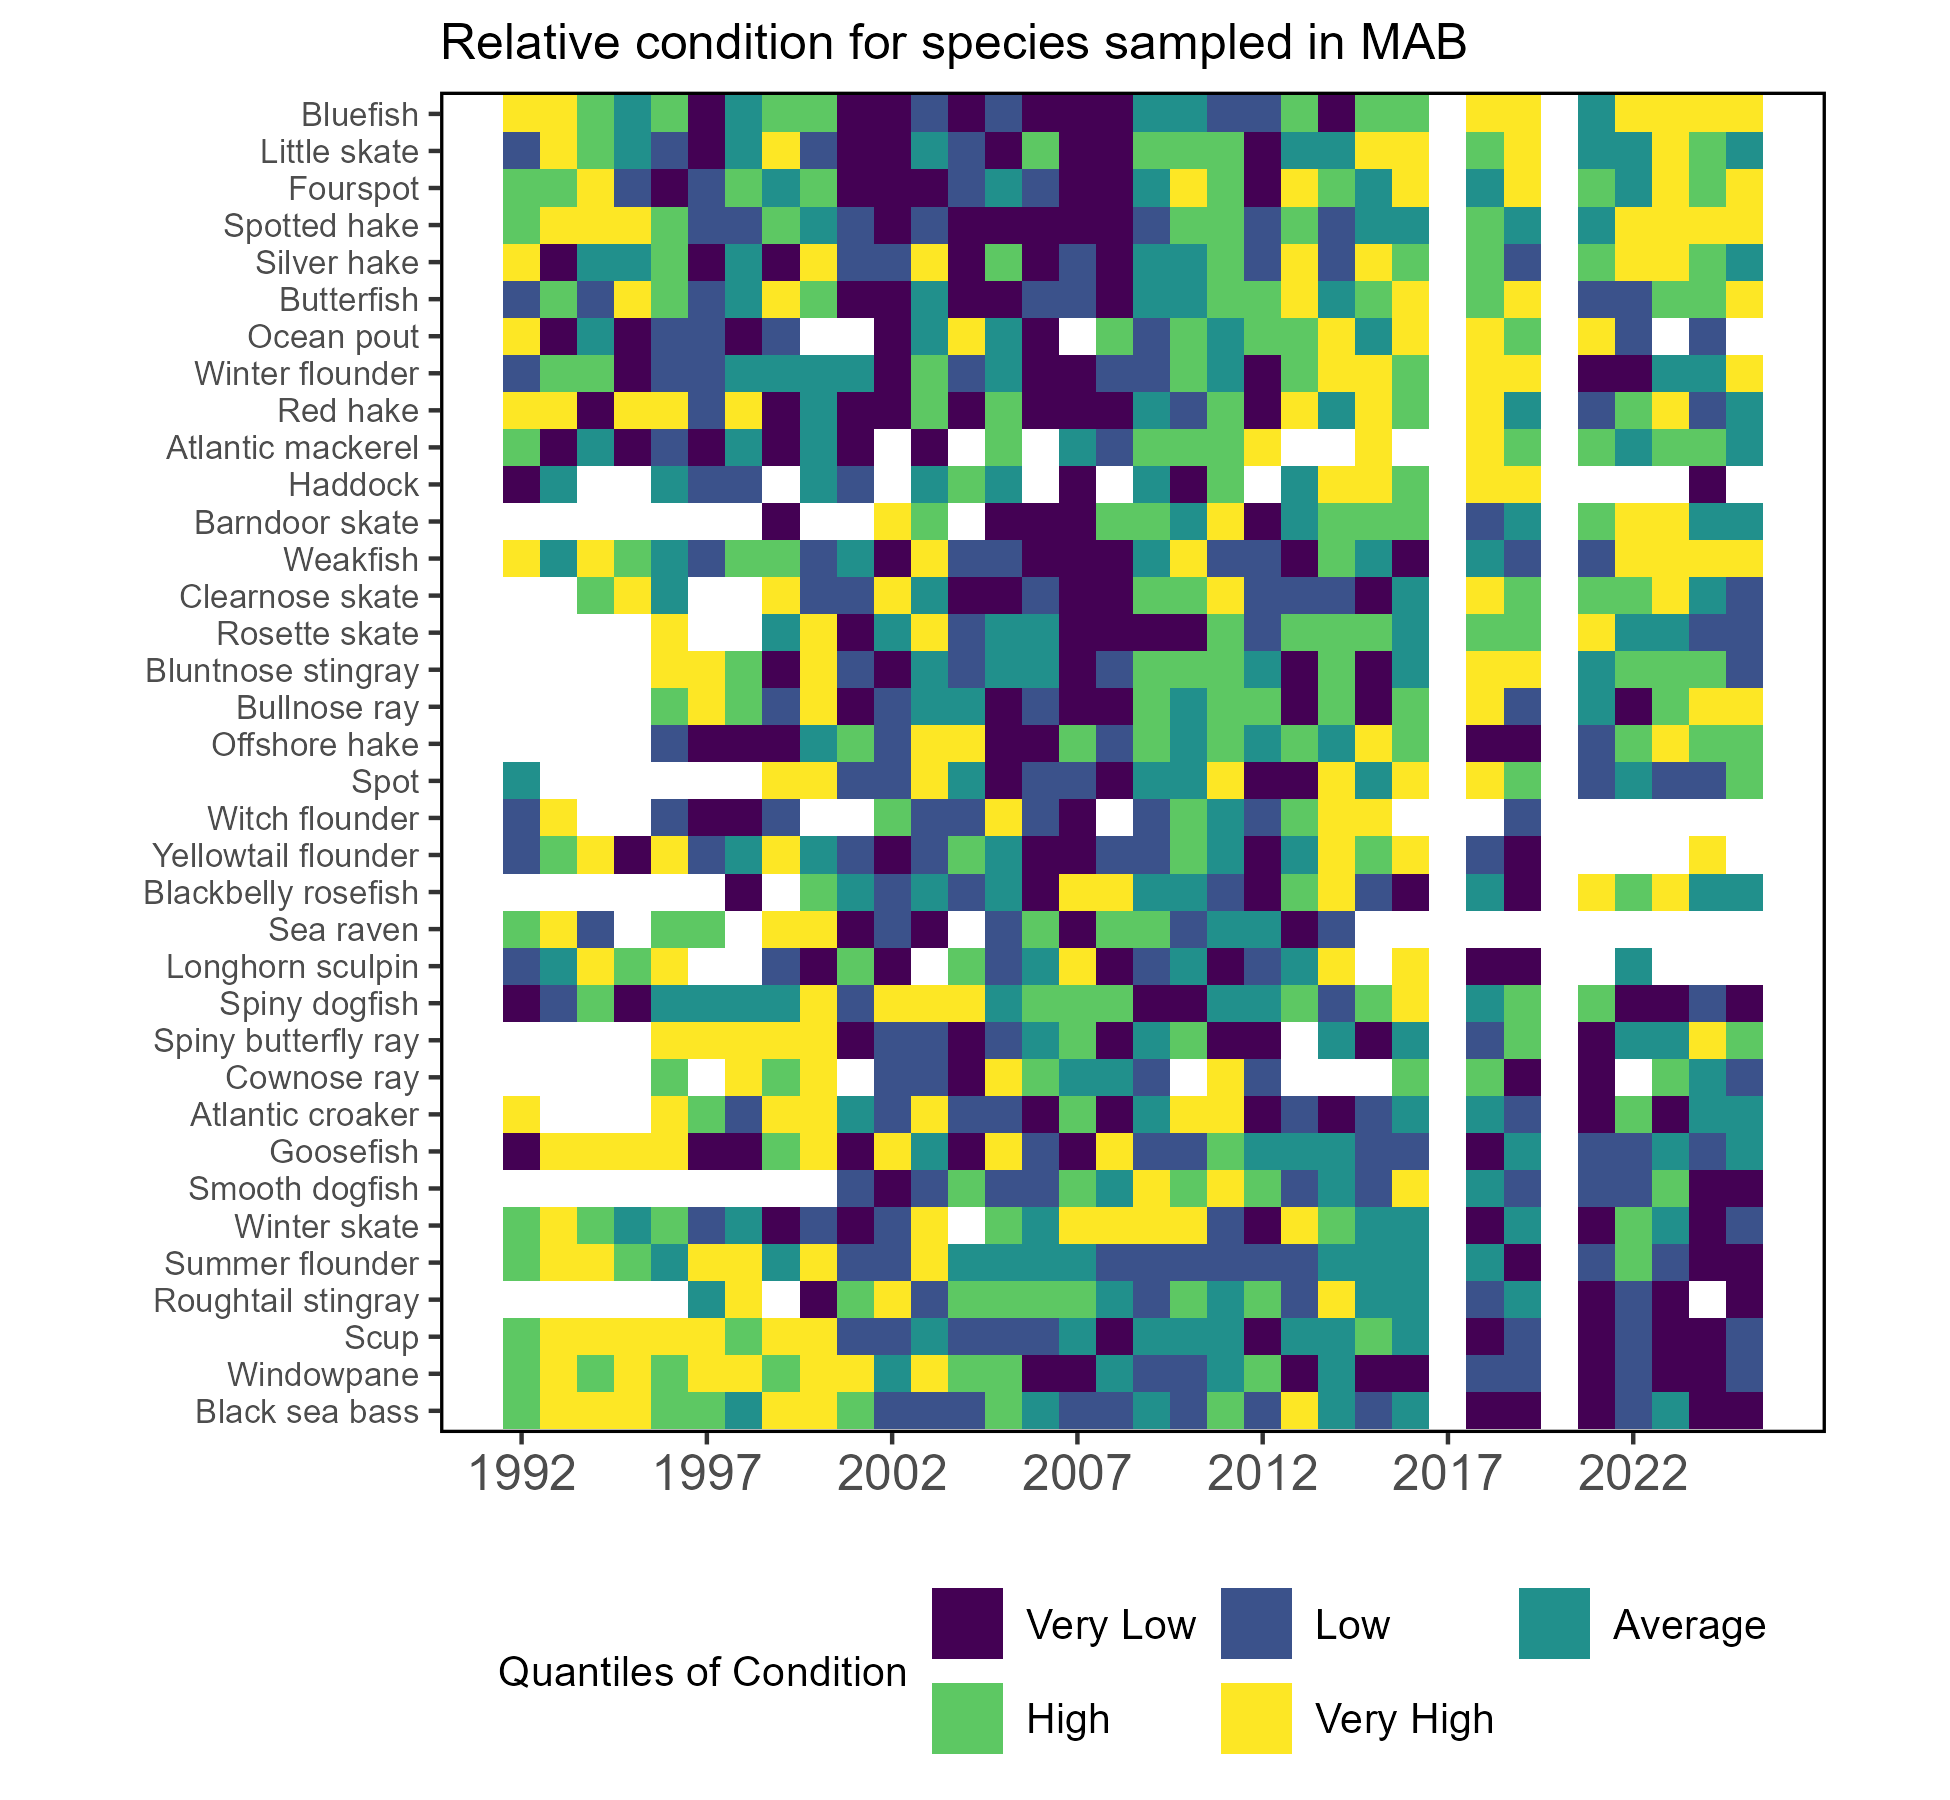
\includegraphics[width=1\linewidth,]{images/MidAtlantic/condition_MidAtlantic_2026-03-26} 

}

\caption{Condition factor for fish species in the Mid-Atlantic Bight (MAB) based on fall Northeast Fisheries Science Center bottom trawl survey data. MAB data are missing for 2017 due to survey delays, and no survey was conducted in 2020.}\label{fig:mab-cf}
\end{figure}

\paragraph{Drivers:}\label{drivers-2}

Fish productivity and condition are the cumulative effects of physiological, ecological, and environmental factors. Major factors include increased metabolic demands from increasing temperature and changes in the availability and quality of prey. Long-term environmental trends and episodic extreme temperatures, ocean acidification, and low oxygen events represent multiple stressors that can affect growth rates, reproductive success, recruitment, and cause mortality.

\subparagraph{Biological Drivers: Forage quality and abundance}\label{biological-drivers-forage-quality-and-abundance}

The energy density (ED) of prey, in conjunction with its mass, indicates the total amount of energy available to higher trophic level predators. The quality and abundance of this forage base directly impact the productivity and movement of managed and protected species. Management should consider these energetic links, as shifts in forage quality can alter the health of individual stocks and the entire ecosystem.

Forage fish \href{https://noaa-edab.github.io/catalog/energy_density.html}{energy content} fluctuates based on growth, reproduction, environmental conditions, and ecosystem productivity. In the Mid-Atlantic Bight, butterfish are the most abundant high ED forage species (Fig. \ref{fig:energy-density}), though their fall ED has recently declined toward lower spring averages. Atlantic herring and Atlantic mackerel also serve as high-energy prey, but herring show recently low ED and declining abundance, while mackerel are most abundant in the spring despite having higher ED in the fall. Moderate energy forage species (longfin squid, northern shortfin squid, and silver hake) are of intermediate abundance and show minimal annual and seasonal variation in ED. Other species have high ED but lower abundance decreasing their reliability as a food source.

\begin{figure}[T]

{\centering 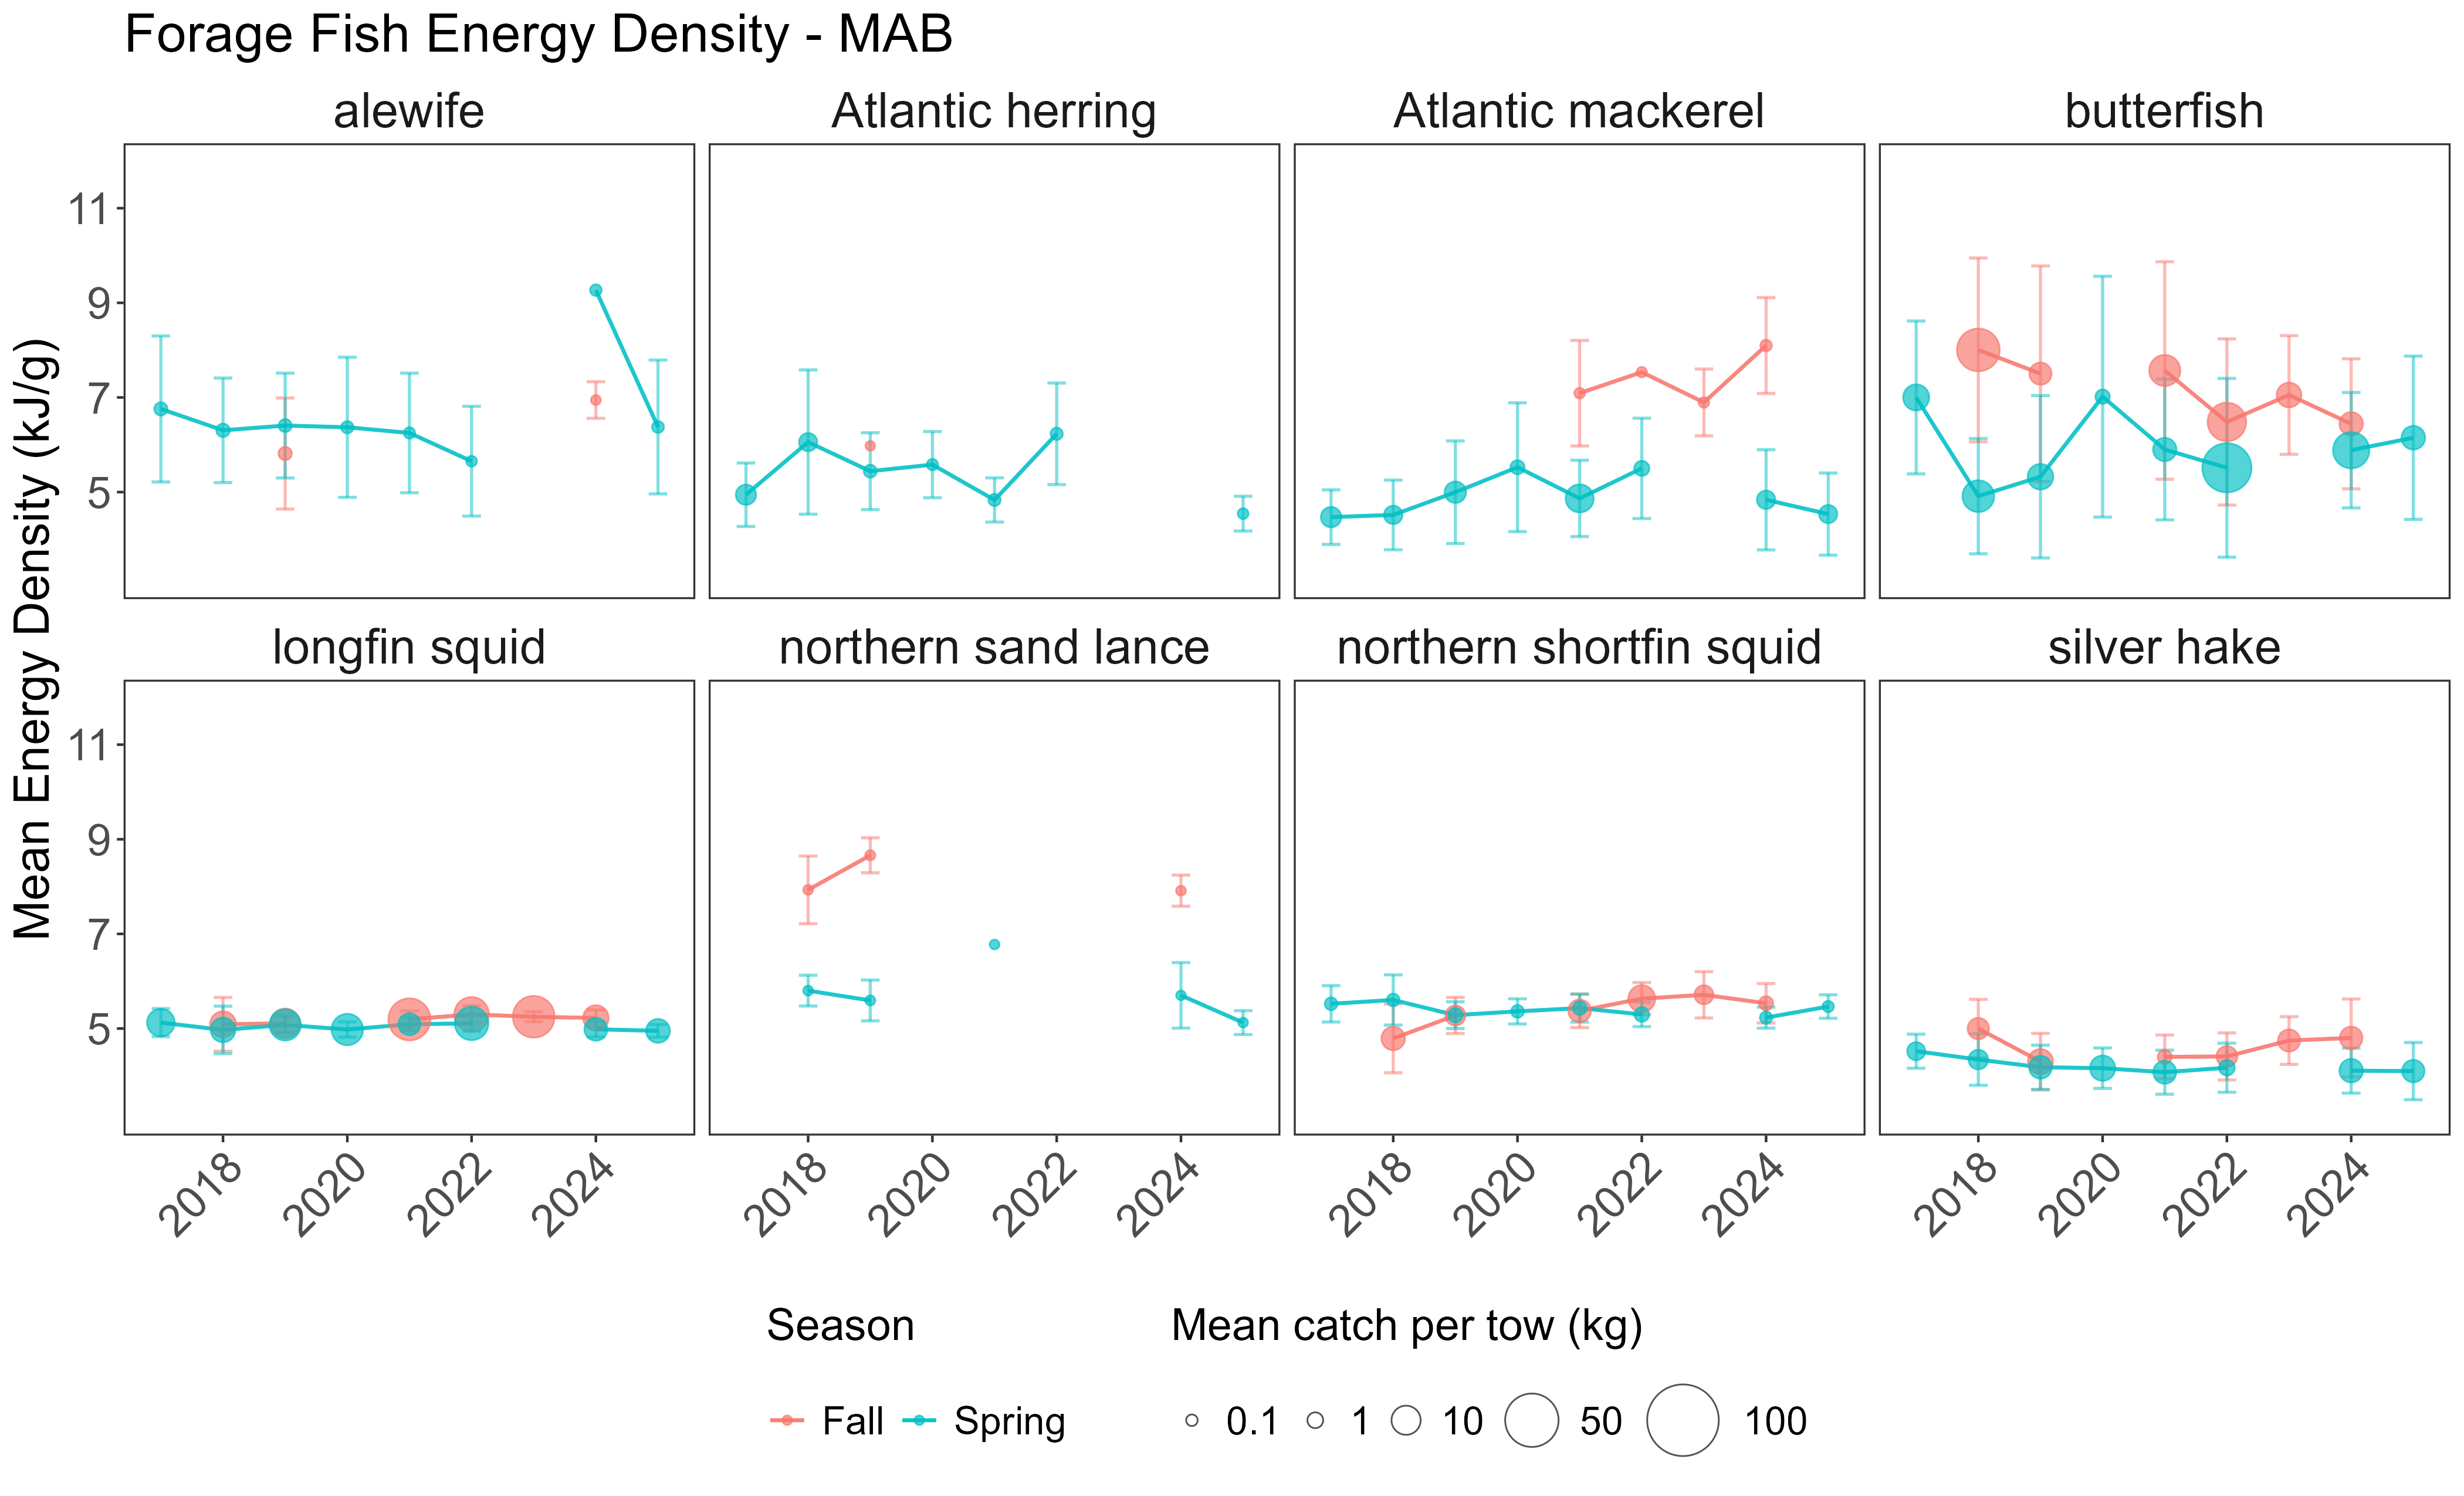
\includegraphics[width=1\linewidth,]{images/MidAtlantic/energy_density_MidAtlantic} 

}

\caption{Energy density (mean and standard deviation) of eight forage species from Northeast Fisheries Science Center bottom trawl surveys by season and year for the Mid-Atlantic Bight (MAB). Symbol size represents abundance (mean kg/tow) estimated from bottom trawl survey tows in the MAB.}\label{fig:energy-density}
\end{figure}

Changes in the overall abundance of forage fish can influence managed species productivity as it relates to changes in food availability. A spatially-explicit \href{https://noaa-edab.github.io/catalog/forage_index.html}{forage index} for the Mid-Atlantic shows a long term declining trend in fall, with higher forage biomass in fall than spring (Fig. \ref{fig:foragebio}). Forage biomass was highest during fall in the early-1980s. The decrease of fall forage biomass in the Mid-Atlantic may reduce the health and reproductive output of fish species. Additionally, this may be exacerbated by lower energy densities of prey, especially in years of higher water temperatures when metabolic demands are higher.

\begin{figure}[T]

{\centering 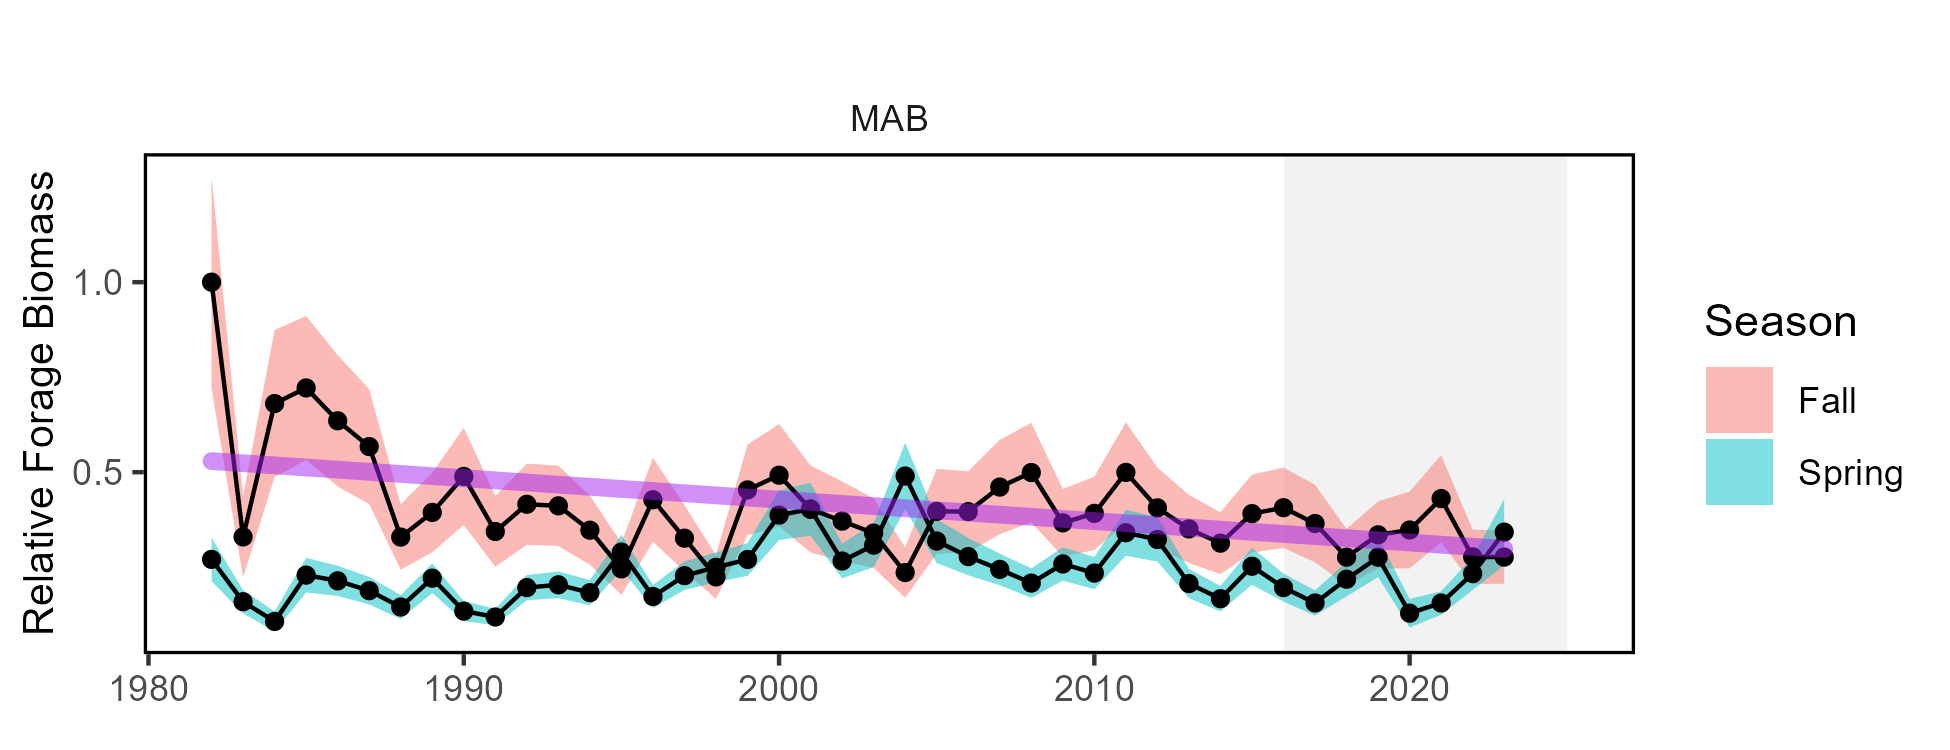
\includegraphics[width=1\linewidth,]{images/MidAtlantic/foragebio_MidAtlantic_2026-03-26} 

}

\caption{Forage fish index in the Mid-Atlantic Bight for spring (blue) and fall (red) surveys, with a long-term decline (purple) in fall. Index values are relative to the maximum observation within a region across surveys.}\label{fig:foragebio}
\end{figure}

\href{https://noaa-edab.github.io/catalog/benthos_index.html}{Benthic invertebrates} are extremely important forage for some managed species (e.g., black sea bass). Macrobenthos are small benthic organisms that tend to be prey for larger benthos and benthivores. Macrobenthos indices show long-term declines in spring (Fig. \ref{fig:benthos}), indicating a potential decrease in food availability for their predators. In contrast, Mid-Atlantic megabenthos indices show long-term increases in spring. Fish productivity may be negatively impacted in recent years for juvenile fish that target macrobenthos, such as small crustaceans and polychaetes, and positively impacted for fish such as black sea bass and striped bass that target megabenthos such as crabs. Other species that are generalist feeders such scup and skates may not be as impacted by offsetting trends in the benthic community.

\begin{figure}[T]

{\centering 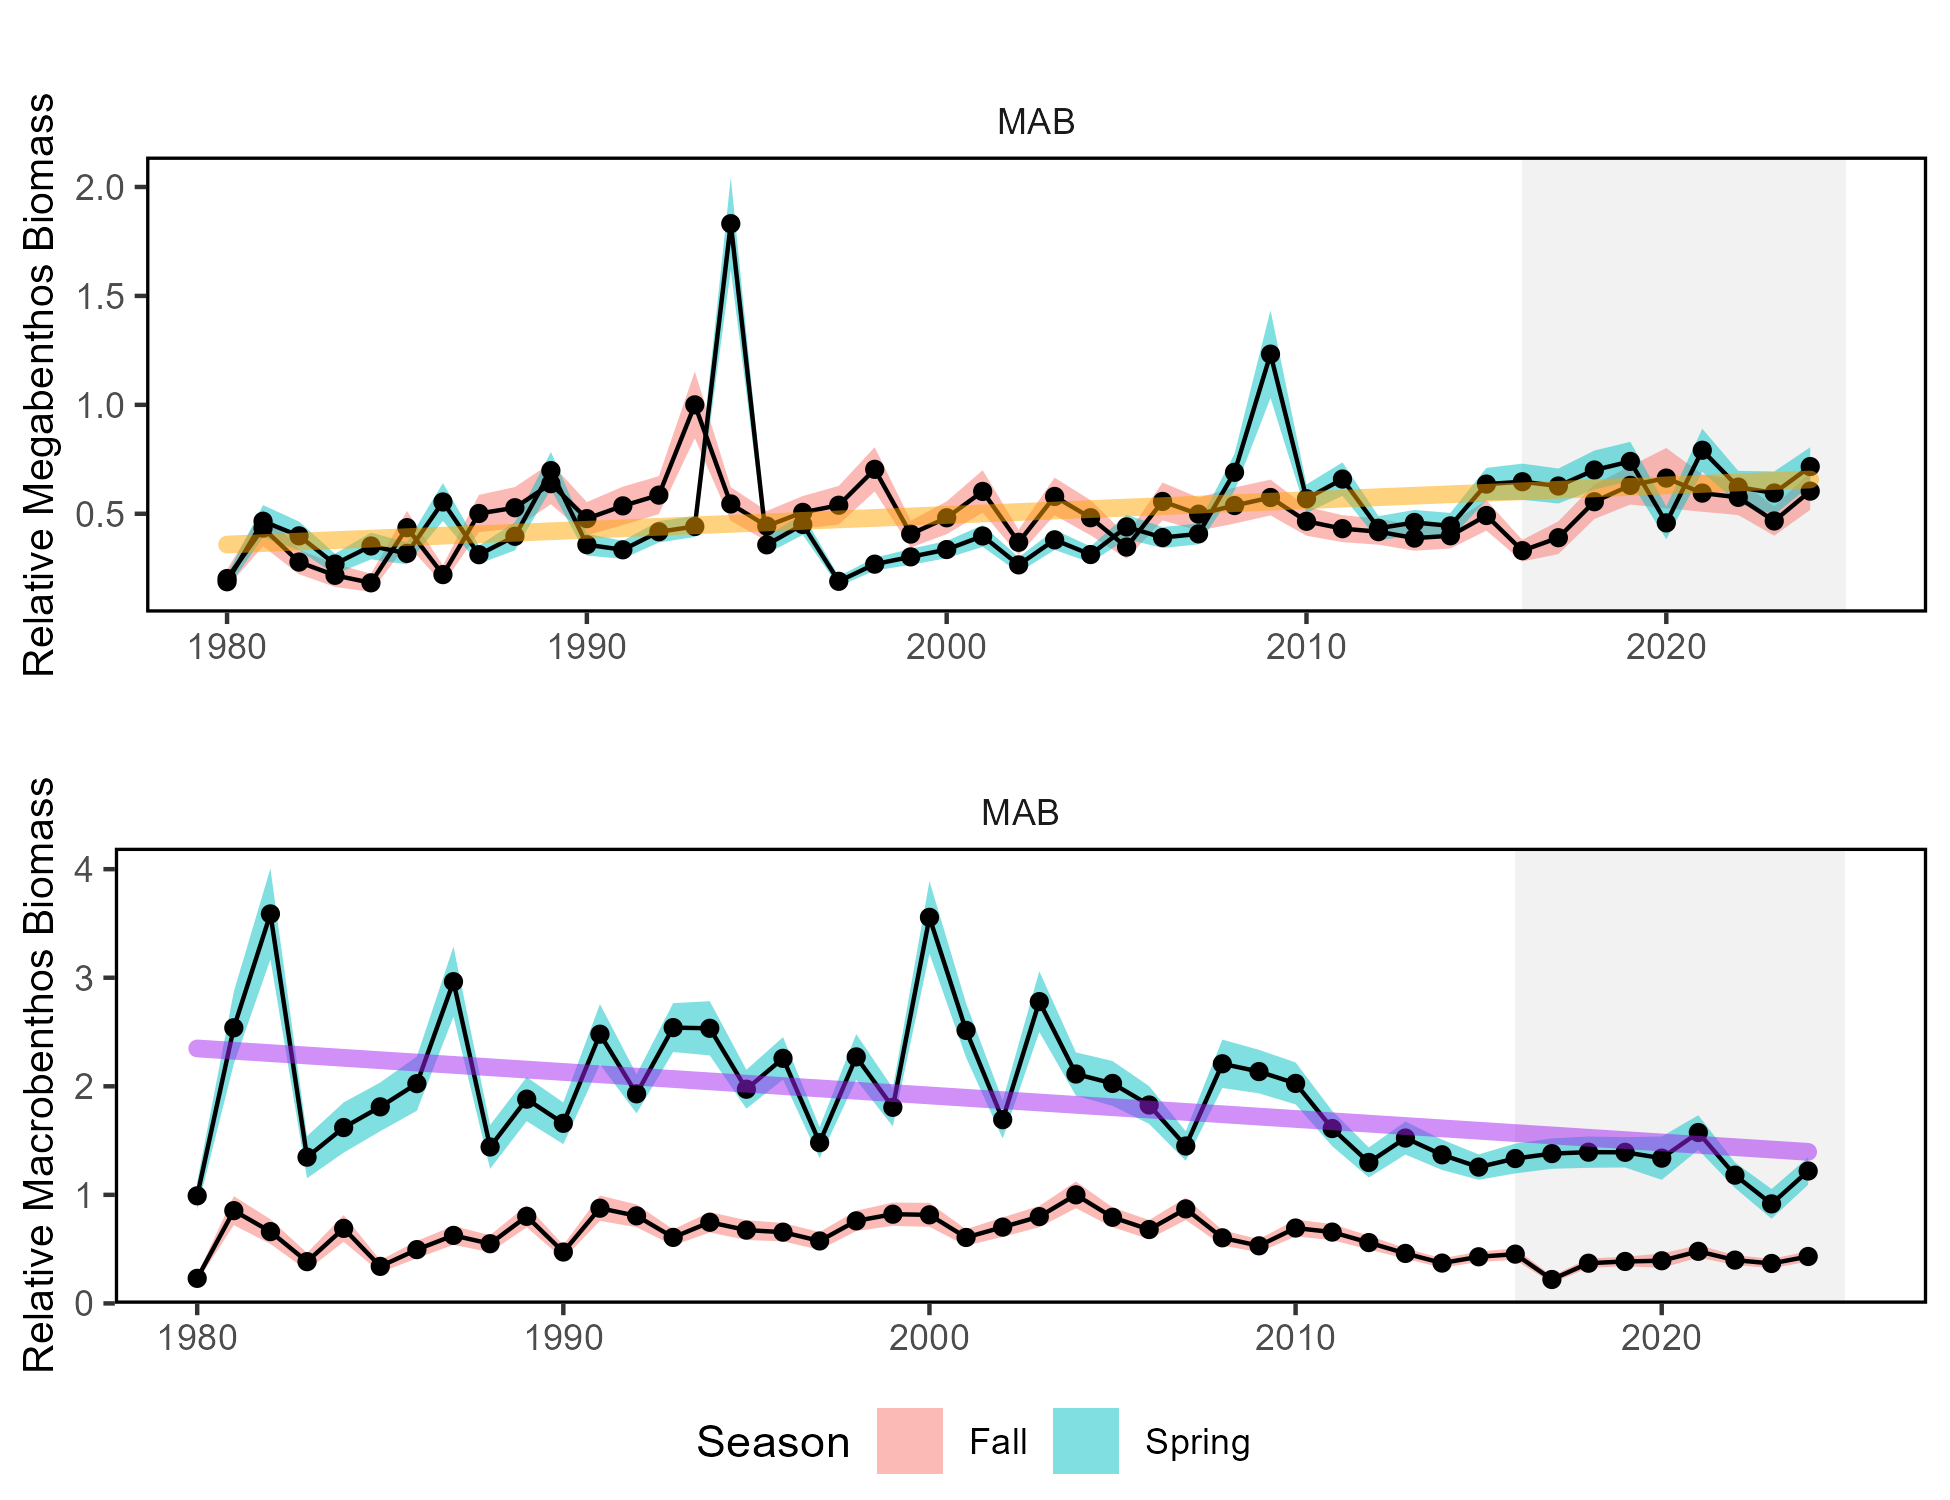
\includegraphics[width=1\linewidth,]{images/MidAtlantic/benthos_MidAtlantic_2026-03-27} 

}

\caption{Changes in spring (blue) and fall (red) benthos abundance in the Mid-Atlantic Bight for megabenthos (top) and macrobenthos (bottom), with significant long-term increasing trend (orange) for megabenthos and long-term decreasing trend (purple) for macrobenthos in spring.}\label{fig:benthos}
\end{figure}

\subparagraph{Biological Drivers: Lower trophic levels}\label{biological-drivers-lower-trophic-levels}

\href{https://noaa-edab.github.io/catalog/chl_pp.html}{Phytoplankton} are the foundation of the food web and are the primary food source for zooplankton and filter feeders such as shellfish. Multiple environmental and oceanographic drivers affect the abundance, \href{https://noaa-edab.github.io/catalog/chl_pp.html}{composition}, spatial distribution, and productivity of phytoplankton. While changes in phytoplankton productivity could affect fish productivity (including the productivity of forage fish), there is no clear long-term trend in Mid-Atlantic total primary production (Fig. \ref{fig:totpp}).

Changing \href{https://noaa-edab.github.io/catalog/zoo_abundance_anom.html}{zooplankton abundance} abundance may impact forage fish energy content and abundance, as well as the prey field of filter feeding whales, and managed species through food web impacts. Mid-Atlantic indices show high variability without a clear trend for large copepods, while small-bodied copepods show long-term and recent decreases, and krill (Euphausiids) show increasing trends (Fig. \ref{fig:zoopanom}). Energy density varies by season and location, with high-energy large copepods most abundant on the Northeast shelf from \href{https://noaa-edab.github.io/catalog/preyfield_energy.html}{April through June}. The community is undergoing a systemic shift away from copepod dominance and toward increased krill presence.

\begin{figure}[T]

{\centering 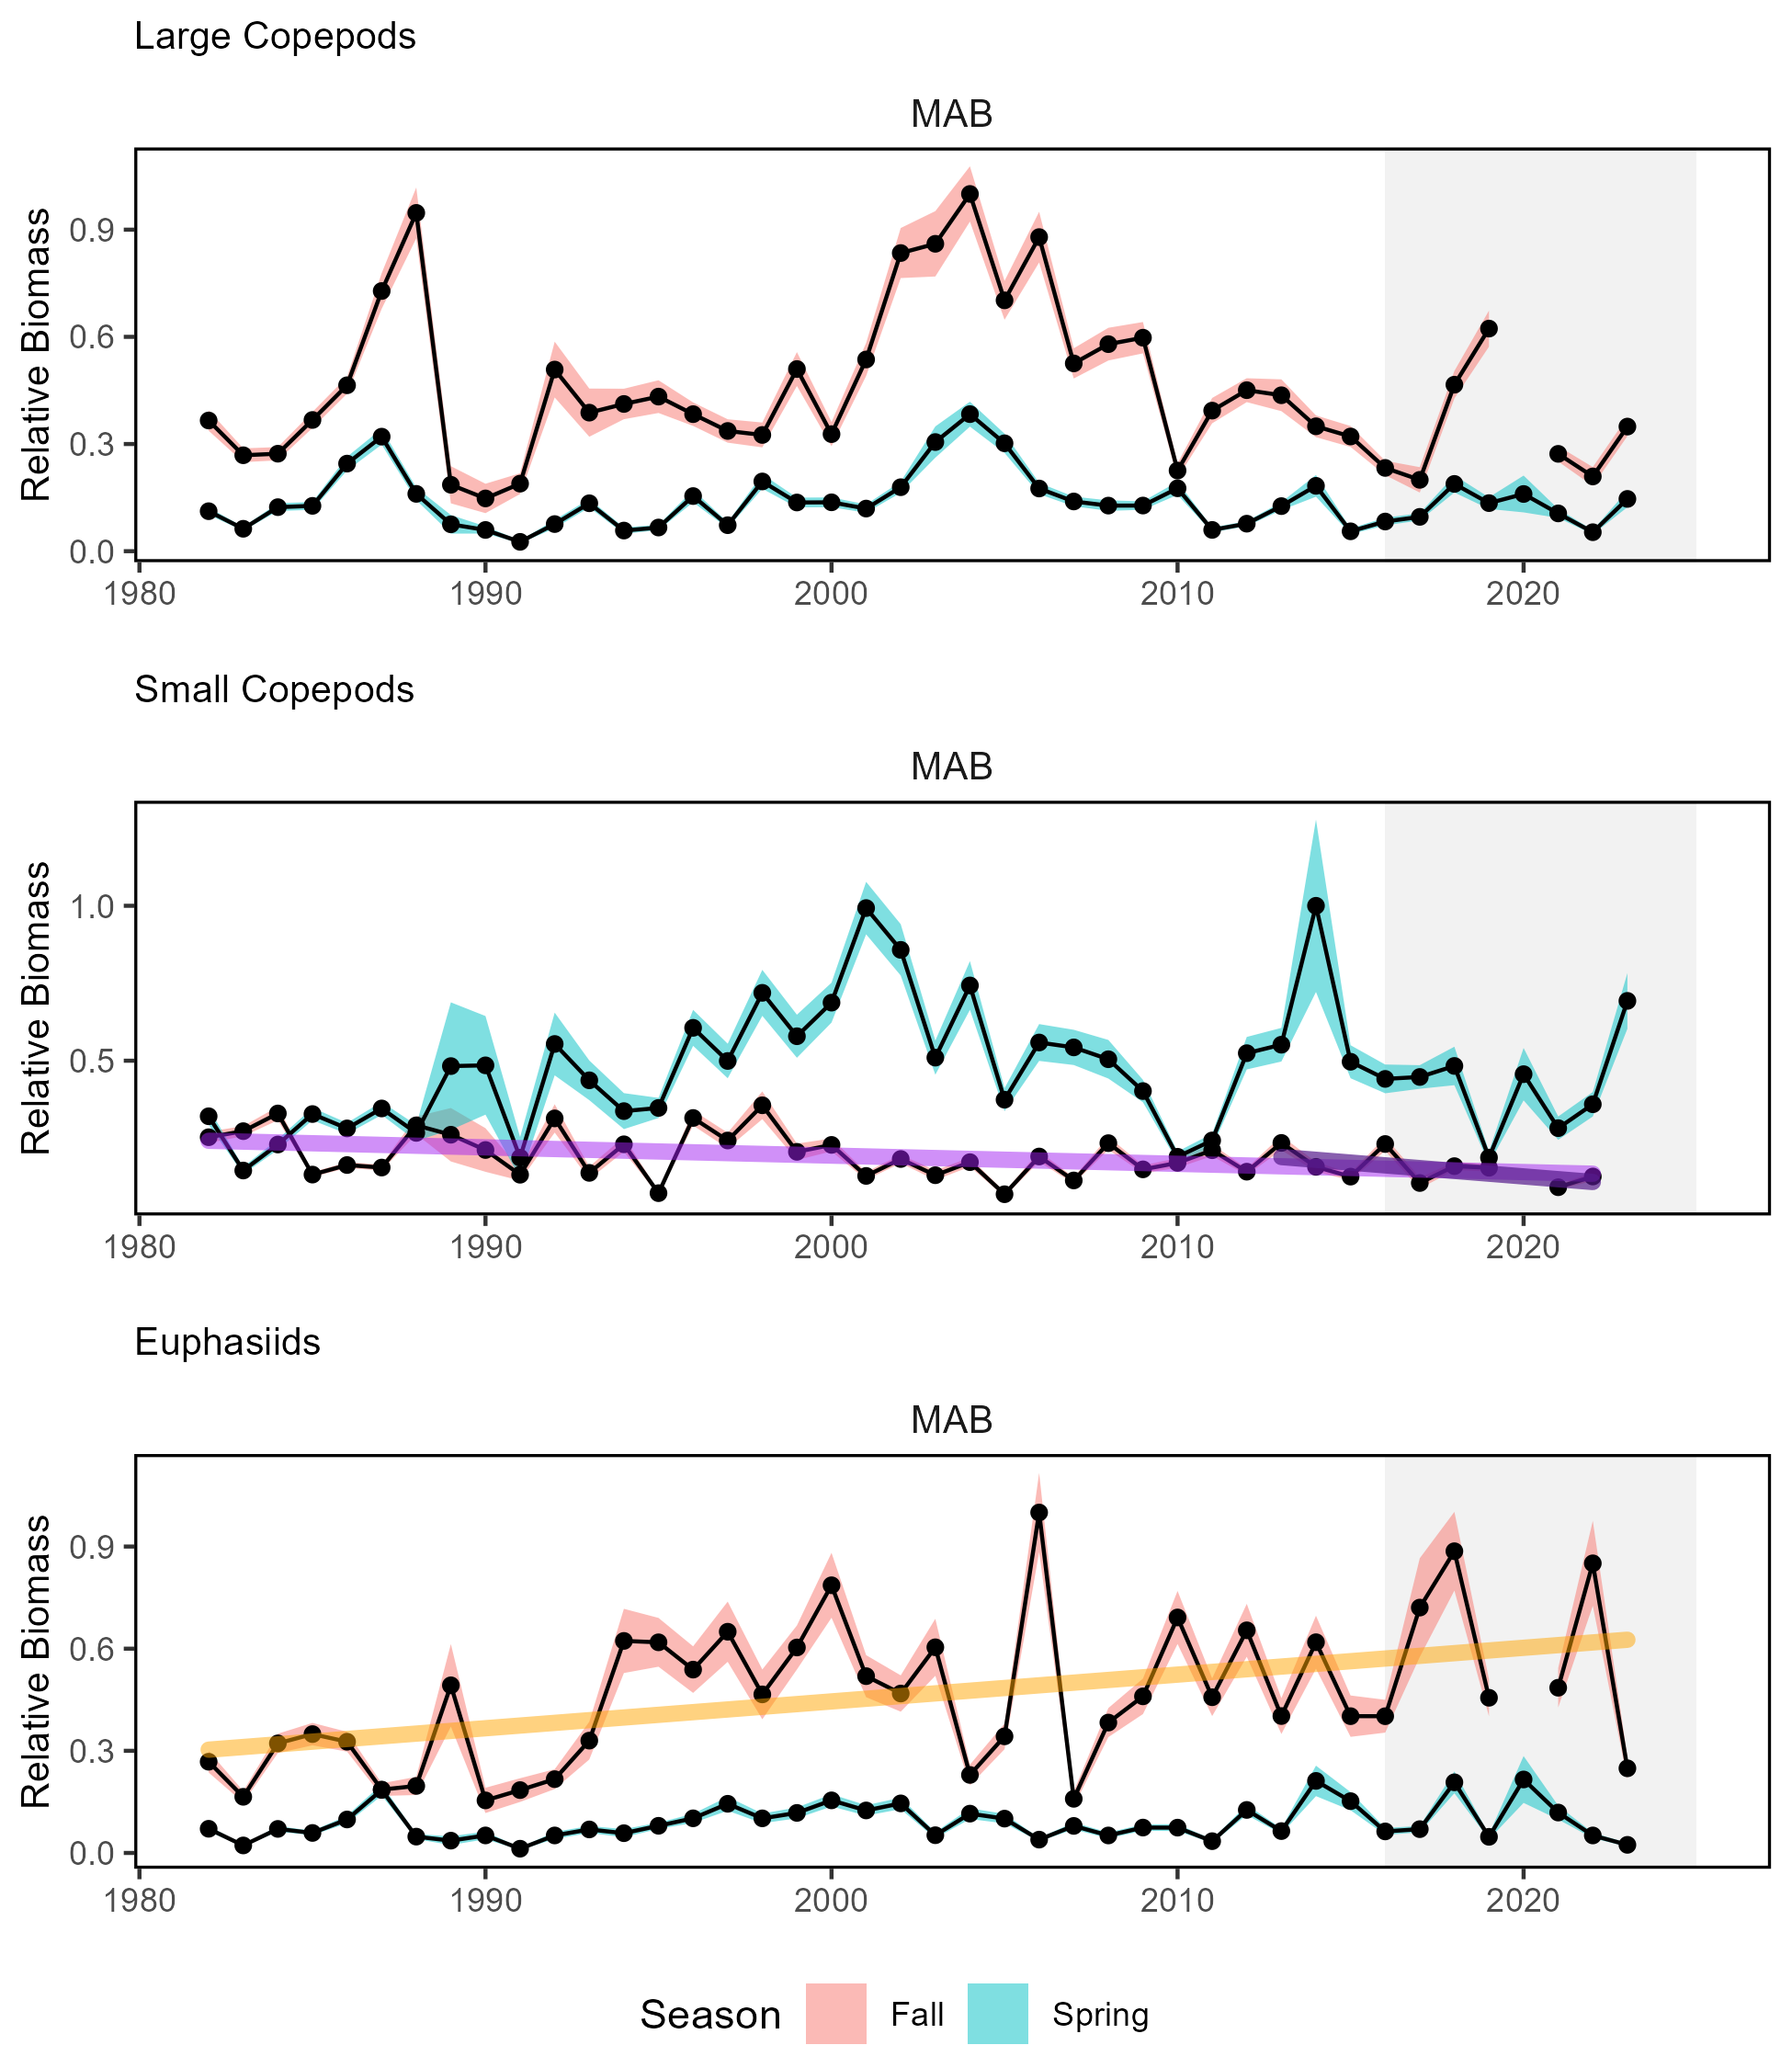
\includegraphics[width=1\linewidth,]{images/MidAtlantic/zooplankton_anomaly_MidAtlantic_2026-03-26} 

}

\caption{Changes in the abundance anomalies of three zooplankton groups in the Mid-Atlantic Bight: large copepods (includes \textit{Calanus finmarchicus}, top), small copepods (including \textit{C. typicus} and \textit{Pseudocalanus spp.}), and Euphausiids (bottom), with significant decreases (short-term, dark purple; long-term, light purple) in small copepods and long-term increases (orange) in Euphausiids.}\label{fig:zoopanom}
\end{figure}

\subparagraph{Environmental Drivers}\label{environmental-drivers}

Fish production can also be directly related to the prevailing environmental conditions by altering metabolism (growth), reproductive processes, and survival. Marine species possess thermal tolerances and can experience stressful or lethal conditions if water temperatures exceed certain levels. We have observed in past years extreme temperatures at both the \href{https://noaa-edab.github.io/catalog/seasonal_oisst_anom.html}{surface} and \href{https://noaa-edab.github.io/catalog/bottom_temp_model_anom.html}{bottom} that exceed \href{https://noaa-edab.github.io/catalog/thermal_habitat_gridded.html}{thermal tolerance} limits for some fish and shellfish. However, in 2025, Mid-Atlantic surface and bottom temperatures were near or below the long-term average and the amount of habitat exceeding a 24°C thermal tolerance was limited to the southern MAB, where those conditions occurred for fewer than 30 days (Fig. \ref{fig:therm-hab-persist-2024}).

A single surface \href{https://noaa-edab.github.io/catalog/heatwave.html}{marine heatwave} occurred in the Mid-Atlantic Bight in 2025, starting July 15th and lasting seven days. This brief event was the only heatwave recorded across the entire Continental Shelf for the year. The MAB experienced six surface marine \href{https://noaa-edab.github.io/catalog/cold_spell.html}{cold spells} in 2025 (Fig. \ref{fig:mcs-bottom-mab}), including an event in February that ranked as the 8th strongest on record. Additionally, a significant bottom cold spell occurred in January, lasting 57 days and ranking as the 5th strongest on record. During this period, bottom temperatures averaged 7.2°C, nearly 2°C lower than the historical average.

Lower ocean temperatures near long-term averages will affect species differently across the region. While cold-water species like cod may benefit from these conditions, warm-water species such as black sea bass are unlikely to see positive effects. This variability in regional cooling highlights the need for management to account for shifting species distributions and productivity.

\begin{figure}[T]

{\centering 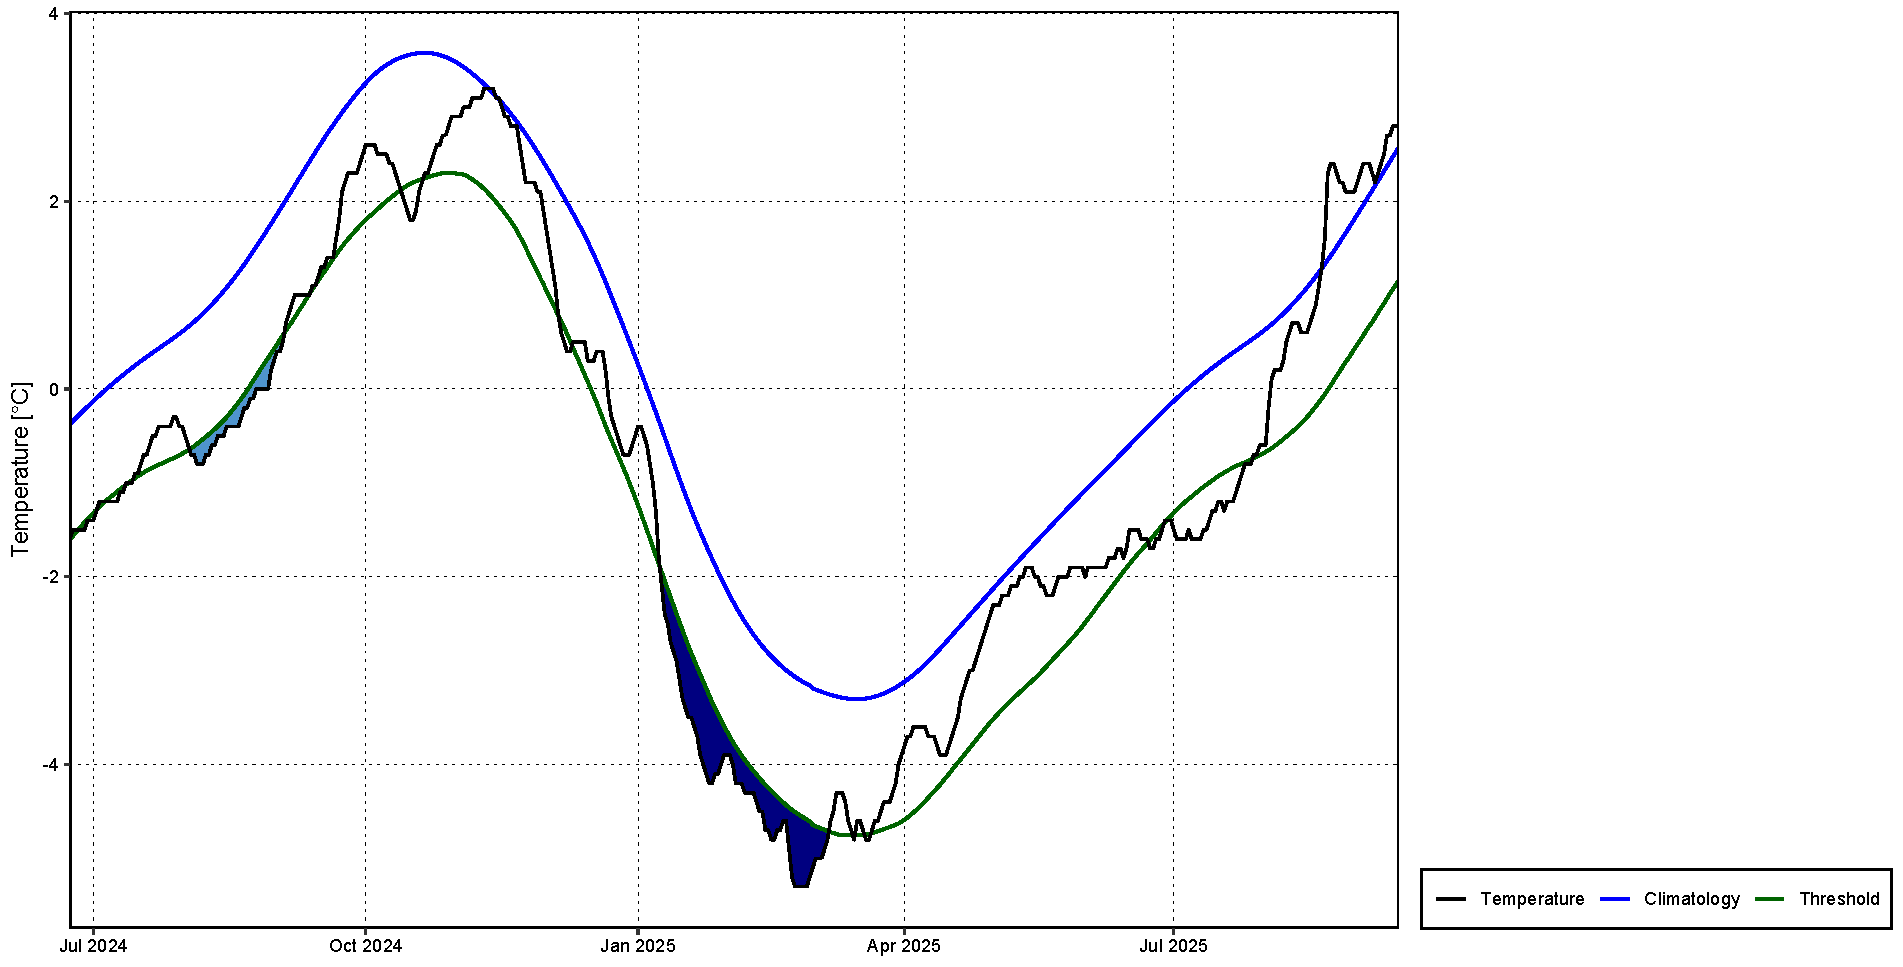
\includegraphics[width=1\linewidth,]{images/MidAtlantic/SOE_2026_MAB_Bottom_MCS} 

}

\caption{Marine cold spells based on detrended GLORYS12V1 bottom temperature from July 2024 though December 2025 in the MAB. Cold spells defined by events where observered temperature (black) exceeds  a threshold (green) based on the climatology (blue). Blue shaded areas show the cold spell events with the largest event in dark blue. }\label{fig:mcs-bottom-mab}
\end{figure}

\begin{figure}[T]

{\centering 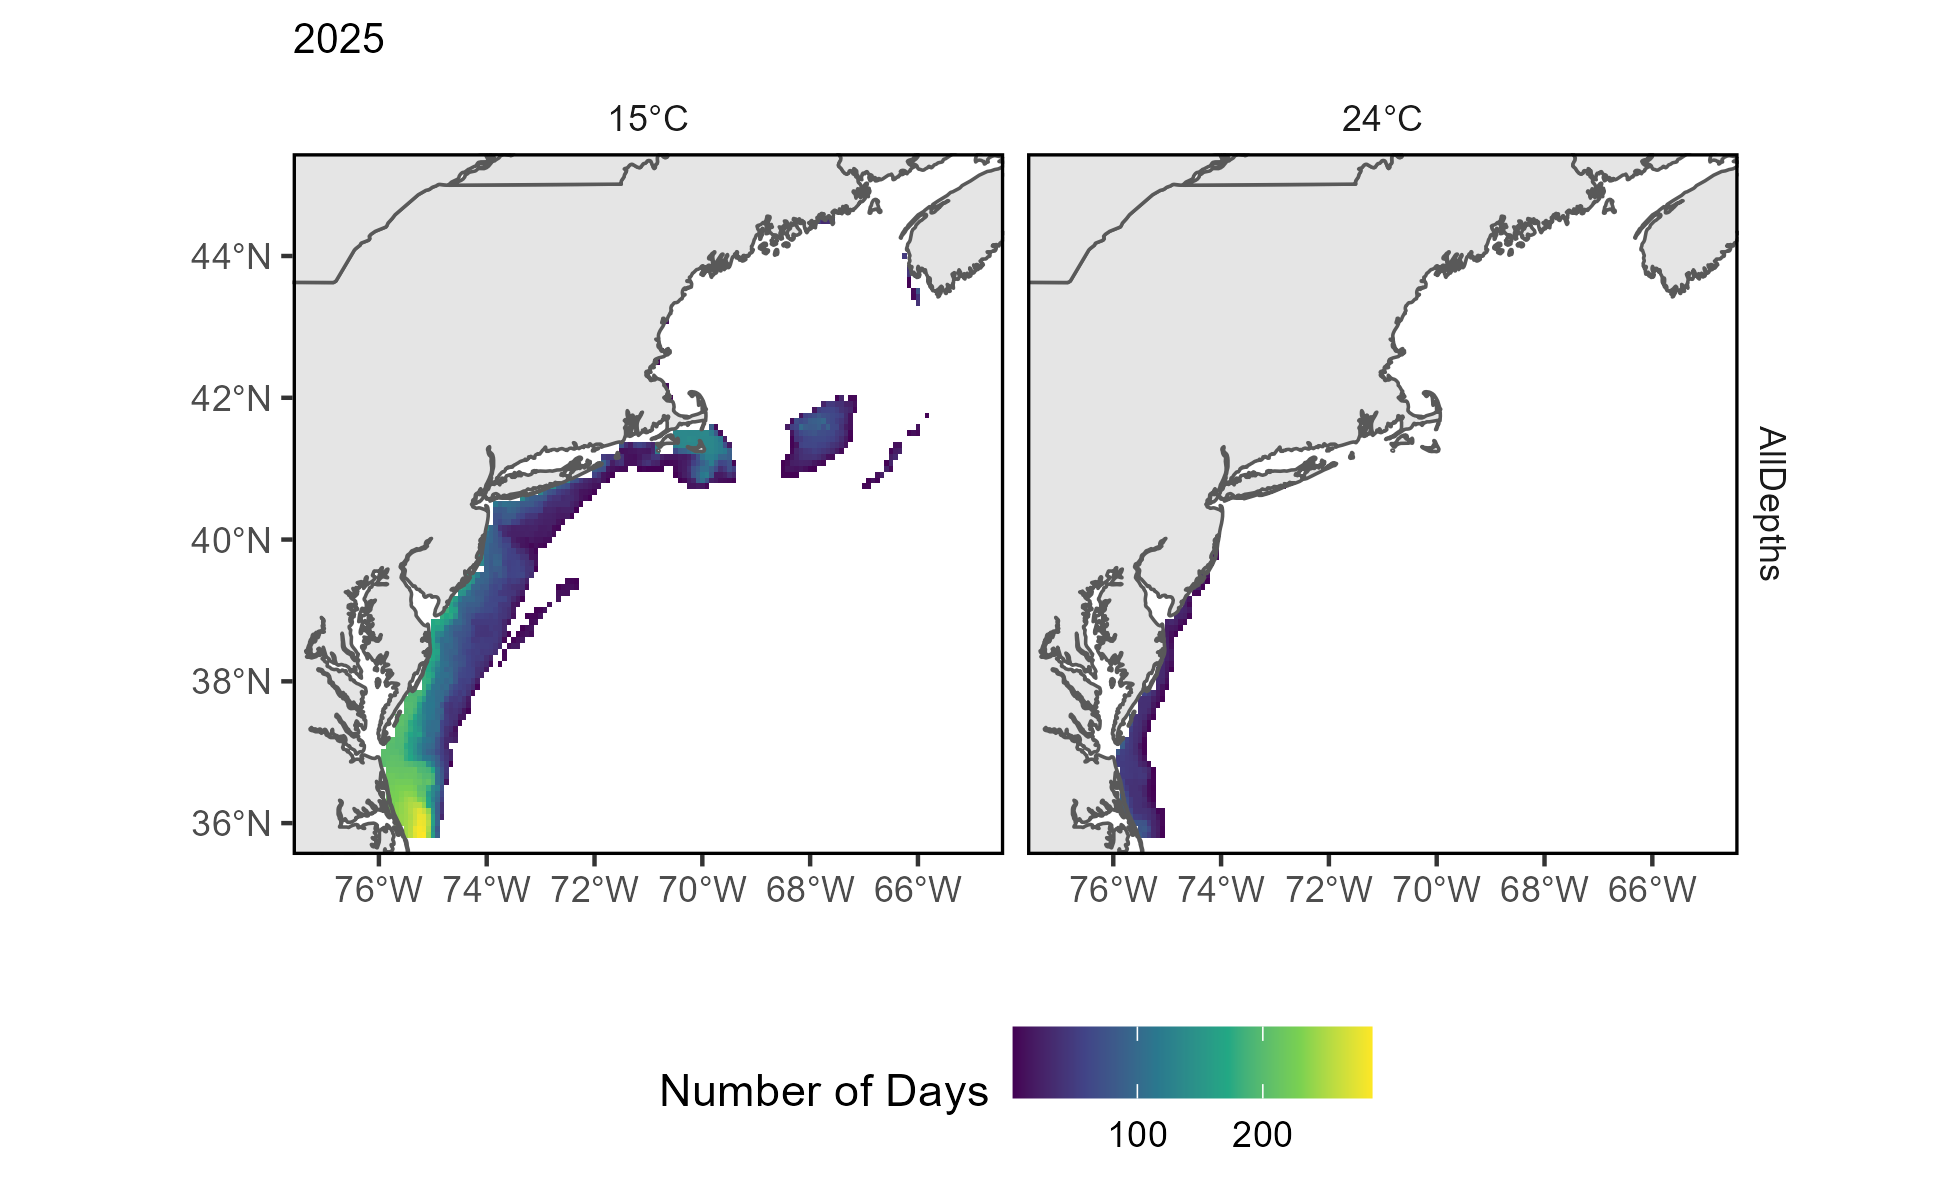
\includegraphics[width=1\linewidth,]{images/BothReports/therm_hab_persist_BothReports_2026-02-02} 

}

\caption{The number of days in 2025 where bottom temperature exceeds 15 degrees (left) and 24 degrees (right) based on the GLORYS 1/12 degree grid.}\label{fig:therm-hab-persist-2024}
\end{figure}

The newly-developed \href{https://noaa-edab.github.io/catalog/advection.html}{advection index} (Fig. \ref{fig:advection-index}) shows total transport of water onto and off the continental shelf which can impact the survival of early life stages of fish and invertebrates. Long-term trends in the Mid-Atlantic show increased offshore movement of surface and bottom waters in June, which could decrease retention of some species. Further species level studies are needed to link spawning timing and larval periods to advection trends at the corresponding spatial and temporal scales, depth, and month.

\begin{figure}[T]

{\centering 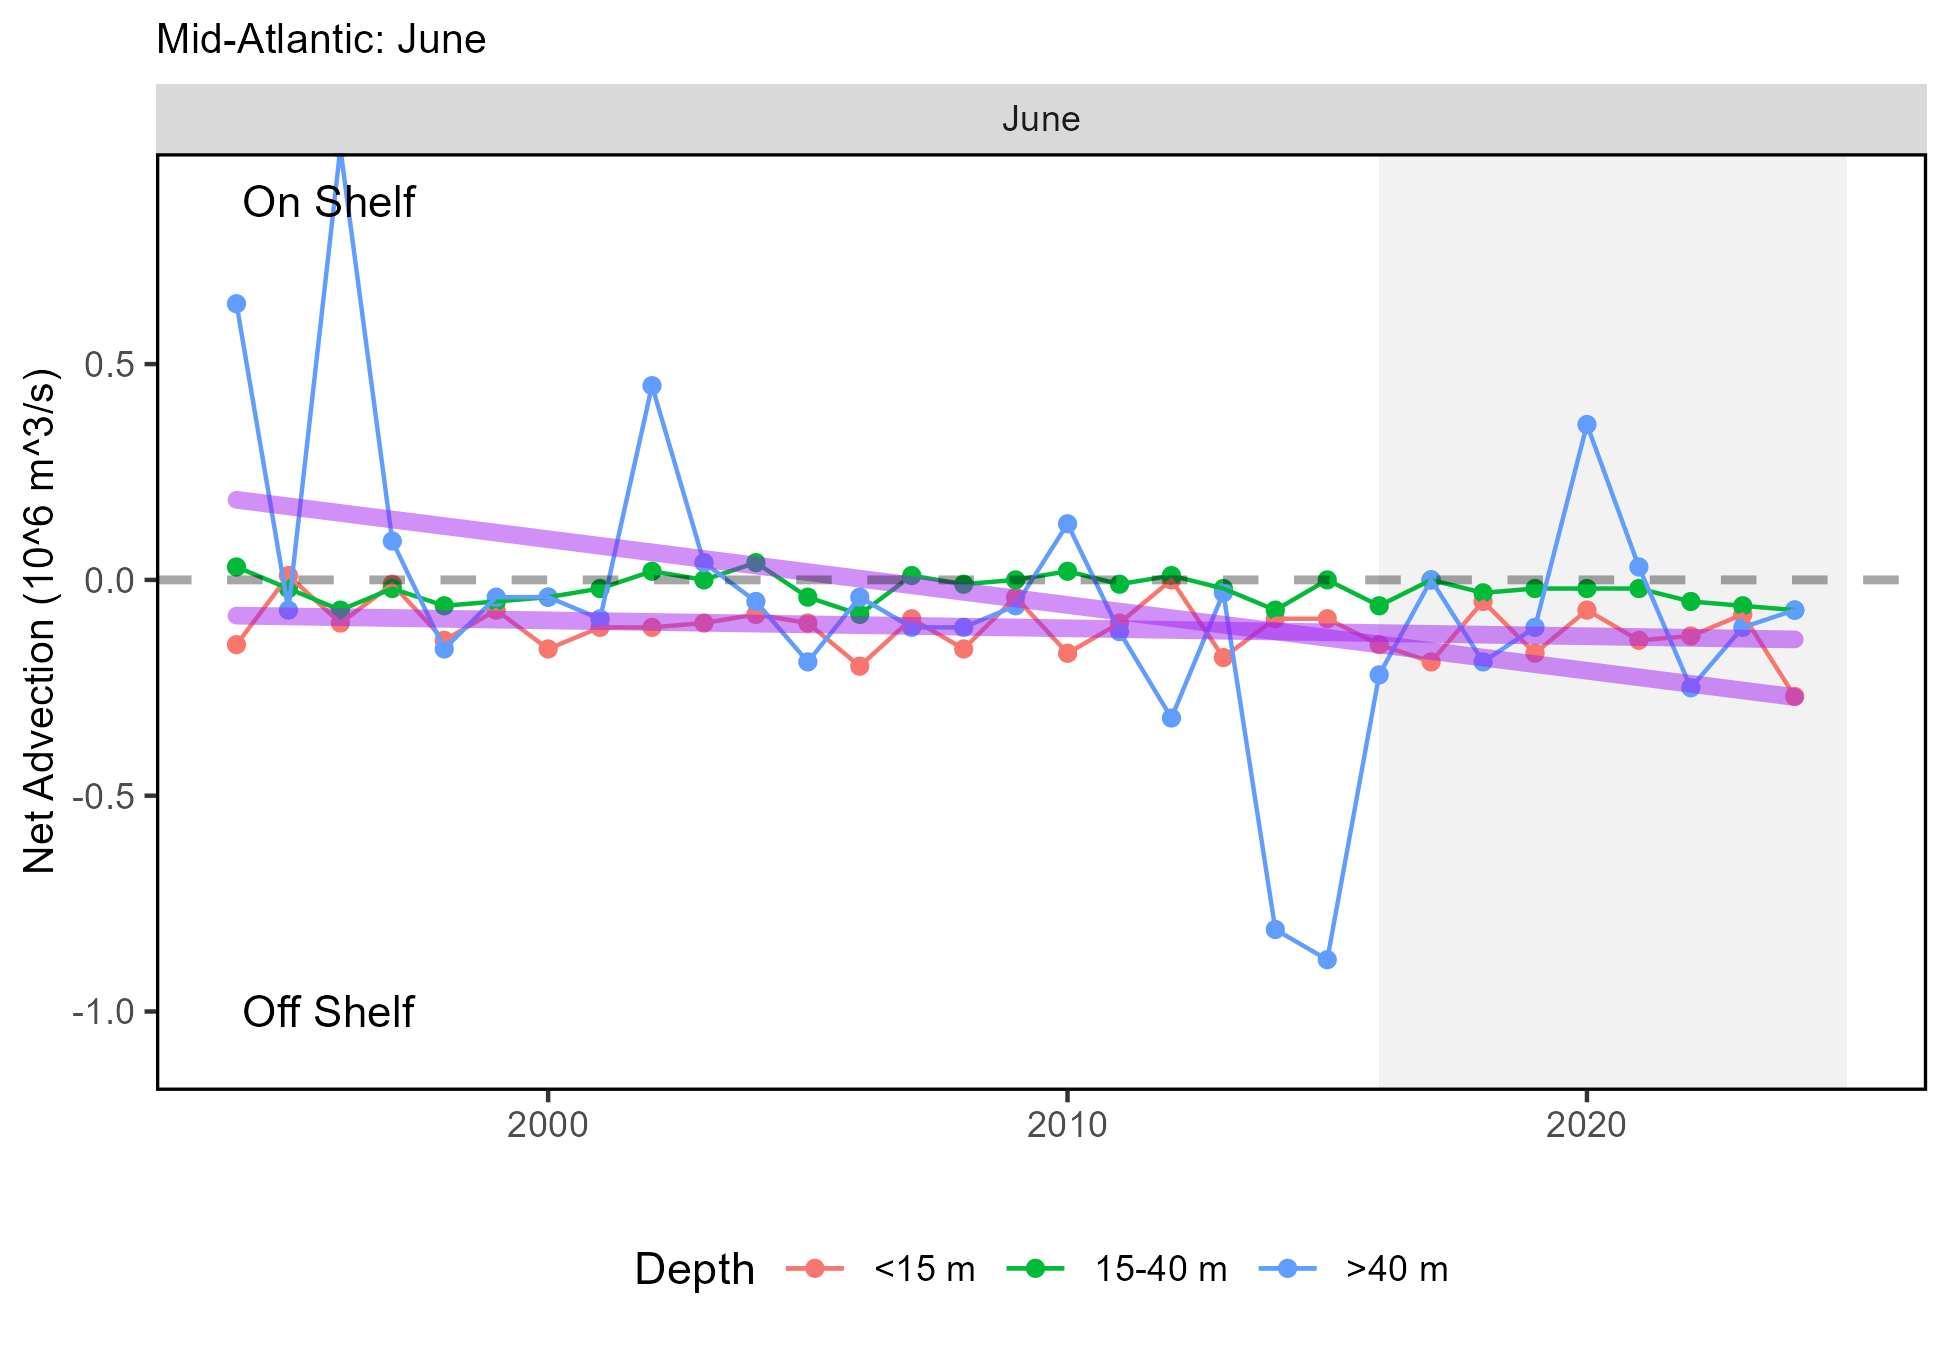
\includegraphics[width=1\linewidth,]{images/MidAtlantic/advection_index_MidAtlantic_2026-03-26} 

}

\caption{Net advection in June across the Mid-Atlantic continental shelf break within 3 depth bands, with significant long-term declines (purple) in >40m and <15m. }\label{fig:advection-index}
\end{figure}

\href{https://noaa-edab.github.io/catalog/ocean_acidification.html}{Ocean acidification} (OA) risks vary among species and include reduced survival, growth, reproduction, and productivity, where high OA risk indicates potential negative effects to species. OA risk can also be heightened during colder conditions due to increased CO2 absorption by colder water or by transport of high CO2 water masses as was suggested to have occurred in 2024 (see \href{https://noaa-edab.github.io/catalog/observation_synthesis_2024.html}{2024 Highlights}). The OA indicator observed on the Mid-Atlantic coastal shelf during summer 2024 was the most extreme recorded when compared to all of the years sampled (since 2007). In 2025, however, OA risk conditions were less than those observed in 2023 and 2024. High OA conditions in 2025 were limited to a few outer shelf coastal New Jersey (NJ) observations in spring, where sensitivity levels for Atlantic sea scallops were exceeded (not shown, see \href{https://noaa-edab.github.io/catalog/ocean_acidification.html}{ocean acidification}), and in nearshore NJ waters in summer, where sensitivity levels for Longfin squid were reached (Fig. \ref{fig:mab-oa}). Although relatively cool bottom seawater temperatures in 2025 were similar to 2024, salinity was higher in 2025, which suggests a different composition of oceanographic properties and water masses between the two years and as a result, different OA risk conditions.

\begin{figure}[T]

{\centering 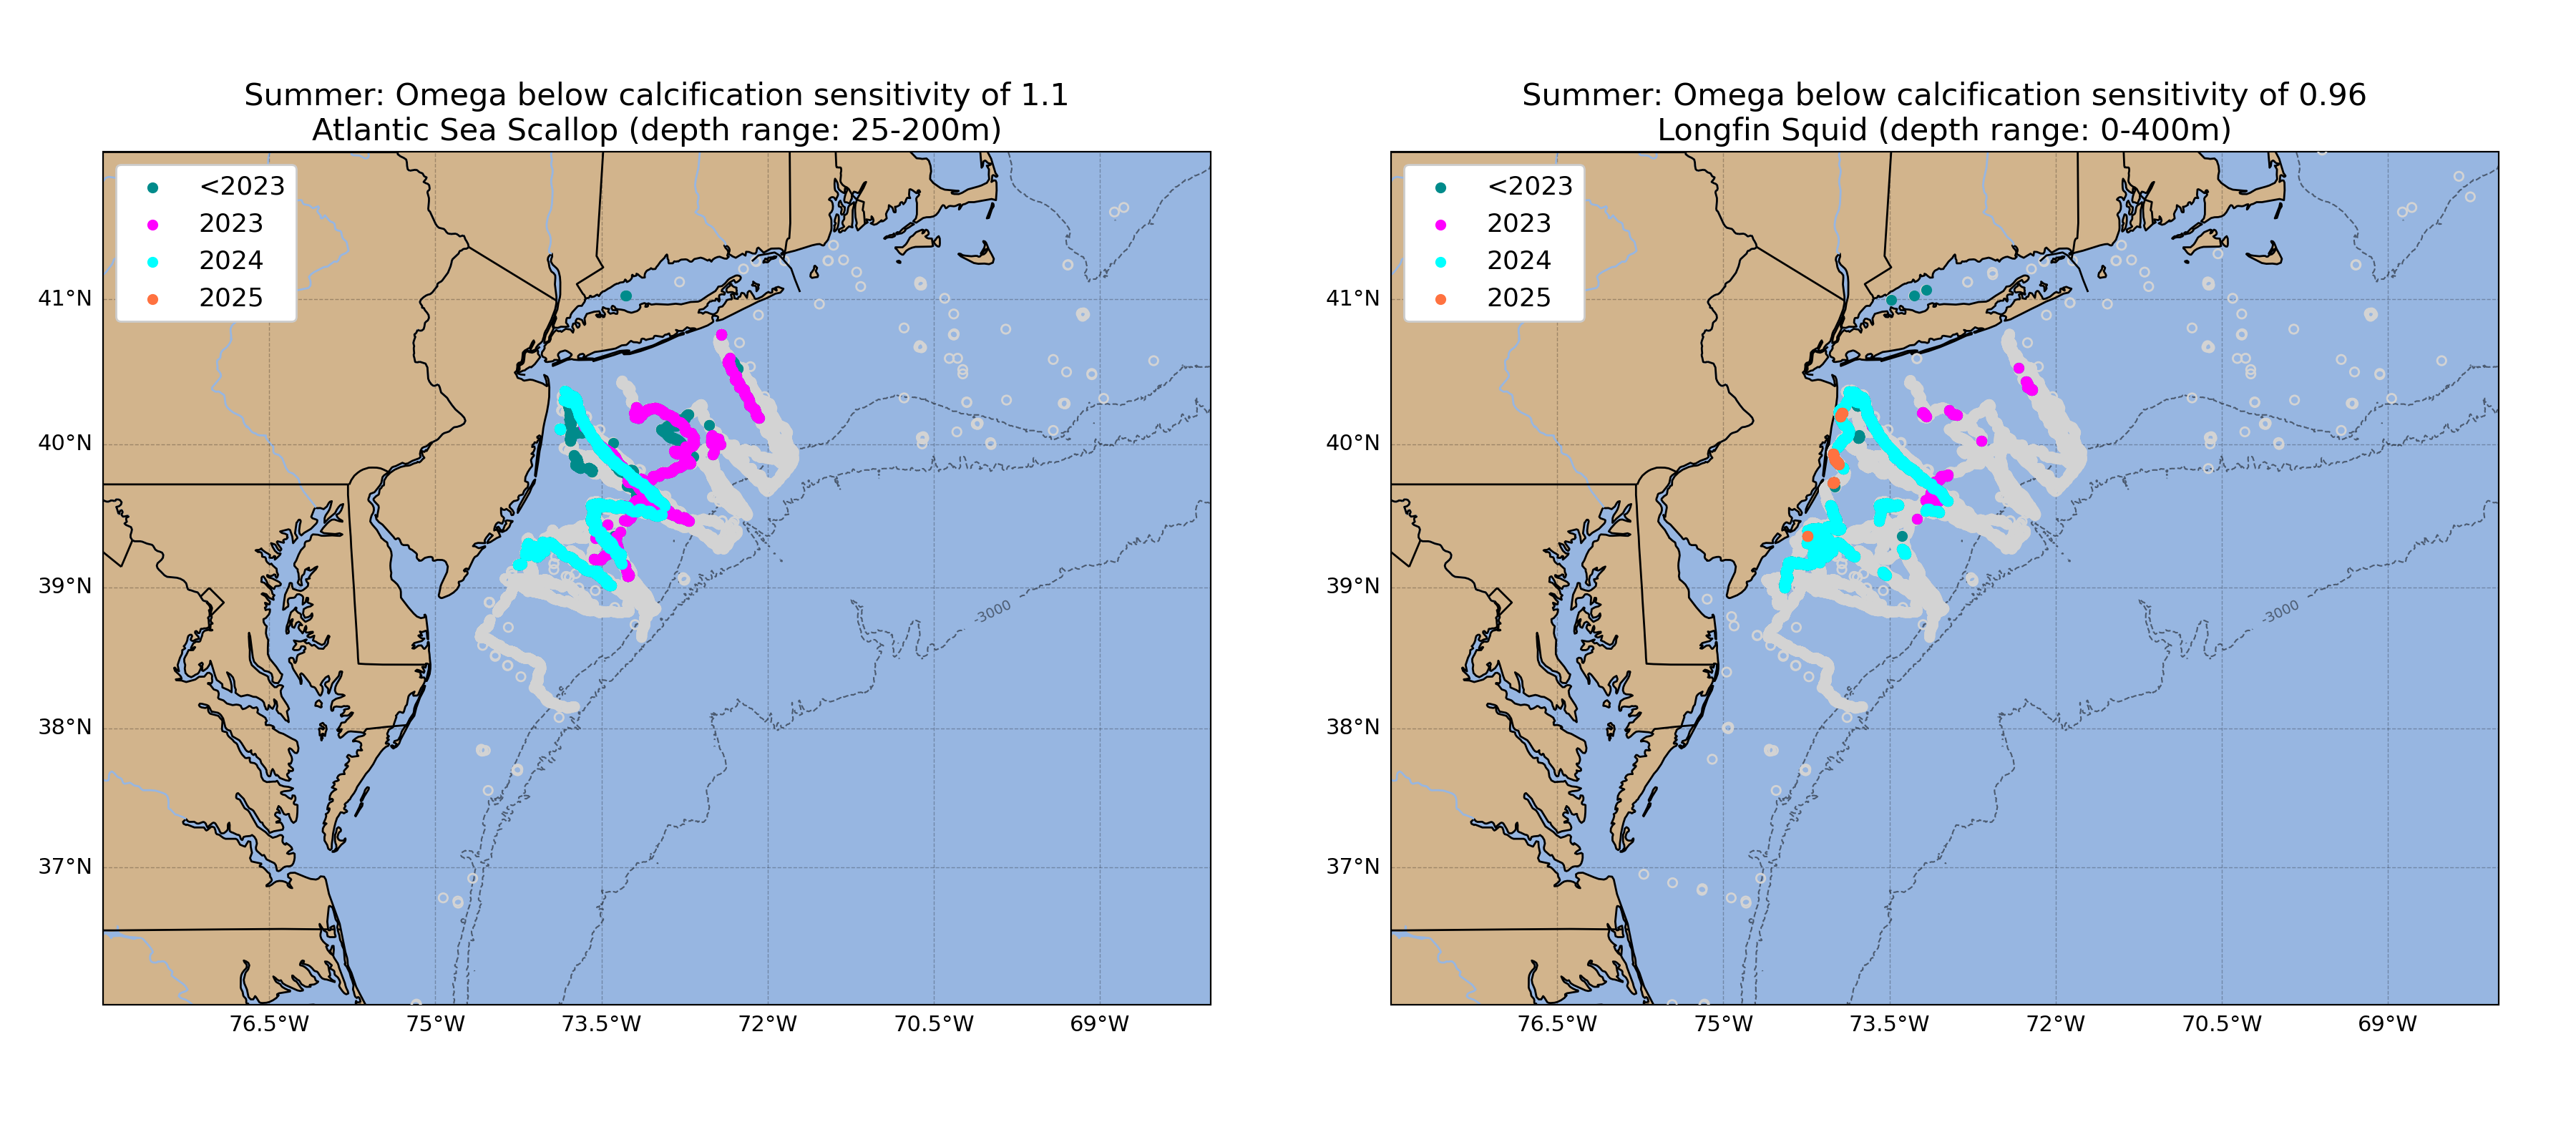
\includegraphics[width=1\linewidth,]{images/BothReports/final_bottom_omega_2026} 

}

\caption{Locations where bottom aragonite saturation state ($\Omega_{Arag}$; summer only: June-August) were at or below the laboratory-derived sensitivity level for Atlantic sea scallop (left panel) and longfin squid (right panel) for the time periods 2007-2022 (dark cyan), 2023 only (magenta) and 2024 only (cyan). Gray circles indicate locations where bottom $\Omega_{Arag}$ values were above the species specific sensitivity values.}\label{fig:mab-oa}
\end{figure}

`

\href{https://noaa-edab.github.io/catalog/dissolved_oxygen.html}{Low dissolved oxygen levels} (\textless{} 5 mg/L) remained localized and brief on the \href{https://noaa-edab.github.io/catalog/observation_synthesis_2023.html}{MAB shelf in 2025}, resulting in no industry-reported mass mortality events despite the potential for hypoxia to reduce species growth or cause death. Localized hypoxia (\textless{} 2 mg/L) occurred nearshore east of Point Pleasant, NJ, southwest of Newport, RI, and at the western end of the Cape Cod Canal, while broader shelf-wide levels below 5 mg/L were not widespread. This contrast follows previous years where \href{https://noaa-edab.github.io/catalog/observation_synthesis_2023.html}{hypoxic} events in Cape Cod Bay (2019, 2020) and off New Jersey (2023) potentially caused fish, lobster, and crab \href{https://sebsnjaesnews.rutgers.edu/2023/12/rutgers-scientists-observe-unusual-ocean-conditions-possibly-linked-to-mortality-in-marine-life-off-new-jersey/}{mortality}. While shelf-wide monitoring data is currently limited, biological and oceanographic drivers of oxygen levels continue to be tracked to assess the duration and extent of future events.

\subparagraph{Drivers: Predation}\label{drivers-predation}

The abundance and distribution of marine mammal, shark , and other Atlantic Highly Migratory Species (HMS) predators, can affect both the productivity and mortality rates on managed stocks. Predators can consume managed species or compete for the same resources, resulting in increased natural mortality or decreased productivity. The northeast shift in \href{https://noaa-edab.github.io/catalog/cetacean_dist.html}{whales and dolphins} (Fig. \ref{fig:protectedspp-dist-shifts}) indicates a change in the overlap between marine mammals and managed fishes. Managed fishes also act as predators on other managed species. Since we also observe distribution shifts in managed species as well as forage species, the effect of changing predator distributions alone is difficult to quantify.

Indicators for shark populations, combined with information on gray seals (see \hyperref[protected-species]{Protected Species Implications section, above}), suggests predator populations range from stable (\href{https://noaa-edab.github.io/catalog/hms_cpue.html}{sharks}) to increasing (\href{https://noaa-edab.github.io/catalog/seal_pups.html}{gray seals}) in the MAB. \href{https://noaa-edab.github.io/catalog/hms_stock_status.html}{Stock status} is mixed for HMS stocks (including sharks, swordfish, billfish, and tunas) occurring throughout the Northeast U.S. shelf. While there are several HMS species considered to be overfished or that have unknown stock status, the population status for some managed Atlantic sharks and tunas is at or above the biomass target, suggesting the potential for robust (or rebuilt) predator populations and subsequent predation pressure on managed species. Increasing predator populations or changing distribution of predators may result in increased predation pressure.

\paragraph{Future Considerations}\label{future-considerations-2}

The processes that control fish productivity and mortality are dynamic, complex, and the result of the interactions between multiple system drivers. Fishing effects could impact fish productivity, although we do not explore those connections at this time. There is a real risk that short-term predictions in assessments and rebuilding plans that assume unchanging underlying conditions will not be as effective, given the observed ecological and environmental process changes documented throughout the report. Assumptions for species' growth, reproduction, and natural mortality should continue to be evaluated for individual species. With observations of system-wide productivity shifts of multiple managed stocks, more research is needed to determine whether regime shifts or ecosystem reorganization are occurring, and how this should be incorporated into management.

\subsection{Other Ocean Uses: Offshore Wind}\label{other-ocean-uses-offshore-wind}

Offshore wind development is active and dynamic throughout the region. The following section reflects the status of projects as of the end of January 2026.

\subsubsection{Indicators: development timeline, revenue in lease areas, coastal community vulnerability}\label{indicators-development-timeline-revenue-in-lease-areas-coastal-community-vulnerability}

Offshore wind indicators are used to quantify the influence of offshore wind on fisheries and ecosystems. They are based on BOEM's Offshore Renewable Activities page and projects' Final Environmental Impact Statements. In 2025, Presidential Memorandum 90 FR 8363 removed existing planning areas and excluded the establishment of additional lease areas.

As of January 2026, 38 offshore \href{https://noaa-edab.github.io/catalog/wind_dev_speed.html}{wind development} leases are under different stages of development in the Northeast (Fig. \ref{fig:wind-dev-cumul}). One project (South Fork Wind Farm) is fully operational and another (Vineyard Wind 1) is partially operational while construction finishes. The southern New England region has two other projects currently under construction (Revolution Wind and Sunrise Wind). Empire Wind and Coastal Virginia Offshore Wind (CVOW) are currently under construction in the New York Bight and Mid-Atlantic Region, respectively, with CVOW expected to start generating power in early 2026.

Construction of these projects during 2025 affected fisheries managed by the Mid-Atlantic Fishery Management Council. There are eight additional projects that have Construction and Operations Plan (COP) approvals (three in Southern New England and five in the Mid-Atlantic/New York Bight) that could begin construction in 2026, however, construction schedules are highly uncertain at this time. Seven additional projects have submitted COPs and are pending approval, while the remaining projects are under the site assessment phase and have not submitted COPs to date (Fig. \ref{fig:wind-dev-cumul}).

With the first offshore wind energy projects now under construction and operation, all indicator analyses in this section follow a different reporting format than in previous years. Where previous years reported data for all lease areas, this year we investigate impacts of the six commercial scale projects currently under construction or operation, (i.e., Active Projects: South Fork Wind Farm, Revolution Wind, Sunrise Wind, Empire Wind 1, Vineyard Wind 1, and CVOW-Commercial).

\begin{figure}[T]

{\centering 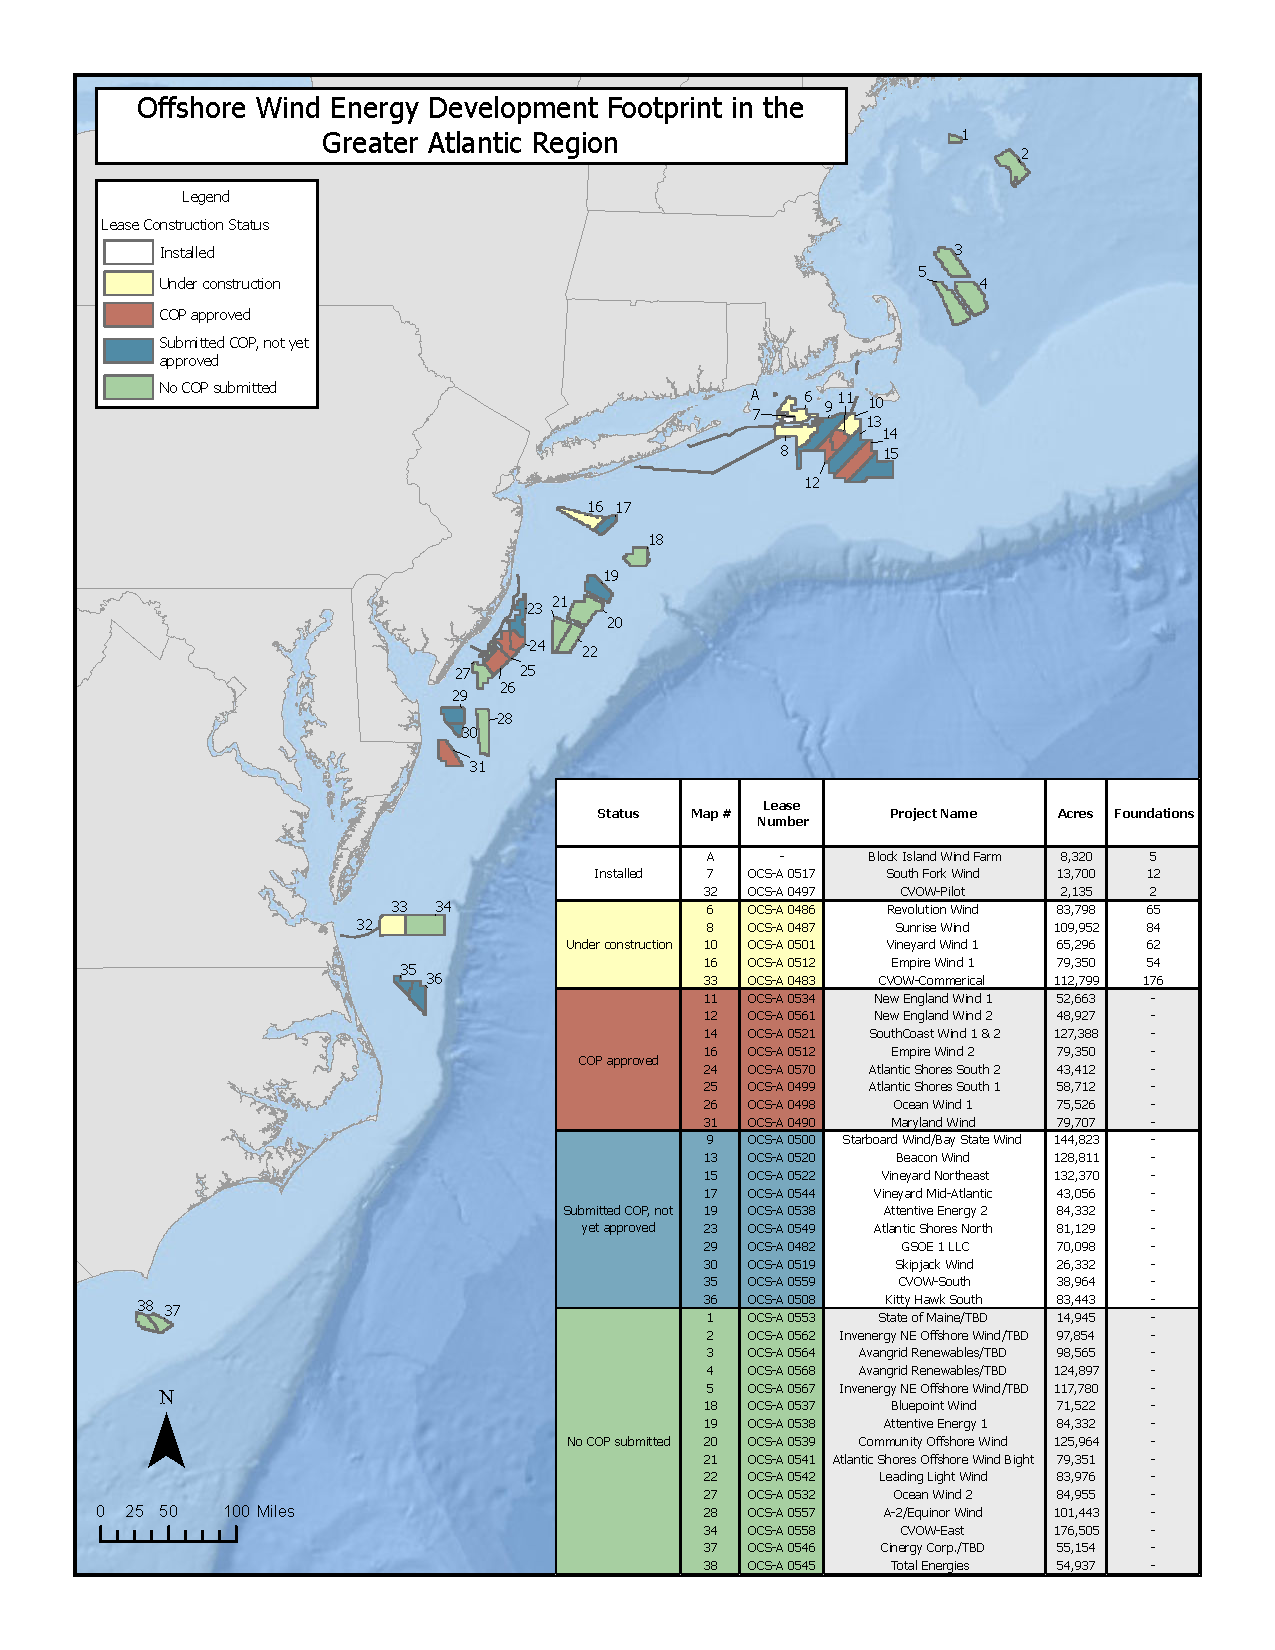
\includegraphics[width=0.9\linewidth,]{images/BothReports/OffshoreWindDevelopmentMap_V3_NicoleMucci} 

}

\caption{All Northeast wind energy lease areas, colored by lease construction status.}\label{fig:wind-dev-cumul}
\end{figure}

Offshore wind indicators are based on federal logbook data and do not include all data for all fisheries; therefore a complete evaluation of potential offshore wind energy development impacts would need to be supplemented by other data sources. For further information on the utility of the data, see the \href{https://www.fisheries.noaa.gov/resource/data/socioeconomic-impacts-atlantic-offshore-wind-development}{socioeconomic impacts of offshore wind development data reports page}.

\href{https://noaa-edab.github.io/catalog/wind_revenue.html}{Commercial fishery revenue} from trips within Active Projects have varied annually from 2008-2024, with less than \$500,000 in maximum annual revenue overlapping with these areas for most fisheries with the exception of longfin squid (\$2 million), monkfish (\$1.1 million), ocean quahog (\$783,000), and summer flounder (\$556,000) in specific years (Fig. \ref{fig:wea-spp-rev}).

\begin{figure}[T]

{\centering 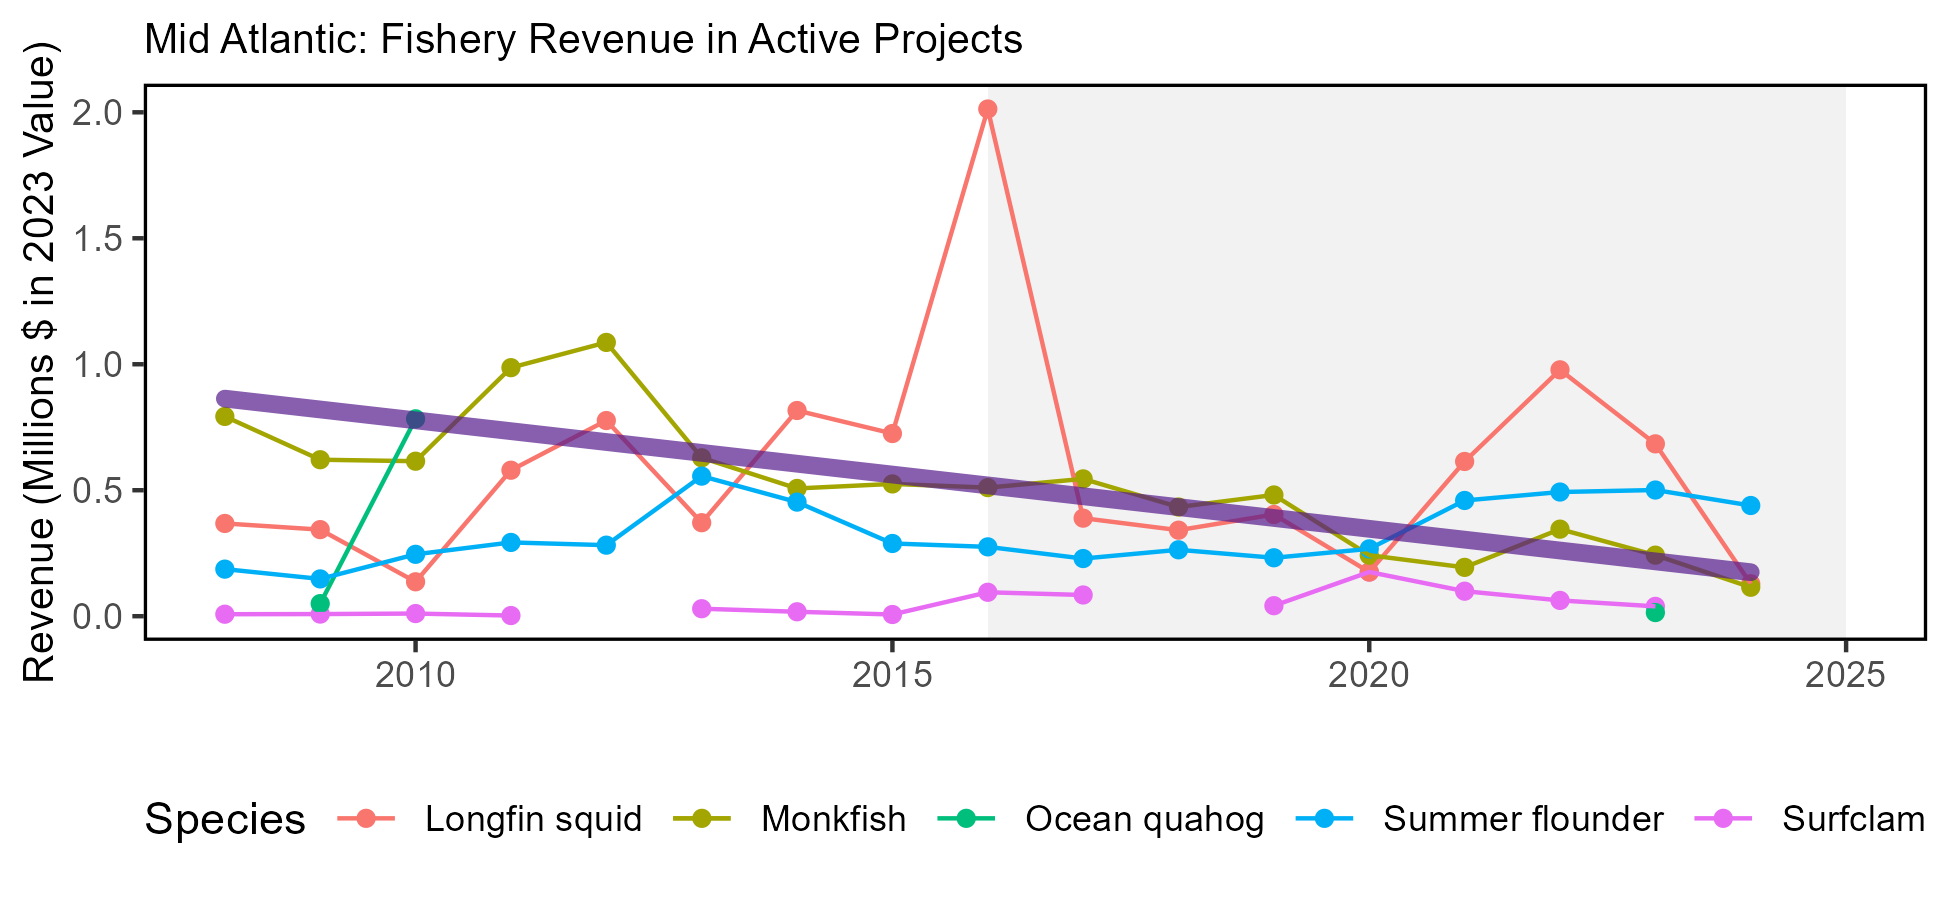
\includegraphics[width=1\linewidth,]{images/MidAtlantic/wind_revenue_MidAtlantic_2026-03-26} 

}

\caption{Revenue of species managed by the Mid-Atlantic Fishery Management Council within Active Projects. The declining trendline (purple) is associated with monkfish. }\label{fig:wea-spp-rev}
\end{figure}

Based on revenue between 2008-2024, MAFMC-managed fisheries derived a maximum of 6\% of annual regional fishery revenue from the Active Project areas. The specific fisheries affected include chub mackerel (6\% of revenue), bluefish (5\%), butterfish (4\%), and monkfish, scup, black sea bass, and longfin squid (3\% each) (Table \ref{tab:wea-landings-rev}). Future offshore wind development may increase effects on these and additional species if more projects begin construction. Future fishery resource overlap with wind leases, especially surfclams and ocean quahogs, may change due to species distribution shifts attributable to climate change and recruitment and larval dispersion pattern changes caused by hydrodynamic flow disruptions from turbine foundations, which could also affect fishery landings and/or revenue.

\global\setlength{\Oldarrayrulewidth}{\arrayrulewidth}

\global\setlength{\Oldtabcolsep}{\tabcolsep}

\setlength{\tabcolsep}{2pt}

\renewcommand*{\arraystretch}{1}



\providecommand{\ascline}[3]{\noalign{\global\arrayrulewidth #1}\arrayrulecolor[HTML]{#2}\cline{#3}}

\begin{longtable}[c]{|p{2.00in}|p{2.00in}|p{2.00in}}

\caption{Top\ 10\ Mid-Atlantic\ managed\ species\ landings\ and\ revenue\ from\ Active\ Projects.\ *These\ species\ did\ not\ have\ more\ than\ 50,000\ lbs\ landed\ from\ the\ Active\ Project\ areas\ in\ any\ year.}\label{tab:wea-landings-rev}\\

\ascline{1.5pt}{666666}{1-3}

\multicolumn{1}{>{\raggedright}m{\dimexpr 2in+0\tabcolsep}}{\textcolor[HTML]{000000}{\fontsize{9}{9}\selectfont{NEFMC,\ MAFMC,\ and\ ASMFC\ Managed\ Species}}} & \multicolumn{1}{>{\raggedleft}m{\dimexpr 2in+0\tabcolsep}}{\textcolor[HTML]{000000}{\fontsize{9}{9}\selectfont{Maximum\ Percent\ Total\ Annual\ Regional\ Species\ Landings}}} & \multicolumn{1}{>{\raggedleft}m{\dimexpr 2in+0\tabcolsep}}{\textcolor[HTML]{000000}{\fontsize{9}{9}\selectfont{Maximum\ Percent\ Total\ Annual\ Regional\ Species\ Revenue}}} \\

\ascline{1.5pt}{666666}{1-3}\endfirsthead \caption[]{Top\ 10\ Mid-Atlantic\ managed\ species\ landings\ and\ revenue\ from\ Active\ Projects.\ *These\ species\ did\ not\ have\ more\ than\ 50,000\ lbs\ landed\ from\ the\ Active\ Project\ areas\ in\ any\ year.}\label{tab:wea-landings-rev}\\

\ascline{1.5pt}{666666}{1-3}

\multicolumn{1}{>{\raggedright}m{\dimexpr 2in+0\tabcolsep}}{\textcolor[HTML]{000000}{\fontsize{9}{9}\selectfont{NEFMC,\ MAFMC,\ and\ ASMFC\ Managed\ Species}}} & \multicolumn{1}{>{\raggedleft}m{\dimexpr 2in+0\tabcolsep}}{\textcolor[HTML]{000000}{\fontsize{9}{9}\selectfont{Maximum\ Percent\ Total\ Annual\ Regional\ Species\ Landings}}} & \multicolumn{1}{>{\raggedleft}m{\dimexpr 2in+0\tabcolsep}}{\textcolor[HTML]{000000}{\fontsize{9}{9}\selectfont{Maximum\ Percent\ Total\ Annual\ Regional\ Species\ Revenue}}} \\

\ascline{1.5pt}{666666}{1-3}\endhead



\multicolumn{1}{>{\raggedright}m{\dimexpr 2in+0\tabcolsep}}{\textcolor[HTML]{000000}{\fontsize{9}{9}\selectfont{Chub\ Mackerel*}}} & \multicolumn{1}{>{\raggedleft}m{\dimexpr 2in+0\tabcolsep}}{\textcolor[HTML]{000000}{\fontsize{9}{9}\selectfont{5.32}}} & \multicolumn{1}{>{\raggedleft}m{\dimexpr 2in+0\tabcolsep}}{\textcolor[HTML]{000000}{\fontsize{9}{9}\selectfont{5.80}}} \\





\multicolumn{1}{>{\raggedright}m{\dimexpr 2in+0\tabcolsep}}{\textcolor[HTML]{000000}{\fontsize{9}{9}\selectfont{Bluefish*}}} & \multicolumn{1}{>{\raggedleft}m{\dimexpr 2in+0\tabcolsep}}{\textcolor[HTML]{000000}{\fontsize{9}{9}\selectfont{3.60}}} & \multicolumn{1}{>{\raggedleft}m{\dimexpr 2in+0\tabcolsep}}{\textcolor[HTML]{000000}{\fontsize{9}{9}\selectfont{4.85}}} \\





\multicolumn{1}{>{\raggedright}m{\dimexpr 2in+0\tabcolsep}}{\textcolor[HTML]{000000}{\fontsize{9}{9}\selectfont{Butterfish}}} & \multicolumn{1}{>{\raggedleft}m{\dimexpr 2in+0\tabcolsep}}{\textcolor[HTML]{000000}{\fontsize{9}{9}\selectfont{4.37}}} & \multicolumn{1}{>{\raggedleft}m{\dimexpr 2in+0\tabcolsep}}{\textcolor[HTML]{000000}{\fontsize{9}{9}\selectfont{3.88}}} \\





\multicolumn{1}{>{\raggedright}m{\dimexpr 2in+0\tabcolsep}}{\textcolor[HTML]{000000}{\fontsize{9}{9}\selectfont{Scup}}} & \multicolumn{1}{>{\raggedleft}m{\dimexpr 2in+0\tabcolsep}}{\textcolor[HTML]{000000}{\fontsize{9}{9}\selectfont{3.32}}} & \multicolumn{1}{>{\raggedleft}m{\dimexpr 2in+0\tabcolsep}}{\textcolor[HTML]{000000}{\fontsize{9}{9}\selectfont{3.26}}} \\





\multicolumn{1}{>{\raggedright}m{\dimexpr 2in+0\tabcolsep}}{\textcolor[HTML]{000000}{\fontsize{9}{9}\selectfont{Longfin\ Squid}}} & \multicolumn{1}{>{\raggedleft}m{\dimexpr 2in+0\tabcolsep}}{\textcolor[HTML]{000000}{\fontsize{9}{9}\selectfont{3.31}}} & \multicolumn{1}{>{\raggedleft}m{\dimexpr 2in+0\tabcolsep}}{\textcolor[HTML]{000000}{\fontsize{9}{9}\selectfont{3.25}}} \\





\multicolumn{1}{>{\raggedright}m{\dimexpr 2in+0\tabcolsep}}{\textcolor[HTML]{000000}{\fontsize{9}{9}\selectfont{Monkfish}}} & \multicolumn{1}{>{\raggedleft}m{\dimexpr 2in+0\tabcolsep}}{\textcolor[HTML]{000000}{\fontsize{9}{9}\selectfont{4.66}}} & \multicolumn{1}{>{\raggedleft}m{\dimexpr 2in+0\tabcolsep}}{\textcolor[HTML]{000000}{\fontsize{9}{9}\selectfont{3.23}}} \\





\multicolumn{1}{>{\raggedright}m{\dimexpr 2in+0\tabcolsep}}{\textcolor[HTML]{000000}{\fontsize{9}{9}\selectfont{Black\ Sea\ Bass}}} & \multicolumn{1}{>{\raggedleft}m{\dimexpr 2in+0\tabcolsep}}{\textcolor[HTML]{000000}{\fontsize{9}{9}\selectfont{2.70}}} & \multicolumn{1}{>{\raggedleft}m{\dimexpr 2in+0\tabcolsep}}{\textcolor[HTML]{000000}{\fontsize{9}{9}\selectfont{3.01}}} \\





\multicolumn{1}{>{\raggedright}m{\dimexpr 2in+0\tabcolsep}}{\textcolor[HTML]{000000}{\fontsize{9}{9}\selectfont{Atlantic\ Mackerel}}} & \multicolumn{1}{>{\raggedleft}m{\dimexpr 2in+0\tabcolsep}}{\textcolor[HTML]{000000}{\fontsize{9}{9}\selectfont{2.93}}} & \multicolumn{1}{>{\raggedleft}m{\dimexpr 2in+0\tabcolsep}}{\textcolor[HTML]{000000}{\fontsize{9}{9}\selectfont{2.40}}} \\





\multicolumn{1}{>{\raggedright}m{\dimexpr 2in+0\tabcolsep}}{\textcolor[HTML]{000000}{\fontsize{9}{9}\selectfont{Ocean\ Quahog}}} & \multicolumn{1}{>{\raggedleft}m{\dimexpr 2in+0\tabcolsep}}{\textcolor[HTML]{000000}{\fontsize{9}{9}\selectfont{2.21}}} & \multicolumn{1}{>{\raggedleft}m{\dimexpr 2in+0\tabcolsep}}{\textcolor[HTML]{000000}{\fontsize{9}{9}\selectfont{2.34}}} \\





\multicolumn{1}{>{\raggedright}m{\dimexpr 2in+0\tabcolsep}}{\textcolor[HTML]{000000}{\fontsize{9}{9}\selectfont{Summer\ Flounder}}} & \multicolumn{1}{>{\raggedleft}m{\dimexpr 2in+0\tabcolsep}}{\textcolor[HTML]{000000}{\fontsize{9}{9}\selectfont{1.78}}} & \multicolumn{1}{>{\raggedleft}m{\dimexpr 2in+0\tabcolsep}}{\textcolor[HTML]{000000}{\fontsize{9}{9}\selectfont{2.01}}} \\

\ascline{1.5pt}{666666}{1-3}



\end{longtable}



\arrayrulecolor[HTML]{000000}

\global\setlength{\arrayrulewidth}{\Oldarrayrulewidth}

\global\setlength{\tabcolsep}{\Oldtabcolsep}

\renewcommand*{\arraystretch}{1}

The socio-demographic conditions, and resultant vulnerabilities, of some communities may further exacerbate the impacts of offshore wind development in the Northeast such that the impacts of offshore wind development are expected to differentially \href{https://noaa-edab.github.io/catalog/wind_port.html}{impact specific coastal communities} (Fig. \ref{fig:wea-port-rev})

\begin{figure}[T]

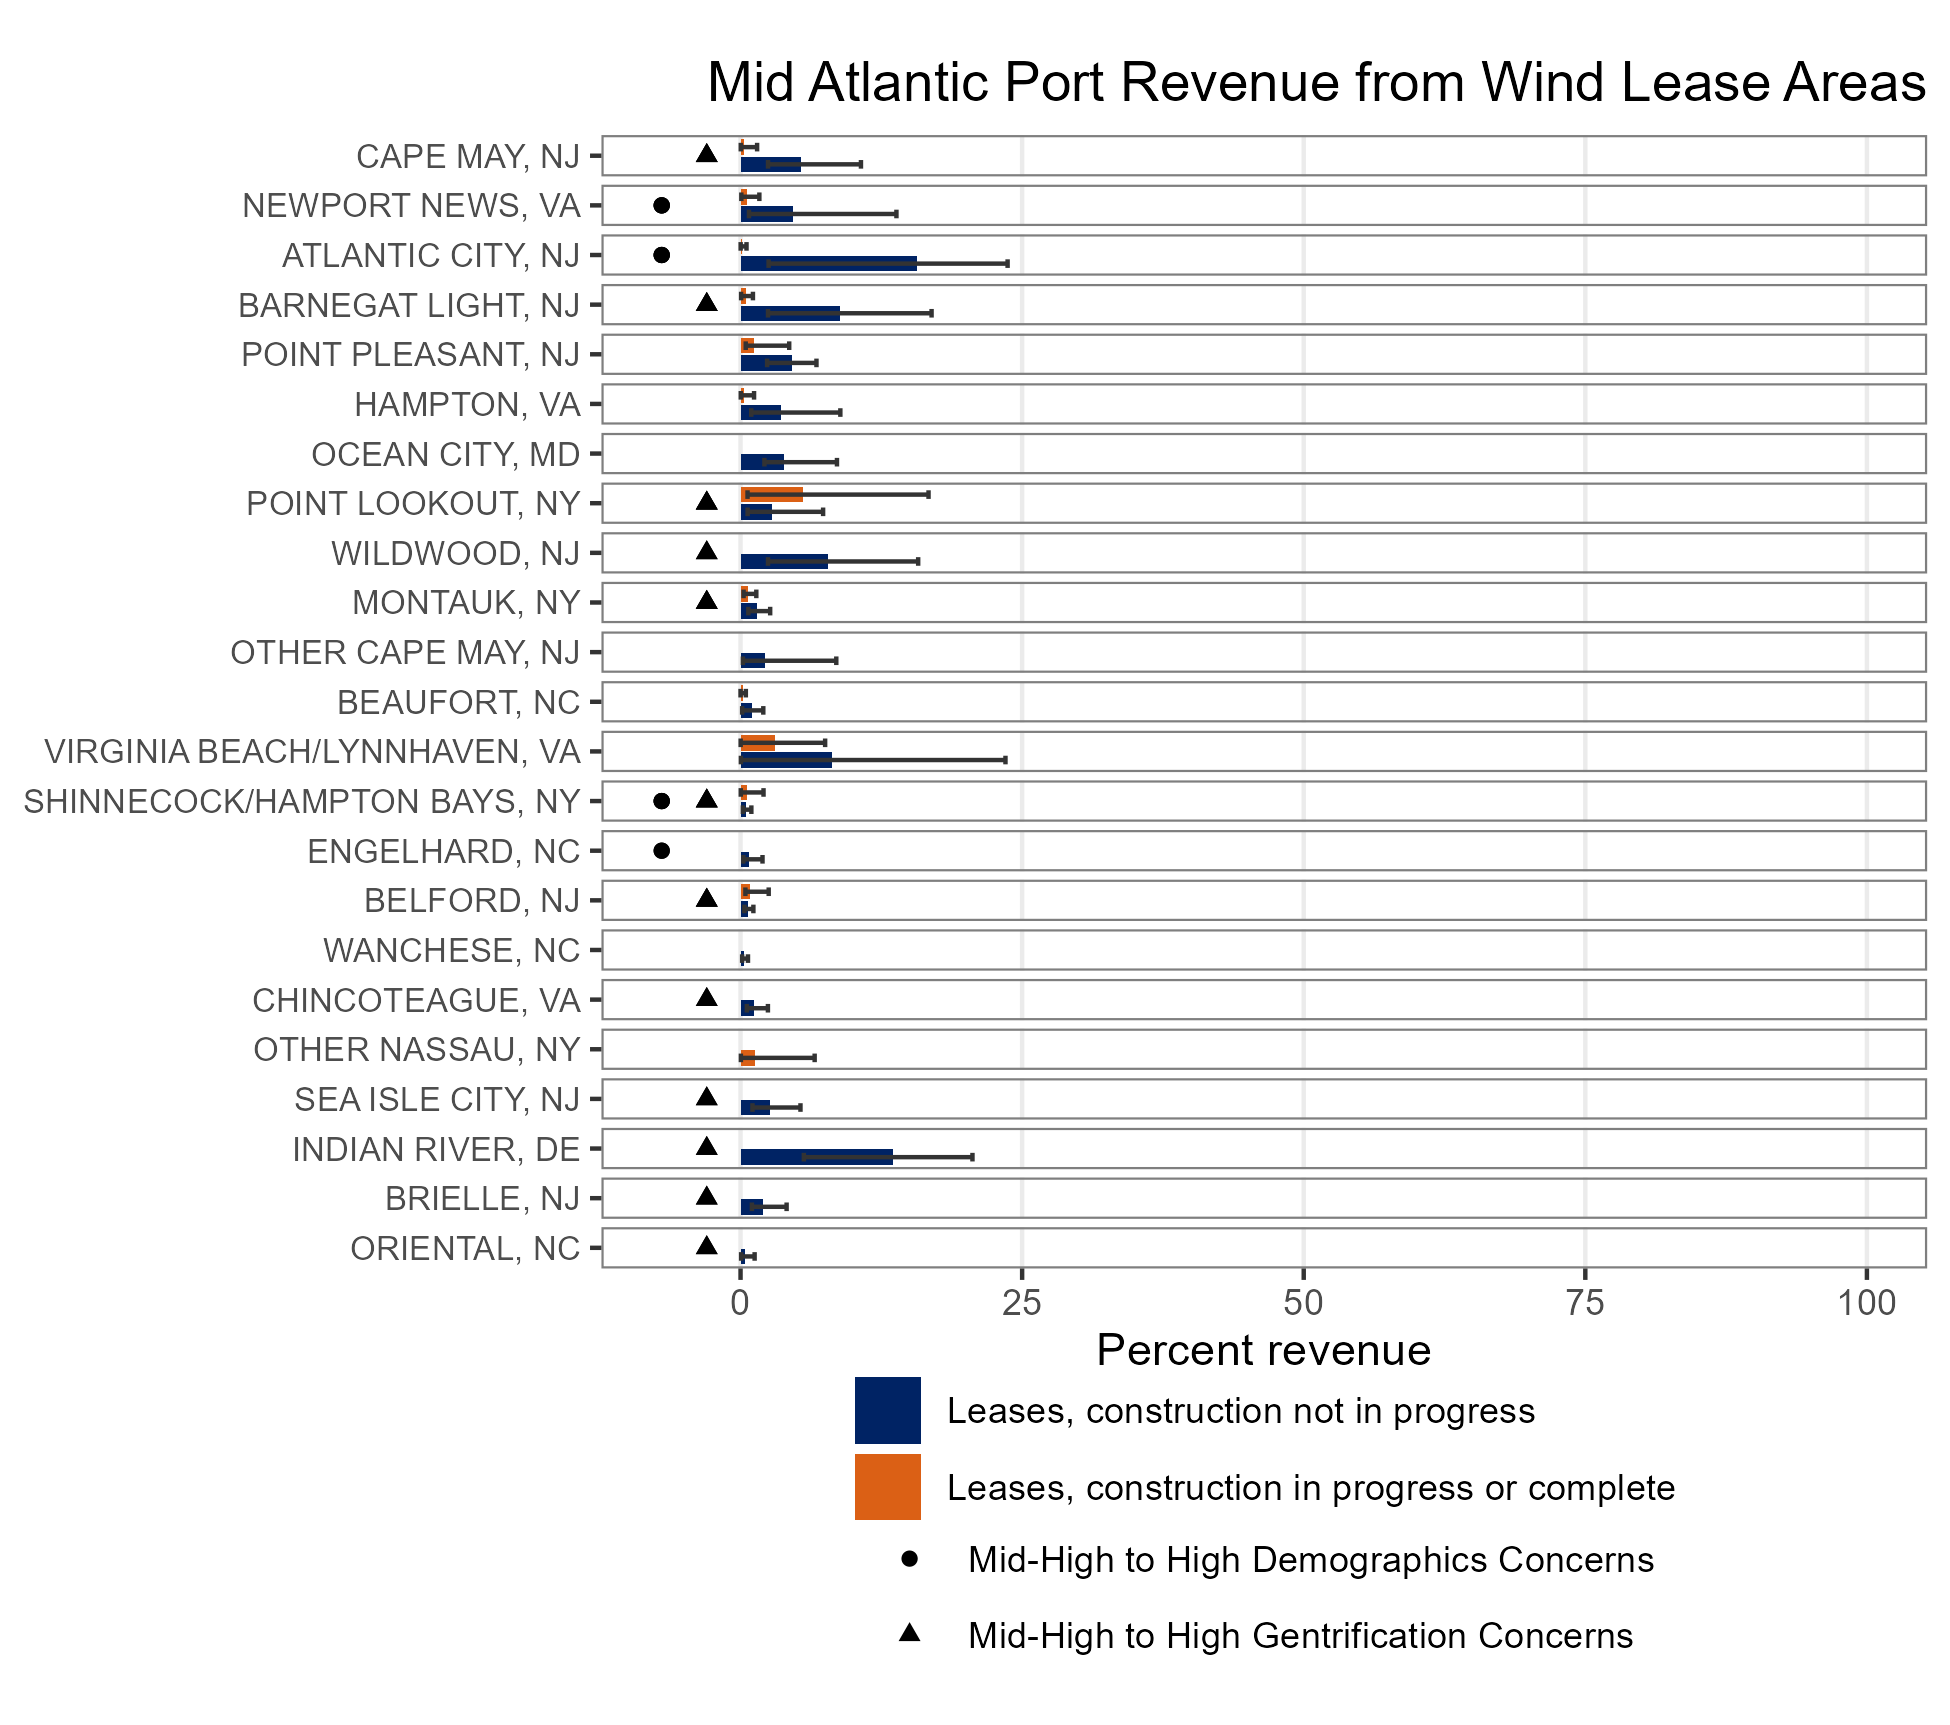
\includegraphics[width=1\linewidth,]{images/MidAtlantic/wea_port_rev_MidAtlantic_2026-03-26} \hfill{}

\caption{Percent of Mid-Atlantic port revenue from wind lease areas from leases not under construction (blue) and active leases (orange). Note that North Carolina fisheries management is split between the Northeast and Southeast, and this plot only includes data reported to the Northeast Fisheries Science Center.}\label{fig:wea-port-rev}
\end{figure}

Based on federal vessel logbook data, Point Lookout, NY (5.5\% average, 17\% maximum) and Virginia Beach, VA (3\% average, 7.5\% maximum) have the highest potential revenue loss from the Active Projects based on 2008-2024 total port fisheries revenue. Fewer Mid-Atlantic ports are affected by the Active Projects to date, as most are in the southern New England region, with the exception of CVOW and Empire Wind 1 (Fig. \ref{fig:wea-port-rev}). Additional fishing revenue may be affected as more areas historically used for fishing are developed for offshore wind energy.

In response to Council request, we also \href{https://noaa-edab.github.io/catalog/wind_port.html}{present information} on the New England ports that land MAFMC-managed species within the wind lease areas. This information can help fisheries managers better understand how MAFMC-managed species may be more broadly affected by offshore wind development. Seven New England ports attribute the majority of their landings within the wind lease areas to MAFMC-managed species (Fig. \ref{fig:wind-rev}); note that two of these ports do not have a majority of MAFMC-managed landings when only the Active Project areas are considered. Additionally, the Active Projects account for less than 8\% of total revenue in these seven ports. Future analyses should also consider that the impacts of offshore wind development may unevenly affect individual operators, with some permit holders deriving a much higher proportion of revenue from wind areas than the port-based mean.

\begin{figure}[T]

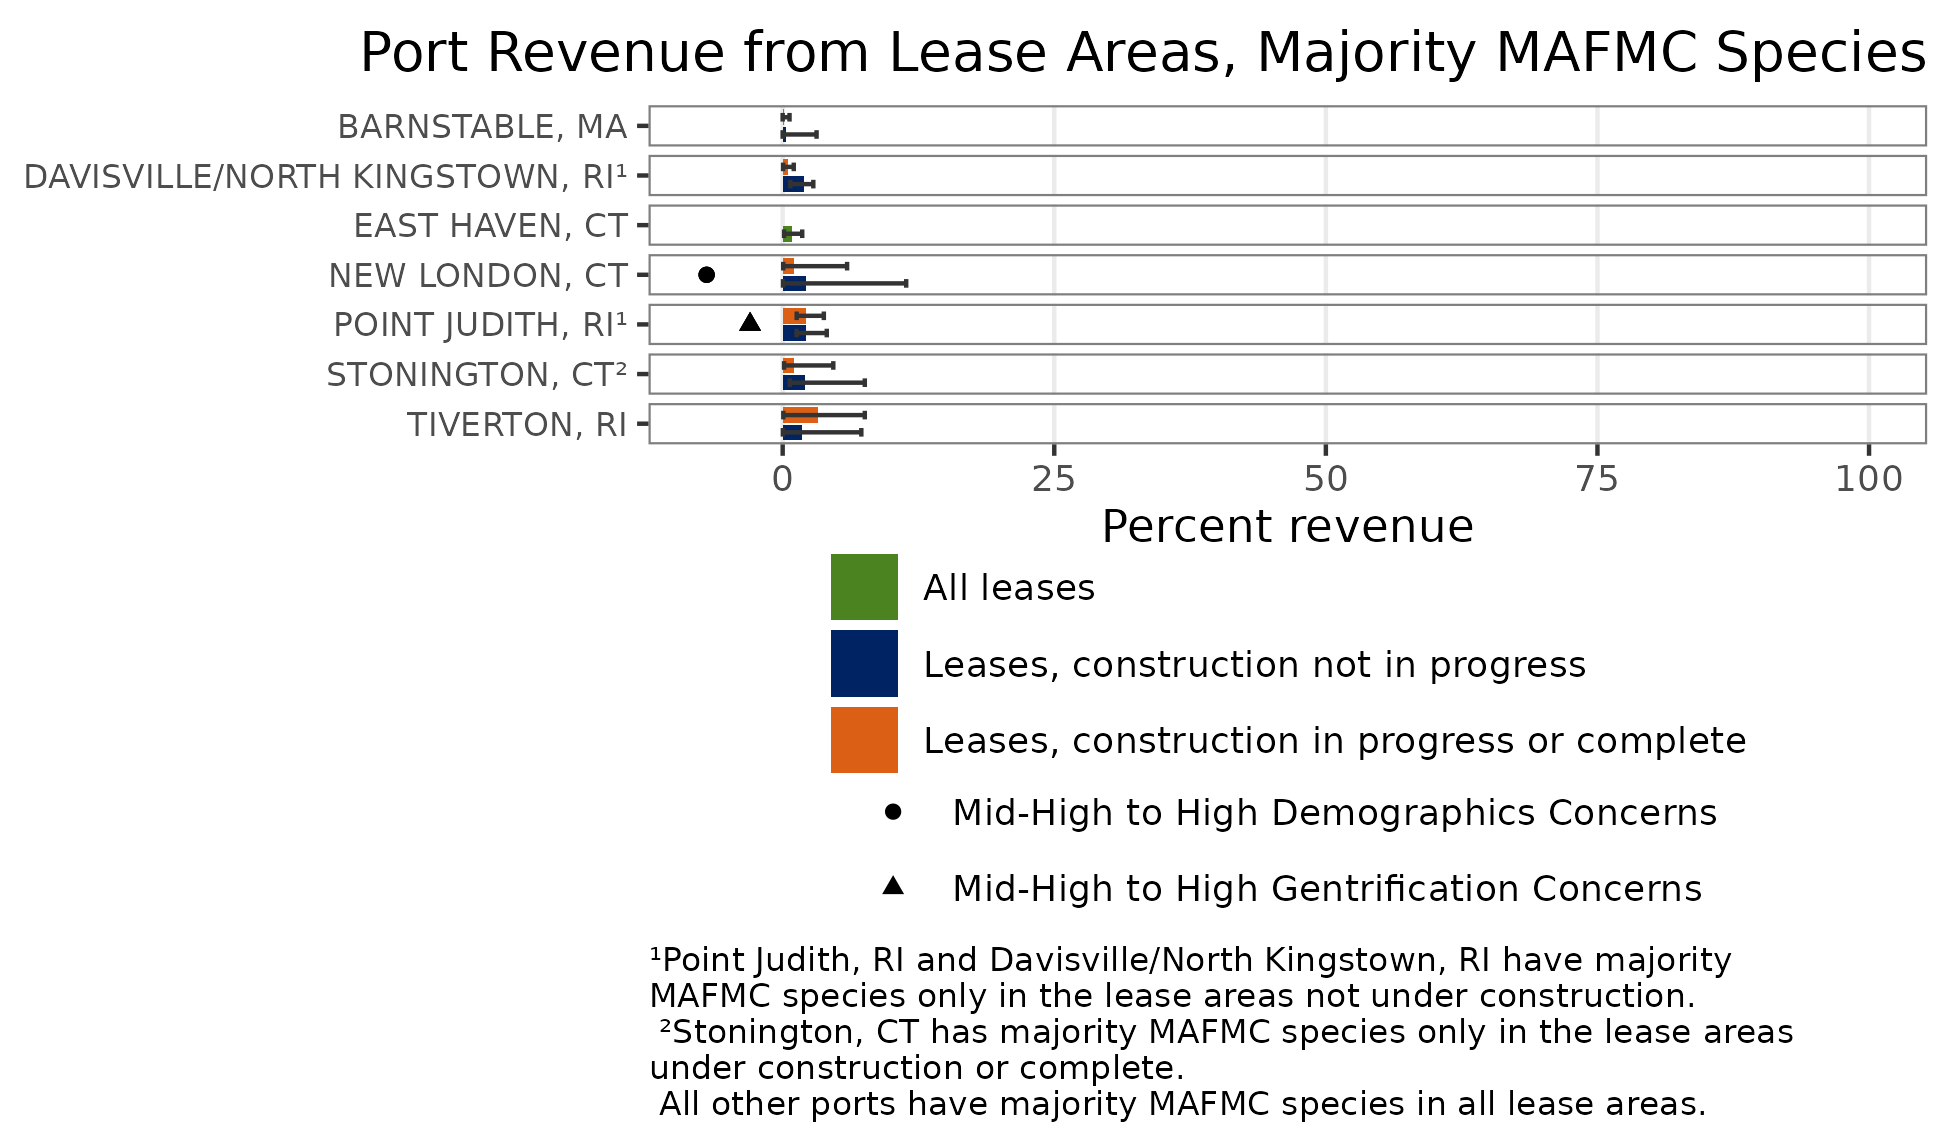
\includegraphics[width=1\linewidth,]{images/MidAtlantic/newengland_mafmc} \hfill{}

\caption{Percent of port revenue from wind lease areas for New England ports that land a majority of Mid-Atlantic Fishery Management Council-managed species within the wind lease areas. Percent of revenue is shown for leases not under construction (blue), active leases (orange), and all leases (green).}\label{fig:wind-rev}
\end{figure}

If all proposed projects are developed, BOEM reports that cumulative offshore wind development could have moderate impacts on low-income members of communities who work in the commercial fishing and for-hire fishing industry due to disruptions to fish populations, restrictions on navigation and increased vessel traffic, and exacerbation of existing vulnerabilities of low-income workers to economic impacts.

Top fishing communities with both landings from the Active Projects (i.e., Point Lookout, NY and Newport News, VA) and \href{https://noaa-edab.github.io/catalog/engagement.html}{socio-demographic or gentrification concerns} should be recognized as having additional vulnerability from Active Projects. To reduce further social and economic impacts and aid in the resilience and adaptive capacity of these communities, this vulnerability should be considered in decision making. Historically, the introduction of new industries can trigger industrial and socioeconomic gentrification of fishing ports. Competition for port space and potential pivoting of space use for offshore wind development should be monitored closely to ensure fishing communities are not adversely impacted. Additionally, offshore wind could increase recreational fishing opportunities at the turbines, potentially creating a demand for additional tourism, recreational fishing and boating port space in communities already balancing these uses with commercial fishing infrastructure (e.g., Virginia Beach, VA, Montauk, NY and Barnegat Light, NJ). Socio-demographic concerns also highlight communities where further resources are needed to reach underserved and underrepresented groups and create opportunities for, and directly involve, these groups in the decision-making process.

\subsubsection{Implications}\label{implications-6}

Current plans for buildout of offshore wind in a patchwork of areas spreads the impacts differentially throughout the region (Fig. \ref{fig:wind-dev-cumul}). Up to 6\% of maximum annual fisheries revenue for major Mid-Atlantic commercial species in lease areas could be forgone or reduced and associated effort displaced when the Active Projects are developed. Displaced fishing effort can alter fishing area, timing, and method patterns, which can in turn change habitat, species (managed and protected), and fleet interactions. Several factors, including fishery regulations, fishery availability, and user conflicts affect where, when, and how fishing effort may be displaced, along with impacts to and responses of affected fish species.

Proposed wind development areas interact with the region's federal scientific surveys. Scientific surveys are impacted by offshore wind in four ways:
1. Exclusion of NOAA Fisheries' sampling platforms from the wind development area due to operational and safety limitations.
2. Impacts on the random-stratified statistical design that is the basis for scientific assessments, advice, and analyses.
3. Alteration of benthic and pelagic habitats, and airspace in and around the wind energy development, requiring new designs and methods to sample new habitats.
4. Reduced sampling productivity through navigation impacts of wind energy infrastructure on aerial and vessel survey operations.

Increased vessel transit between stations may decrease data collections that are already limited by annual days-at-sea day allocations. In the Northeast region, 14 \href{https://noaa-edab.github.io/catalog/osw_survey_impact.html}{NEFSC surveys} overlap with offshore wind development projects at varying capacities, with each of the 38 existing lease areas overlapping between 4-14 surveys. The Active Projects overlap between 10-12 surveys. Implementation of the region-wide survey mitigation program is underway with requirements to mitigate impacts to surveys included as a condition of most project approvals.

Planned development \href{https://noaa-edab.github.io/catalog/persistent_hotspots.html}{overlaps NARW} mother and calf migration corridors and a significant foraging habitat that is used throughout the year (Fig. \ref{fig:whales-wind}). Turbine presence and extraction of energy from the system could alter local oceanography and may affect right whale prey availability. For example, persistent foraging hotspots of right whales and seabirds overlap on Nantucket Shoals, where unique hydrography aggregates enhanced prey densities. Two wind projects, SouthCoast Wind and Vineyard Northeast, currently intersect these hotspots on the southwestern corner of Nantucket Shoals and a prominent tidal front associated with invertebrate prey swarms important to seabirds and possibly right whales. However, neither of these projects have begun construction as of January 2026. Proposed wind development areas also bring increased vessel strike risk from construction and operation vessels. In addition, there are a number of potential impacts to whales from pile driving and operational noise such as displacement, increased levels of communication masking, and elevated stress hormones.

\begin{figure}[T]

{\centering 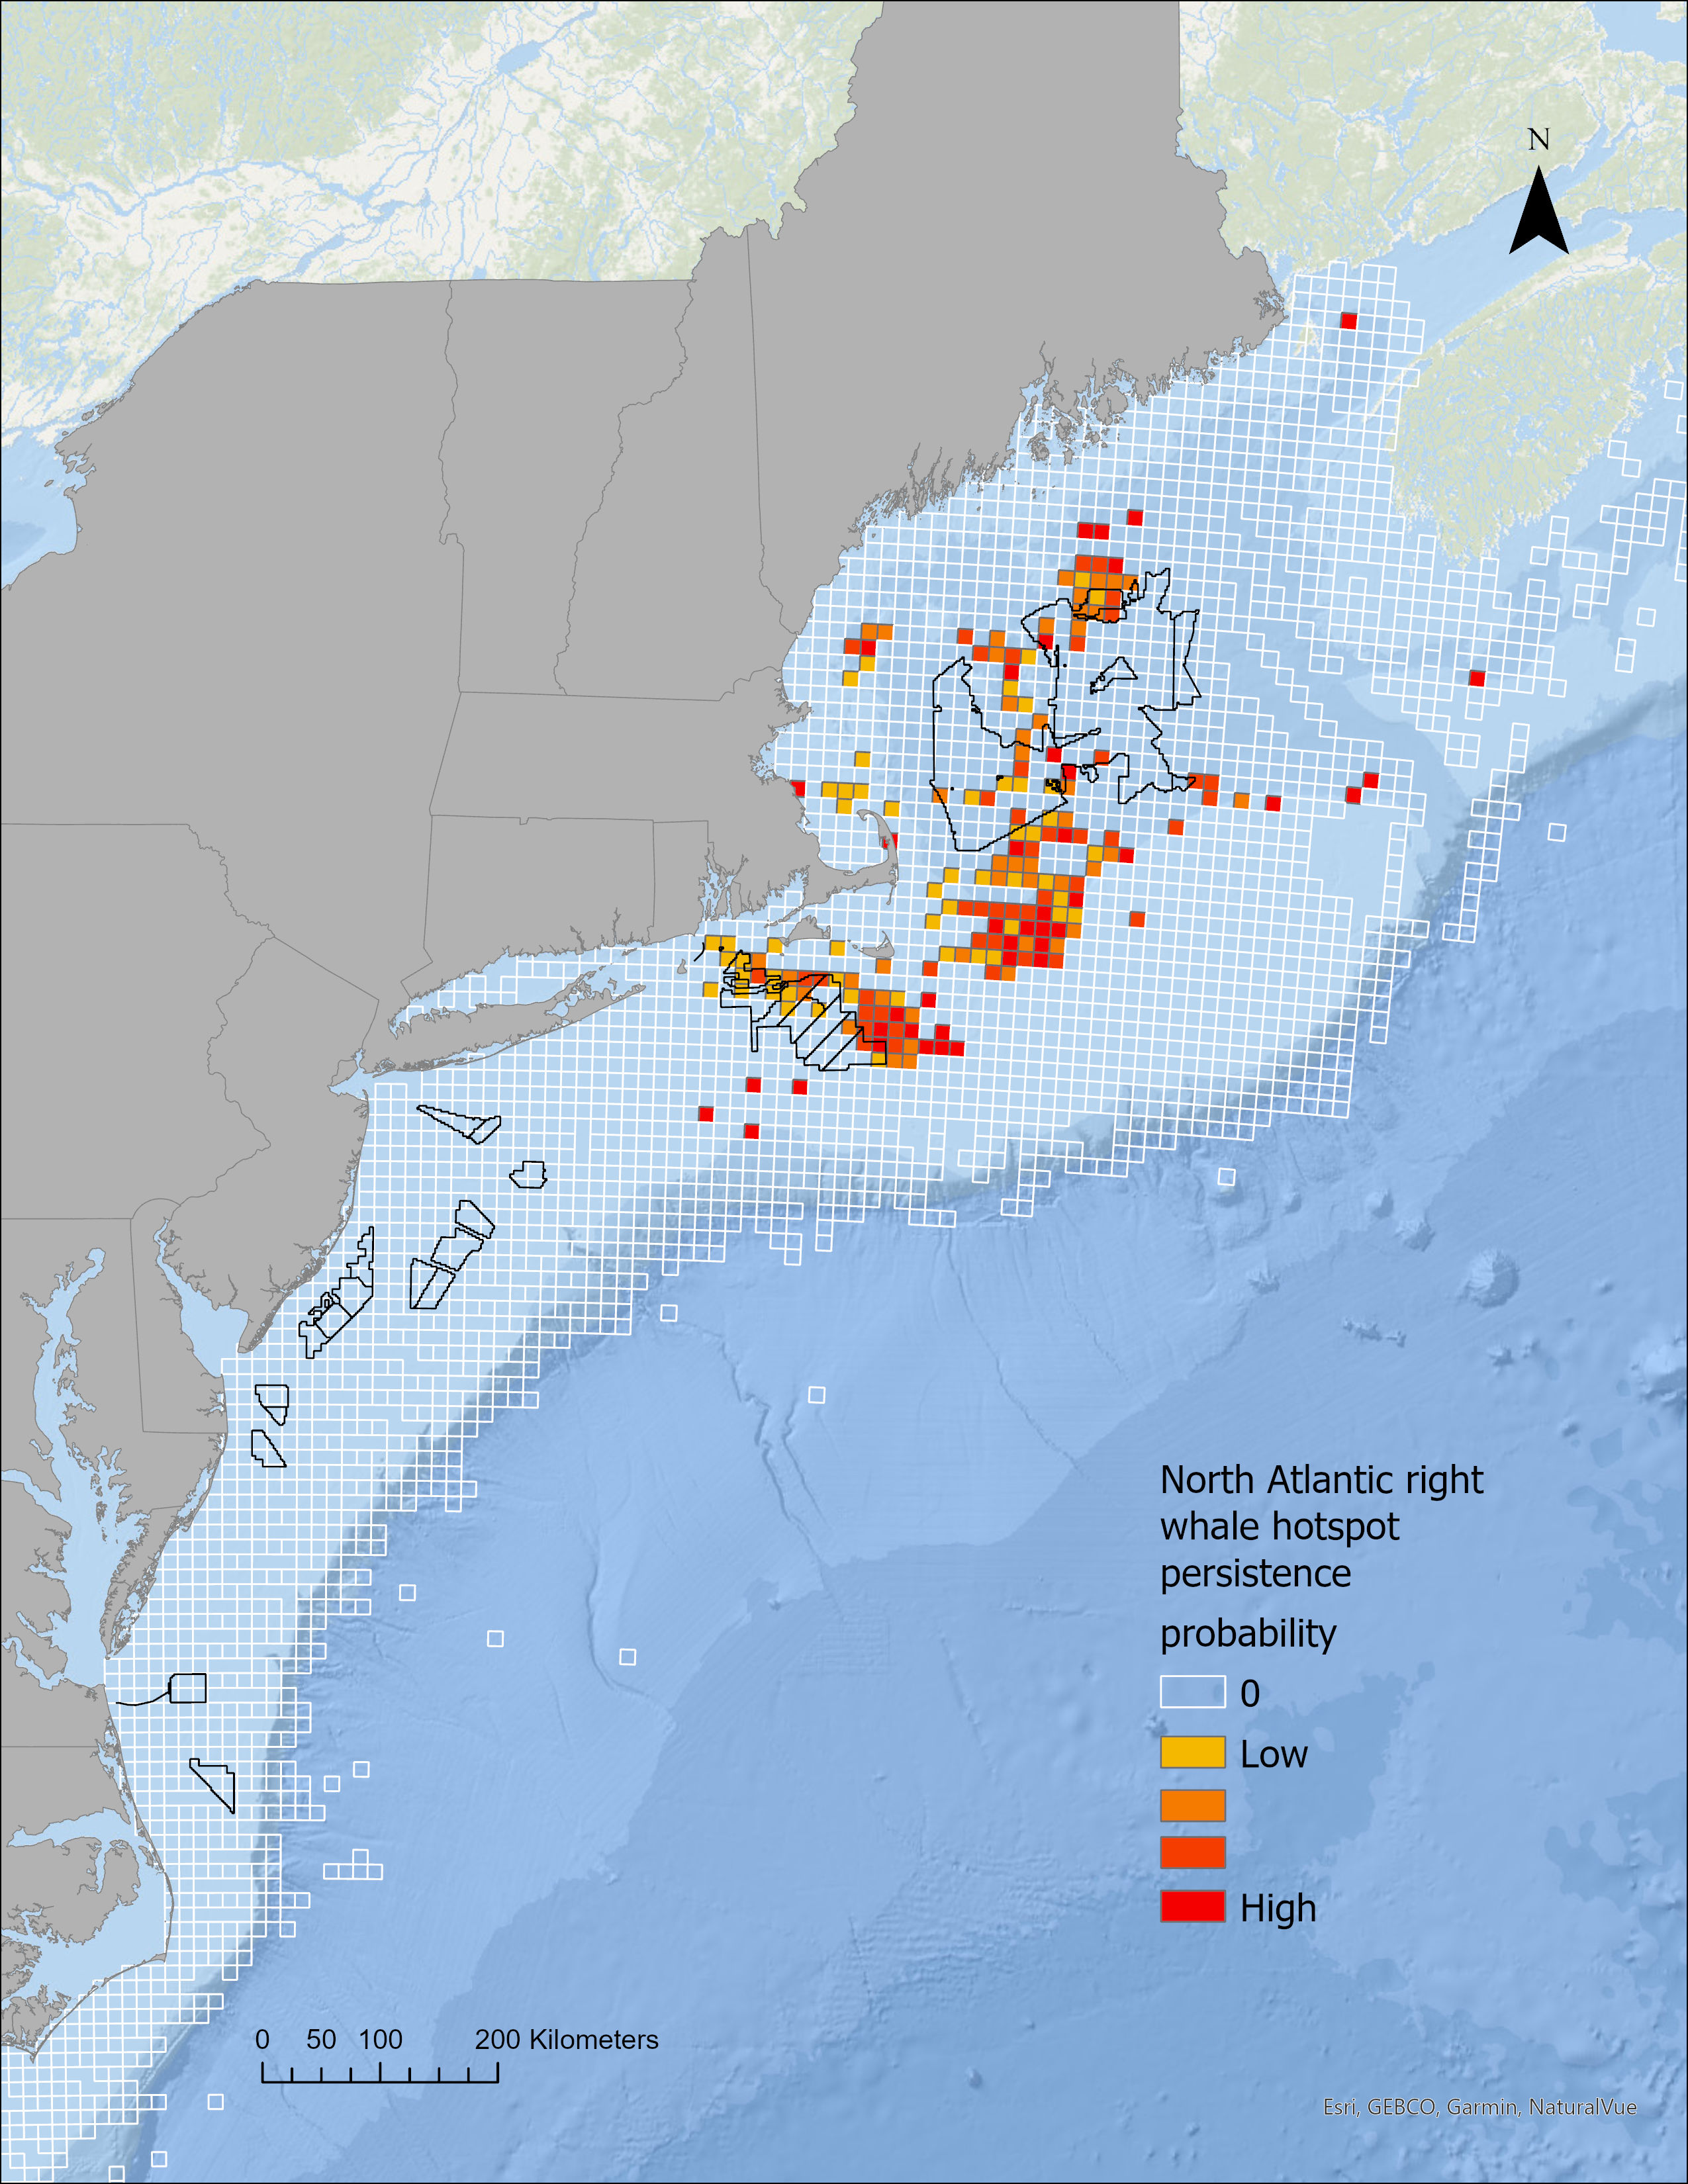
\includegraphics[width=0.55\linewidth,]{images/BothReports/NARW_hotspots_final_2024} 

}

\caption{North Atlantic Right Whale persistent hotspots (red shading) and wind lease areas (black outlines).}\label{fig:whales-wind}
\end{figure}

The increase of offshore wind development can have both positive (e.g., employment opportunities) and negative (e.g., space-use conflicts) effects. Continued increase in coastal development and gentrification pressure has resulted in loss of fishing infrastructure space within ports. Understanding these existing pressures can allow for avoiding and mitigating negative impacts to our shore support industry and communities dependent on fishing. Some of the communities with the highest fisheries revenue overlap with offshore wind development areas that are also vulnerable to gentrification pressure are Beaufort, NC, and Cape May, Barnegat Light, and Long Beach, NJ.

\paragraph{Marine Aquaculture}\label{marine-aquaculture}

Aquaculture fisheries and federally-managed fisheries could compete with or benefit each other with spatial access, shoreside infrastructure, or the supply of seafood. Unlike offshore wind, offshore aquaculture is not regulated by any federal leasing program but is permitted via the U.S. Army Corps of Engineers and the U.S. EPA. Currently, there are no federally-permitted aquaculture projects in the Northeast U.S. The marine aquaculture industry of the Northeast currently occurs in nearshore waters which are regulated by state leasing and permitting processes and federal permitting processes, as applicable. Analyses are needed to quantify the nearshore spatial distribution of aquaculture in the Northeast.

\subsubsection{2025 Highlights}\label{highlights}

This section intends to provide a record of \href{https://noaa-edab.github.io/catalog/observation_synthesis_2025.html}{noteworthy observations reported in 2025} across the Northeast U.S. region. The full ecosystem and fisheries impacts of many of these observations are still to be determined. They should, however, be noted and considered in future analyses and management decisions.

The Northeast U.S. region experienced colder than average ocean temperatures, despite record warm \href{https://www.ncei.noaa.gov/news/global-climate-202513}{global} ocean and air temperatures. Similar to 2024, oceanographic and ecological conditions reflected cooler water and changing species abundance, distribution, and timing.

\paragraph{Northwest Atlantic Phenomena}\label{northwest-atlantic-phenomena}

The below average temperatures observed in 2024 persisted into 2025, although there are seasonal and local exceptions to this pattern (Fig. \ref{fig:slopesea}), however, the waters were not as fresh as recorded in 2024. Winter bottom temperatures were also below average across much of the Northeast Shelf (Fig. \ref{fig:slopesea}). Multiple oceanographic and atmospheric factors can contribute to these cooler conditions including a more southerly Gulf Stream and higher proportions of Labrador Slope and Scotian Shelf water entering the system.

\begin{figure}[T]

{\centering 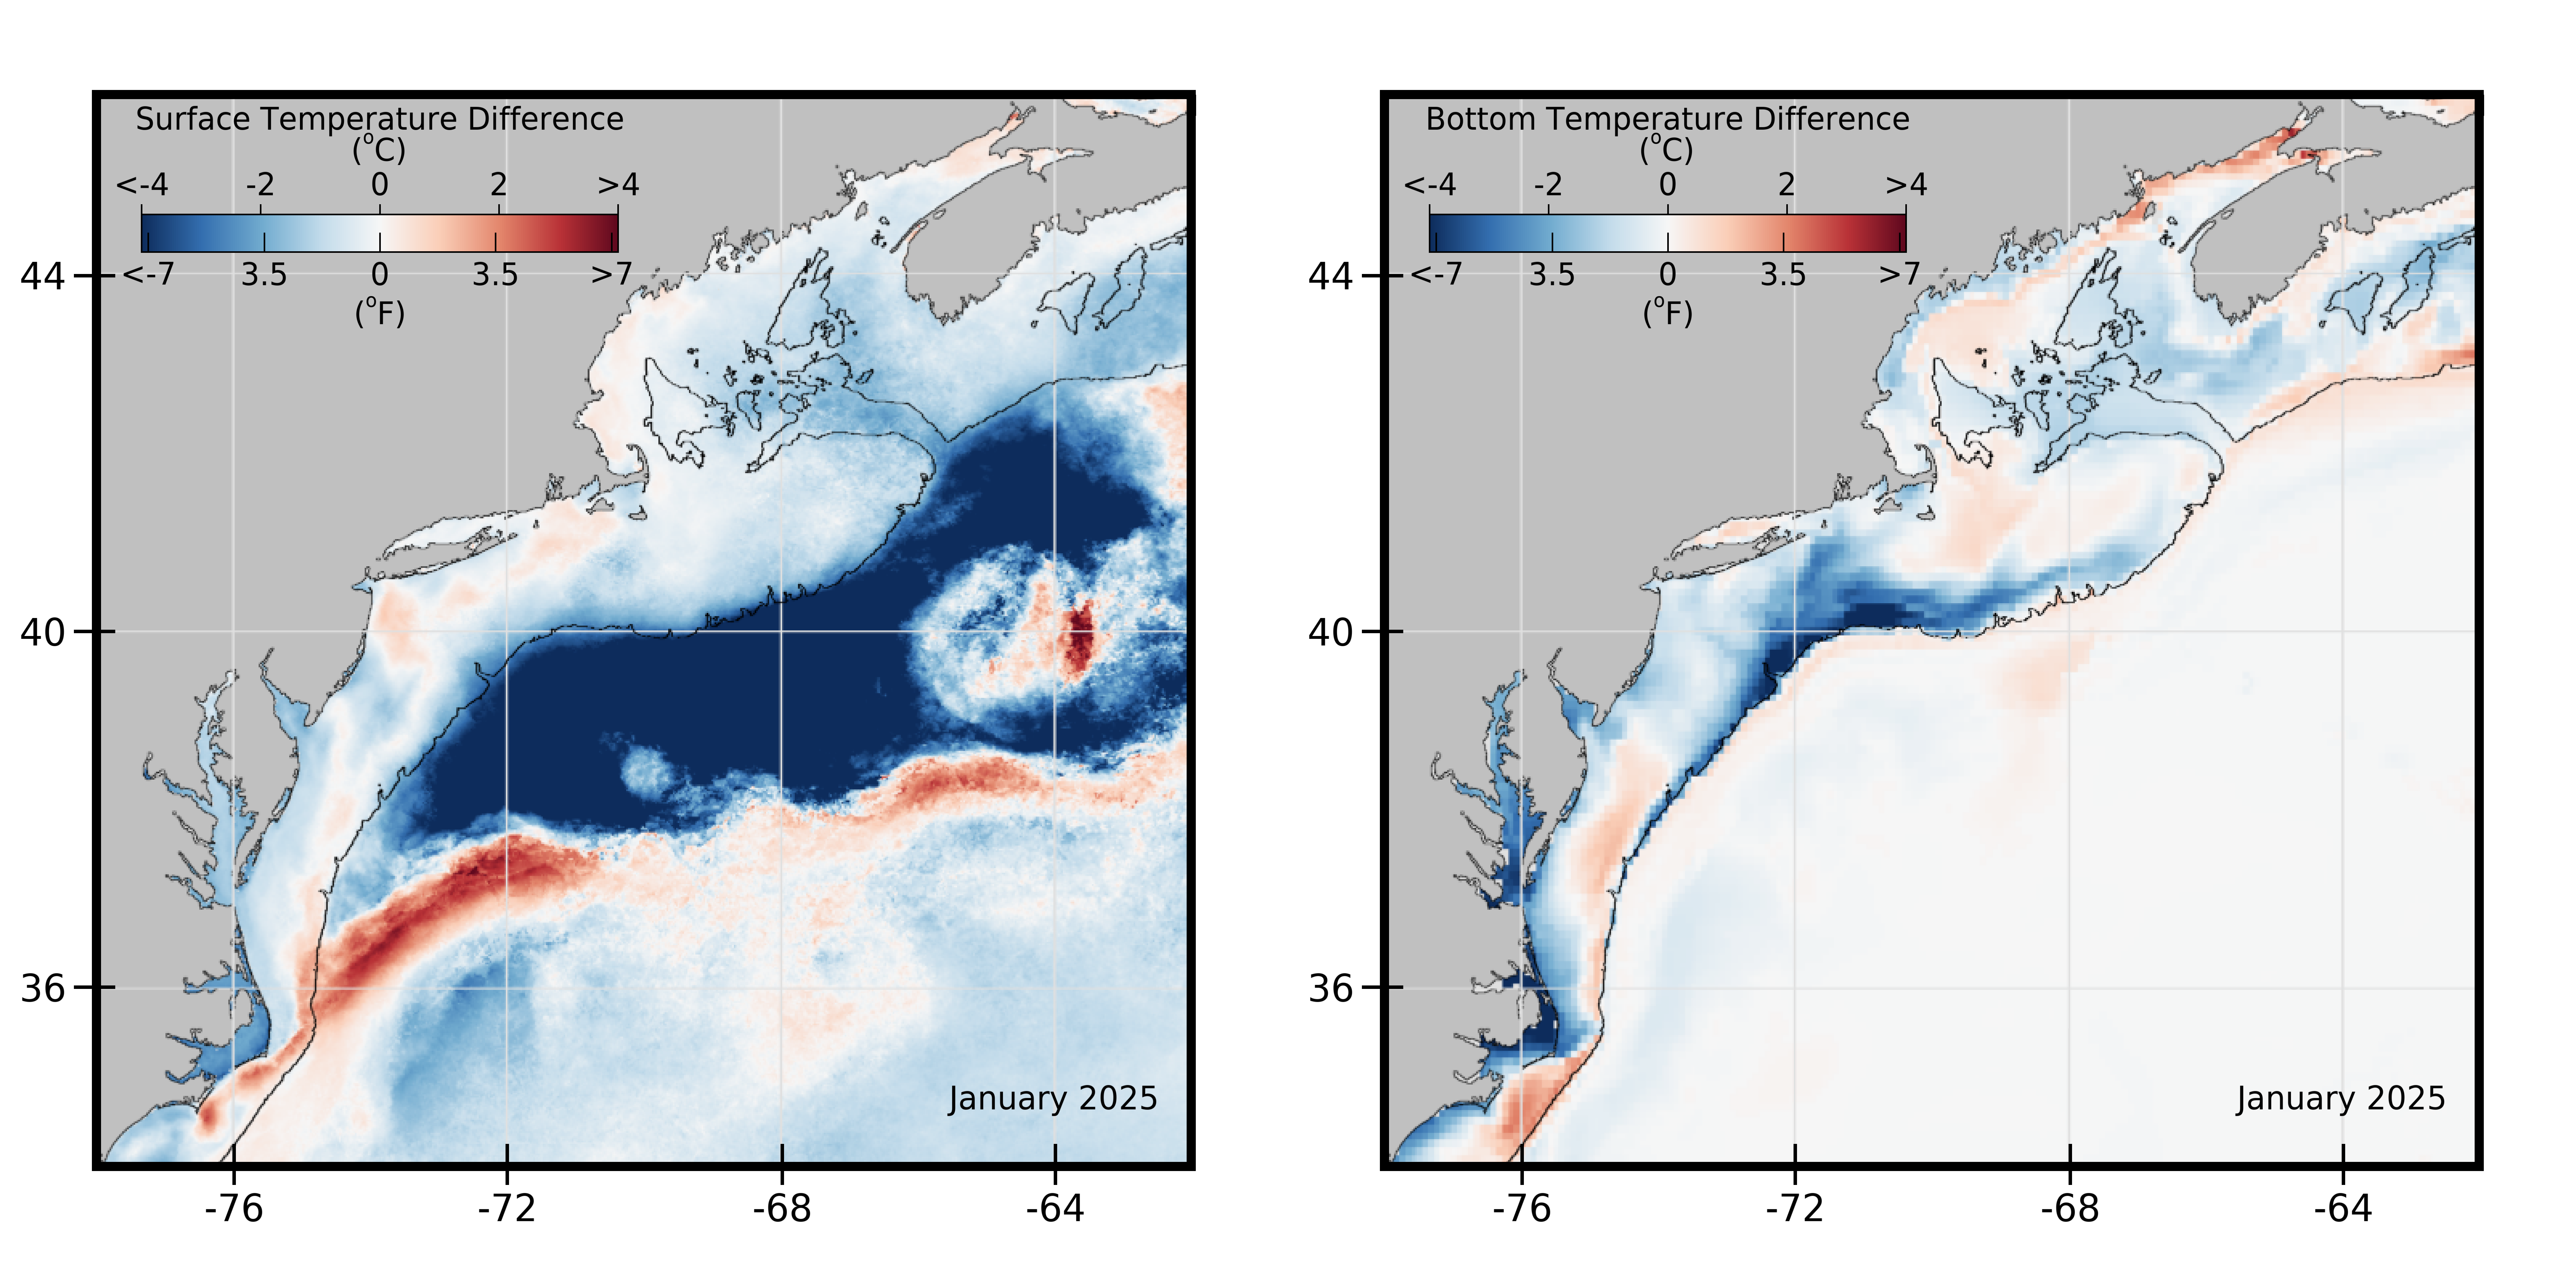
\includegraphics[width=1\linewidth,]{images/BothReports/processed_Highlights_2026-SST_Anomaly-202501-NES} 

}

\caption{January 2025 sea surface (left) and bottom (right) temperature differences compared to the January climatological means. Sea Surface Temperature (SST) is from the NOAA Advanced Clear-Sky Processor for Ocean (ACSPO) Super-collated SST (climatology range 2000-2020); Bottom temperature is from the GLORYS reanalysis model (climatological range 1990-2020).}\label{fig:slopesea}
\end{figure}

In 2024, the Gulf of Maine \href{https://noaa-edab.github.io/catalog/slopewater.html}{source water} entering through the Northeast Channel was near equal proportions of Warm Slope Water and cooler Labrador Slope Water (Fig. \ref{fig:slopewater}); data are still being processed for 2025. The colder conditions \href{https://noaa-edab.github.io/catalog/observation_synthesis_2024.html}{observed in 2024} continued into 2025 and contributed to the increased size and colder temperatures of the Mid-Atlantic \href{https://noaa-edab.github.io/catalog/cold_pool.html}{Cold Pool}.

\begin{figure}[T]

{\centering 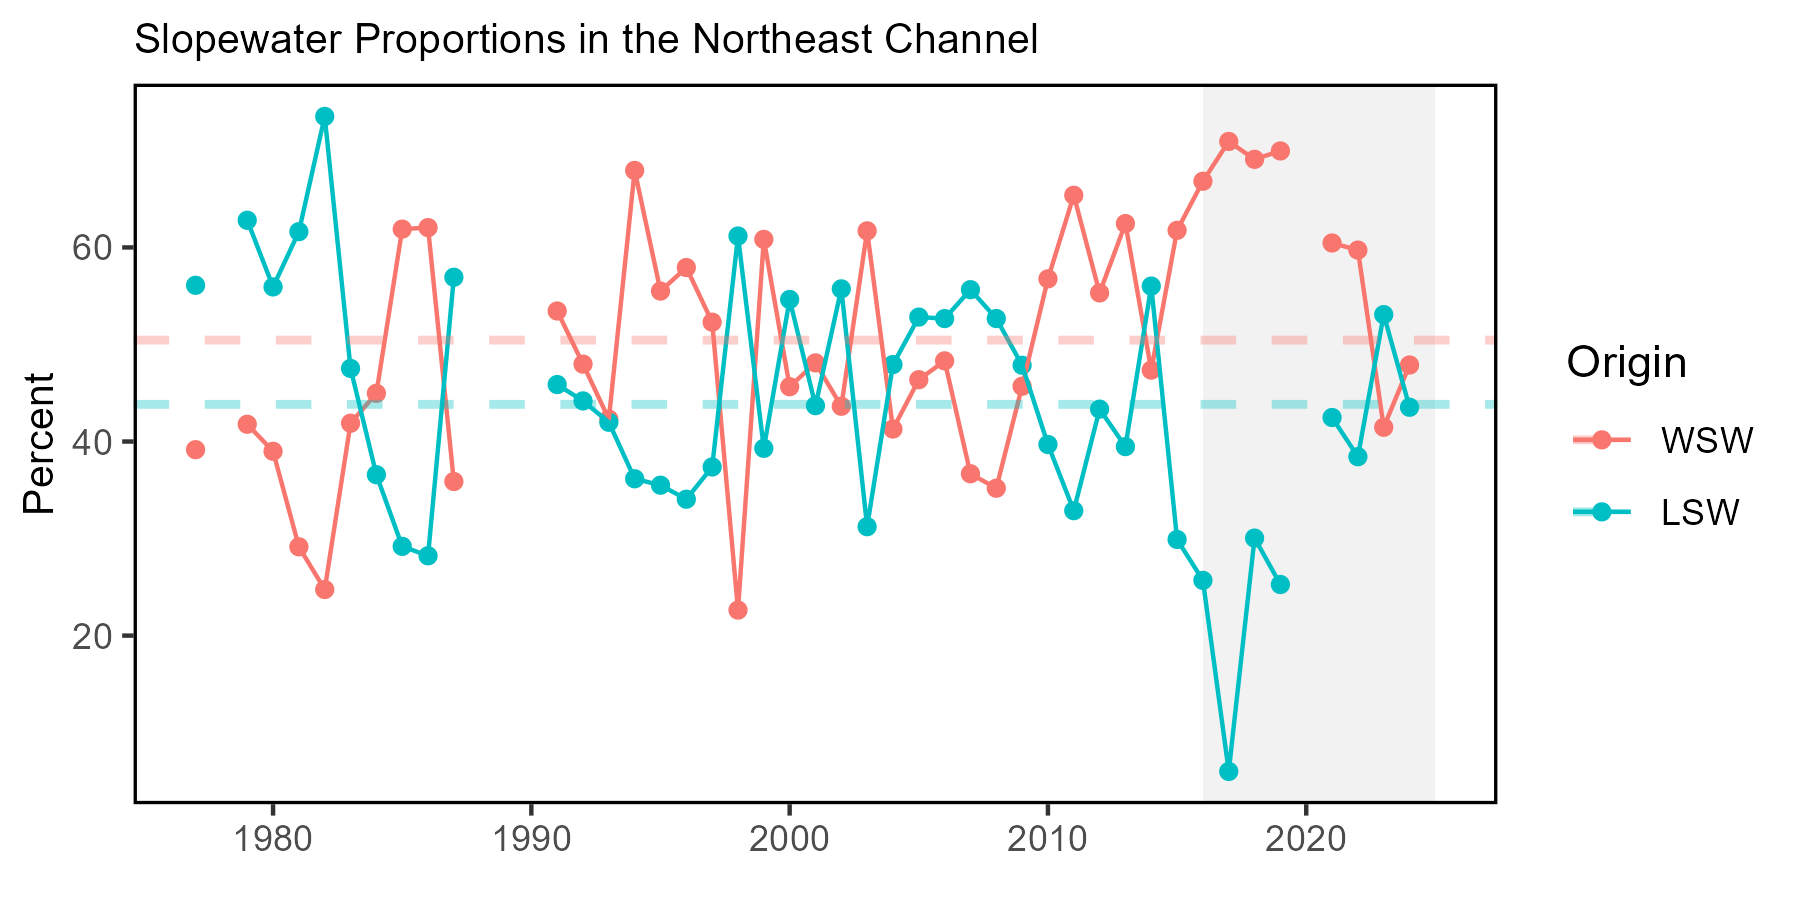
\includegraphics[width=1\linewidth,]{images/BothReports/slopewater_BothReports_2026-03-26} 

}

\caption{The proportion of Warm Slope Water (WSW) and Labrador Slope Water (LSW) entering the Gulf of Maine through the Northeast Channel from 1977 to 2024. The red and teal dashed lines represent the long-term proportion averages for the WSW and LSW respectively.}\label{fig:slopewater}
\end{figure}

2025 total primary production was below average in Georges Bank and the Mid-Atlantic due to lower phytoplankton biomass and cooler sea surface temperatures. \href{https://noaa-edab.github.io/catalog/chl_pp.html?q=phyt\#chl_pp}{Phytoplankton biomass} (shown as chlorophyll a concentration) was also below average for much of 2025 (Fig. \ref{fig:chl-anom}). In particular, the winter-spring bloom period, which typically accounts for a significant proportion of total annual phytoplankton production, was shorter in duration and lower in magnitude across the entire Northeast shelf region. The fall bloom period was above average in the Gulf of Maine and Georges Bank, but near average in the Mid-Atlantic.

\begin{figure}[T]

{\centering 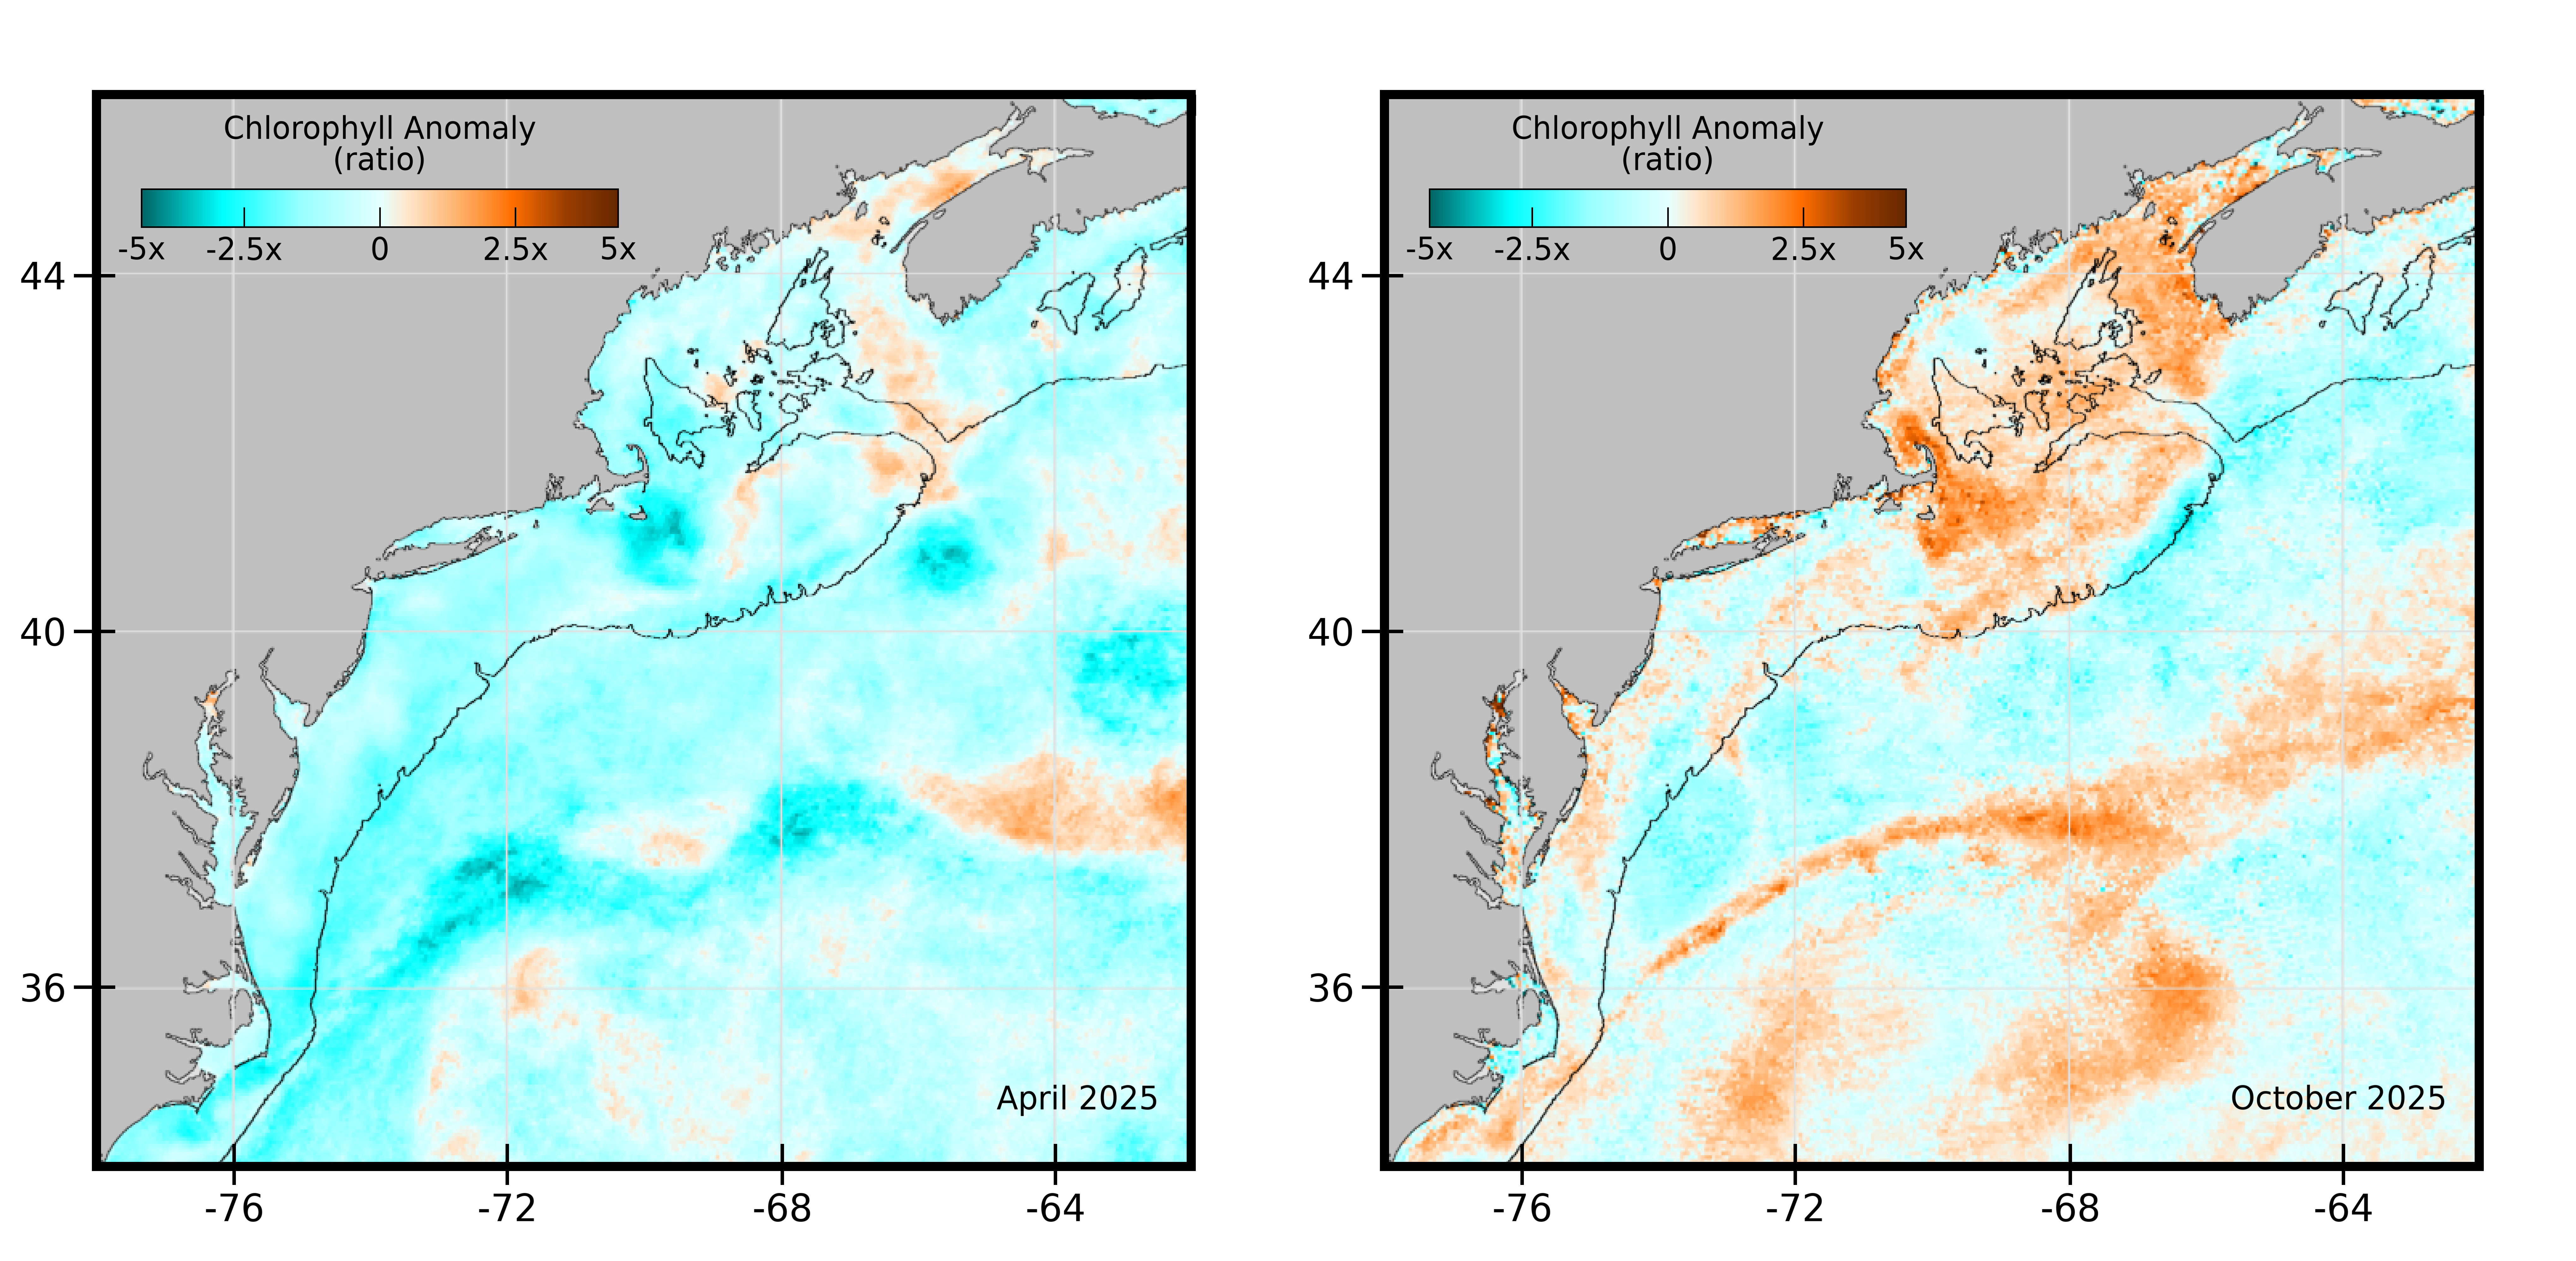
\includegraphics[width=1\linewidth,]{images/BothReports/processed_Highlights_2026-CHL_Anomaly-202504-NES} 

}

\caption{Chlorophyll anomalies shown as the ratio of the monthly concentration compared to the climatological mean (1998-2020) for April (left) and October (right), 2025.}\label{fig:chl-anom}
\end{figure}

Hurricane Erin was the most notable storm in the region in 2025 and caused significant shoreside and oceanographic disturbances despite not making landfall in the Northeast. Its strong winds and large size caused mixing and weakened stratification throughout the Mid-Atlantic resulting in cooler than average surface waters across the shelf and into the Slope Sea. Along the coast, beaches from Maryland to Maine were closed due to rough surf, large waves, and rip currents, while coastal flooding led to road closures and several water rescues, particularly in New Jersey. Beach erosion was significant in some locations.

\paragraph{Northeast Shelf and Local Phenomena}\label{northeast-shelf-and-local-phenomena}

The shift to cooler waters in 2024-2025 is likely linked to multiple observations across the Northeast Shelf including the uncommon presence of Arctic zooplankton species in the Gulf of Maine, delayed migration of many species, and redistribution of some species. These shifts could affect the availability of some species to surveys or fishing, although aggregate species distributions in the cooler 2024-2025 period continue to trend towards more northern and deeper waters (Fig. \ref{fig:species-dist}).

Mid-Atlantic scallops in the Elephant Trunk region are showing positive signs following the \href{https://noaa-edab.github.io/catalog/observation_synthesis_2023.html}{documented die-off}. Two-year olds observed in 2024 had good survival into the 2025 survey. The Elephant Trunk region is scheduled to reopen in 2026. There was also good survival of the \href{https://noaa-edab.github.io/catalog/observation_synthesis_2024.html}{2024 recruits} in the southeastern \href{https://noaa-edab.github.io/catalog/observation_synthesis_2025.html}{Nantucket Lightship Area in 2025}. In contrast, large numbers of the scallop predator \emph{Asterias vulgaris} sea stars were linked to an increased sea scallop mortality in 2024 and 2025 on Georges Bank.

Several members of the fishing community noted changes in species composition, distribution, and timing in their typical fishing grounds and attributed it to the cooler temperatures. These observations may not fully represent the entire ecosystem, but provide local context to recent events that may not be represented in other indicators. Some notable examples include:

\begin{itemize}
\tightlist
\item
  Several members of the fishing industry reported that it was a ``very good year'' for billfish. According to the Large Pelagic Survey, it was a record year for white marlin with more than 23,000 fish caught and released. Billfish effort may have been higher than usual due to the closure of the recreational bluefin tuna fishery in August 2025.
\item
  Chesapeake Bay anglers reported good catch of red drum in 2024, followed by low catch and even cold stunned red drum and spotted sea trout in 2025. Scientists working with charter captains in Chesapeake Bay reported low catch rates of striped bass and red drum from June-September, but higher catch rates in the early spring and fall.
\item
  Fishers attributed the delayed migration of black sea bass inshore, and scup migrating south for the winter using similar routes as in the early 1970s due to the cooler temperatures.
\item
  Members of the bluefish fishery in Rhode Island reported very low landings in 2025 attributed to changes in seasonal migration path or timing.
\item
  Some species, such as Atlantic mackerel, Illex squid and sandlance, were observed in higher abundance and wider distributions compared to recent years.
\item
  Fishers in the Gulf of Maine and Georges Bank had mixed reports of lobsters and good catch of sea scallops.
\item
  Fishers reported fewer warm water species in 2025 along the New Jersey coast. Others, however, noted more new species (e.g., pomapano, spadefish, triggerfish, Spanish and king mackerel) in Delaware Bay.
\item
  Anglers also observed low spring and summer catches of gamefish in Mid-Atlantic bays and on the shelf, and high concentrations of shark species near the coast.
\end{itemize}

In Chesapeake Bay, colder than average winter 2025 temperatures (Fig. \ref{fig:chesapeake-jan}) were reported by state agencies as a likely cause of higher blue crab mortality rates compared to the previous winter. Colder winters generally indicate good conditions for striped bass spawning, and while the striped bass juvenile index slightly increased, it was still well below the long-term average. Several years of low striped bass recruitment is a growing concern of fisheries managers. Factors that could be influencing striped bass recruitment include below average winter-to-spring freshwater flow and above average water temperatures combined with stressfully low dissolved oxygen values during the summer. The continued presence of invasive blue catfish and the effect they are having on blue crab, alosines, menhaden, and striped bass populations is also a management concern.

\begin{figure}[T]

{\centering 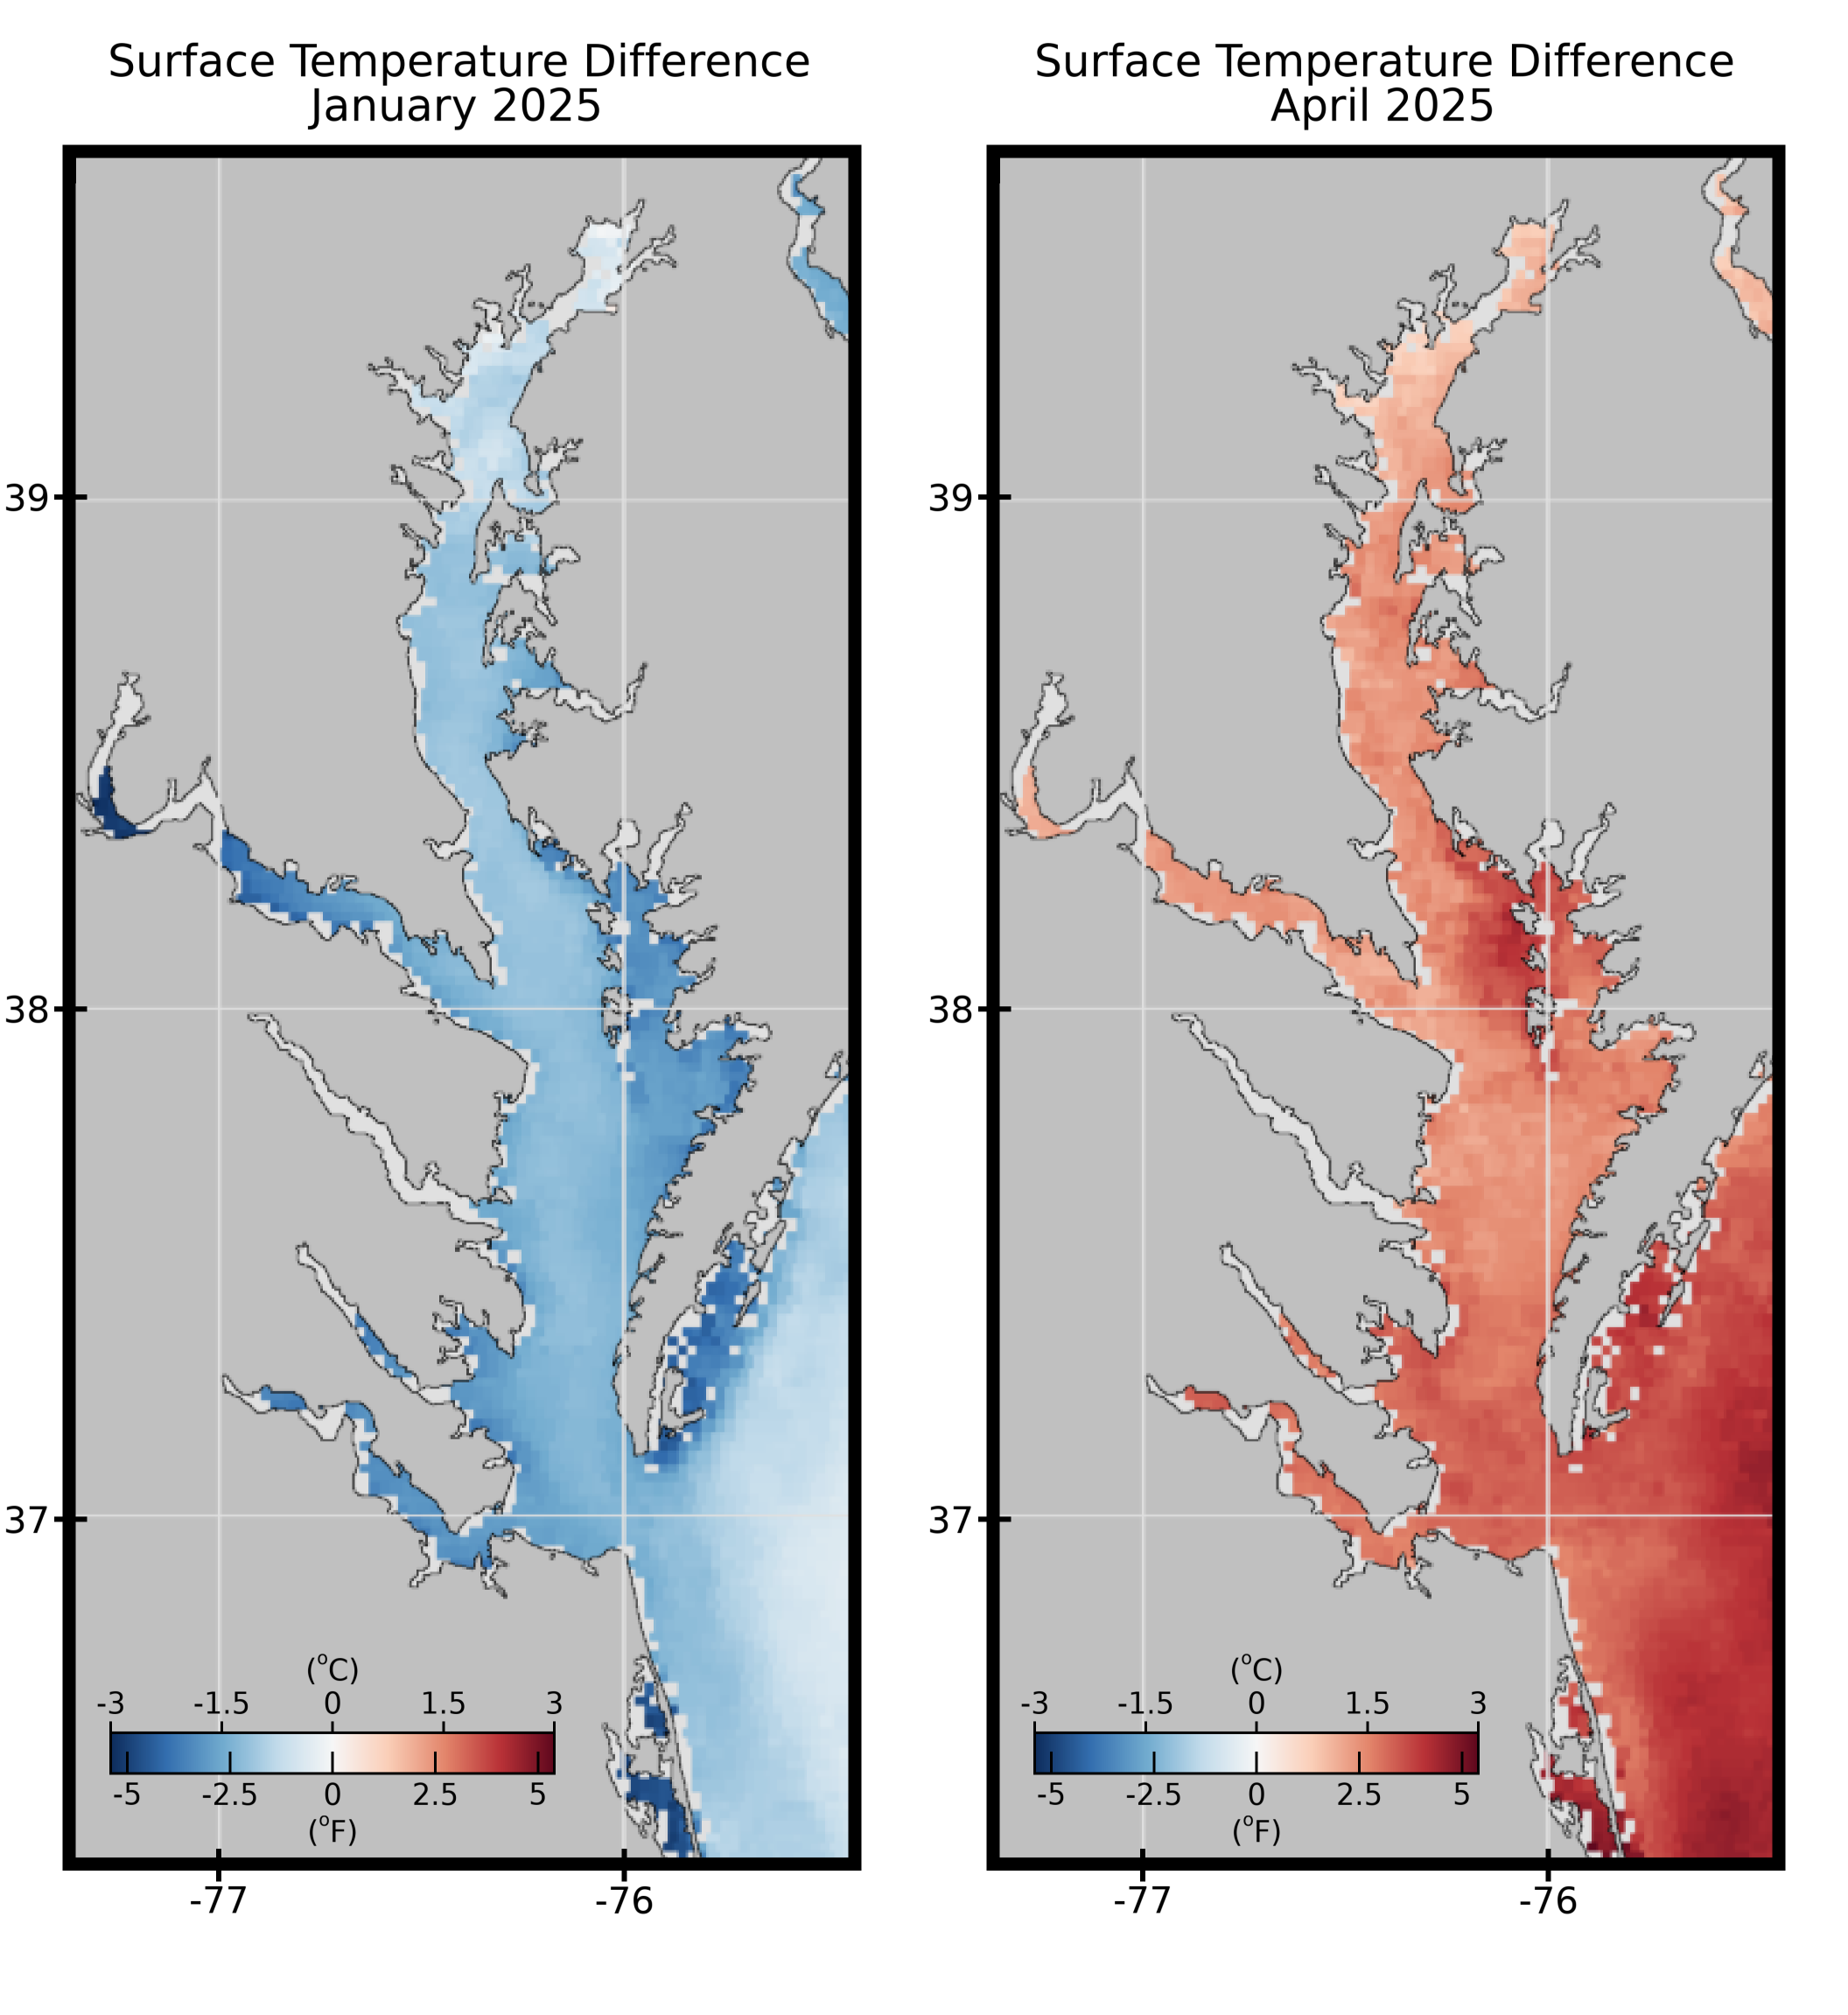
\includegraphics[width=0.5\linewidth,]{images/BothReports/processed_Highlights_2026-SST_Anomaly-202501-Ches_Bay.png} 

}

\caption{January 2025 (left) and April 2025 (right) sea surface temperature differences compared to the respective monthly climatological means. Sea Surface Temperature (SST) is from the NOAA Advanced Clear-Sky Processor for Ocean (ACSPO) Super-collated SST (climatology range 2000-2020).}\label{fig:chesapeake-jan}
\end{figure}

\href{https://noaa-edab.github.io/catalog/ocean_acidification.html}{Ocean acidification (OA)} risk in 2025 in the Mid-Atlantic was relatively low (Fig. \ref{fig:mab-oa}). There were few locations in 2025 where OA risk was high for Atlantic sea scallops, longfin squid, and pteropods. This is in contrast to the more prevalent OA risk events for these species in 2023 and 2024. \href{https://noaa-edab.github.io/catalog/gom_acidification.html}{Gulf of Maine surface OA risk} in 2025 was below 2024 levels, as indicated by aragonite saturation state (Ωa) at or near the climatological average (2006-2024).

\paragraph{Offshore Wind}\label{offshore-wind}

Offshore wind projects continue to be developed throughout the region. Information here represents the status as of the end of January 2026. In Southern New England, South Fork Wind Farm remains the first and only commercial scale project under operation (12 turbines), Vineyard Wind 1 and Revolution Wind continued construction, and Sunrise Wind began offshore construction (Fig. \ref{fig:wind-dev-cumul}). In the New York Bight, Empire Wind 1 began offshore construction (Fig. \ref{fig:wind-dev-cumul}). Coastal Virginia Offshore Wind (CVOW) also continued construction in the Mid-Atlantic. All projects currently under construction are anticipated to be complete by the end of 2026. New London, CT and New Bedford, MA have expanded dedicated space and infrastructure for the offshore wind industry with increased port activity for the first projects under construction in southern New England. There are eight additional projects that have Construction and Operations Plan (COP) approvals (three in Southern New England and five in the Mid-Atlantic/New York Bight) that could begin construction in 2026. However, construction schedules are highly uncertain at this time.

\section{Contributors}\label{contributors}

\textbf{Editors} (NOAA NMFS Northeast Fisheries Science Center, NEFSC): Abigail Tyrell, Joseph Caracappa, Andy Beet, Brandon Beltz, Kimberly Hyde, Scott Large, Laurel Smith.

\textbf{Contributors} (NEFSC unless otherwise noted): Sydney Alhale (SEFSC), Andrew Applegate (NEFMC), Christina Asante, Heather Baertlein (NMFS Atlantic HMS Management Division), Kimberly Bastille, Aaron Beaver (Anchor QEA), Andy Beet, Brandon Beltz, Kristan Blackhart, Ruth Boettcher (Virginia Department of Game and Inland Fisheries), Mandy Bromilow (NOAA Chesapeake Bay Office), Joseph Caracappa, Samuel Chavez-Rosales, Baoshan Chen (Stony Brook University), Zhuomin Chen (UConn), Doug Christel (GARFO), Patricia Clay, Lisa Colburn, Jennifer Cudney (NMFS Atlantic HMS Management Division), Tobey Curtis (NMFS Atlantic HMS Management Division), Kiley Dancy (MAFMC), Cameron Day, Art Degaetano (Cornell U), Geret DePiper (TAMUCC), Bart DiFiore (MA DMF), Gregory Ellis, Emily Farr (NMFS Office of Habitat Conservation), Michael Fogarty, Paula Fratantoni, Kevin Friedland, Marjy Friedrichs (VIMS), Sarah Gaichas (Hydra Scientific), Ben Galuardi (GARFO), Avijit Gangopadhyay (University of Massachusetts Dartmouth), James Gartland (VIMS), Lori Garzio (Rutgers University), Glen Gawarkiewicz (WHOI), Maxwell Grezlik, Laura Gruenburg (Stony Brook University), Sean Hardison (UA Fairbanks), Amanda Hart, Dvora Hart, James Hawkes, Cameron Hodgdon, Christopher Hunt (University of New Hampshire), Cliff Hutt (NMFS Atlantic HMS Management Division), Kimberly Hyde, Grace Jensen (WHOI), Toni Kerns (ASMFC), John Kocik, Steve Kress (National Audubon Society's Seabird Restoration Program), Young-Oh Kwon (Woods Hole Oceanographic Institution), Scott Large, Gabe Larouche (Cornell U), Daniel Linden, Robyn Linner (Maine Department of Marine Resources), Andrew Lipsky, Sean Lucey (@ Orchard), Don Lyons (National Audubon Society's Seabird Restoration Program), Kevin Madley, George Maynard, Chris Melrose, Anna Mercer, Shannon Meseck, Kiera Morrill, Ryan Morse, Ray Mroch (SEFSC), Nicole Mucci, Brandon Muffley (MAFMC), Robert Murphy, Kimberly Murray, David Moe Nelson (NCCOS), Chris Orphanides, Stephanie Owen, Richard Pace, Debi Palka, Tom Parham (Maryland DNR), Chris Patrick (VIMS), CJ Pellerin (NOAA Chesapeake Bay Office), Charles Perretti, Kristin Precoda, Julie Reichert-Nguyen (NOAA Chesapeake Bay Office), Grace Roskar (NMFS Office of Habitat Conservation), Andrew Ross (GFDL), Jeffrey Runge (U Maine), Grace Saba (Rutgers University), Vincent Saba, Sarah Salois, Chris Schillaci (GARFO), Amy Schueller (SEFSC), Teresa Schwemmer (URI), Tarsila Seara, Dave Secor (CBL), Angela Silva, Adrienne Silver (WHOI), Emily Slesinger, Laurel Smith, Linus Stoltz (Commercial Fisheries Research Foundation), Talya tenBrink (GARFO), Cameron Thompson (NERACOOS), Abigail Tyrell, Rebecca Van Hoeck, Ron Vogel (University of Maryland/NESDIS Center for Satellite Applications and Research), Bruce Vogt (NOAA Chesapeake Bay Office), John Walden, Harvey Walsh, Joseph Warren, Sarah Weisberg (ICES), Changhua Weng, Timothy White (Environmental Studies Program, BOEM), Dave Wilcox (VIMS), Sarah Wilkin (NMFS Office of Protected Resources), Mark Wuenschel, Zhitao Yu, Qian Zhang (U Maryland), NEFSC staff

We used generative artificial intelligence (Google Gemini) to assist with language consistency and to improve readability. All outputs from generative AI were reviewed and edited as necessary.

\end{document}
